\documentclass[a4paper,12pt]{article}
\usepackage{amsmath}
\usepackage{graphicx}   % For including images
\usepackage{geometry}   % Better control over margins
\usepackage{enumitem}   % For custom bullet points
\usepackage{xcolor}     % For adding color to headings
\usepackage{titlesec}   % For customizing section titles
\usepackage{fancyhdr}   % For fancy headers and footers
\usepackage{hyperref}   % For clickable sections in the PDF
\usepackage{multicol}   % For multi-column layout
\usepackage{array}
\usepackage{tabularx}
\usepackage{booktabs} % For clean, efficient tables
\usepackage{float}
\usepackage{indentfirst}


% Set up page geometry and margins
\geometry{margin=0.75in} % Slightly narrower margins to save space

% Custom section title format
\titleformat{\section}{\color{blue}\normalfont\Large\bfseries}{\thesection}{1em}{}
\titleformat{\subsection}{\color{cyan}\normalfont\large\bfseries}{\thesubsection}{1em}{}

% Custom bullet point design
\setlist[itemize,1]{label=\textbullet, left=1.5em, noitemsep, topsep=0pt} % Compact lists

% Reduce space between sections
\titlespacing*{\section}{0pt}{*0.5}{*0.5}
\titlespacing*{\subsection}{0pt}{*0.3}{*0.3}

% Set up fancy header and footer
\pagestyle{fancy}
\fancyhf{}
\fancyhead[L]{\textit{Team Name: XYZ}}
\fancyhead[C]{\textit{Data Analysis Report}}
\fancyhead[R]{\thepage}

\begin{document}

%------------------------
% Title and Introduction
%------------------------
\begin{titlepage}
    \centering
    {\Huge \textbf{Game Analysis Report}}\\[1.5cm]
    
    {\Large \textbf{Player X: Defensive Strategy Overview}}\\[2cm]
    
    \includegraphics[width=0.5\textwidth]{Resume_Profile_Picture.png} % Add a team logo or relevant image
    
    \vfill
    
    \textbf{Date: \today}\\[1cm]
    \textbf{Prepared by: Kyle Krebs}
\end{titlepage}

%---------------------------------
% Key Insights and Key Statistics
%---------------------------------
\section*{Key Insights \& Statistics}

\vspace{1em}

% PNR Defensive Strategy
\noindent \textbf{PNR Defensive Strategy Overview}
\hfill \textbf{Pick-and-Roll Key Stats}
\begin{table}[H]
    % Left Minipage: Defensive Summary Section
    \flushleft
    \scalebox{.95}{
    \begin{minipage}[c]{0.5\textwidth}
        Need a high intensity defender willing to minimize space when the screen comes. Go over all screens and force him off the three point line. Give up his mid range jumper and force him to pass to shooters for three (except Brock Bowen). The screeners defender can play in deep drop focusing on getting position in the paint if the on ball defender can push him off the 3 point line. 

    \end{minipage}
    }
    \hfill
    \begin{minipage}[c]{0.5\textwidth}
        {\small
        \begin{itemize}[rightmargin= 0em, label=\textbullet]
            % Each item is indented twice (2em). Remove 'label={}' if you want bullets.
            \item Rejects 20\% of screens vs Accepts 80\% of screens (69 plays) \vspace{.5em}

            \item Rejecting: 1 three attempted, 0 midranges attempted (13 plays) \vspace{.5em}

            \item 50\% (6-12) on PNR 3pt\vspace{.5em}

            \item Brock Bowen's 3pt\% from Matt: 60\% (6-10)\vspace{.5em}

            \item Rest of Team's 3pt\% from Matt: 11\% (2-18)\vspace{.5em}

        \end{itemize}
        }
    \end{minipage}
    
\end{table}

\vspace{1em}

% Transition Defensive Strategy
\noindent \textbf{Transition Defensive Strategy Overview}
\hfill \textbf{Transition Key Stats}
\begin{table}[H]
    % Left Minipage: Defensive Summary Section
    \flushleft
    \scalebox{.95}{
    \begin{minipage}[c]{0.5\textwidth}
        Matt is a major threat in transition looking to push the ball ahead and draw fouls. Need to know where he is on long rebounds and turnovers as he is someone who pushes the ball whenever the opportunity arises. Passer stats in transition are not available, and should be examined in film. 

    \end{minipage}
    }
    \hfill
    \begin{minipage}[c]{0.5\textwidth}
        {\small
        \begin{itemize}[rightmargin= 0em, label=\textbullet]
            % Each item is indented twice (2em). Remove 'label={}' if you want bullets.
            \item As BH...draws fouls 23.8\% (10 of 42 plays)\vspace{.5em}

            \item As BH...turnovers 26.1\% (11 of 42 plays)\vspace{.5em}

            \item As BH...55\% around basket (11-20)\vspace{.5em}
        \end{itemize}
        }
    \end{minipage}
    
\end{table}

\vspace{1em}

% Spot Up Defensive Strategy
\noindent \textbf{Spot Up Defensive Strategy Overview}
\hfill \textbf{Spot Up Key Stats}
\begin{table}[H]
    % Left Minipage: Defensive Summary Section
    \flushleft
    \scalebox{.95}{
    \begin{minipage}[c]{0.5\textwidth}
        When closing out on Matt, do it with control. We will live with his catch and shoot 3 more often then him getting a blow by. This is because he's much more effective off the dribble and his catch and shoot 3pt\% is around average. 

    \end{minipage}
    }
    \hfill
    \begin{minipage}[c]{0.5\textwidth}
        {\small
        \begin{itemize}[rightmargin= 0em, label=\textbullet]
            % Each item is indented twice (2em). Remove 'label={}' if you want bullets.
            \item 36\% catch and shoot 3pt (12-33)\vspace{.5em}

            \item 50\% midrange pull ups (7-14)\vspace{.5em}

            \item 61\% around basket (13-21)\vspace{.5em}
        \end{itemize}
        }
    \end{minipage}
    
\end{table}

\vspace{1em}

% Isolation Defensive Strategy
\noindent \textbf{Isolation Defensive Strategy Overview}
\hfill \textbf{Isolation Key Stats}
\begin{table}[H]
    % Left Minipage: Defensive Summary Section
    \flushleft
    \scalebox{.95}{
    \begin{minipage}[c]{0.5\textwidth}
        When matched up one on one with Matt, give him space. He’s looking to create off the dribble. Test him to take a pull up semi-contested three as that’s something we’ll live with.

    \end{minipage}
    }
    \hfill
    \begin{minipage}[c]{0.5\textwidth}
        {\small
        \begin{itemize}[rightmargin= 0em, label=\textbullet]
            % Each item is indented twice (2em). Remove 'label={}' if you want bullets.
            \item Didn’t attempt a single three in isolation situations. (19 total plays)\vspace{.5em}

            \item Location of iso has little to no correlation with efficiency\vspace{.5em}

        \end{itemize}
        }
    \end{minipage}
    
\end{table}

\vspace{1em}

% Off Screens Defensive Strategy
\noindent \textbf{Off Screens Defensive Strategy Overview}
\hfill \textbf{Off Screens Key Stats}
\begin{table}[H]
    % Left Minipage: Defensive Summary Section
    \flushleft
    \scalebox{.95}{
    \begin{minipage}[c]{0.5\textwidth}
        Don’t be afraid to go under off ball screens set for Matt. He’s not much of a threat to take these types of shots. As we talked about before, Matt’s catch and shoot ability is much closer to average in comparison to shooting off the dribble like in the pick-and-roll.

    \end{minipage}
    }
    \hfill
    \begin{minipage}[c]{0.5\textwidth}
        {\small
        \begin{itemize}[rightmargin= 0em, label=\textbullet]
            % Each item is indented twice (2em). Remove 'label={}' if you want bullets.
            \item 0-3 on 3PA’s running straight off screens (*NOTE* low sample size)\vspace{.5em}

        \end{itemize}
        }
    \end{minipage}
    
\end{table}

\vspace{1em}

% Handoff Defensive Strategy
\noindent \textbf{Handoff Defensive Strategy Overview}
\hfill \textbf{Handoff Key Stats}
\begin{table}[H]
    % Left Minipage: Defensive Summary Section
    \flushleft
    \scalebox{.95}{
    \begin{minipage}[c]{0.5\textwidth}
        Stationary Handoffs from big men should be guarded similarly to pick-and-rolls. Big man should be in position to not get blown by and get a contest around the basket while giving up his mid range jumper. Matt’s defender should go trail over the top and force him off the 3pt line. 

    \end{minipage}
    }
    \hfill
    \begin{minipage}[c]{0.5\textwidth}
        {\small
        \begin{itemize}[rightmargin= 0em, label=\textbullet]
            % Each item is indented twice (2em). Remove 'label={}' if you want bullets.
            \item 13 Stationary Handoffs vs 5 Dribble Handoffs \vspace{.5em}

            \item In Stationary: 0\% from midrange (0-2)\vspace{.5em}

            \item In Stationary: 44\% around basket (4-9)\vspace{.5em}

            \item In Stationary: 50\% off dribble 3pt (1-2)\vspace{.5em}
        \end{itemize}
        }
    \end{minipage}
    
\end{table}

\vspace{1em}


% Cutting Defensive Strategy
\noindent \textbf{Cutting Defensive Strategy Overview}
\hfill \textbf{Cutting Key Stats}
\begin{table}[H]
    % Left Minipage: Defensive Summary Section
    \flushleft
    \scalebox{.95}{
    \begin{minipage}[c]{0.5\textwidth}
        No sufficient Cut data

    \end{minipage}
    }
    \hfill
    \begin{minipage}[c]{0.5\textwidth}
        {\small
        \begin{itemize}[rightmargin= 0em, label=\textbullet]
            % Each item is indented twice (2em). Remove 'label={}' if you want bullets.
            \item None
        \end{itemize}
        }
    \end{minipage}
    
\end{table}

\vspace{1em}

% Rollman Defensive Strategy
\noindent \textbf{Rollman Defensive Strategy Overview}
\hfill \textbf{Rollman Key Stats}
\begin{table}[H]
    % Left Minipage: Defensive Summary Section
    \flushleft
    \scalebox{.95}{
    \begin{minipage}[c]{0.5\textwidth}
        No sufficient rollman data to analyze

    \end{minipage}
    }
    \hfill
    \begin{minipage}[c]{0.5\textwidth}
        {\small
        \begin{itemize}[rightmargin= 0em, label=\textbullet]
            % Each item is indented twice (2em). Remove 'label={}' if you want bullets.
            \item None
        \end{itemize}
        }
    \end{minipage}
    
\end{table}

\vspace{1em}

% Post Defensive Strategy
\noindent \textbf{Post Defensive Strategy Overview}
\hfill \textbf{Post Key Stats}
\begin{table}[H]
    % Left Minipage: Defensive Summary Section
    \flushleft
    \scalebox{.95}{
    \begin{minipage}[c]{0.5\textwidth}
        No sufficient Post Data

    \end{minipage}
    }
    \hfill
    \begin{minipage}[c]{0.5\textwidth}
        {\small
        \begin{itemize}[rightmargin= 0em, label=\textbullet]
            % Each item is indented twice (2em). Remove 'label={}' if you want bullets.
            \item None
        \end{itemize}
        }
    \end{minipage}
    
\end{table}

\vspace{2em}

%---------------------------------
% Keynote Section: Defensive Strategy for Player X
%---------------------------------
\section*{Play Action Writeup: Defending Player X}

\begin{multicols}{2}

    {\large \noindent \textbf{Pick-and-Roll}} \\
    Matt executed 77 pick-and-roll plays out of 290 total offensive plays, accounting for 26.5\% of his offensive load—a significant volume for analysis.\\ \\
    As the ball handler in pick-and-roll situations, he had an 18.18\% turnover rate and drew fouls 9\% of the time. Rejecting screens about 20\% of the time (a 1:4 ratio of rejected to accepted screens), Matt reads defenders rather than automatically using screens. When he rejects a screen, he focuses on driving to the basket or drawing a defender to kick out, taking only one three-pointer and no mid-range shots in these instances. This pattern allows defending big men to play deeper drop coverage when he rejects screens. \\ \\
    Matt is more efficient when going left in pick-and-rolls but is comfortable shooting from all three levels—threes, mid-range, and layups—going either direction, with an equally proportional shot distribution.
    In high pick-and-roll situations, regardless of direction or screen usage, he shot 42\% from three-point range and 42\% from mid-range on seven attempts each (out of 41 samples). This makes it challenging for defenders to go under screens. Big men need to understand spacing; in high pick-and-rolls, Matt has more room, so closing the gap to prevent open threes when the on-ball defender goes over the screen is crucial. He converts around 50\% of his shots when driving to the basket—a strong percentage. \\ \\
    However, Matt's weakness lies in his mid-range game overall. While he attempts mid-range shots at a rate similar to his three-pointers, he makes only 27\% of them, compared to 50\% from beyond the arc. \\ \\
    Building on Matt's scoring ability in the pick-and-roll, he's equally effective as a passer, creating 70 shots for teammates directly from these situations. His distribution is as follows: he hits cutters 7\% of the time, spot-up shooters 41\%, players driving off a spot-up 22\%, and the roller 30\%. \\ \\
    While efficiency after his pass depends on his teammates, these stats highlight the team's performance around him. Notably, spot-up shooters are the primary beneficiaries of his passes. However, the team collectively shot just 8-for-28 (28\%) from three-point range off his passes. Digging deeper, Brock Bowen made 6 of 10 threes from Matt's assists, meaning the rest of the team shot a mere 2-for-18 (11\%). This suggests that face-guarding Brock Bowen on the perimeter while using other defenders to help elsewhere could be effective. Specifically, since Brody Brown is 0-for-7 from three off Matt's passes, his defender can provide additional help—but only if Brody isn't an effective cutter, which warrants further observation. \\ \\
    Regarding the roll man, Kenny Wilburn and Josiah Turner are the primary targets, each involved in 10 plays. Josiah popped out 90\% of the time, going 0-for-3 from three, while Kenny was 1-for-3 from deep, popping or slipping 40\% of the time. Despite the small sample size, big men popping after screens don't pose a significant threat based on this data.\\ \\
    Given Matt's ability to drive downhill and his high three-point shooting percentage, assigning an aggressive defender to him in the pick-and-roll is crucial. Going under screens is risky since he'll capitalize with a three-pointer in either direction. The on-ball defender should fight over the screen without allowing space for a quick three, forcing him inside the arc. The screen defender doesn't need to adjust coverage based on personnel; playing too high may result in blow-bys, so granting Matt a bit more space could be advantageous. A deep drop is justifiable if Kenny and Josiah aren't consistent three-point threats, though further analysis is recommended due to the limited data. \\ \\
    Lastly, keep Brock Bowen's defender tight on him, while Brody Brown's defender can offer more help. We're willing to concede Matt's mid-range jumper, the screener's jumper, and Brody Brown's shots; all other options should be denied.      
    \vspace{1em}
    
    {\large \noindent \textbf{Transition}} \\
    Matt had 73 transition plays out of 290 total offensive plays, making up 25.1\% of his offensive load—a significant portion for analysis. \\ \\
    In 42 of these transition plays, he was the ball handler leading to a shot or turnover. Matt prefers to get to the basket in these situations, where he's highly efficient: he shoots 55\% around the rim and draws fouls 23.8\% of the time (10 plays). However, he also turns the ball over 26.1\% of the time (11 plays) in transition.\\ \\
    Given Matt's high volume of transition plays and his ability to draw fouls, he's a clear threat on the break. Opposing teams should keep track of him on long rebounds and turnovers to prevent easy baskets.\\ \\
    Matt isn't much of a leak-out threat, with leak-outs accounting for just 4\% of his transition plays. Similarly, as a trailer, he doesn't feature prominently, but if left unguarded coming up the court late, he can make you pay—he's 2-for-4 from three in these situations. While the sample size is small, it's worth noting. \\ \\
    We don't have detailed stats on Matt's passing in transition, but based on his high volume of transition plays and his passing ability in other actions like pick-and-rolls, it's likely he can facilitate effectively on the break. Watching game film could provide more insight into his tendencies in these situations. \vspace{1em} 
    
    {\large \noindent \textbf{Spot-Ups}} \\
    Matt had 79 spot-up plays out of 290 total offensive plays, accounting for 27.2\% of his offensive load—a significant amount for analysis. \\ \\
    He's a threat not only to drive but also to hit long-range jumpers. Of his 79 spot-up plays leading to shots or turnovers, he drove 57\% of the time (45 plays) and took a jumper 43\% of the time (34 plays). This helps determine how defenders should close out on him. \\ \\ 
    When driving from spot-ups, Matt took 14 mid-range jumpers, making 7 of them (50\%). When he got to the basket, he took 21 shots and made 13 (61\%). He's effective at attacking closeouts to get high-quality shots. When driving different directions, his efficiency and frequency remains very constant, pushing him one direction or another really has no effect on his ability to score or facilitate. \\ \\
    When taking spot-up jumpers, Matt attempted 33 shots and made 12 (36.4\%). This suggests he's a more average three-point shooter on catch-and-shoot attempts compared to off-the-dribble shots (pick-and-rolls for example).
    Based on this, Matt is more effective when he puts the ball on the floor and attacks the hoop. When closing out on him, defenders should be aware of this tendency. If a defender is late rotating to Matt spotting up, it might be better to contest the shot but avoid getting beat off the dribble, as allowing him to drive could lead to higher-percentage shots or opportunities for him to use his passing skills to create for others.
    \vspace{1em}
    
    {\large \noindent \textbf{Isolation}} \\
    Matt had 19 isolation plays out of 290 total offensive plays, making up 6.5\% of his offensive load. While this is a relatively small sample size, there's still important information to consider. \\ \\
    When guarding Matt in isolation, note that he didn't attempt any three-point shots in these plays. He's aiming to catch defenders off balance to either hit a mid-range jumper or drive to the basket. If you're matched up with him in open space, giving him a bit of room can be effective—he's not looking to take a low-percentage three that you can contest. \\ \\
    He's comfortable isolating from anywhere on the court having similar efficiency from all spots. Inside the three-point line, he's quite effective: he shot 3-for-4 from mid-range and 4-for-10 around the basket in isolation situations. Remember, though, that the small sample size means we should be cautious in interpreting these numbers. \\ \\
    Sometimes, what isn't shown in the stats tells us more than what is. Since he hasn't taken any threes in isolation, you might test him by giving him a step to see if he'll take that semi-contested three. \\ \\
    However, as soon as you sense a screen coming, you need to react quickly. Jump to the ball and fight over the screen to prevent him from getting an open three if you go under. \vspace{1em}
    
    {\large \noindent \textbf{Off-Screens}} \\
    Matt had 13 off-screen plays out of 290 total offensive plays, accounting for 4.4\% of his offensive load. While this is a relatively small sample size, there's still some information to consider. \\ \\
    Given the low number of plays, it's clear that Matt running off screens isn't a major part of RIT's offensive strategy. He's not a significant threat to curl off screens or hit shots off flares. Importantly, when he does run straight off screens, he's taken three three-pointers and missed all of them. In each instance, he moved off his right shoulder through the screen. So if the defender reads Matt running off his left shoulder, it's generally safe to go under.\\ \\
    When defending Matt in off ball screens, going under them shouldn't cause too much trouble. Watching more game film could provide a clearer picture of how often they use Matt in off-screen actions and what types of plays they run afterward. Keep in mind that this data is based on situations where he gets shots, so additional film study might reveal more about his tendencies in these scenarios. \vspace{1em}
    
    {\large \noindent \textbf{Hand-Offs}} \\ 
    Matt had 18 Hand-off plays out of 290 total offensive plays, making up 6.3\% of his offensive load. While this is a relatively small sample size, there are still some stats to unpack. \\ \\
    The location of the handoff didn’t play much of a role in the frequency or efficiency of the types of shots Matt tried to score off of. However he did get more shots from stationary hand offs (13 plays) rather than dribble hand-offs (5 plays). Shooting only 1 for 2 from three and the other 11 times getting to the basket shooting 44.4\%.  \\ \\
    On stationary hand offs with big men I’d advise trailing Matt and sending help off non shooters. Comparable to the defense we’d play on Matt in a pick-and-roll situation. However dribble handoffs between Matt and other guards may be better to switch it entirely or if the matchup is non favorable just simply go under. \\ \\
    Either way handoffs aren’t the greatest threat when guarding Matt. \vspace{1em}
    
    {\large \noindent \textbf{Cuts}} \\
    Matt took only 9 shots off cuts, accounting for just 3\% of his offensive load. While this sample size isn't enough for in-depth analysis, it does tell us something important. \\ \\
    It seems that cutting isn't a big part of Matt's game—whether he doesn't cut hard or doesn't look for the ball, he doesn't do it often. However, don't lose sight of him. On those 9 cuts, he was highly effective, making 8 out of 9 shots (87\%) when he got to the basket. \vspace{1em}
    
    {\large \noindent \textbf{Post}} \\
    Matt had only two plays where he took a shot from the post. This indicates that he doesn't pose a threat in post-up situations down low.

    {\large \noindent \textbf{Rollman}} \\
    Matt had no plays the entire season where he was the roll man. This indicates that he doesn't pose a threat as a screen-and-roller.


\end{multicols}


%---------------------------------
% Playtype Analysis: Compact and Readable
%---------------------------------
\newpage
\section{Playtype Analysis}

% ----------------------
% PNR Visuals and Insights Section
% ----------------------
\subsection{Pick-and-Roll (PNR)}
\vspace{1.25em} % Add vertical space before the line (optional)
\textbf{Key Notes on PNR Tendencies}
\vspace{0.5em} % Add space between the title and the itemized list

\begin{itemize}
    \item PNR's make up x\% of players offensive load
    \vspace{0.3em} % Add space between the title and the itemized list
    \item Player is more efficient with rejecting screen and get shots off of rejecting screens x\% of the time.
\end{itemize}

\vspace{1em} % Add vertical space before the line (optional)
\hrule height 1pt width 1\textwidth % Adjust height and width
\vspace{0em} % Add vertical space after the line (optional)

\subsubsection{PNR Shot Statistics}

% All PNR Statistics Table w/ room for insights
\begin{table}[H]
    \centering
    \begin{minipage}[t]{0.6\textwidth} % Left side (table) takes 85% of the width
        %\flushright
        \centering % Centering the title and the table
        \text{Total Pick N Roll Shot Statistics} % Title above the table in bold
        \vskip .25em % Adds vertical space between title and table
        \scalebox{.85}{ % Scale the entire table down by half
            \scriptsize % Reduce the font size
            \begin{tabular}{
            >{\centering\arraybackslash}p{.75cm} 
            >{\centering\arraybackslash}p{.5cm} 
            >{\centering\arraybackslash}p{.5cm} 
            >{\centering\arraybackslash}p{.5cm}
            >{\centering\arraybackslash}p{.5cm} 
            >{\centering\arraybackslash}p{.5cm} 
            >{\centering\arraybackslash}p{.5cm} 
            >{\centering\arraybackslash}p{.5cm}
            >{\centering\arraybackslash}p{.5cm} 
            >{\centering\arraybackslash}p{.5cm}
            >{\centering\arraybackslash}p{.5cm} 
            >{\centering\arraybackslash}p{.5cm}}% Adjust column widths
            \toprule
            \textbf{Plays} &
            \textbf{3PA} &
            \textbf{3PM} &
            \textbf{3P\%} & 
            \textbf{2PA} & 
            \textbf{2PM} & 
            \textbf{2P\%} & 
            \textbf{MiA} & 
            \textbf{MiM} &
            \textbf{Mi\%} &
            \textbf{TO} &
            \textbf{Foul} \\
            \midrule
            
                
            
                
            
                
            
                
            
                
            
                
            
                
            
                
            
                
            
                
            
                
            
                
            
                
            
                
            
                
            
                
            
                
            
                
            
                
            
                
            
                
            
                
            
                
            
                
            
                
                    77 & 12 &
                    6 & 50.0 & 
                    44 & 17 &
                    38.64 &
                    11 & 3 &
                    27.27 &
                    14 & 7 \\
                
            
                
            
                
            
                
            
                
            
                
            
                
            
                
            
                
            
                
            
                
            
                
            
                
            
                
            
            \bottomrule
            \end{tabular}
        }
    \end{minipage}
\end{table}

\vspace{0em} % Add vertical space before the line (optional)
%\hrule height 1pt width 1\textwidth % Adjust height and width
\vspace{-1em} % Add vertical space after the line (optional)

% PNR Stats for Rejecting vs Accepting Screens
\begin{table}[H]
    \raisebox{3em}{ % Adjust this value to shift the tables vertically
    \begin{minipage}[t]{0.6\textwidth} % Left side (table) takes 85% of the width
        \flushleft
        \centering % Centering the title and the table
        \text{PNR Usage Statistics} % Title above the table in bold
        \vskip .25em % Adds vertical space between title and table
        \scalebox{.6}{ % Scale the entire table down by half
            \renewcommand{\arraystretch}{1.4} % Adjust the number to increase or decrease row spacing
            \begin{tabular}{
            >{\centering\arraybackslash}p{1.75cm} 
            >{\centering\arraybackslash}p{.75cm} 
            >{\centering\arraybackslash}p{.75cm} 
            >{\centering\arraybackslash}p{.75cm} 
            >{\centering\arraybackslash}p{.75cm}
            >{\centering\arraybackslash}p{.75cm} 
            >{\centering\arraybackslash}p{.75cm} 
            >{\centering\arraybackslash}p{.75cm} 
            >{\centering\arraybackslash}p{.75cm} 
            >{\centering\arraybackslash}p{.75cm}
            >{\centering\arraybackslash}p{.75cm}
            >{\centering\arraybackslash}p{.75cm} 
            >{\centering\arraybackslash}p{.75cm}}% Adjust column widths
            \toprule
            {\scriptsize \textbf{PlayType}} &
            {\scriptsize \textbf{Plays}} &
            {\scriptsize \textbf{3PA}} &
            {\scriptsize \textbf{3PM}} &
            {\scriptsize \textbf{3P\%}} & 
            {\scriptsize \textbf{2PA}} & 
            {\scriptsize \textbf{2PM}} & 
            {\scriptsize \textbf{2P\%}} & 
            {\scriptsize \textbf{MiA}} & 
            {\scriptsize \textbf{MiM}} &
            {\scriptsize \textbf{Mi\%}} &
            {\scriptsize \textbf{TO}} &
            {\scriptsize \textbf{Foul}} \\
            \midrule
            
                
            
                
            
                
            
                
            
                
            
                
            
                
            
                
            
                
            
                
            
                
            
                
            
                
            
                
            
                
            
                
            
                
            
                
            
                
            
                
            
                
            
                
            
                
            
                
            
                
            
                
            
                
                    Accept & 56 & 6 & 3 &
                    50.0 & 
                    34 & 13 &
                    38.24 &
                    11 & 3 &
                    27.27 &
                    13 & 3 \\
                
            
                
                    Reject & 13 & 1 & 0 &
                    0.0 & 
                    8 & 3 &
                    37.5 &
                    0 & 0 &
                    - &
                    1 & 3 \\
                
            
                
            
                
            
                
            
                
            
                
            
                
            
                
            
                
            
                
            
                
            

            \bottomrule
        \end{tabular}
        } % End of \scalebox
    \end{minipage}
    } % End of raisebox, closing the adjustment
    \hfill % This adds some flexible space between the table and the image
    \begin{minipage}[c]{0.35\textwidth} % Right side (image) takes 10% of the width
        \flushright
        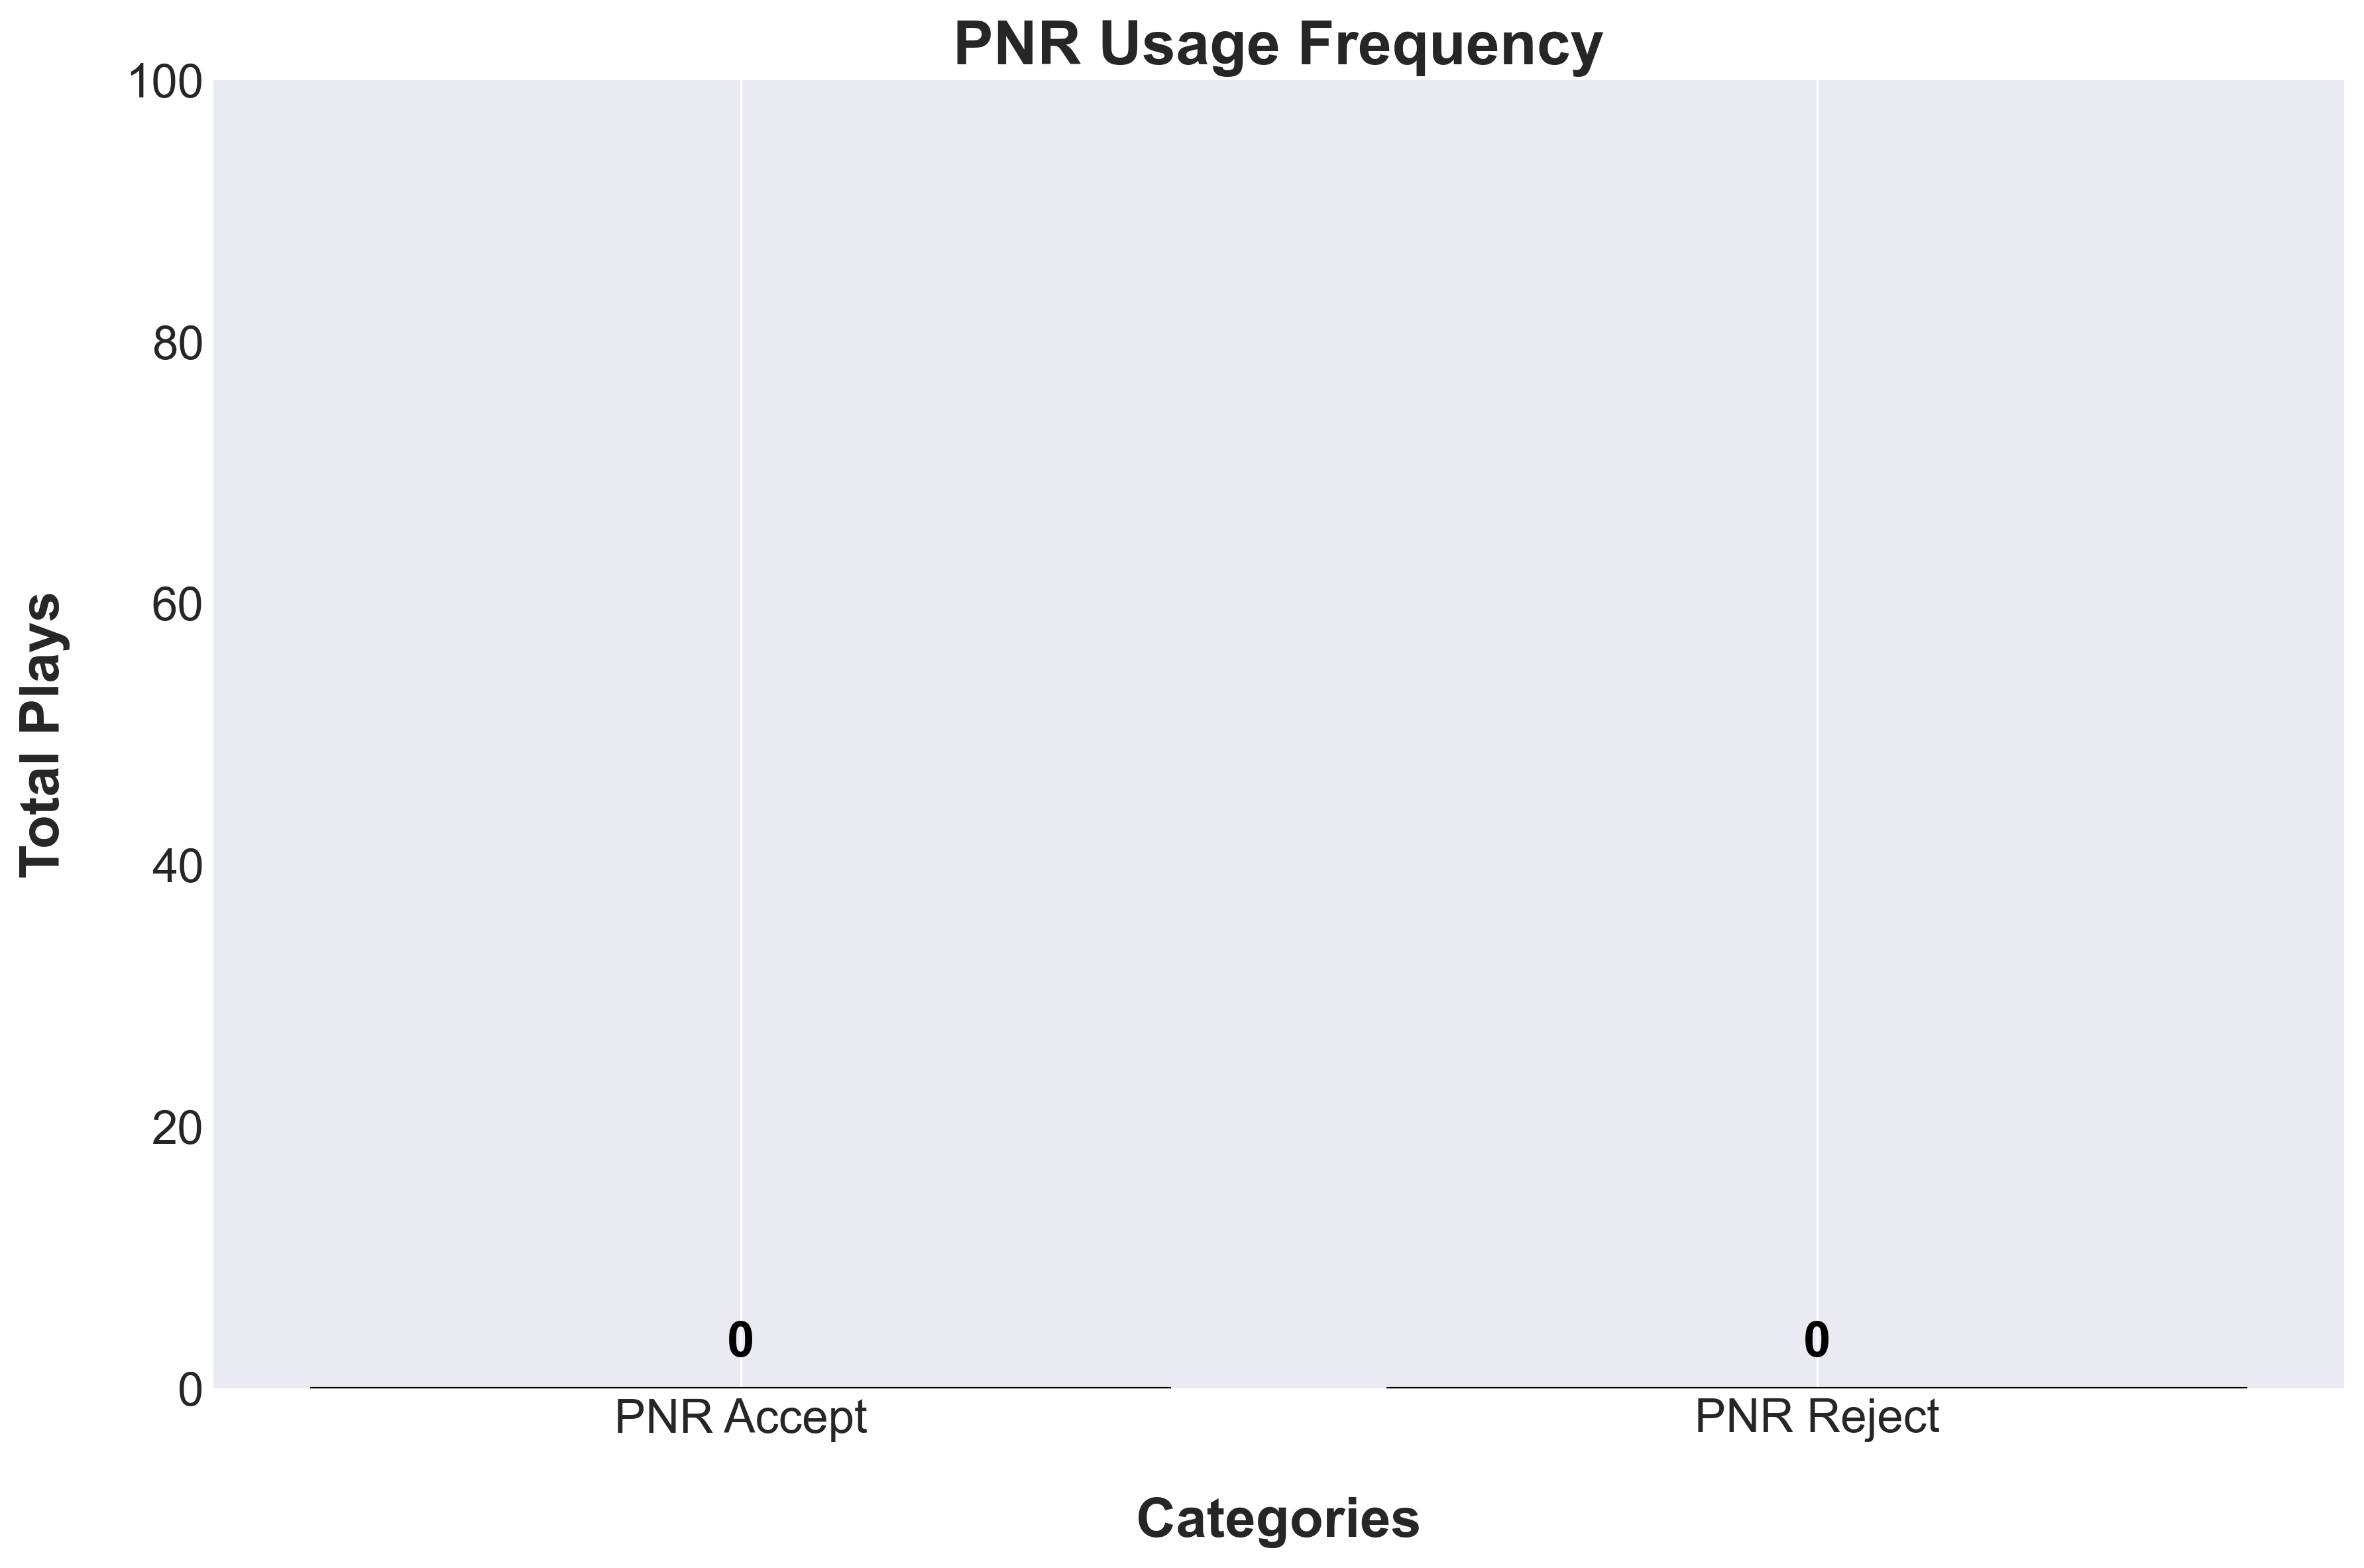
\includegraphics[width=\textwidth, height=.14\textheight]{images/PNR_Usage_Freq.png} % Adjust the width of the image to fit
    \end{minipage}
\end{table}

\vspace{-1em} % Add vertical space before the line (optional)
%\hrule height 1pt width 1\textwidth % Adjust height and width
\vspace{-1em} % Add vertical space after the line (optional)

% PNR Direction / Location Statistics
\begin{table}[H]
    \raisebox{3.5em}{ % Adjust this value to shift the tables vertically
    \begin{minipage}[t]{0.6\textwidth} % Left side (table) takes 85% of the width
        \flushleft
        \centering % Centering the title and the table
        \text{PNR Direction / Location Statistics} % Title above the table in bold
        \vskip .25em % Adds vertical space between title and table
        \scalebox{.6}{ % Scale the entire table down by half
            \renewcommand{\arraystretch}{1.4} % Adjust the number to increase or decrease row spacing
            \begin{tabular}{
            >{\centering\arraybackslash}p{1.75cm} 
            >{\centering\arraybackslash}p{.75cm} 
            >{\centering\arraybackslash}p{.75cm} 
            >{\centering\arraybackslash}p{.75cm} 
            >{\centering\arraybackslash}p{.75cm}
            >{\centering\arraybackslash}p{.75cm} 
            >{\centering\arraybackslash}p{.75cm} 
            >{\centering\arraybackslash}p{.75cm} 
            >{\centering\arraybackslash}p{.75cm}
            >{\centering\arraybackslash}p{.75cm} 
            >{\centering\arraybackslash}p{.75cm}
            >{\centering\arraybackslash}p{.75cm} 
            >{\centering\arraybackslash}p{.75cm}}% Adjust column widths
            \toprule
            {\scriptsize \textbf{PlayType}} &
            {\scriptsize \textbf{Plays}} &
            {\scriptsize \textbf{3PA}} &
            {\scriptsize \textbf{3PM}} &
            {\scriptsize \textbf{3P\%}} & 
            {\scriptsize \textbf{2PA}} & 
            {\scriptsize \textbf{2PM}} & 
            {\scriptsize \textbf{2P\%}} & 
            {\scriptsize \textbf{MiA}} & 
            {\scriptsize \textbf{MiM}} &
            {\scriptsize \textbf{Mi\%}} &
            {\scriptsize \textbf{TO}} &
            {\scriptsize \textbf{Foul}} \\
            \midrule
            
                
            
                
            
                
            
                
            
                
            
                
            
                
            
                
            
                
            
                
            
                
            
                
            
                
            
                
            
                
            
                
            
                
            
                
            
                
            
                
            
                
            
                
            
                
            
                
            
                
            
                
            
                
            
                
            
                
            
                
                    High & 41 & 7 & 3 &
                    42.86 & 
                    23 & 11 &
                    47.83 &
                    7 & 3 &
                    42.86 &
                    7 & 4 \\
                
            
                
                    Left & 16 & 2 & 2 &
                    100.0 & 
                    11 & 4 &
                    36.36 &
                    2 & 0 &
                    0.0 &
                    2 & 1 \\
                
            
                
                    Right & 20 & 3 & 1 &
                    33.33 & 
                    10 & 2 &
                    20.0 &
                    2 & 0 &
                    0.0 &
                    5 & 2 \\
                
            
                
            
                
            
                
            
                
            
                
            
                
            
            \bottomrule
        \end{tabular}
        } % End of \scalebox
    \end{minipage}
    } % End of raisebox, closing the adjustment
    \hfill
    \begin{minipage}[c]{0.35\textwidth} % Right side (image) takes 10% of the width
        \flushright
        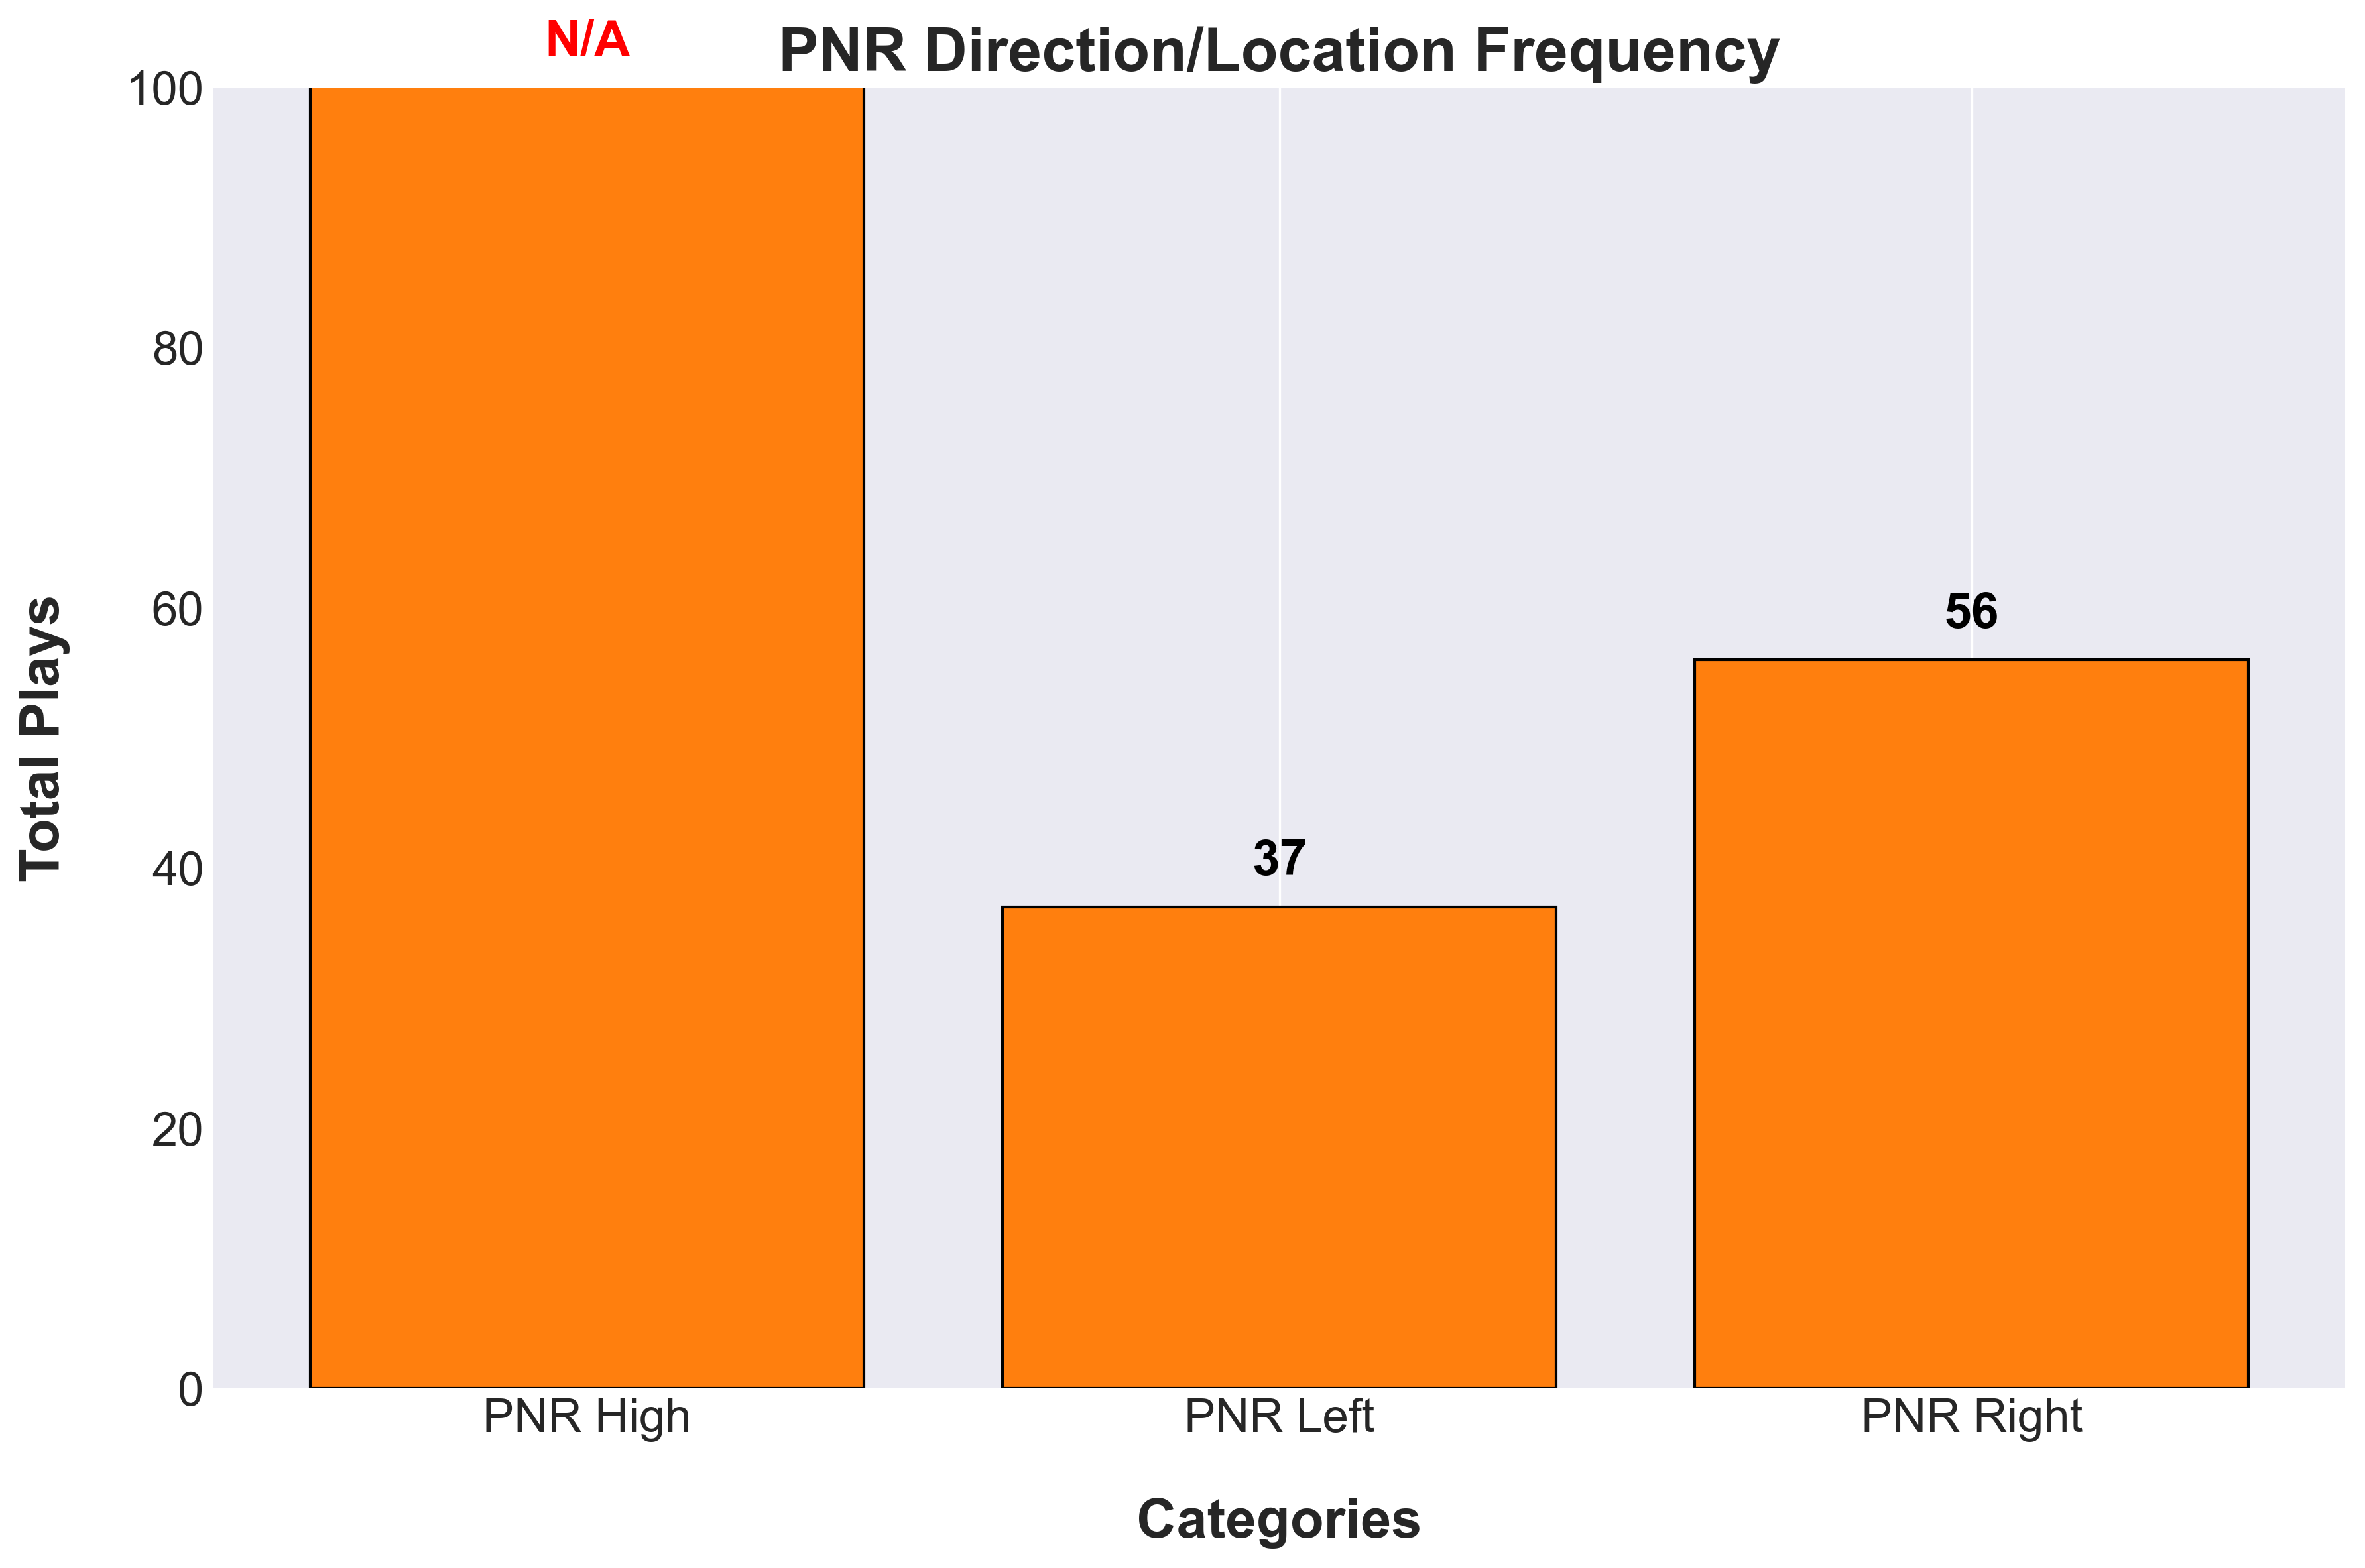
\includegraphics[width=\textwidth, height=.14\textheight]{images/PNR_DirectionLocation_Freq.png} % Adjust the width of the image to fit
    \end{minipage}
    
\end{table}

\vspace{-1em} % Add vertical space before the line (optional)
%\hrule height 1pt width 1\textwidth % Adjust height and width
\vspace{-1em} % Add vertical space after the line (optional)

% PNR Stats for Combination of Usage and Direction Stats
\begin{table}[H]
    \raisebox{4.5em}{ % Adjust this value to shift the tables vertically
    \begin{minipage}[t]{0.6\textwidth} % Left side (table) takes 85% of the width
        \flushleft
        \centering % Centering the title and the table
        \text{PNR Combination Statistics} % Title above the table in bold
        \vskip .25em % Adds vertical space between title and table
        \scalebox{.52}{ % Scale the entire table down by half
            \renewcommand{\arraystretch}{1.4} % Adjust the number to increase or decrease row spacing
            \begin{tabular}{
            >{\centering\arraybackslash}p{4cm} 
            >{\centering\arraybackslash}p{.75cm} 
            >{\centering\arraybackslash}p{.75cm} 
            >{\centering\arraybackslash}p{.75cm} 
            >{\centering\arraybackslash}p{.75cm}
            >{\centering\arraybackslash}p{.75cm} 
            >{\centering\arraybackslash}p{.75cm} 
            >{\centering\arraybackslash}p{.75cm} 
            >{\centering\arraybackslash}p{.75cm}
            >{\centering\arraybackslash}p{.75cm} 
            >{\centering\arraybackslash}p{.75cm}
            >{\centering\arraybackslash}p{.75cm} 
            >{\centering\arraybackslash}p{.75cm}}% Adjust column widths
            \toprule
            {\scriptsize \textbf{PlayType}} &
            {\scriptsize \textbf{Plays}} &
            {\scriptsize \textbf{3PA}} &
            {\scriptsize \textbf{3PM}} &
            {\scriptsize \textbf{3P\%}} & 
            {\scriptsize \textbf{2PA}} & 
            {\scriptsize \textbf{2PM}} & 
            {\scriptsize \textbf{2P\%}} & 
            {\scriptsize \textbf{MiA}} & 
            {\scriptsize \textbf{MiM}} &
            {\scriptsize \textbf{Mi\%}} &
            {\scriptsize \textbf{TO}} &
            {\scriptsize \textbf{Foul}} \\
            \midrule
            
                

            
                

            
                

            
                

            
                

            
                

            
                

            
                

            
                

            
                

            
                

            
                

            
                

            
                

            
                

            
                

            
                

            
                

            
                

            
                

            
                

            
                

            
                

            
                

            
                

            
                

            
                

            
                

            
                

            
                

            
                

            
                

            
                
                    High - Reject & 9 & 1 & 0 &
                    0.0 & 
                    6 & 2 &
                    33.33 &
                    0 & 0 &
                    - &
                    0 & 2 \\
                

            
                
                High - Off & 30 & 4 & 3 &
                    75.0 & 
                    17 & 9 &
                    52.94 &
                    7 & 3 &
                    42.86 &
                    7 & 2 \\
                

            
                
                    Left - Reject & 2 & 0 & 0 &
                    - & 
                    1 & 0 &
                    0.0 &
                    0 & 0 &
                    - &
                    0 & 1 \\
                

            
                
                    Left - Off & 11 & 0 & 0 &
                    - & 
                    9 & 3 &
                    33.33 &
                    2 & 0 &
                    0.0 &
                    2 & 0 \\
                

            
                
                    Right - Reject & 2 & 0 & 0 &
                    - & 
                    1 & 1 &
                    100.0 &
                    0 & 0 &
                    - &
                    1 & 0 \\
                

            
                
                    Right - Off & 15 & 2 & 0 &
                    0.0 & 
                    8 & 1 &
                    12.5 &
                    2 & 0 &
                    0.0 &
                    4 & 1 \\
                

            

            \bottomrule
        \end{tabular}
        } % End of \scalebox
    \end{minipage}
    } % End of raisebox, closing the adjustment
    \hfill % This adds some flexible space between the table and the image
    \begin{minipage}[c]{0.35\textwidth} % Right side (image) takes 10% of the width
        \flushright
        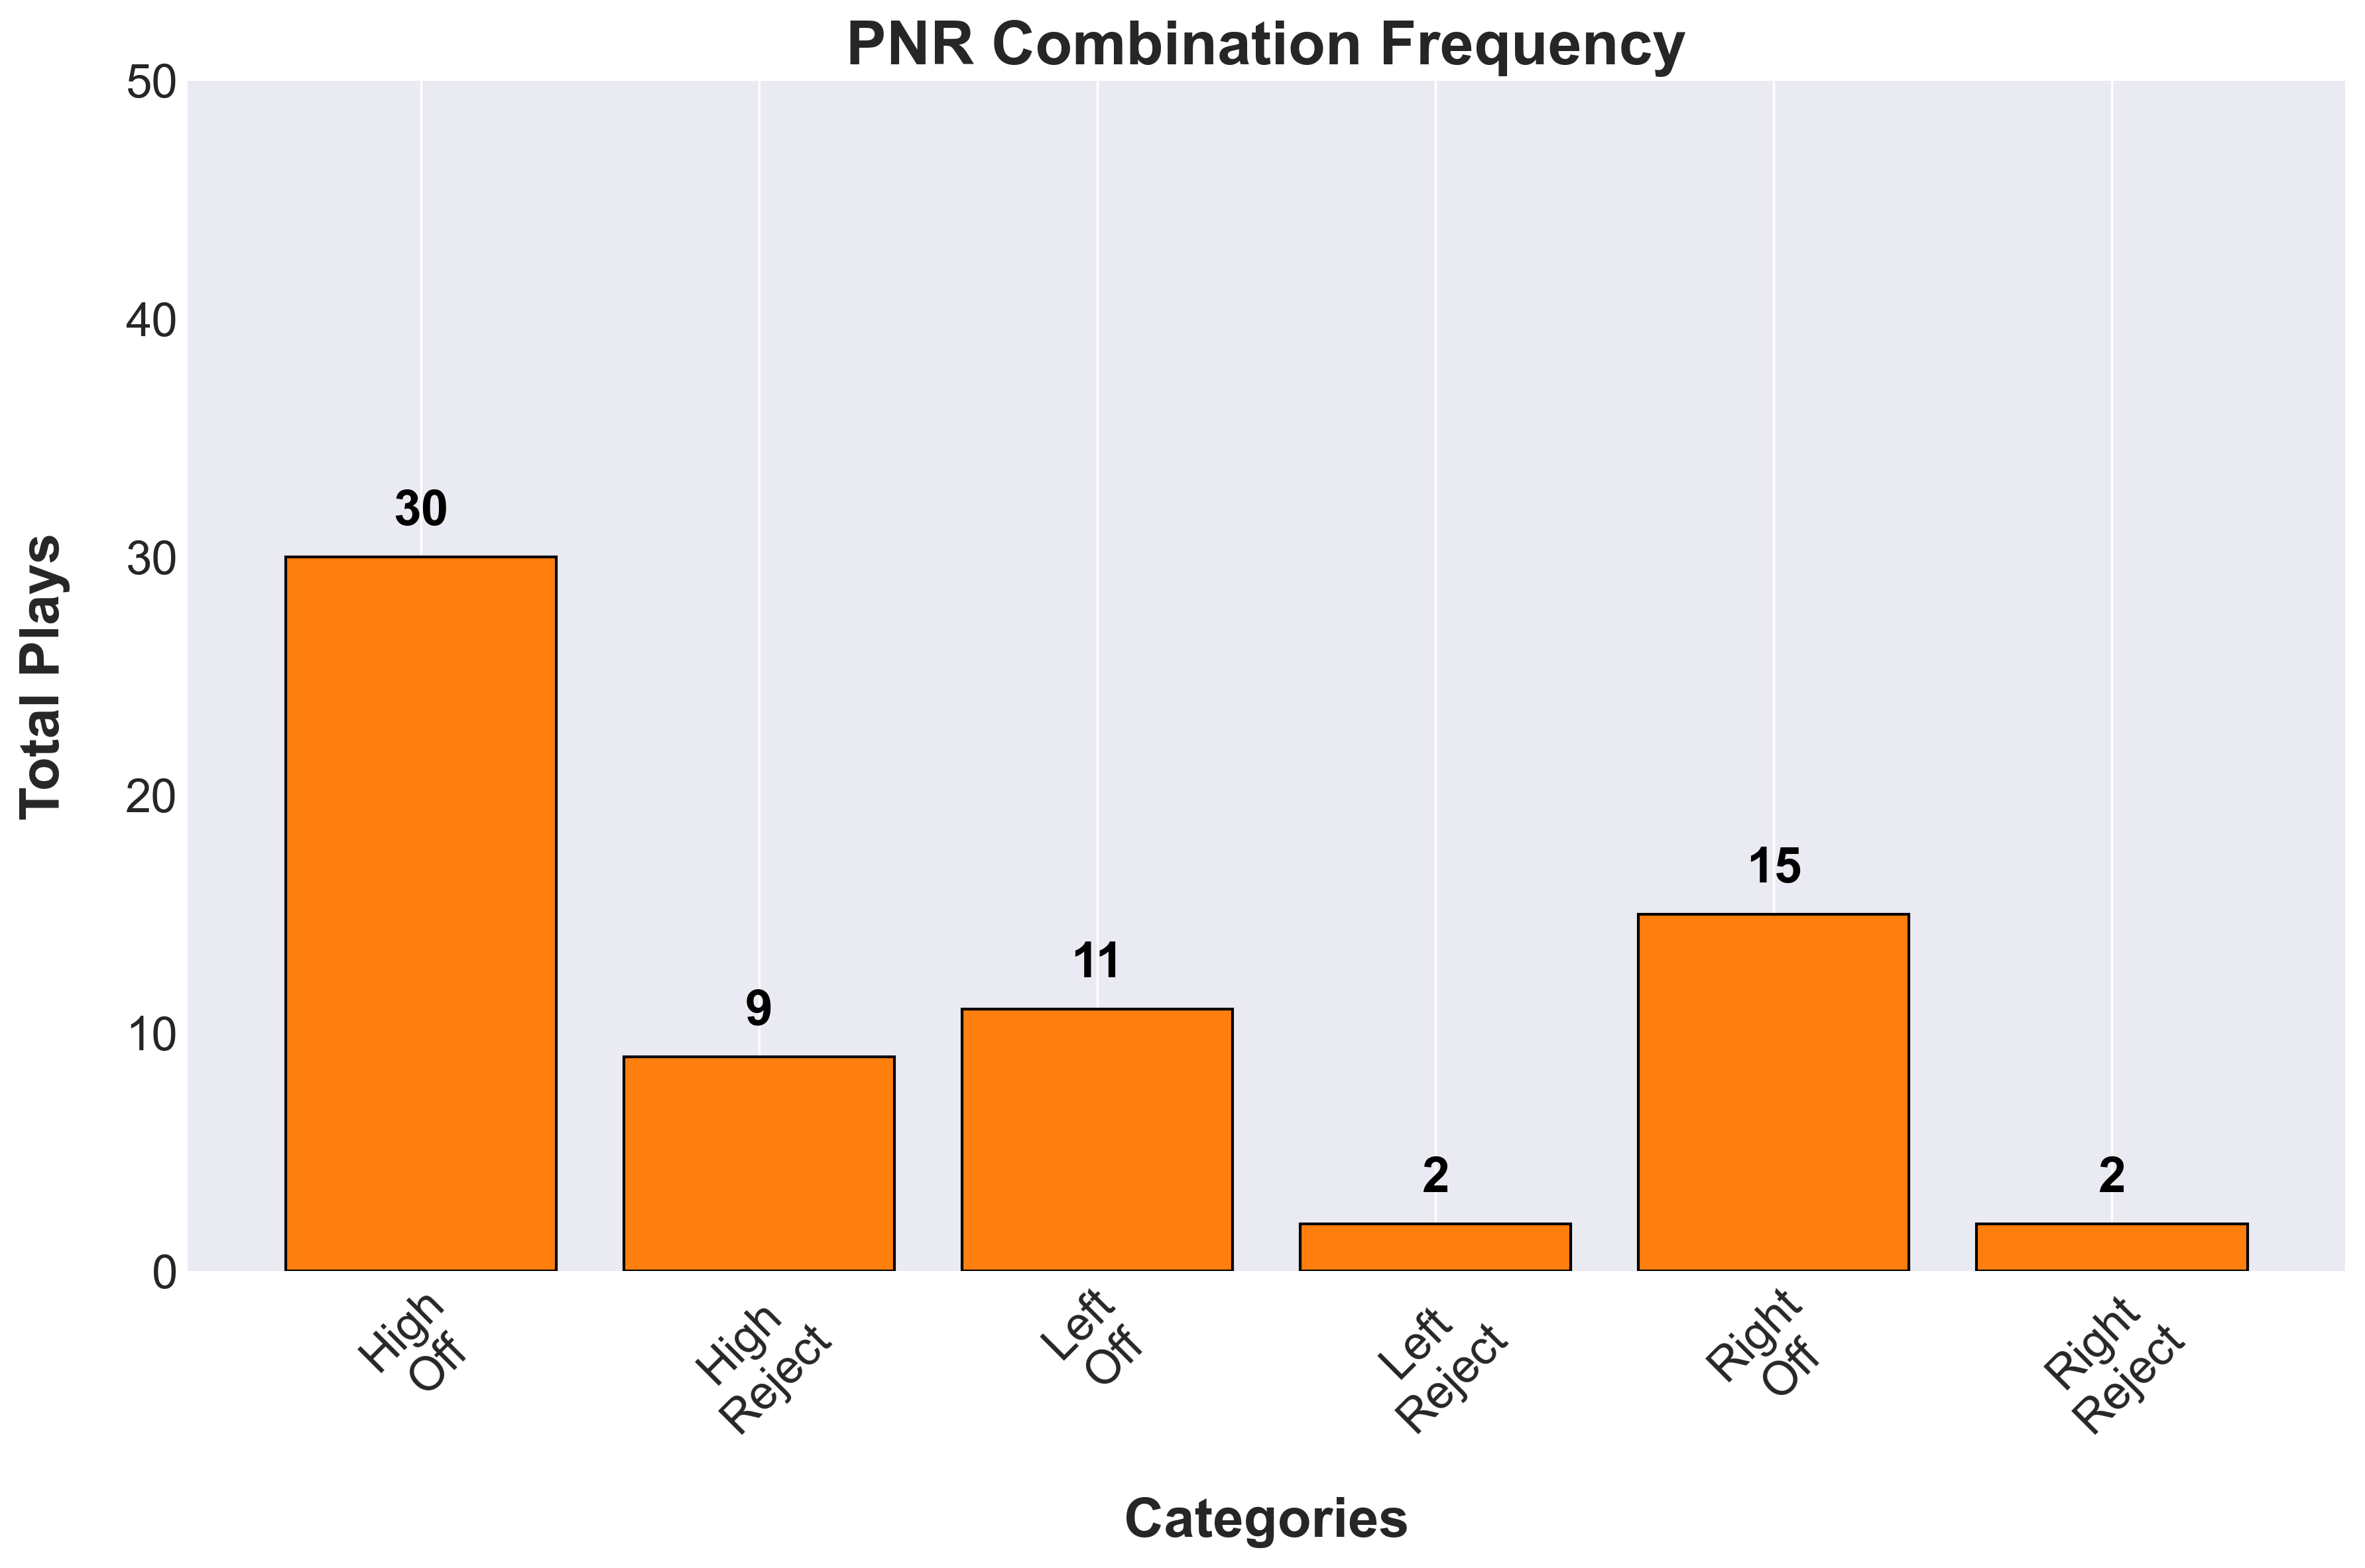
\includegraphics[width=\textwidth, height=.14\textheight]{images/PNR_Combination_Freq.png} % Adjust the width of the image to fit
    \end{minipage}
\end{table}

\vspace{-1em} % Add vertical space before the line (optional)
\hrule height 1pt width 1\textwidth % Adjust height and width
\vspace{1em} % Add vertical space after the line (optional)

\subsubsection{PNR Common Passer Statistics}

% All PNR Passer Statistics Table w/ room for insights
\begin{table}[H]
    \centering
    \begin{minipage}[t]{0.6\textwidth} % Left side (table) takes 85% of the width
        %\flushright
        \centering % Centering the title and the table
        \text{Total Pick N Roll Passer Statistics} % Title above the table in bold
        \vskip .25em % Adds vertical space between title and table
        \scalebox{.85}{ % Scale the entire table down by half
            \scriptsize % Reduce the font size
            \begin{tabular}{
            >{\centering\arraybackslash}p{.75cm} 
            >{\centering\arraybackslash}p{.5cm} 
            >{\centering\arraybackslash}p{.5cm} 
            >{\centering\arraybackslash}p{.5cm}
            >{\centering\arraybackslash}p{.5cm} 
            >{\centering\arraybackslash}p{.5cm} 
            >{\centering\arraybackslash}p{.5cm} 
            >{\centering\arraybackslash}p{.5cm}
            >{\centering\arraybackslash}p{.5cm} 
            >{\centering\arraybackslash}p{.5cm}
            >{\centering\arraybackslash}p{.5cm} 
            >{\centering\arraybackslash}p{.5cm}}% Adjust column widths
            \toprule
            \textbf{Plays} &
            \textbf{3PA} &
            \textbf{3PM} &
            \textbf{3P\%} & 
            \textbf{2PA} & 
            \textbf{2PM} & 
            \textbf{2P\%} & 
            \textbf{MiA} & 
            \textbf{MiM} &
            \textbf{Mi\%} &
            \textbf{TO} &
            \textbf{Foul} \\
            \midrule
            
                
            
                
                    70 & 37 & 9 &
                    20.24 & 
                    24 & 13 &
                    62.26 &
                    3 & 1 &
                    50.0 &
                    4 & 5 \\
                
            
                
            
                
            
                
            
                
            
                
            
                
            
                
            
                
            
                
            
                
            
                
            
                
            
                
            
                
            
                
            
                
            
                
            
                
            
                
            
                
            
                
            
                
            
                
            
                
            
                
            
                
            
                
            
                
            
                
            
                
            
                
            
                
            
                
            
                
            
                
            
                
            
            \bottomrule
            \end{tabular}
        }
    \end{minipage}
\end{table}

\vspace{-1em} % Add vertical space before the line (optional)
%\hrule height 1pt width 1\textwidth % Adjust height and width
\vspace{0em} % Add vertical space after the line (optional)

% PNR -> Different PlayType Statistics
\begin{table}[H]
    \raisebox{3em}{ % Adjust this value to shift the tables vertically
    \begin{minipage}[t]{0.6\textwidth} % Left side (table) takes 85% of the width
        \flushleft
        \centering % Centering the title and the table
        \text{PNR to Different PlayType Statistics} % Title above the table in bold
        \vskip .25em % Adds vertical space between title and table
        \scalebox{.6}{ % Scale the entire table
            \scriptsize % Reduce the font size
            \renewcommand{\arraystretch}{1.3} % Adjust the number to increase or decrease row spacing
            \begin{tabular}{
            >{\centering\arraybackslash}p{1.5cm} 
            >{\centering\arraybackslash}p{.75cm} 
            >{\centering\arraybackslash}p{.75cm} 
            >{\centering\arraybackslash}p{.75cm} 
            >{\centering\arraybackslash}p{.75cm}
            >{\centering\arraybackslash}p{.75cm} 
            >{\centering\arraybackslash}p{.75cm} 
            >{\centering\arraybackslash}p{.75cm} 
            >{\centering\arraybackslash}p{.75cm}
            >{\centering\arraybackslash}p{.75cm} 
            >{\centering\arraybackslash}p{.75cm}
            >{\centering\arraybackslash}p{.75cm} 
            >{\centering\arraybackslash}p{.75cm}}% Adjust column widths
            \toprule
            {\scriptsize \textbf{PlayType}} &
            {\scriptsize \textbf{Plays}} &
            {\scriptsize \textbf{3PA}} &
            {\scriptsize \textbf{3PM}} &
            {\scriptsize \textbf{3P\%}} & 
            {\scriptsize \textbf{2PA}} & 
            {\scriptsize \textbf{2PM}} & 
            {\scriptsize \textbf{2P\%}} & 
            {\scriptsize \textbf{MiA}} & 
            {\scriptsize \textbf{MiM}} &
            {\scriptsize \textbf{Mi\%}} &
            {\scriptsize \textbf{TO}} &
            {\scriptsize \textbf{Foul}} \\
            \midrule
            
                
            
                
            
                
                    Cuts & 5 & 0 & 0 &
                    - & 
                    4 & 4 &
                    100.0 &
                    0 & 0 &
                    - &
                    0 & 1 \\
                
            
                
                    S.U Drives & 15 & 3 & 0 &
                    0.0 & 
                    6 & 3 &
                    50.0 &
                    0 & 0 &
                    - &
                    4 & 2 \\
                
            
                
                    S.U Shots & 30 & 28 & 8 &
                    27.78 & 
                    2 & 0 &
                    0.0 &
                    2 & 0 &
                    0.0 &
                    0 & 0 \\
                
            
                
                    Rollman & 20 & 6 & 1 &
                    16.67 & 
                    12 & 6 &
                    48.57 &
                    1 & 1 &
                    100.0 &
                    0 & 2 \\
                
            
                
            
                
            
                
            
                
            
                
            
                
            
                
            
                
            
                
            
                
            
                
            
                
            
                
            
                
            
                
            
                
            
                
            
                
            
                
            
                
            
                
            
                
            
                
            
                
            
                
            
                
            
                
            
                
            
                
            
                
            
                
            
                
            

            \bottomrule
        \end{tabular}
        }
    \end{minipage}
    }
    \hfill % This adds some flexible space between the table and the image
    \begin{minipage}[c]{0.35\textwidth} % Right side (image) takes 10% of the width
        \flushright
        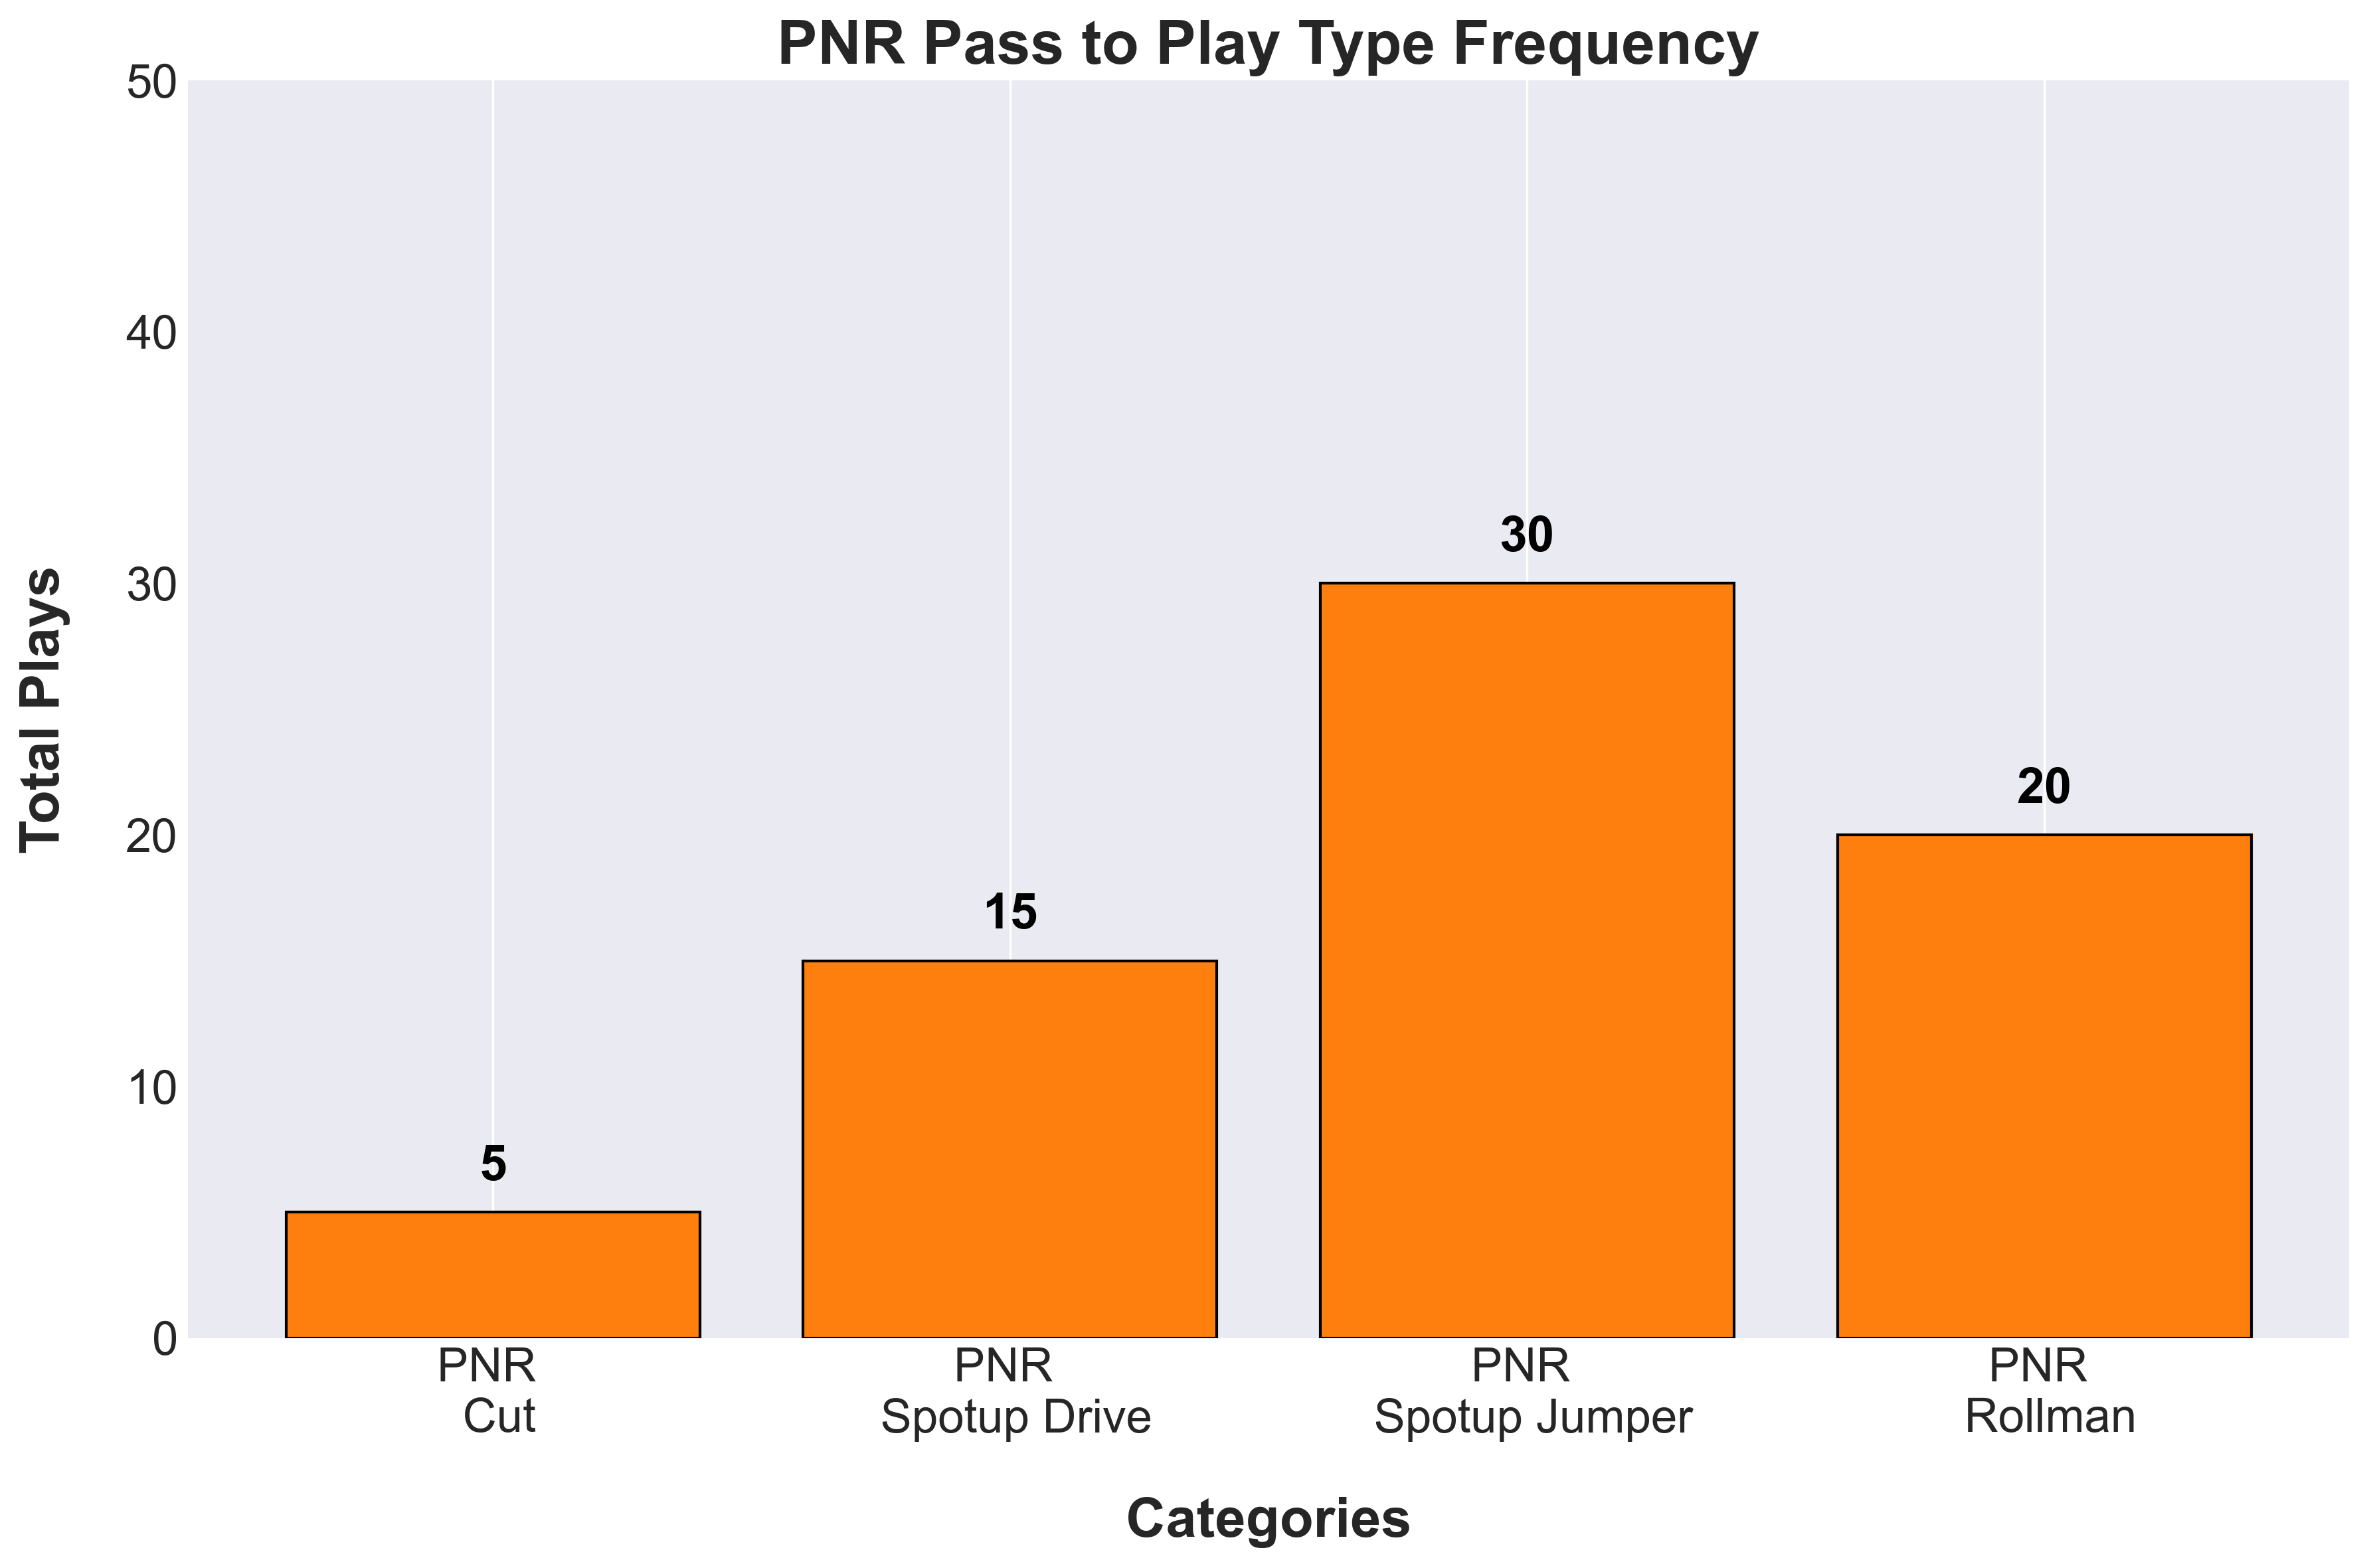
\includegraphics[width=\textwidth, height=.14\textheight]{images/PNR_PassPlayType_Freq.png} % Adjust the width of the image to fit
    \end{minipage}
\end{table}

\vspace{-1em} % Add vertical space before the line (optional)
\hrule height 1pt width 1\textwidth % Adjust height and width
\vspace{1em} % Add vertical space after the line (optional)

\subsubsection{BH High PNR Passer Statistics}

% BH High -> Cuts Secondary Player Stats
\begin{table}[H]
    \raisebox{3em}{ % Adjust this value to shift the tables vertically
    \begin{minipage}[t]{0.6\textwidth} % Left side (table) takes 85% of the width
        \flushleft
        \centering % Centering the title and the table
        \text{BH High - Cuts Player Statistics} % Title above the table in bold
        \vskip .25em % Adds vertical space between title and table
        \scalebox{.6}{ % Scale the entire table down by half
            \renewcommand{\arraystretch}{1.4} % Adjust the number to increase or decrease row spacing
            \begin{tabular}{
            >{\centering\arraybackslash}p{3cm} 
            >{\centering\arraybackslash}p{.75cm} 
            >{\centering\arraybackslash}p{.75cm} 
            >{\centering\arraybackslash}p{.75cm} 
            >{\centering\arraybackslash}p{.75cm}
            >{\centering\arraybackslash}p{.75cm} 
            >{\centering\arraybackslash}p{.75cm}
            >{\centering\arraybackslash}p{.75cm}
            >{\centering\arraybackslash}p{.75cm} 
            >{\centering\arraybackslash}p{.75cm}}% Adjust column widths
            \toprule
            {\scriptsize \textbf{Player}} &
            {\scriptsize \textbf{Plays}} &
            {\scriptsize \textbf{2PA}} & 
            {\scriptsize \textbf{2PM}} & 
            {\scriptsize \textbf{2P\%}} & 
            {\scriptsize \textbf{MiA}} & 
            {\scriptsize \textbf{MiM}} &
            {\scriptsize \textbf{Mi\%}} &
            {\scriptsize \textbf{TO}} &
            {\scriptsize \textbf{Foul}} \\
            \midrule
            
                
            
                
            
                
            
                
            
                
            
                
            
                
                    
                        Keegan Ocorr & 
                        2 & 
                        1 & 
                        1 & 
                        100.0 & 
                        0 & 
                        0 & 
                        - & 
                        0 & 
                        1 \\
                    
                        Luke Granto & 
                        1 & 
                        1 & 
                        1 & 
                        100.0 & 
                        0 & 
                        0 & 
                        - & 
                        0 & 
                        0 \\
                    
                        Zac Ditzel & 
                        1 & 
                        1 & 
                        1 & 
                        100.0 & 
                        0 & 
                        0 & 
                        - & 
                        0 & 
                        0 \\
                    
                
            
                
            
                
            
                
            
                
            
                
            
                
            
                
            
                
            
                
            
                
            
                
            
                
            
                
            
                
            
                
            
                
            
                
            
                
            
                
            
                
            
                
            
                
            
                
            
                
            
                
            
                
            
                
            
                
            
                
            
                
            
                
            
            \bottomrule
        \end{tabular}
        } % End of \scalebox
    \end{minipage}
    } % End of raisebox, closing the adjustment
    \hfill % This adds some flexible space between the table and the image
    \begin{minipage}[c]{0.35\textwidth} % Right side (image) takes 10% of the width
        \flushright
        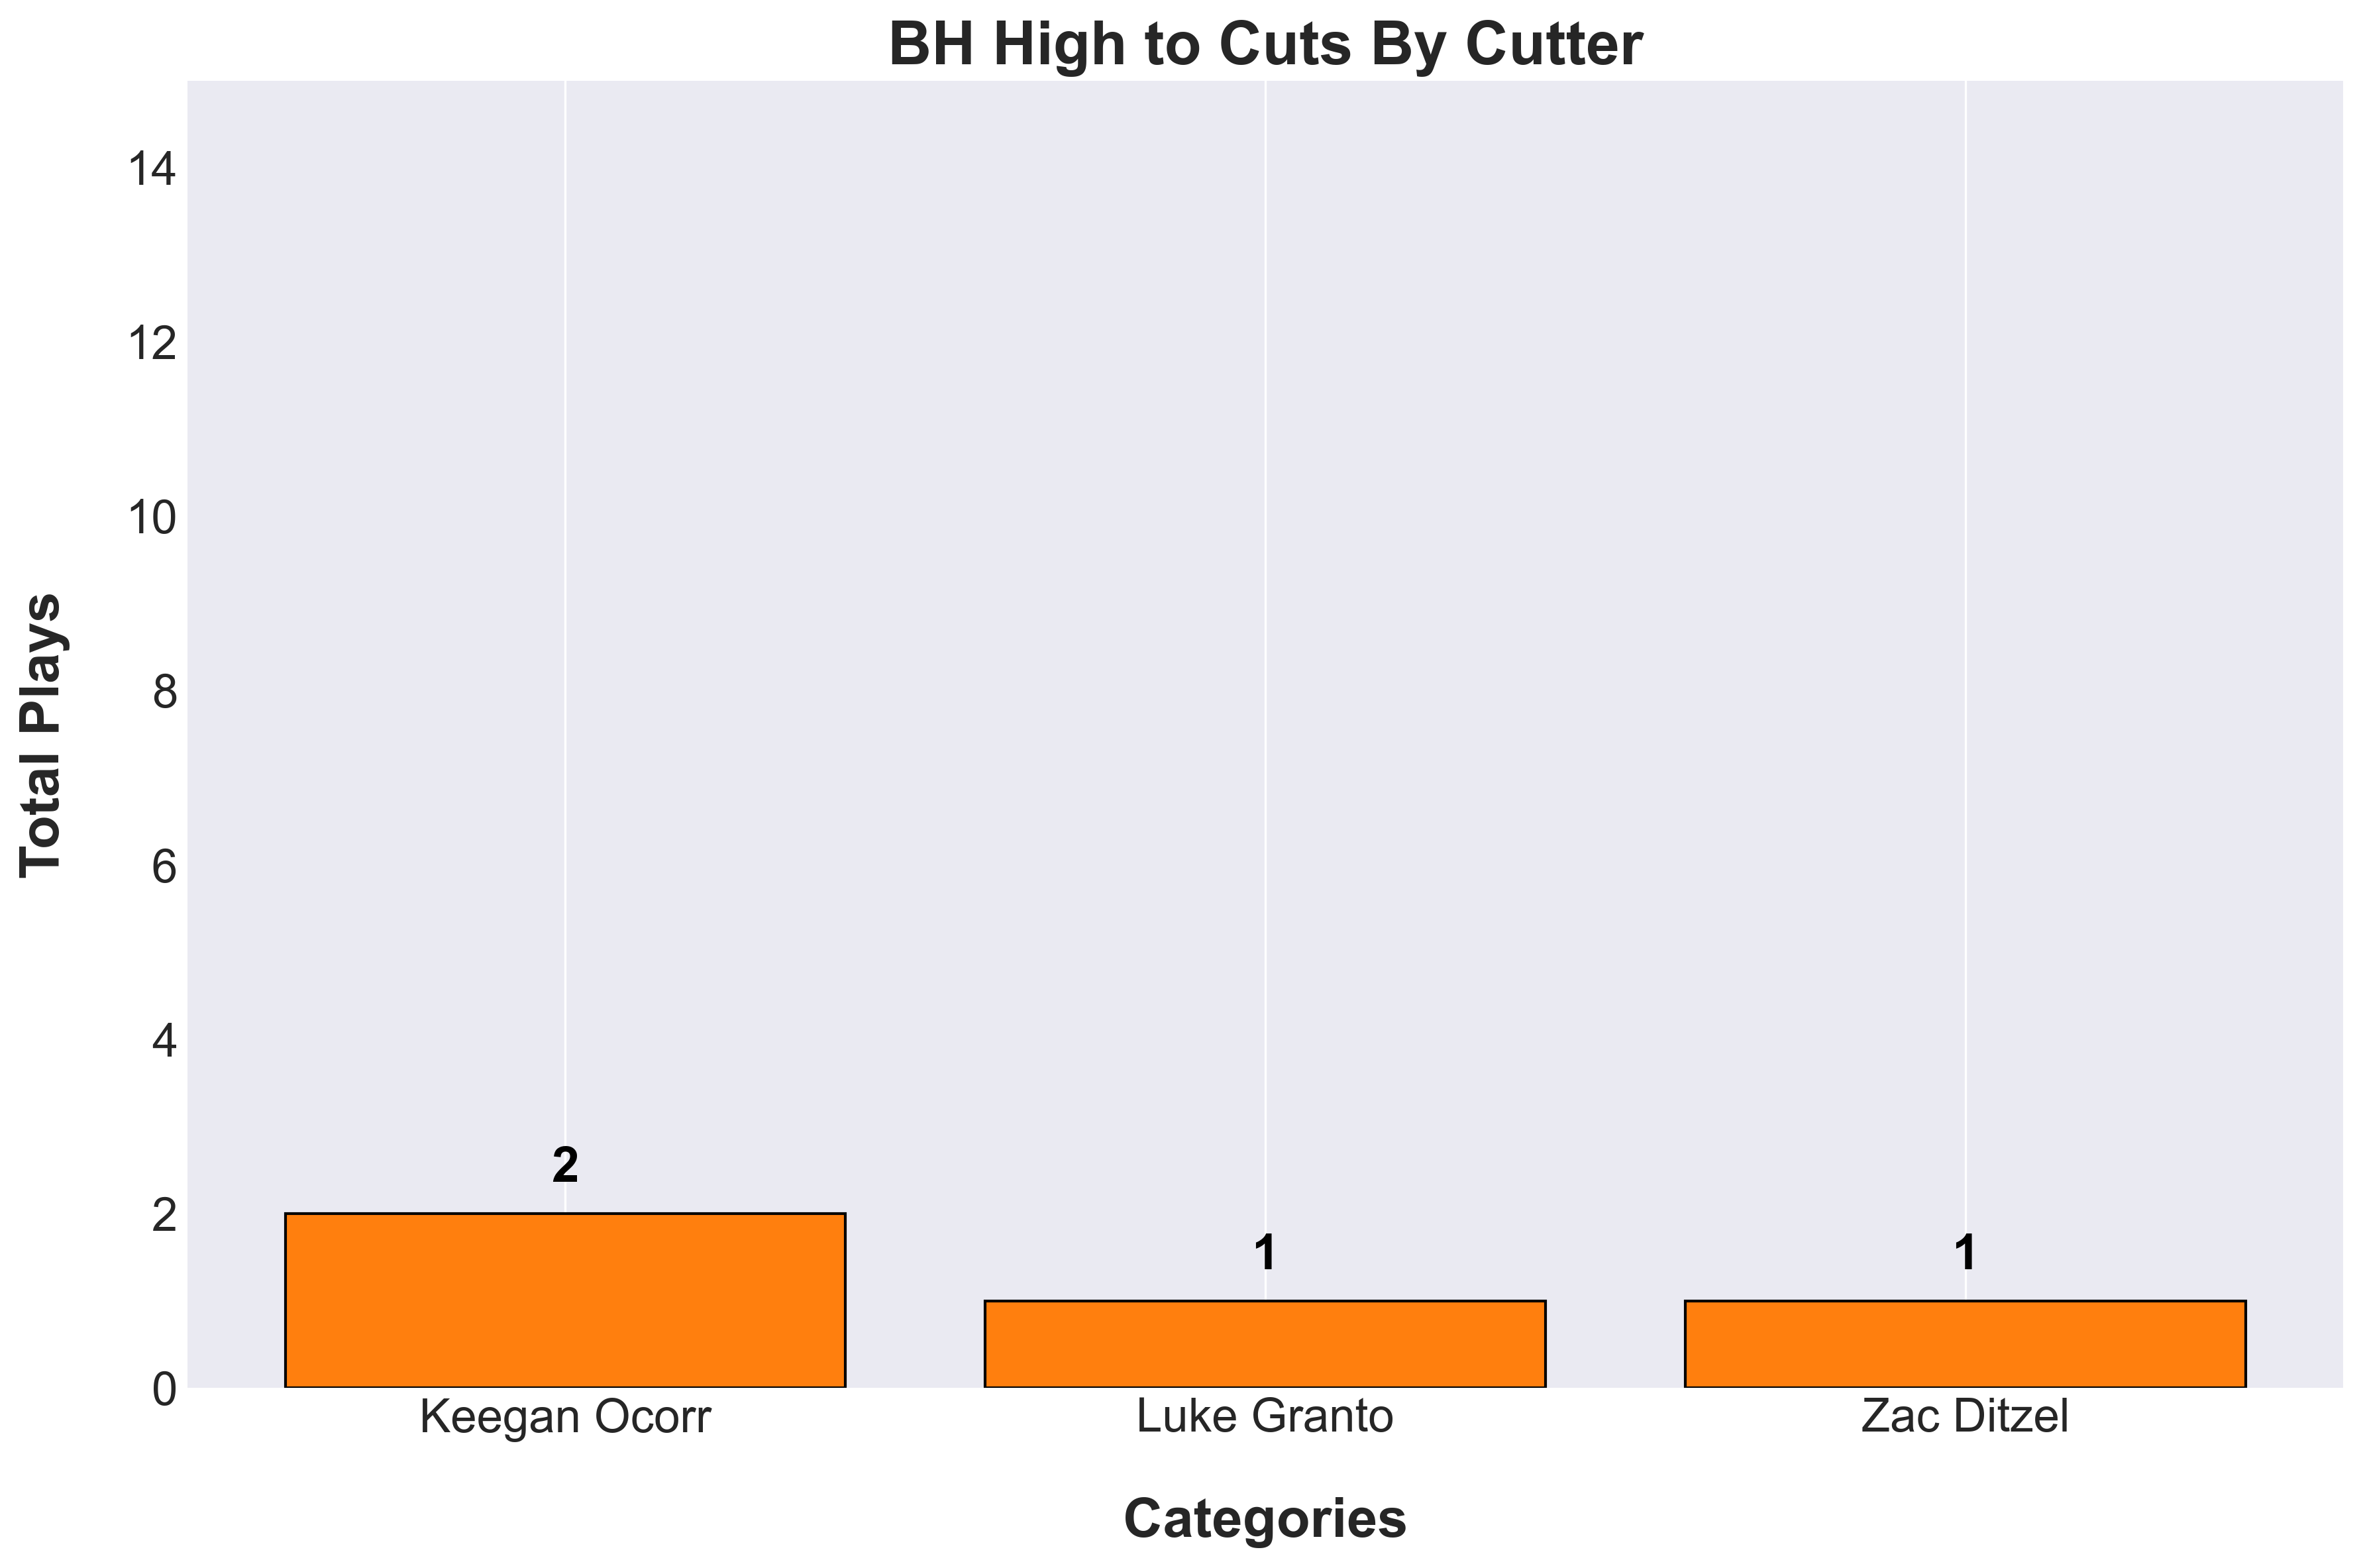
\includegraphics[width=\textwidth, height=.14\textheight]{images/PNR_PassHighCutsPlayer_Freq.png} % Adjust the width of the image to fit
    \end{minipage}
\end{table}

\vspace{-1em} % Add vertical space before the line (optional)
%\hrule height 1pt width 1\textwidth % Adjust height and width
\vspace{-1em} % Add vertical space after the line (optional)

% BH High -> Spot Up Drives Secondary Player Stats
\begin{table}[H]
    \raisebox{3em}{ % Adjust this value to shift the tables vertically
    \begin{minipage}[t]{0.6\textwidth} % Left side (table) takes 85% of the width
        \flushleft
        \centering % Centering the title and the table
        \text{BH High - Spot Up Drives Player Statistics} % Title above the table in bold
        \vskip .25em % Adds vertical space between title and table
        \scalebox{.55}{ % Scale the entire table down by half
            \renewcommand{\arraystretch}{1.4} % Adjust the number to increase or decrease row spacing
            \begin{tabular}{
            >{\centering\arraybackslash}p{3cm} 
            >{\centering\arraybackslash}p{.75cm} 
            >{\centering\arraybackslash}p{.75cm} 
            >{\centering\arraybackslash}p{.75cm} 
            >{\centering\arraybackslash}p{.75cm}
            >{\centering\arraybackslash}p{.75cm} 
            >{\centering\arraybackslash}p{.75cm} 
            >{\centering\arraybackslash}p{.75cm} 
            >{\centering\arraybackslash}p{.75cm}
            >{\centering\arraybackslash}p{.75cm} 
            >{\centering\arraybackslash}p{.75cm}
            >{\centering\arraybackslash}p{.75cm} 
            >{\centering\arraybackslash}p{.75cm}}% Adjust column widths
            \toprule
            {\scriptsize \textbf{Player}} &
            {\scriptsize \textbf{Plays}} &
            {\scriptsize \textbf{3PA}} &
            {\scriptsize \textbf{3PM}} &
            {\scriptsize \textbf{3P\%}} & 
            {\scriptsize \textbf{2PA}} & 
            {\scriptsize \textbf{2PM}} & 
            {\scriptsize \textbf{2P\%}} & 
            {\scriptsize \textbf{MiA}} & 
            {\scriptsize \textbf{MiM}} &
            {\scriptsize \textbf{Mi\%}} &
            {\scriptsize \textbf{TO}} &
            {\scriptsize \textbf{Foul}} \\
            \midrule
            
                
            
                
            
                
            
                
            
                
            
                
            
                
            
                
                    
                        Brock Bowen & 
                        2 & 
                        1 & 
                        0 & 
                        0.0 & 
                        1 & 
                        1 & 
                        100.0 & 
                        0 & 
                        0 & 
                        - & 
                        0 & 
                        0 \\
                    
                        Brody Brown & 
                        1 & 
                        0 & 
                        0 & 
                        - & 
                        0 & 
                        0 & 
                        - & 
                        0 & 
                        0 & 
                        - & 
                        1 & 
                        0 \\
                    
                        Keegan Ocorr & 
                        4 & 
                        0 & 
                        0 & 
                        - & 
                        1 & 
                        1 & 
                        100.0 & 
                        0 & 
                        0 & 
                        - & 
                        2 & 
                        1 \\
                    
                        Mark Osime & 
                        1 & 
                        0 & 
                        0 & 
                        - & 
                        1 & 
                        0 & 
                        0.0 & 
                        0 & 
                        0 & 
                        - & 
                        0 & 
                        0 \\
                    
                        Zac Ditzel & 
                        2 & 
                        1 & 
                        0 & 
                        0.0 & 
                        1 & 
                        1 & 
                        100.0 & 
                        0 & 
                        0 & 
                        - & 
                        0 & 
                        0 \\
                    
                
            
                
            
                
            
                
            
                
            
                
            
                
            
                
            
                
            
                
            
                
            
                
            
                
            
                
            
                
            
                
            
                
            
                
            
                
            
                
            
                
            
                
            
                
            
                
            
                
            
                
            
                
            
                
            
                
            
                
            
                
            

            \bottomrule
        \end{tabular}
        } % End of \scalebox
    \end{minipage}
    } % End of raisebox, closing the adjustment
    \hfill % This adds some flexible space between the table and the image
    \begin{minipage}[c]{0.35\textwidth} % Right side (image) takes 10% of the width
        \flushright
        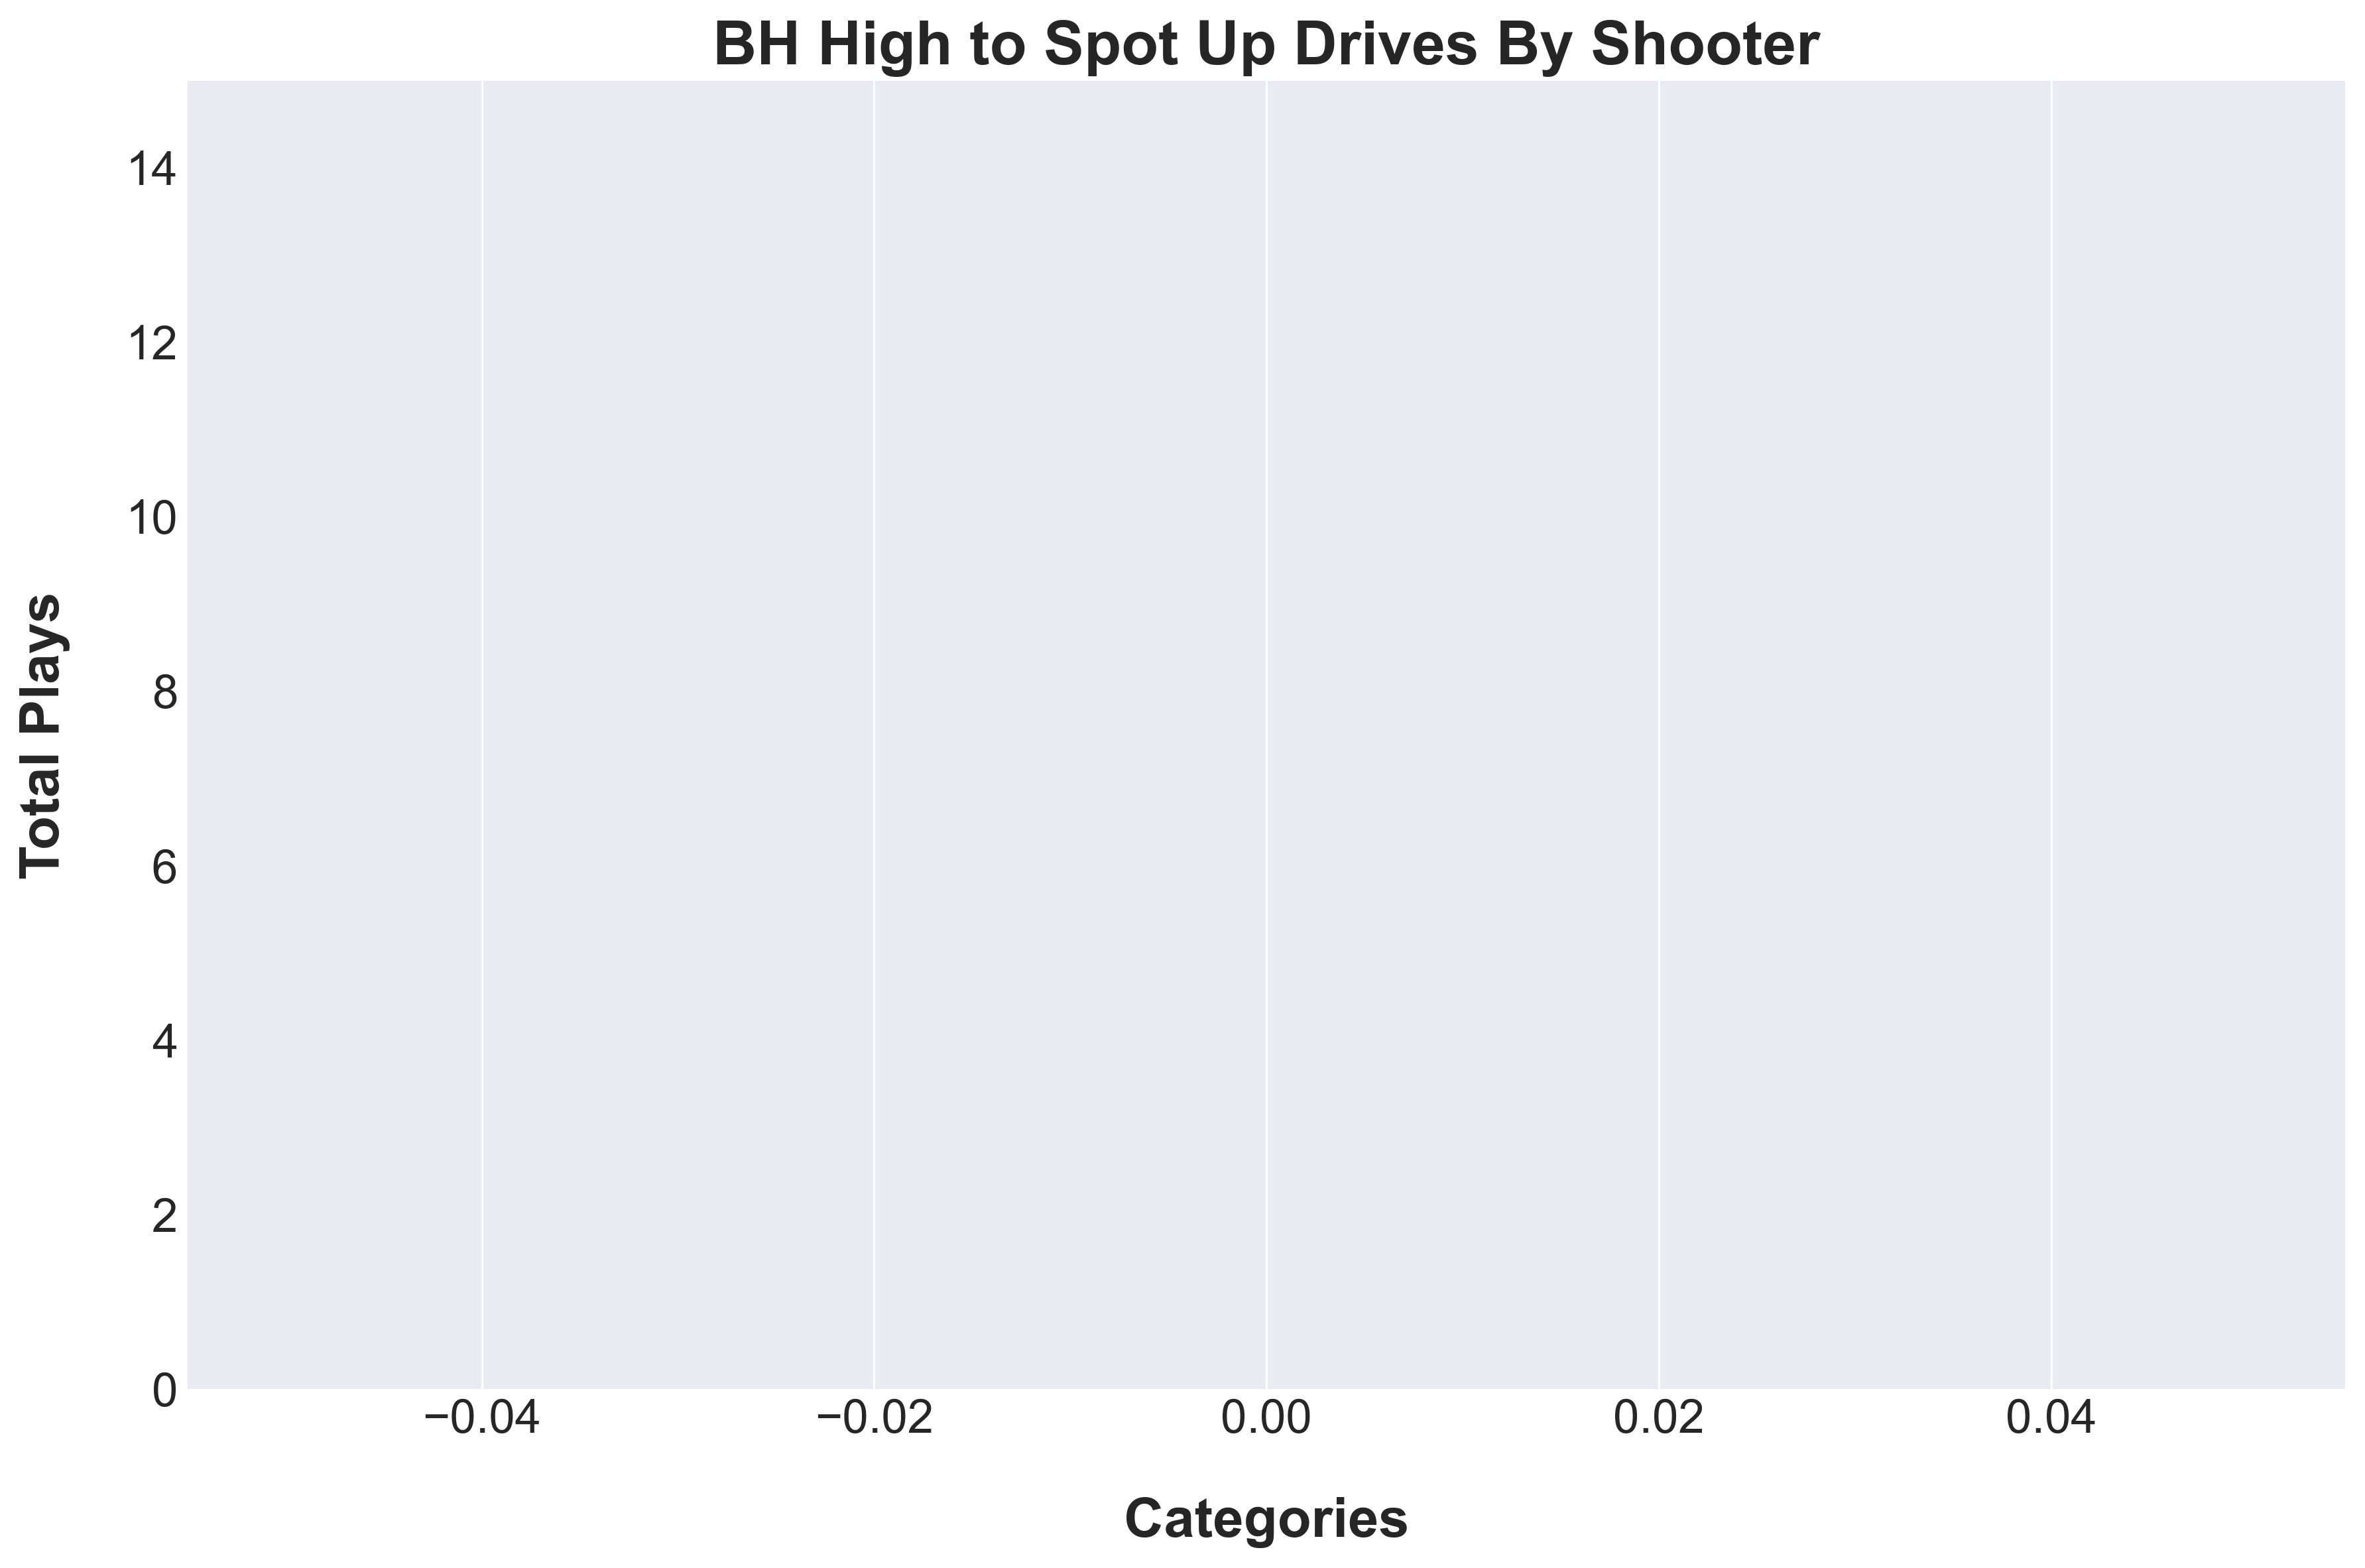
\includegraphics[width=\textwidth, height=.14\textheight]{images/PNR_PassHighDrivesPlayer_Freq.png} % Adjust the width of the image to fit
    \end{minipage}
\end{table}

\vspace{-1em} % Add vertical space before the line (optional)
%\hrule height 1pt width 1\textwidth % Adjust height and width
\vspace{-1em} % Add vertical space after the line (optional)

% BH High -> Spot Up Shots Secondary Player Stats
\begin{table}[H]
    \raisebox{3em}{ % Adjust this value to shift the tables vertically
    \begin{minipage}[t]{0.6\textwidth} % Left side (table) takes 85% of the width
        \flushleft
        \centering % Centering the title and the table
        \text{BH High - Spot Up Shots Player Statistics} % Title above the table in bold
        \vskip .25em % Adds vertical space between title and table
        \scalebox{.6}{ % Scale the entire table down by half
            \renewcommand{\arraystretch}{1.4} % Adjust the number to increase or decrease row spacing
            \begin{tabular}{
            >{\centering\arraybackslash}p{3cm} 
            >{\centering\arraybackslash}p{.75cm} 
            >{\centering\arraybackslash}p{.75cm} 
            >{\centering\arraybackslash}p{.75cm} 
            >{\centering\arraybackslash}p{.75cm} 
            >{\centering\arraybackslash}p{.75cm}
            >{\centering\arraybackslash}p{.75cm} 
            >{\centering\arraybackslash}p{.75cm}
            >{\centering\arraybackslash}p{.75cm} 
            >{\centering\arraybackslash}p{.75cm}}% Adjust column widths
            \toprule
            {\scriptsize \textbf{Player}} &
            {\scriptsize \textbf{Plays}} &
            {\scriptsize \textbf{3PA}} &
            {\scriptsize \textbf{3PM}} &
            {\scriptsize \textbf{3P\%}} & 
            {\scriptsize \textbf{MiA}} & 
            {\scriptsize \textbf{MiM}} &
            {\scriptsize \textbf{Mi\%}} &
            {\scriptsize \textbf{TO}} &
            {\scriptsize \textbf{Foul}} \\
            \midrule
            
                
            
                
            
                
            
                
            
                
            
                
            
                
            
                
            
                
                    
                        Brandon Weiss & 
                        2 & 
                        2 & 
                        1 & 
                        50.0 & 
                        0 & 
                        0 & 
                        - & 
                        0 & 
                        0 \\
                    
                        Brock Bowen & 
                        7 & 
                        7 & 
                        4 & 
                        57.14 & 
                        0 & 
                        0 & 
                        - & 
                        0 & 
                        0 \\
                    
                        Brody Brown & 
                        5 & 
                        5 & 
                        0 & 
                        0.0 & 
                        0 & 
                        0 & 
                        - & 
                        0 & 
                        0 \\
                    
                        Jackson Otis & 
                        2 & 
                        2 & 
                        1 & 
                        50.0 & 
                        0 & 
                        0 & 
                        - & 
                        0 & 
                        0 \\
                    
                        Keegan Ocorr & 
                        1 & 
                        1 & 
                        0 & 
                        0.0 & 
                        0 & 
                        0 & 
                        - & 
                        0 & 
                        0 \\
                    
                        Kenny Wilburn & 
                        2 & 
                        1 & 
                        1 & 
                        100.0 & 
                        1 & 
                        0 & 
                        0.0 & 
                        0 & 
                        0 \\
                    
                        Mark Osime & 
                        1 & 
                        1 & 
                        0 & 
                        0.0 & 
                        0 & 
                        0 & 
                        - & 
                        0 & 
                        0 \\
                    
                        Ronnie Toole & 
                        1 & 
                        1 & 
                        0 & 
                        0.0 & 
                        0 & 
                        0 & 
                        - & 
                        0 & 
                        0 \\
                    
                
            
                
            
                
            
                
            
                
            
                
            
                
            
                
            
                
            
                
            
                
            
                
            
                
            
                
            
                
            
                
            
                
            
                
            
                
            
                
            
                
            
                
            
                
            
                
            
                
            
                
            
                
            
                
            
                
            
                
            

            \bottomrule
        \end{tabular}
        } % End of \scalebox
    \end{minipage}
    } % End of raisebox, closing the adjustment
    \hfill % This adds some flexible space between the table and the image
    \begin{minipage}[c]{0.35\textwidth} % Right side (image) takes 10% of the width
        \flushright
        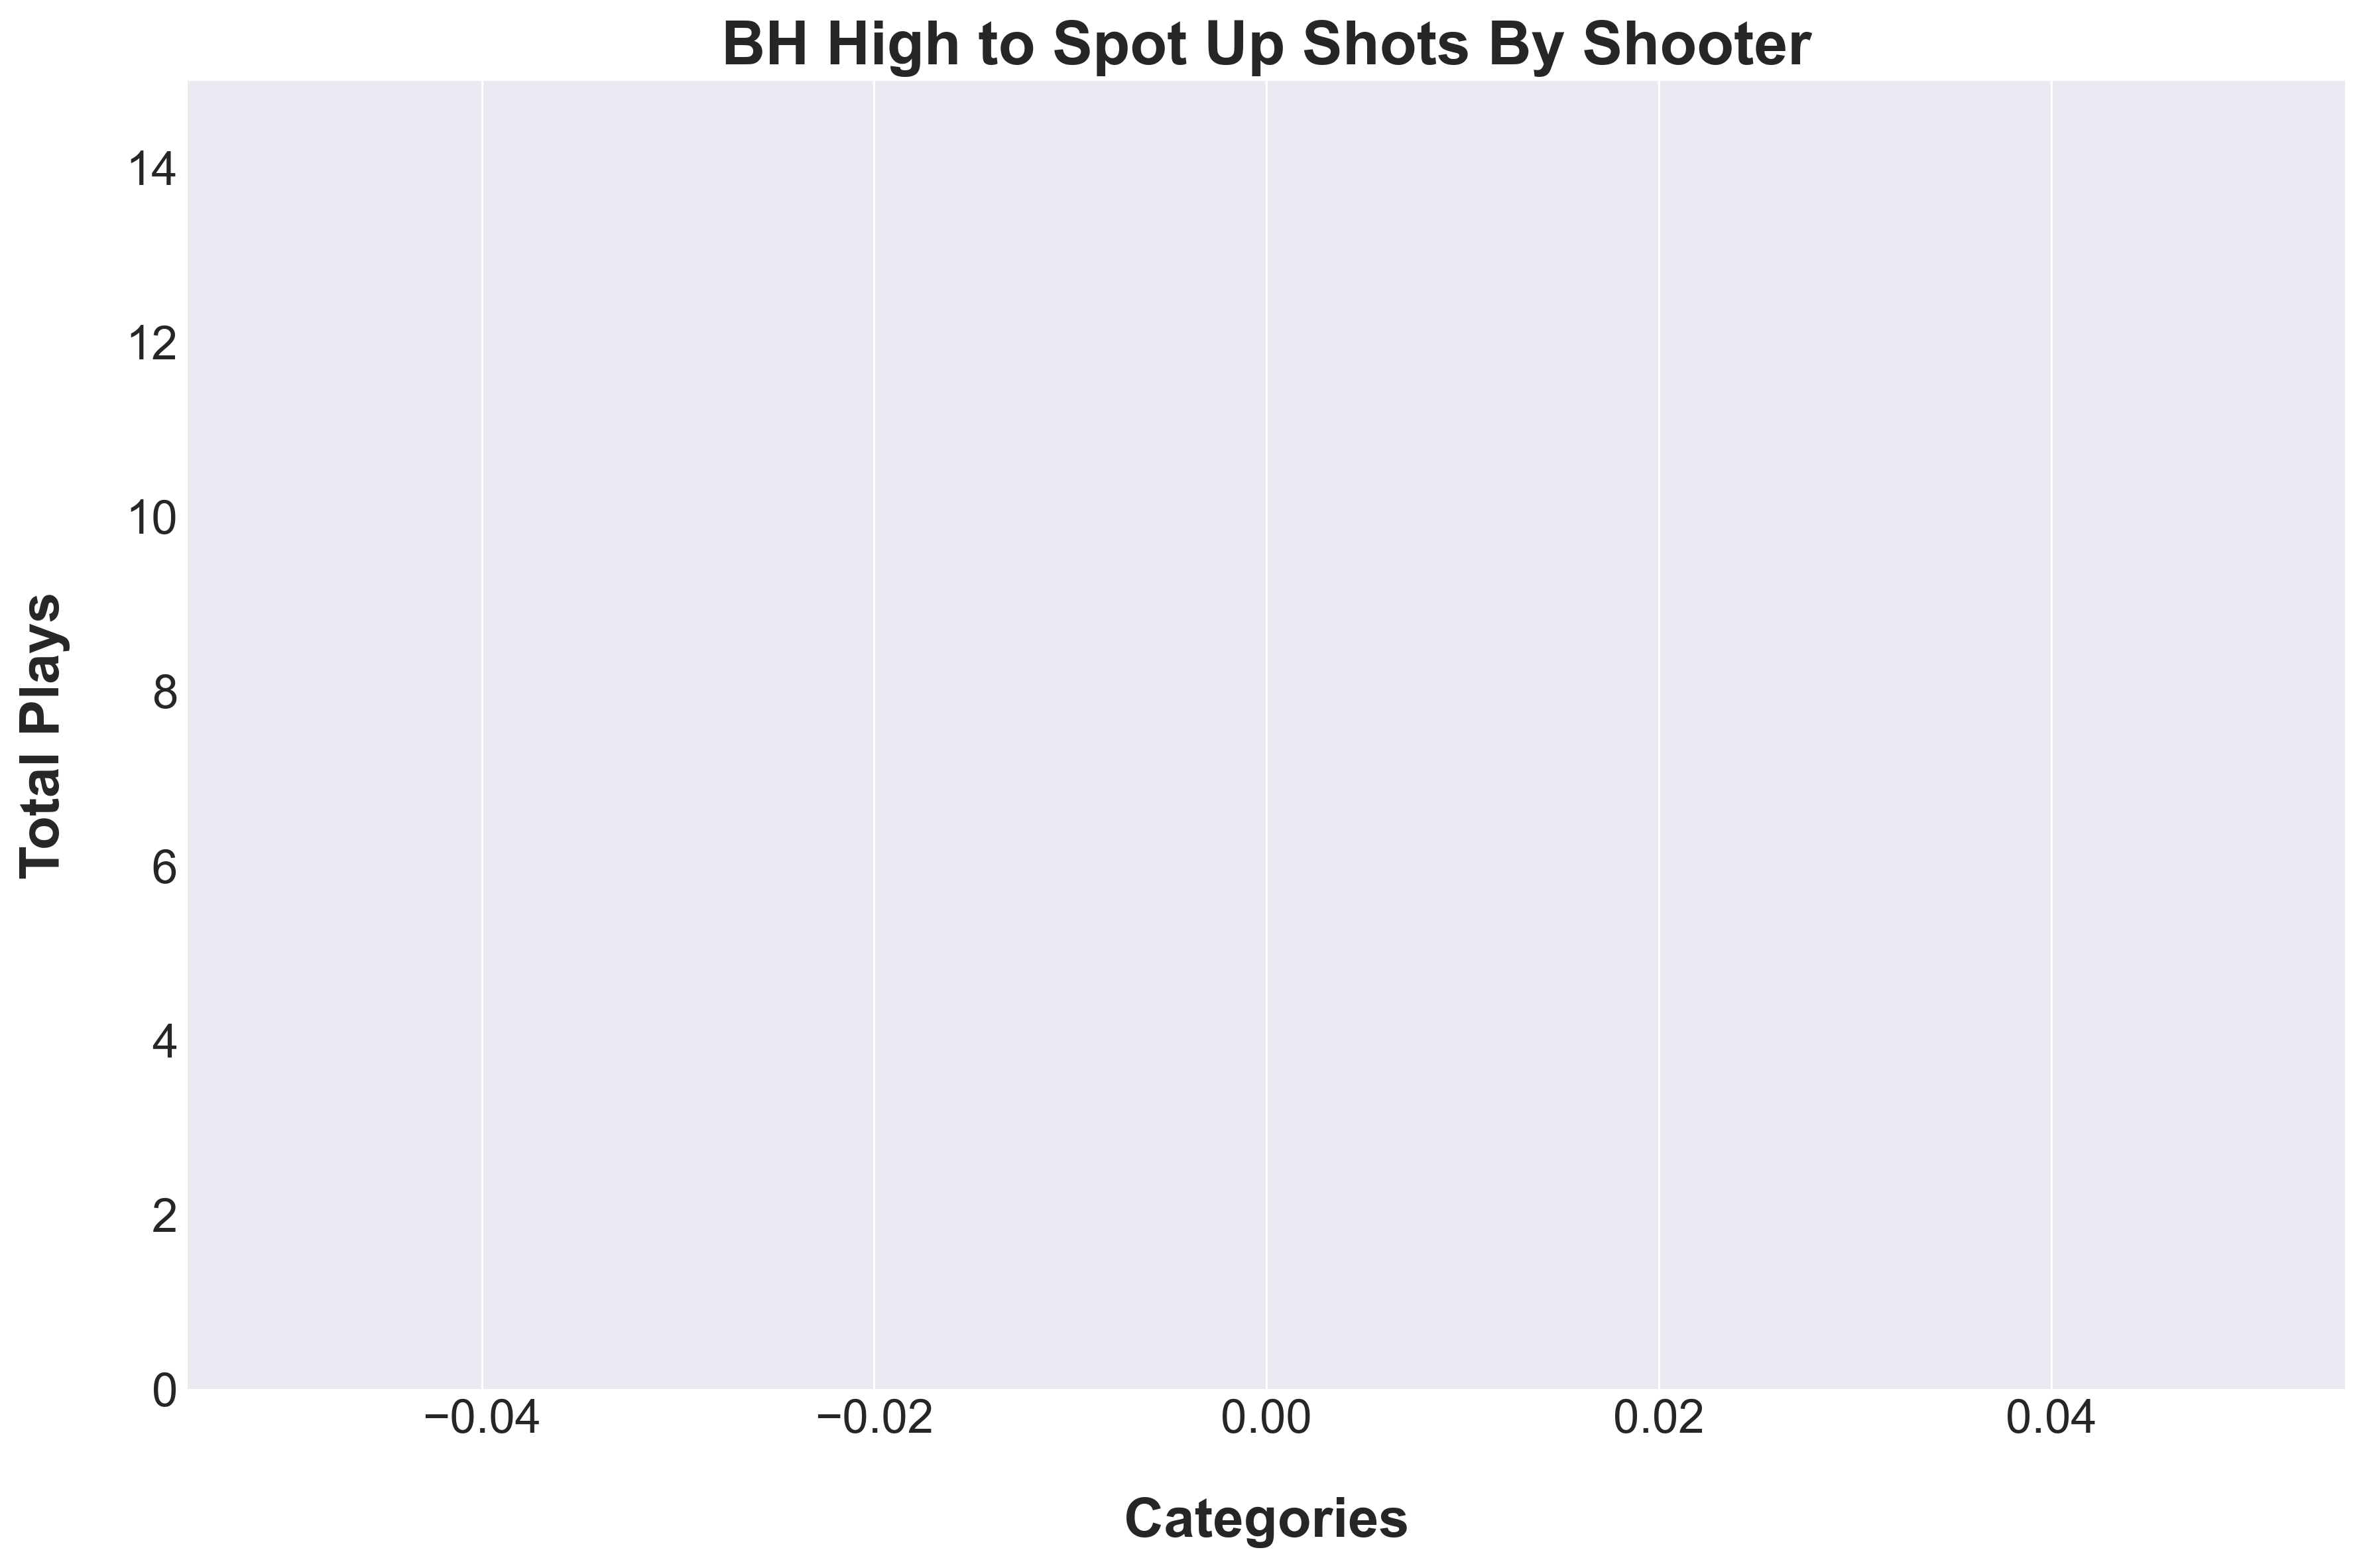
\includegraphics[width=\textwidth, height=.14\textheight]{images/PNR_PassHighShotsPlayer_Freq.png} % Adjust the width of the image to fit
    \end{minipage}
\end{table}

\vspace{-1em} % Add vertical space before the line (optional)
%\hrule height 1pt width 1\textwidth % Adjust height and width
\vspace{-1em} % Add vertical space after the line (optional)

% BH High -> Rollman Rolls Secondary Player Stats
\begin{table}[H]
    \raisebox{3em}{ % Adjust this value to shift the tables vertically
    \begin{minipage}[t]{0.6\textwidth} % Left side (table) takes 85% of the width
        \flushleft
        \centering % Centering the title and the table
        \text{BH High - Rollman Rolls Player Statistics} % Title above the table in bold
        \vskip .25em % Adds vertical space between title and table
        \scalebox{.6}{ % Scale the entire table down by half
            \renewcommand{\arraystretch}{1.4} % Adjust the number to increase or decrease row spacing
            \begin{tabular}{
            >{\centering\arraybackslash}p{3cm} 
            >{\centering\arraybackslash}p{.75cm} 
            >{\centering\arraybackslash}p{.75cm} 
            >{\centering\arraybackslash}p{.75cm} 
            >{\centering\arraybackslash}p{.75cm}
            >{\centering\arraybackslash}p{.75cm} 
            >{\centering\arraybackslash}p{.75cm}
            >{\centering\arraybackslash}p{.75cm}
            >{\centering\arraybackslash}p{.75cm} 
            >{\centering\arraybackslash}p{.75cm}}% Adjust column widths
            \toprule
            {\scriptsize \textbf{Player}} &
            {\scriptsize \textbf{Plays}} &
            {\scriptsize \textbf{2PA}} & 
            {\scriptsize \textbf{2PM}} & 
            {\scriptsize \textbf{2P\%}} & 
            {\scriptsize \textbf{MiA}} & 
            {\scriptsize \textbf{MiM}} &
            {\scriptsize \textbf{Mi\%}} &
            {\scriptsize \textbf{TO}} &
            {\scriptsize \textbf{Foul}} \\
            \midrule
            
                
            
                
            
                
            
                
            
                
            
                
            
                
            
                
            
                
            
                
                    
                        Josiah Turner & 
                        1 & 
                        1 & 
                        1 & 
                        100.0 & 
                        0 & 
                        0 & 
                        - & 
                        0 & 
                        0 \\
                    
                        Kenny Wilburn & 
                        1 & 
                        1 & 
                        0 & 
                        0.0 & 
                        0 & 
                        0 & 
                        - & 
                        0 & 
                        0 \\
                    
                
            
                
            
                
            
                
            
                
            
                
            
                
            
                
            
                
            
                
            
                
            
                
            
                
            
                
            
                
            
                
            
                
            
                
            
                
            
                
            
                
            
                
            
                
            
                
            
                
            
                
            
                
            
                
            
                
            

            \bottomrule
        \end{tabular}
        } % End of \scalebox
    \end{minipage}
    } % End of raisebox, closing the adjustment
    \hfill % This adds some flexible space between the table and the image
    \begin{minipage}[c]{0.35\textwidth} % Right side (image) takes 10% of the width
        \flushright
        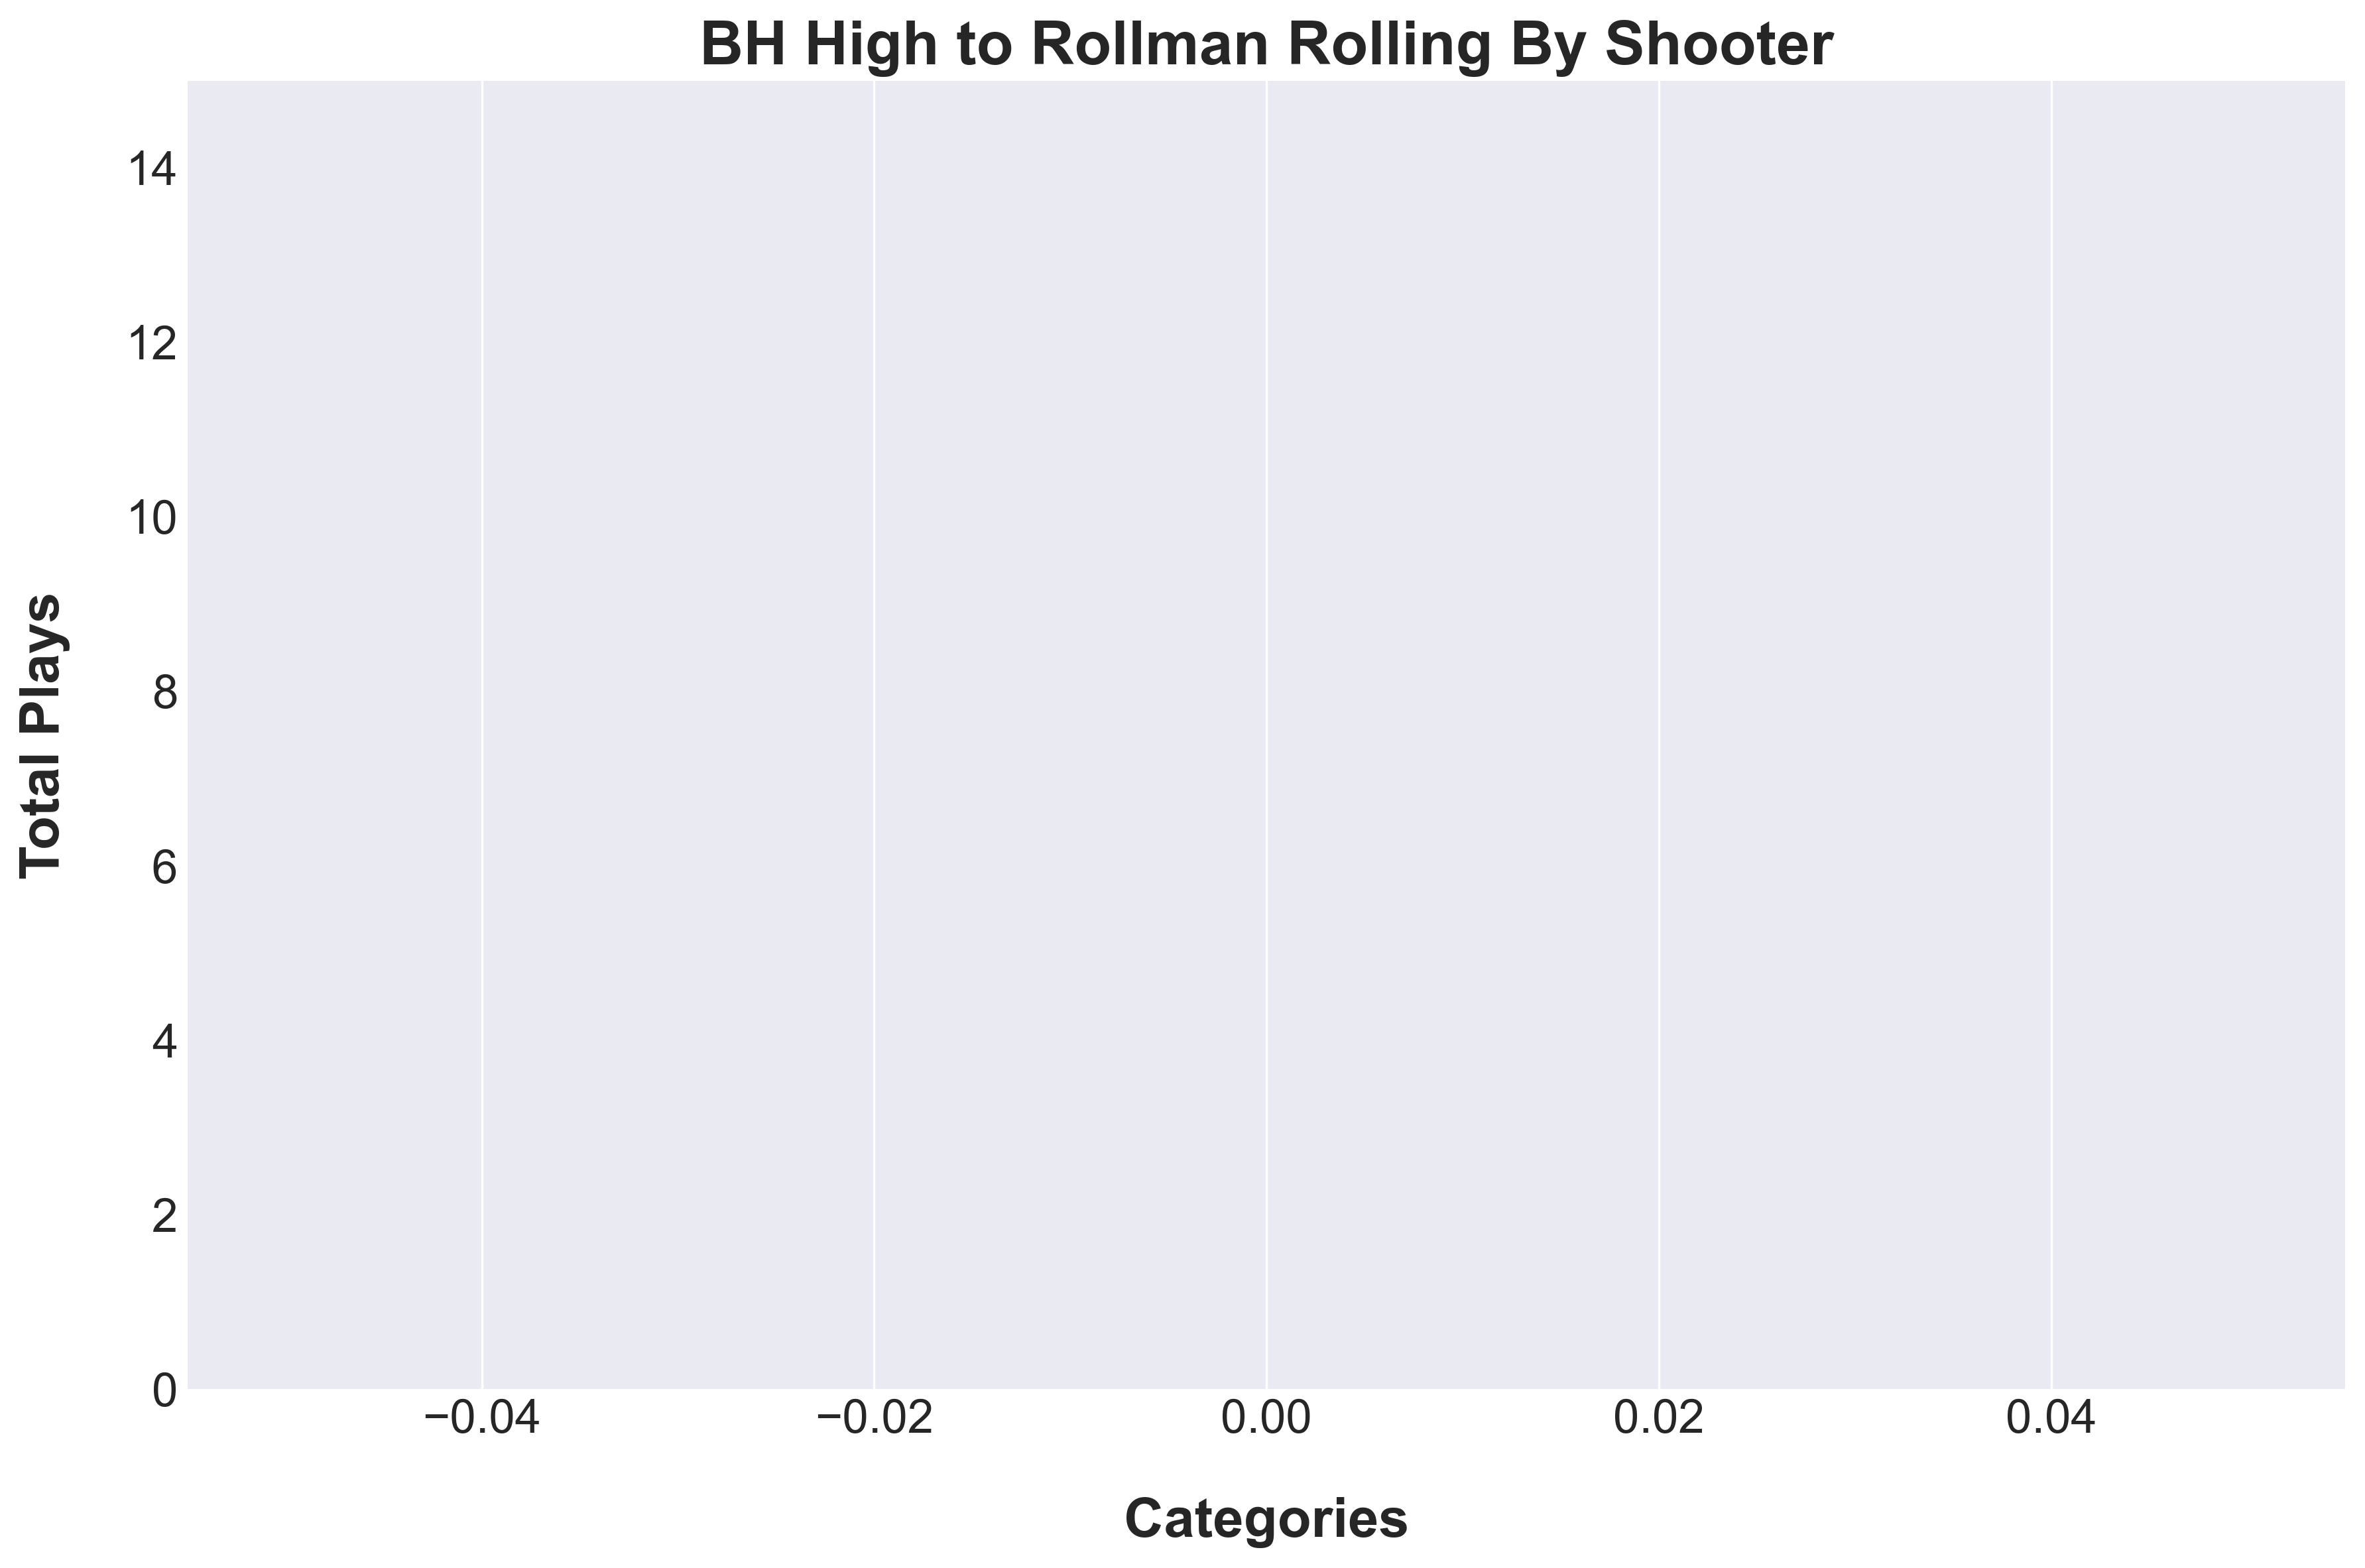
\includegraphics[width=\textwidth, height=.14\textheight]{images/PNR_PassHighRollsPlayer_Freq.png} % Adjust the width of the image to fit
    \end{minipage}
\end{table}

\vspace{-1em} % Add vertical space before the line (optional)
%\hrule height 1pt width 1\textwidth % Adjust height and width
\vspace{-1em} % Add vertical space after the line (optional)

% BH High -> Rollman Slips Secondary Player Stats
\begin{table}[H]
    \raisebox{3em}{ % Adjust this value to shift the tables vertically
    \begin{minipage}[t]{0.6\textwidth} % Left side (table) takes 85% of the width
        \flushleft
        \centering % Centering the title and the table
        \text{BH High - Rollman Slips Player Statistics} % Title above the table in bold
        \vskip .25em % Adds vertical space between title and table
        \scalebox{.55}{ % Scale the entire table down by half
            \renewcommand{\arraystretch}{1.4} % Adjust the number to increase or decrease row spacing
            \begin{tabular}{
            >{\centering\arraybackslash}p{3cm} 
            >{\centering\arraybackslash}p{.75cm} 
            >{\centering\arraybackslash}p{.75cm} 
            >{\centering\arraybackslash}p{.75cm} 
            >{\centering\arraybackslash}p{.75cm}
            >{\centering\arraybackslash}p{.75cm} 
            >{\centering\arraybackslash}p{.75cm} 
            >{\centering\arraybackslash}p{.75cm} 
            >{\centering\arraybackslash}p{.75cm}
            >{\centering\arraybackslash}p{.75cm} 
            >{\centering\arraybackslash}p{.75cm}
            >{\centering\arraybackslash}p{.75cm} 
            >{\centering\arraybackslash}p{.75cm}}% Adjust column widths
            \toprule
            {\scriptsize \textbf{Player}} &
            {\scriptsize \textbf{Plays}} &
            {\scriptsize \textbf{3PA}} &
            {\scriptsize \textbf{3PM}} &
            {\scriptsize \textbf{3P\%}} & 
            {\scriptsize \textbf{2PA}} & 
            {\scriptsize \textbf{2PM}} & 
            {\scriptsize \textbf{2P\%}} & 
            {\scriptsize \textbf{MiA}} & 
            {\scriptsize \textbf{MiM}} &
            {\scriptsize \textbf{Mi\%}} &
            {\scriptsize \textbf{TO}} &
            {\scriptsize \textbf{Foul}} \\
            \midrule
            
                
            
                
            
                
            
                
            
                
            
                
            
                
            
                
            
                
            
                
            
                
                    
                        Kenny Wilburn & 
                        1 & 
                        1 & 
                        0 & 
                        0.0 & 
                        0 & 
                        0 & 
                        - & 
                        0 & 
                        0 & 
                        - & 
                        0 & 
                        0 \\
                    
                
            
                
            
                
            
                
            
                
            
                
            
                
            
                
            
                
            
                
            
                
            
                
            
                
            
                
            
                
            
                
            
                
            
                
            
                
            
                
            
                
            
                
            
                
            
                
            
                
            
                
            
                
            
                
            

            \bottomrule
        \end{tabular}
        } % End of \scalebox
    \end{minipage}
    } % End of raisebox, closing the adjustment
    \hfill % This adds some flexible space between the table and the image
    \begin{minipage}[c]{0.35\textwidth} % Right side (image) takes 10% of the width
        \flushright
        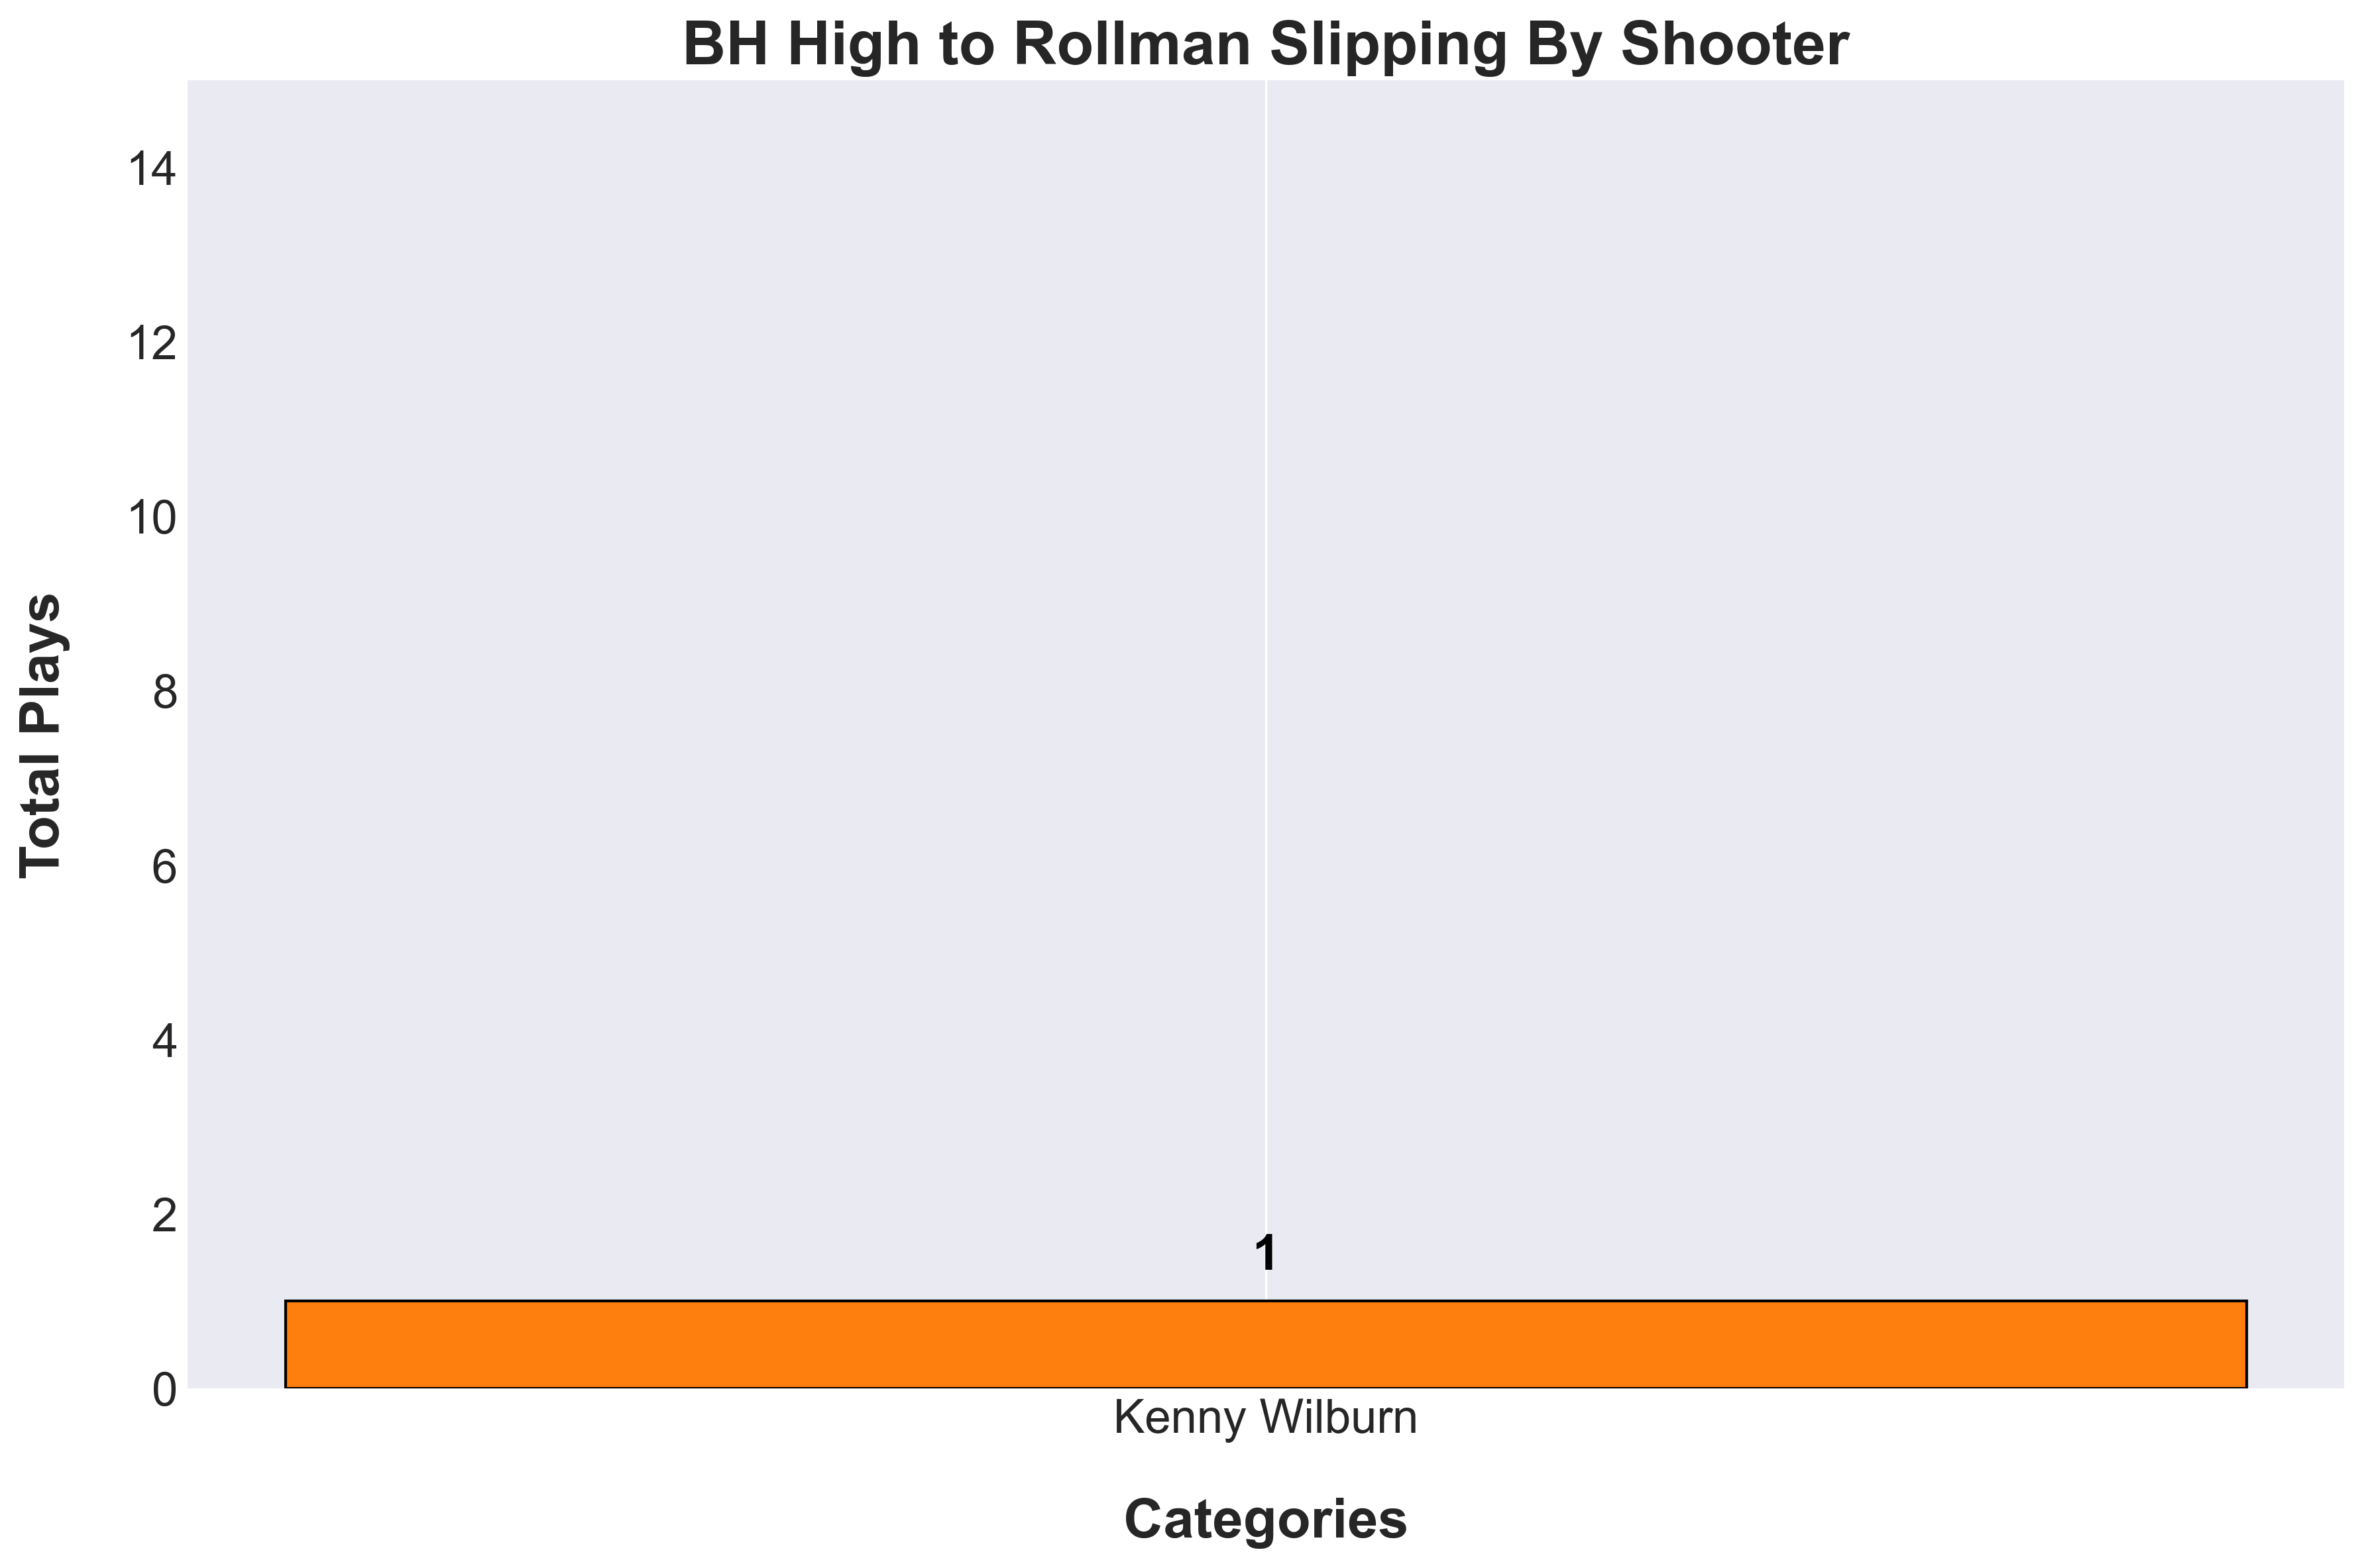
\includegraphics[width=\textwidth, height=.14\textheight]{images/PNR_PassHighSlipsPlayer_Freq.png} % Adjust the width of the image to fit
    \end{minipage}
\end{table}

\vspace{-1em} % Add vertical space before the line (optional)
%\hrule height 1pt width 1\textwidth % Adjust height and width
\vspace{-1em} % Add vertical space after the line (optional)

% BH High -> Rollman Pops Secondary Player Stats
\begin{table}[H]
    \raisebox{3em}{ % Adjust this value to shift the tables vertically
    \begin{minipage}[t]{0.6\textwidth} % Left side (table) takes 85% of the width
        \flushleft
        \centering % Centering the title and the table
        \text{BH High - Rollman Pops Player Statistics} % Title above the table in bold
        \vskip .25em % Adds vertical space between title and table
        \scalebox{.55}{ % Scale the entire table down by half
            \renewcommand{\arraystretch}{1.4} % Adjust the number to increase or decrease row spacing
            \begin{tabular}{
            >{\centering\arraybackslash}p{3cm} 
            >{\centering\arraybackslash}p{.75cm} 
            >{\centering\arraybackslash}p{.75cm} 
            >{\centering\arraybackslash}p{.75cm} 
            >{\centering\arraybackslash}p{.75cm}
            >{\centering\arraybackslash}p{.75cm} 
            >{\centering\arraybackslash}p{.75cm} 
            >{\centering\arraybackslash}p{.75cm} 
            >{\centering\arraybackslash}p{.75cm}
            >{\centering\arraybackslash}p{.75cm} 
            >{\centering\arraybackslash}p{.75cm}
            >{\centering\arraybackslash}p{.75cm} 
            >{\centering\arraybackslash}p{.75cm}}% Adjust column widths
            \toprule
            {\scriptsize \textbf{Player}} &
            {\scriptsize \textbf{Plays}} &
            {\scriptsize \textbf{3PA}} &
            {\scriptsize \textbf{3PM}} &
            {\scriptsize \textbf{3P\%}} & 
            {\scriptsize \textbf{2PA}} & 
            {\scriptsize \textbf{2PM}} & 
            {\scriptsize \textbf{2P\%}} & 
            {\scriptsize \textbf{MiA}} & 
            {\scriptsize \textbf{MiM}} &
            {\scriptsize \textbf{Mi\%}} &
            {\scriptsize \textbf{TO}} &
            {\scriptsize \textbf{Foul}} \\
            \midrule
            
                
            
                
            
                
            
                
            
                
            
                
            
                
            
                
            
                
            
                
            
                
            
                
                    
                        Josiah Turner & 
                        6 & 
                        3 & 
                        0 & 
                        0.0 & 
                        2 & 
                        0 & 
                        0.0 & 
                        0 & 
                        0 & 
                        - & 
                        0 & 
                        1 \\
                    
                        Kenny Wilburn & 
                        2 & 
                        2 & 
                        1 & 
                        50.0 & 
                        0 & 
                        0 & 
                        - & 
                        0 & 
                        0 & 
                        - & 
                        0 & 
                        0 \\
                    
                
            
                
            
                
            
                
            
                
            
                
            
                
            
                
            
                
            
                
            
                
            
                
            
                
            
                
            
                
            
                
            
                
            
                
            
                
            
                
            
                
            
                
            
                
            
                
            
                
            
                
            
                
            

            \bottomrule
        \end{tabular}
        } % End of \scalebox
    \end{minipage}
    } % End of raisebox, closing the adjustment
    \hfill % This adds some flexible space between the table and the image
    \begin{minipage}[c]{0.35\textwidth} % Right side (image) takes 10% of the width
        \flushright
        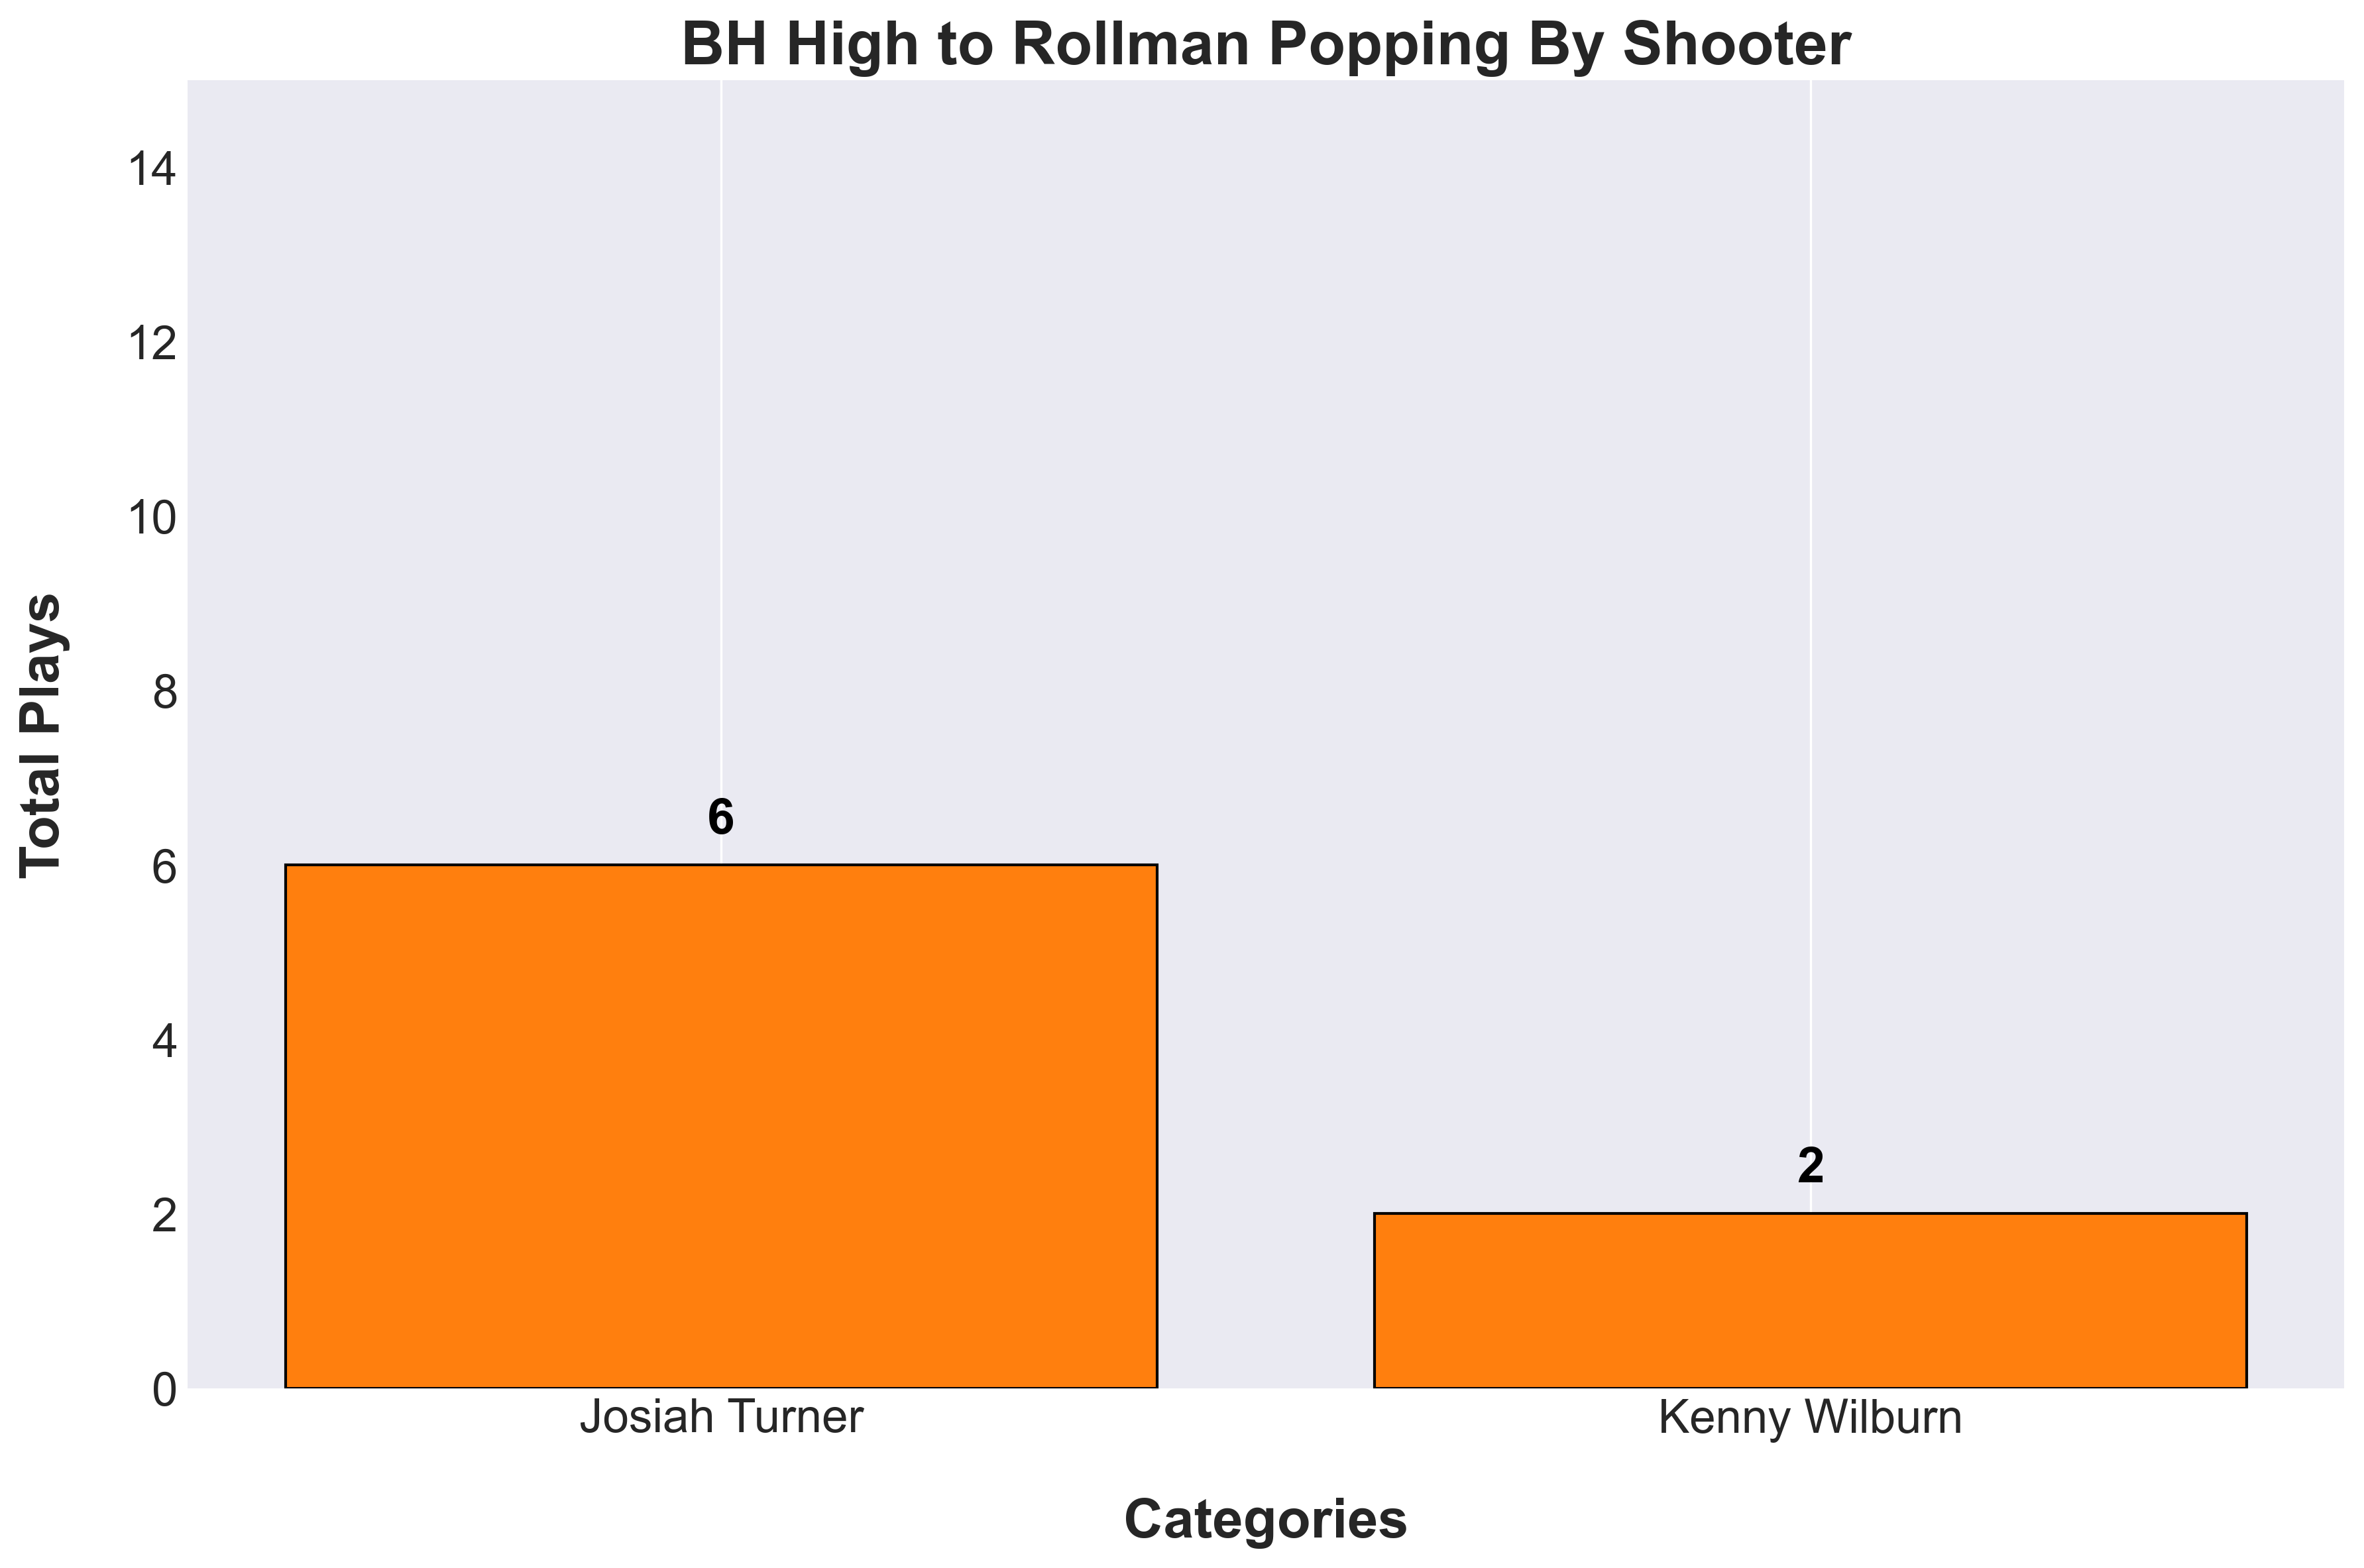
\includegraphics[width=\textwidth, height=.14\textheight]{images/PNR_PassHighPopsPlayer_Freq.png} % Adjust the width of the image to fit
    \end{minipage}
\end{table}

\vspace{-1em} % Add vertical space before the line (optional)
\hrule height 1pt width 1\textwidth % Adjust height and width
\vspace{1 em} % Add vertical space after the line (optional)

\subsubsection{BH Left PNR Passer Statistics}

% BH Left -> Cuts Secondary Player Stats
\begin{table}[H]
    \raisebox{3em}{ % Adjust this value to shift the tables vertically
    \begin{minipage}[t]{0.6\textwidth} % Left side (table) takes 85% of the width
        \flushleft
        \centering % Centering the title and the table
        \text{BH Left - Cuts Player Statistics} % Title above the table in bold
        \vskip .25em % Adds vertical space between title and table
        \scalebox{.6}{ % Scale the entire table down by half
            \renewcommand{\arraystretch}{1.4} % Adjust the number to increase or decrease row spacing
            \begin{tabular}{
            >{\centering\arraybackslash}p{3cm} 
            >{\centering\arraybackslash}p{.75cm} 
            >{\centering\arraybackslash}p{.75cm} 
            >{\centering\arraybackslash}p{.75cm} 
            >{\centering\arraybackslash}p{.75cm}
            >{\centering\arraybackslash}p{.75cm} 
            >{\centering\arraybackslash}p{.75cm}
            >{\centering\arraybackslash}p{.75cm}
            >{\centering\arraybackslash}p{.75cm} 
            >{\centering\arraybackslash}p{.75cm}}% Adjust column widths
            \toprule
            {\scriptsize \textbf{Player}} &
            {\scriptsize \textbf{Plays}} &
            {\scriptsize \textbf{2PA}} & 
            {\scriptsize \textbf{2PM}} & 
            {\scriptsize \textbf{2P\%}} & 
            {\scriptsize \textbf{MiA}} & 
            {\scriptsize \textbf{MiM}} &
            {\scriptsize \textbf{Mi\%}} &
            {\scriptsize \textbf{TO}} &
            {\scriptsize \textbf{Foul}} \\
            \midrule
            
                
            
                
            
                
            
                
            
                
            
                
            
                
            
                
            
                
            
                
            
                
            
                
            
                
                    
                
            
                
            
                
            
                
            
                
            
                
            
                
            
                
            
                
            
                
            
                
            
                
            
                
            
                
            
                
            
                
            
                
            
                
            
                
            
                
            
                
            
                
            
                
            
                
            
                
            
                
            

            \bottomrule
        \end{tabular}
        } % End of \scalebox
    \end{minipage}
    } % End of raisebox, closing the adjustment
    \hfill % This adds some flexible space between the table and the image
    \begin{minipage}[c]{0.35\textwidth} % Right side (image) takes 10% of the width
        \flushright
        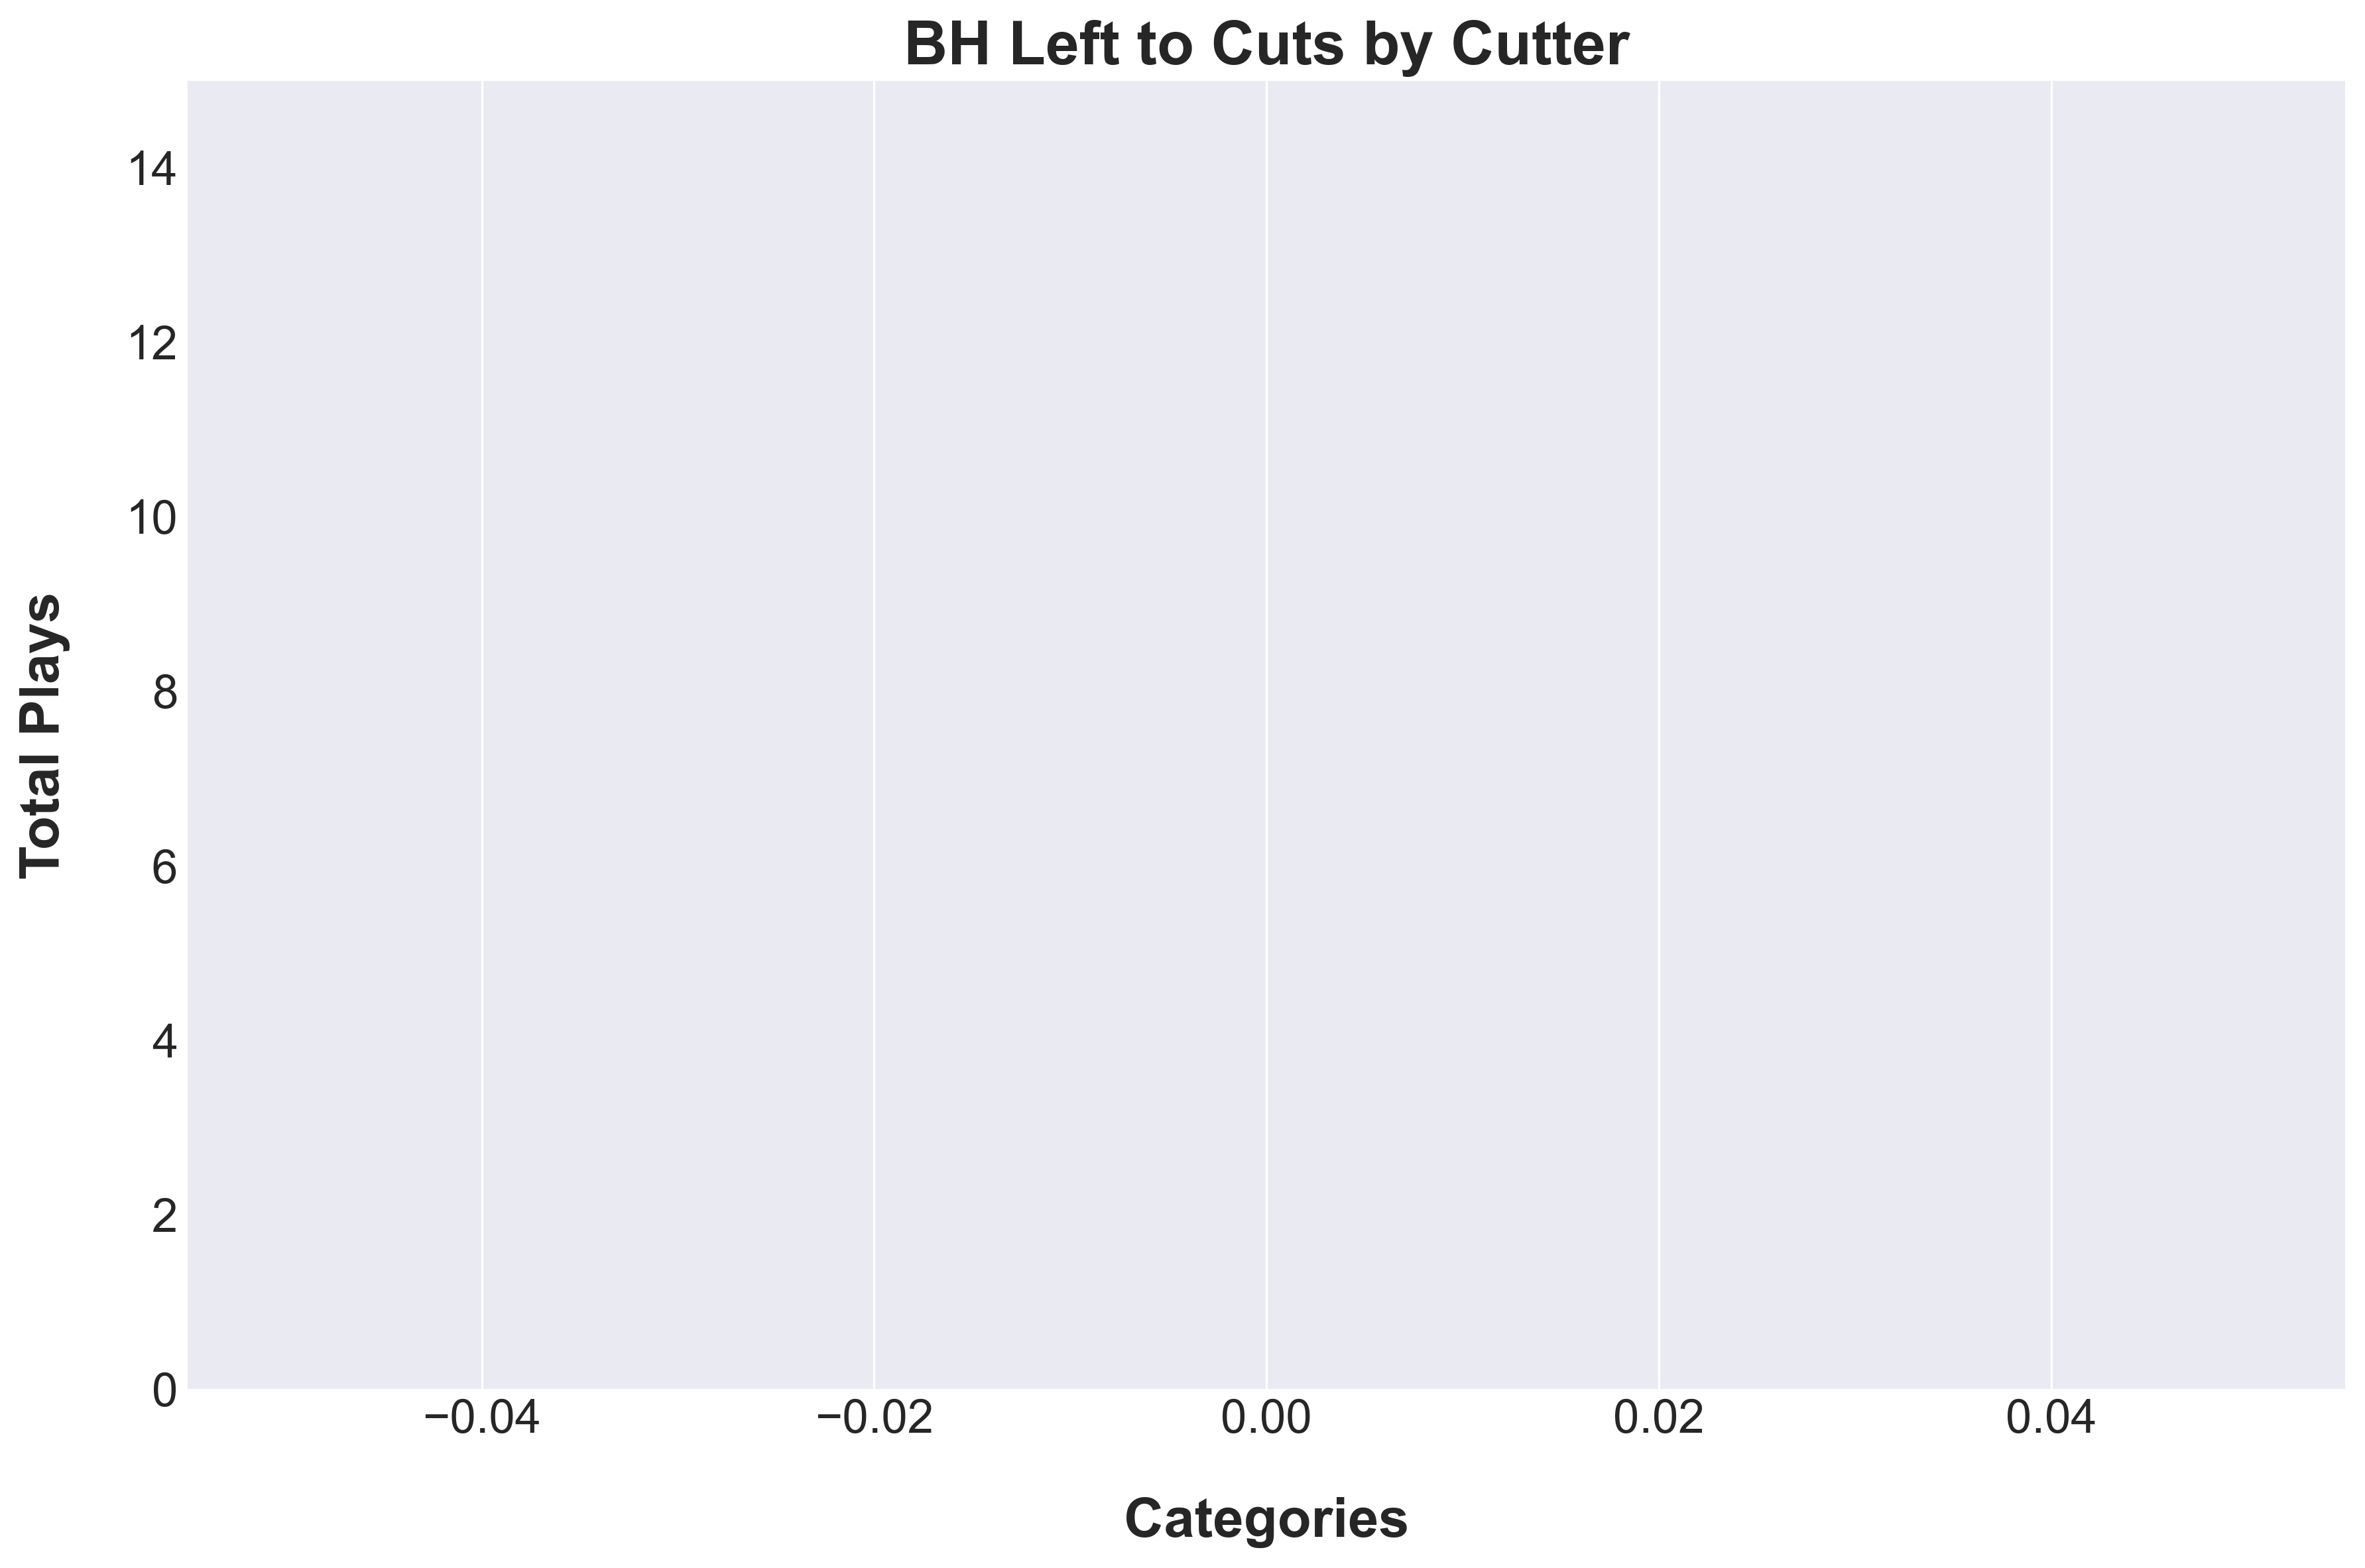
\includegraphics[width=\textwidth, height=.14\textheight]{images/PNR_PassLeftCutsPlayer_Freq.png} % Adjust the width of the image to fit
    \end{minipage}
\end{table}

\vspace{-1em} % Add vertical space before the line (optional)
%\hrule height 1pt width 1\textwidth % Adjust height and width
\vspace{-1em} % Add vertical space after the line (optional)

% BH Left -> Spot Up Drives Secondary Player Stats
\begin{table}[H]
    \raisebox{3em}{ % Adjust this value to shift the tables vertically
    \begin{minipage}[t]{0.6\textwidth} % Left side (table) takes 85% of the width
        \flushleft
        \centering % Centering the title and the table
        \text{BH Left - Spot Up Drives Player Statistics} % Title above the table in bold
        \vskip .25em % Adds vertical space between title and table
        \scalebox{.55}{ % Scale the entire table down by half
            \renewcommand{\arraystretch}{1.4} % Adjust the number to increase or decrease row spacing
            \begin{tabular}{
            >{\centering\arraybackslash}p{3cm} 
            >{\centering\arraybackslash}p{.75cm} 
            >{\centering\arraybackslash}p{.75cm} 
            >{\centering\arraybackslash}p{.75cm} 
            >{\centering\arraybackslash}p{.75cm}
            >{\centering\arraybackslash}p{.75cm} 
            >{\centering\arraybackslash}p{.75cm} 
            >{\centering\arraybackslash}p{.75cm} 
            >{\centering\arraybackslash}p{.75cm}
            >{\centering\arraybackslash}p{.75cm} 
            >{\centering\arraybackslash}p{.75cm}
            >{\centering\arraybackslash}p{.75cm} 
            >{\centering\arraybackslash}p{.75cm}}% Adjust column widths
            \toprule
            {\scriptsize \textbf{Player}} &
            {\scriptsize \textbf{Plays}} &
            {\scriptsize \textbf{3PA}} &
            {\scriptsize \textbf{3PM}} &
            {\scriptsize \textbf{3P\%}} & 
            {\scriptsize \textbf{2PA}} & 
            {\scriptsize \textbf{2PM}} & 
            {\scriptsize \textbf{2P\%}} & 
            {\scriptsize \textbf{MiA}} & 
            {\scriptsize \textbf{MiM}} &
            {\scriptsize \textbf{Mi\%}} &
            {\scriptsize \textbf{TO}} &
            {\scriptsize \textbf{Foul}} \\
            \midrule
            
                
            
                
            
                
            
                
            
                
            
                
            
                
            
                
            
                
            
                
            
                
            
                
            
                
            
                
                    
                        Ronnie Toole & 
                        1 & 
                        0 & 
                        0 & 
                        - & 
                        1 & 
                        0 & 
                        0.0 & 
                        0 & 
                        0 & 
                        - & 
                        0 & 
                        0 \\
                    
                        Zac Ditzel & 
                        1 & 
                        0 & 
                        0 & 
                        - & 
                        1 & 
                        0 & 
                        0.0 & 
                        0 & 
                        0 & 
                        - & 
                        0 & 
                        0 \\
                    
                
            
                
            
                
            
                
            
                
            
                
            
                
            
                
            
                
            
                
            
                
            
                
            
                
            
                
            
                
            
                
            
                
            
                
            
                
            
                
            
                
            
                
            
                
            
                
            
                
            

            \bottomrule
        \end{tabular}
        } % End of \scalebox
    \end{minipage}
    } % End of raisebox, closing the adjustment
    \hfill % This adds some flexible space between the table and the image
    \begin{minipage}[c]{0.35\textwidth} % Right side (image) takes 10% of the width
        \flushright
        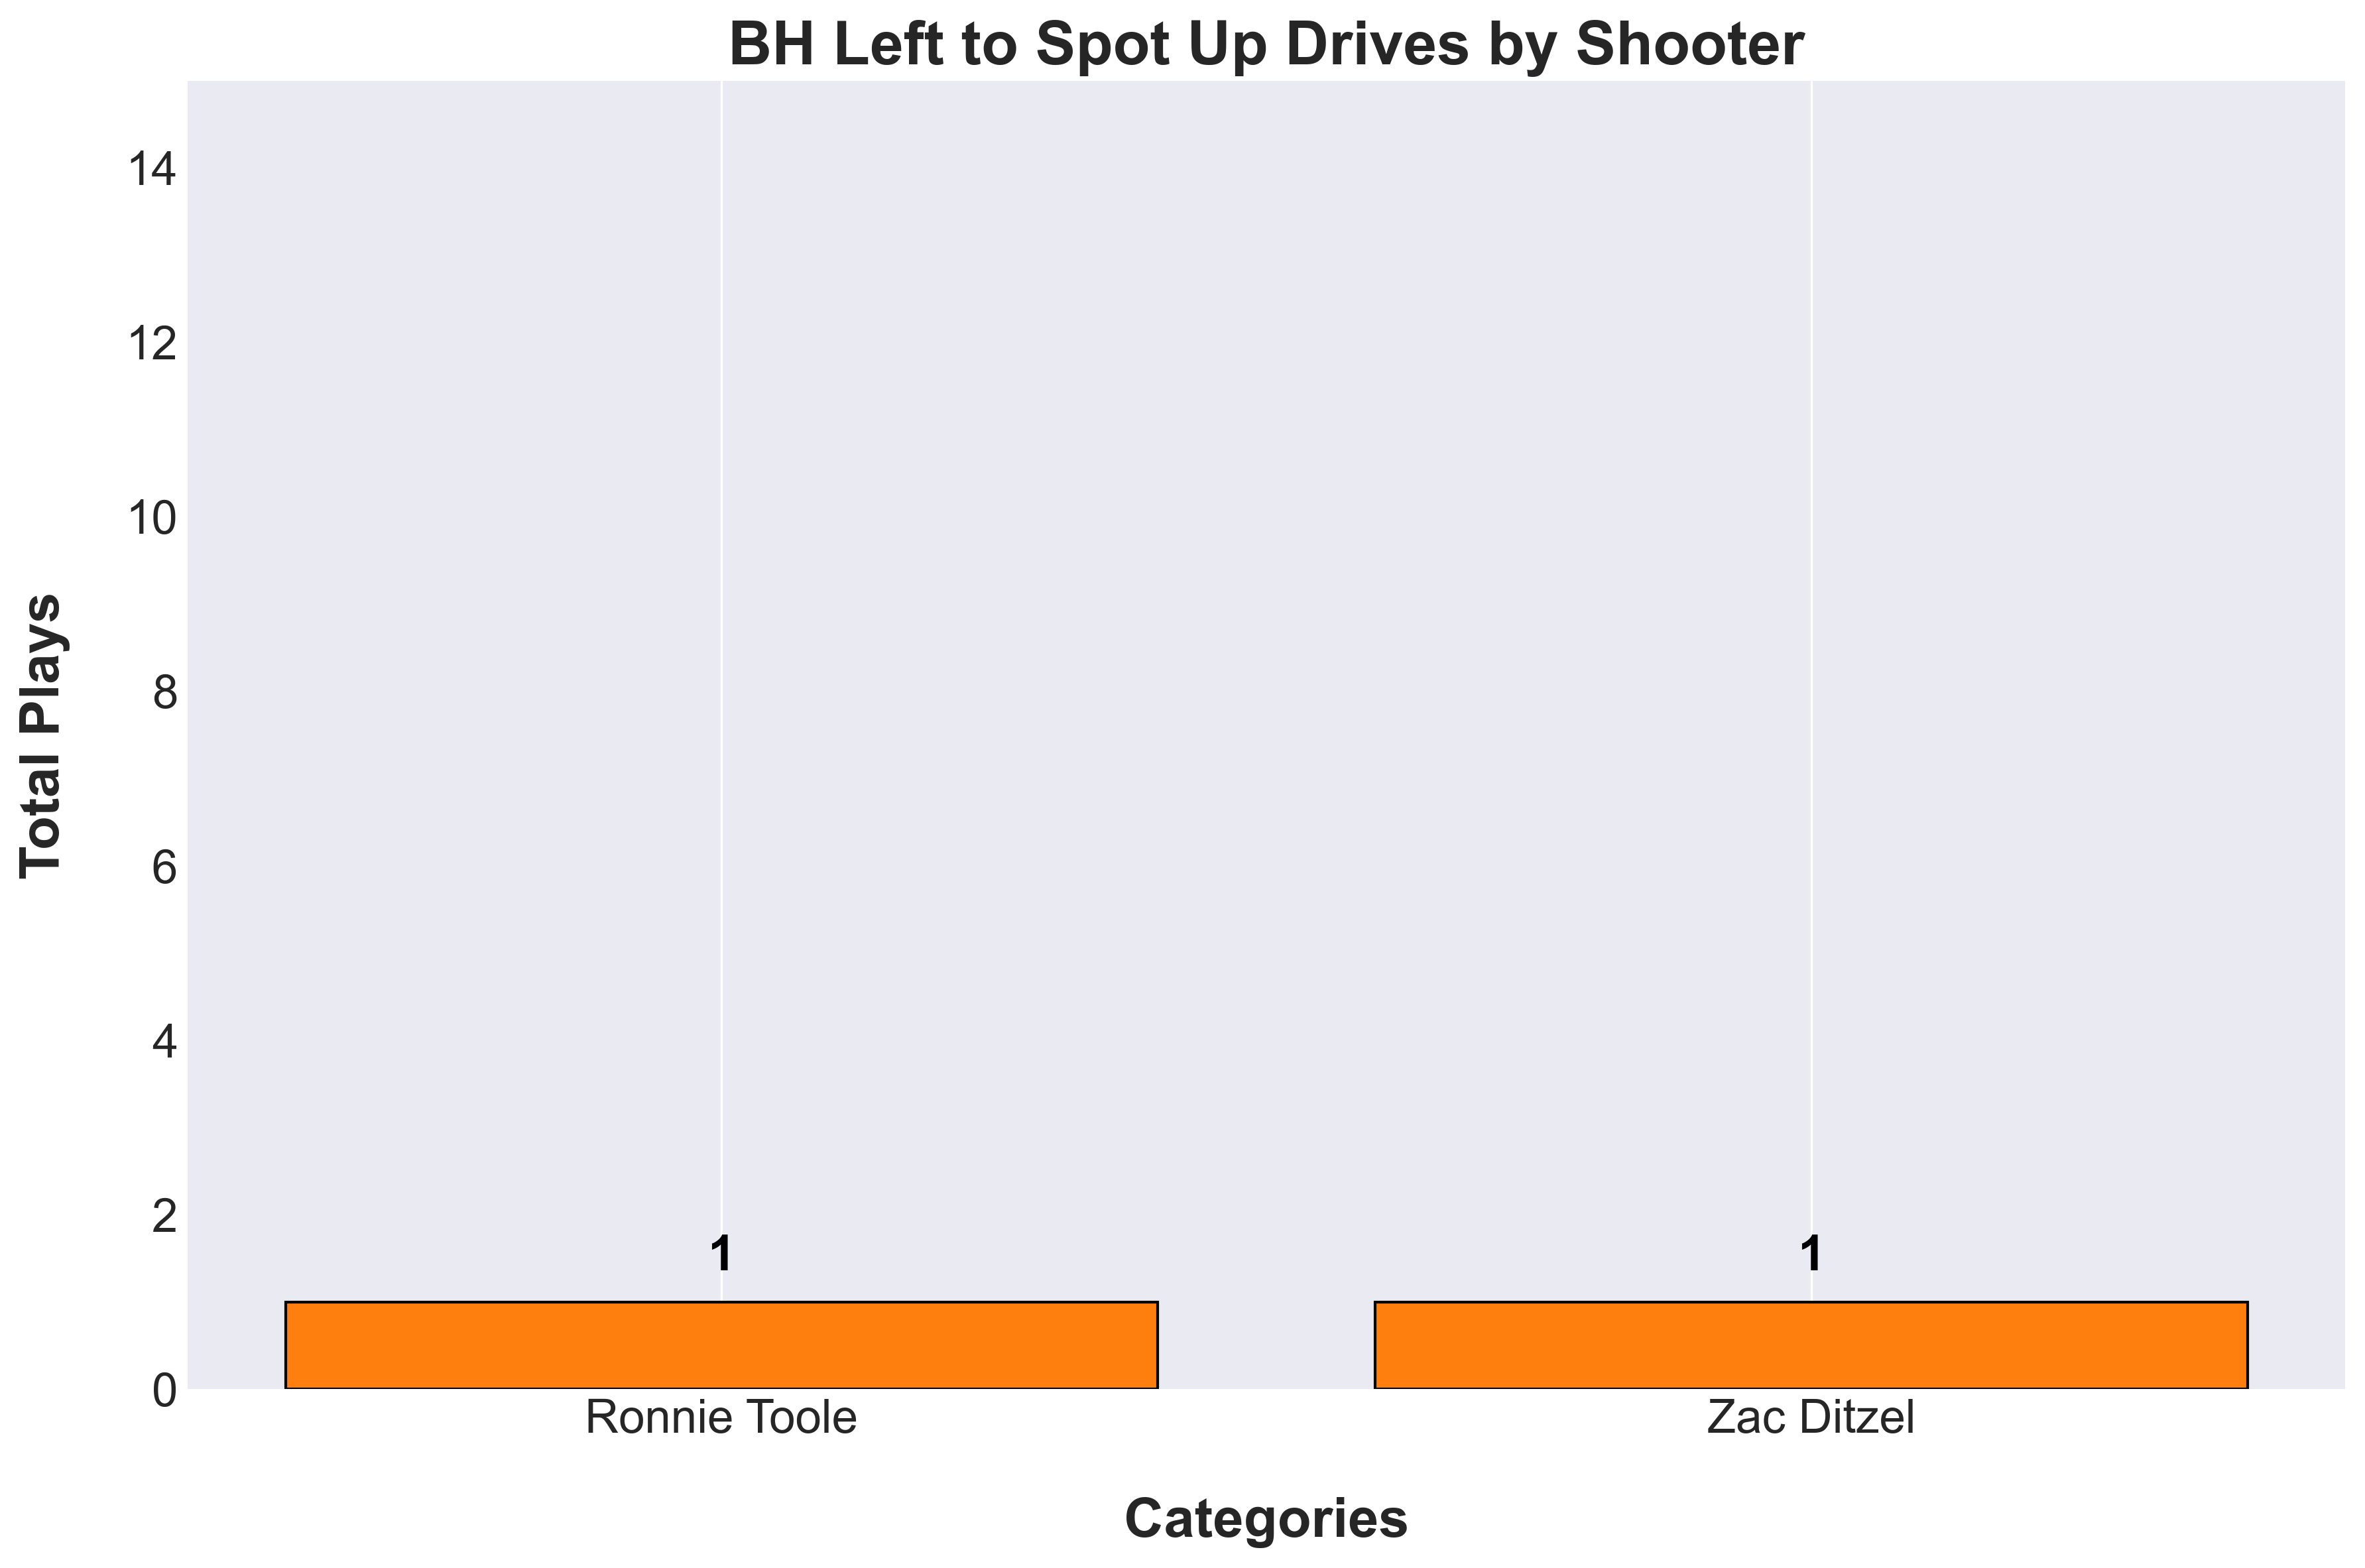
\includegraphics[width=\textwidth, height=.14\textheight]{images/PNR_PassLeftDrivesPlayer_Freq.png} % Adjust the width of the image to fit
    \end{minipage}
\end{table}

\vspace{-1em} % Add vertical space before the line (optional)
%\hrule height 1pt width 1\textwidth % Adjust height and width
\vspace{-1em} % Add vertical space after the line (optional)

% BH Left -> Spot Up Shots Secondary Player Stats
\begin{table}[H]
    \raisebox{3em}{ % Adjust this value to shift the tables vertically
    \begin{minipage}[t]{0.6\textwidth} % Left side (table) takes 85% of the width
        \flushleft
        \centering % Centering the title and the table
        \text{BH Left - Spot Up Shots Player Statistics} % Title above the table in bold
        \vskip .25em % Adds vertical space between title and table
        \scalebox{.6}{ % Scale the entire table down by half
            \renewcommand{\arraystretch}{1.4} % Adjust the number to increase or decrease row spacing
            \begin{tabular}{
            >{\centering\arraybackslash}p{3cm} 
            >{\centering\arraybackslash}p{.75cm} 
            >{\centering\arraybackslash}p{.75cm} 
            >{\centering\arraybackslash}p{.75cm} 
            >{\centering\arraybackslash}p{.75cm}
            >{\centering\arraybackslash}p{.75cm} 
            >{\centering\arraybackslash}p{.75cm} 
            >{\centering\arraybackslash}p{.75cm} 
            >{\centering\arraybackslash}p{.75cm}
            >{\centering\arraybackslash}p{.75cm} 
            >{\centering\arraybackslash}p{.75cm}
            >{\centering\arraybackslash}p{.75cm} 
            >{\centering\arraybackslash}p{.75cm}}% Adjust column widths
            \toprule
            {\scriptsize \textbf{Player}} &
            {\scriptsize \textbf{Plays}} &
            {\scriptsize \textbf{3PA}} &
            {\scriptsize \textbf{3PM}} &
            {\scriptsize \textbf{3P\%}} & 
            {\scriptsize \textbf{MiA}} & 
            {\scriptsize \textbf{MiM}} &
            {\scriptsize \textbf{Mi\%}} &
            {\scriptsize \textbf{TO}} &
            {\scriptsize \textbf{Foul}} \\
            \midrule
            
                
            
                
            
                
            
                
            
                
            
                
            
                
            
                
            
                
            
                
            
                
            
                
            
                
            
                
            
                
                    
                        Brock Bowen & 
                        1 & 
                        1 & 
                        0 & 
                        0.0 & 
                        0 & 
                        0 & 
                        - & 
                        0 & 
                        0 \\
                    
                        Brody Brown & 
                        1 & 
                        1 & 
                        0 & 
                        0.0 & 
                        0 & 
                        0 & 
                        - & 
                        0 & 
                        0 \\
                    
                        Keegan Ocorr & 
                        1 & 
                        1 & 
                        0 & 
                        0.0 & 
                        0 & 
                        0 & 
                        - & 
                        0 & 
                        0 \\
                    
                
            
                
            
                
            
                
            
                
            
                
            
                
            
                
            
                
            
                
            
                
            
                
            
                
            
                
            
                
            
                
            
                
            
                
            
                
            
                
            
                
            
                
            
                
            
                
            
            \bottomrule
        \end{tabular}
        } % End of \scalebox
    \end{minipage}
    } % End of raisebox, closing the adjustment
    \hfill % This adds some flexible space between the table and the image
    \begin{minipage}[c]{0.35\textwidth} % Right side (image) takes 10% of the width
        \flushright
        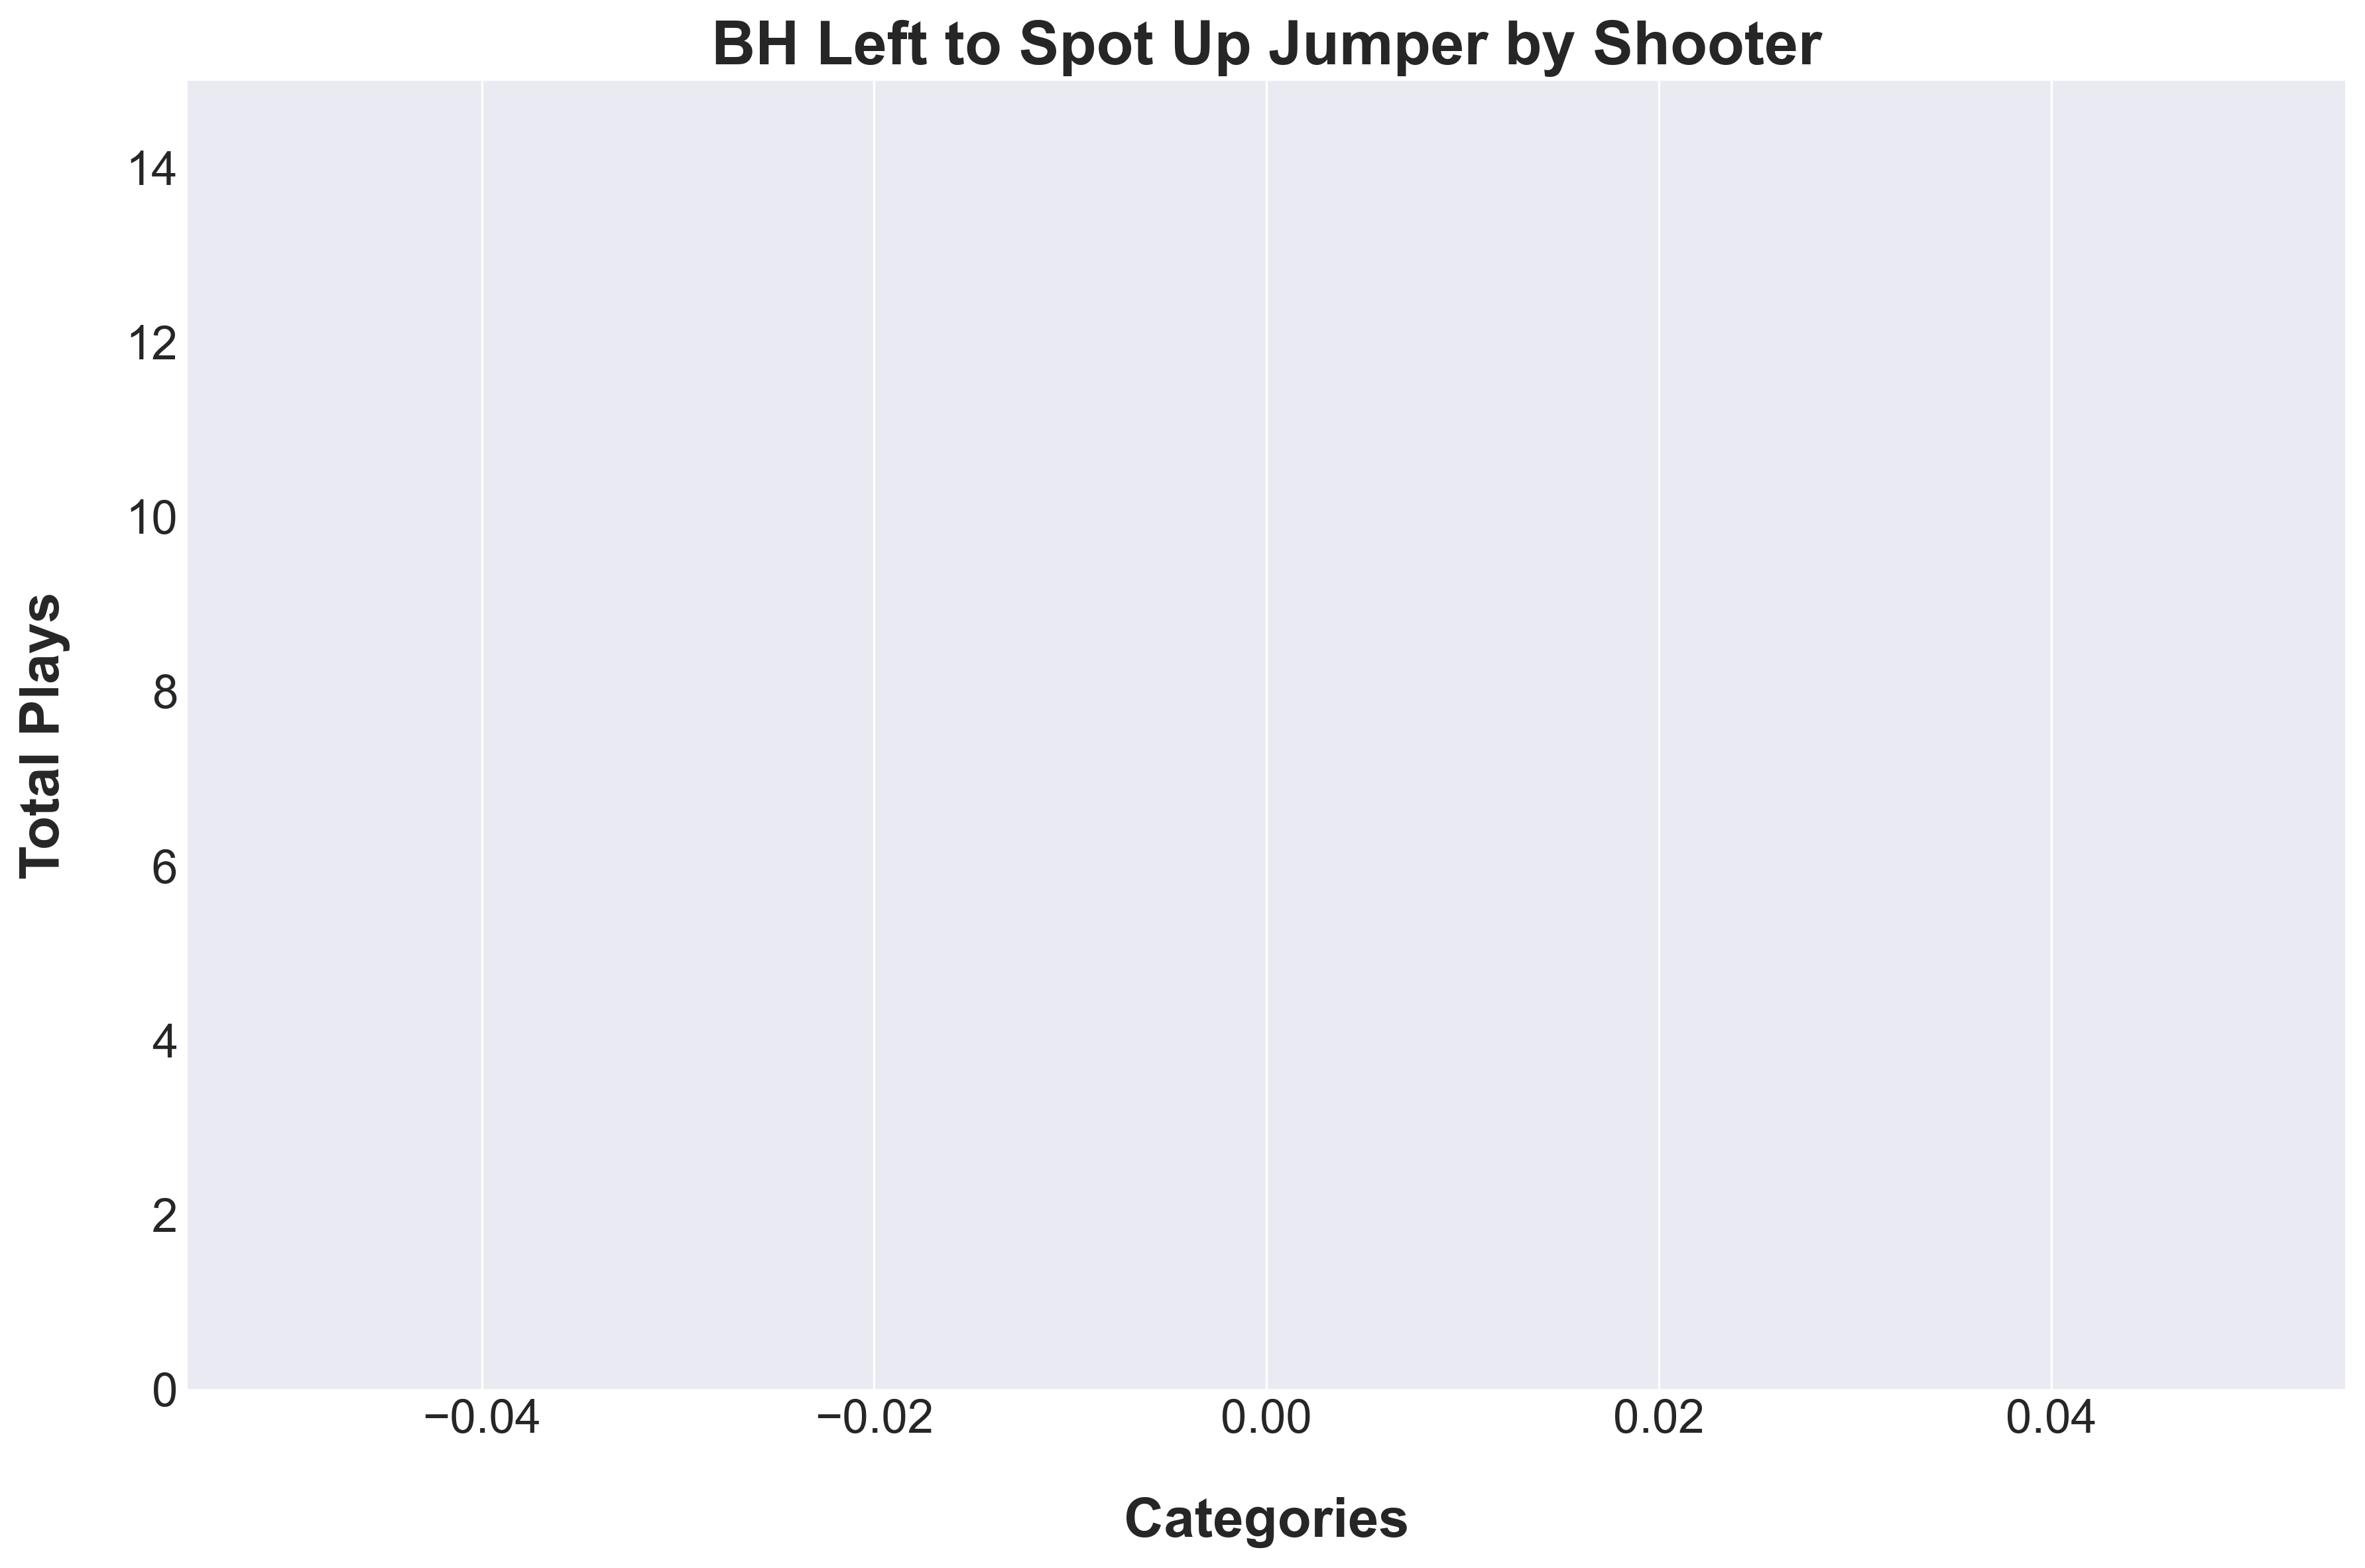
\includegraphics[width=\textwidth, height=.14\textheight]{images/PNR_PassLeftShotsPlayer_Freq.png} % Adjust the width of the image to fit
    \end{minipage}
\end{table}

\vspace{-1em} % Add vertical space before the line (optional)
%\hrule height 1pt width 1\textwidth % Adjust height and width
\vspace{-1em} % Add vertical space after the line (optional)

% BH Left -> Rollman Rolls Secondary Player Stats
\begin{table}[H]
    \raisebox{3em}{ % Adjust this value to shift the tables vertically
    \begin{minipage}[t]{0.6\textwidth} % Left side (table) takes 85% of the width
        \flushleft
        \centering % Centering the title and the table
        \text{BH Left - Rollman Rolls Player Statistics} % Title above the table in bold
        \vskip .25em % Adds vertical space between title and table
        \scalebox{.6}{ % Scale the entire table down by half
            \renewcommand{\arraystretch}{1.4} % Adjust the number to increase or decrease row spacing
            \begin{tabular}{
            >{\centering\arraybackslash}p{3cm} 
            >{\centering\arraybackslash}p{.75cm} 
            >{\centering\arraybackslash}p{.75cm} 
            >{\centering\arraybackslash}p{.75cm} 
            >{\centering\arraybackslash}p{.75cm}
            >{\centering\arraybackslash}p{.75cm} 
            >{\centering\arraybackslash}p{.75cm}
            >{\centering\arraybackslash}p{.75cm}
            >{\centering\arraybackslash}p{.75cm} 
            >{\centering\arraybackslash}p{.75cm}}% Adjust column widths
            \toprule
            {\scriptsize \textbf{Player}} &
            {\scriptsize \textbf{Plays}} &
            {\scriptsize \textbf{2PA}} & 
            {\scriptsize \textbf{2PM}} & 
            {\scriptsize \textbf{2P\%}} & 
            {\scriptsize \textbf{MiA}} & 
            {\scriptsize \textbf{MiM}} &
            {\scriptsize \textbf{Mi\%}} &
            {\scriptsize \textbf{TO}} &
            {\scriptsize \textbf{Foul}} \\
            \midrule
            
                
            
                
            
                
            
                
            
                
            
                
            
                
            
                
            
                
            
                
            
                
            
                
            
                
            
                
            
                
            
                
                    
                        Kenny Wilburn & 
                        2 & 
                        2 & 
                        1 & 
                        50.0 & 
                        0 & 
                        0 & 
                        - & 
                        0 & 
                        0 \\
                    
                
            
                
            
                
            
                
            
                
            
                
            
                
            
                
            
                
            
                
            
                
            
                
            
                
            
                
            
                
            
                
            
                
            
                
            
                
            
                
            
                
            
                
            
                
            

            \bottomrule
        \end{tabular}
        } % End of \scalebox
    \end{minipage}
    } % End of raisebox, closing the adjustment
    \hfill % This adds some flexible space between the table and the image
    \begin{minipage}[c]{0.35\textwidth} % Right side (image) takes 10% of the width
        \flushright
        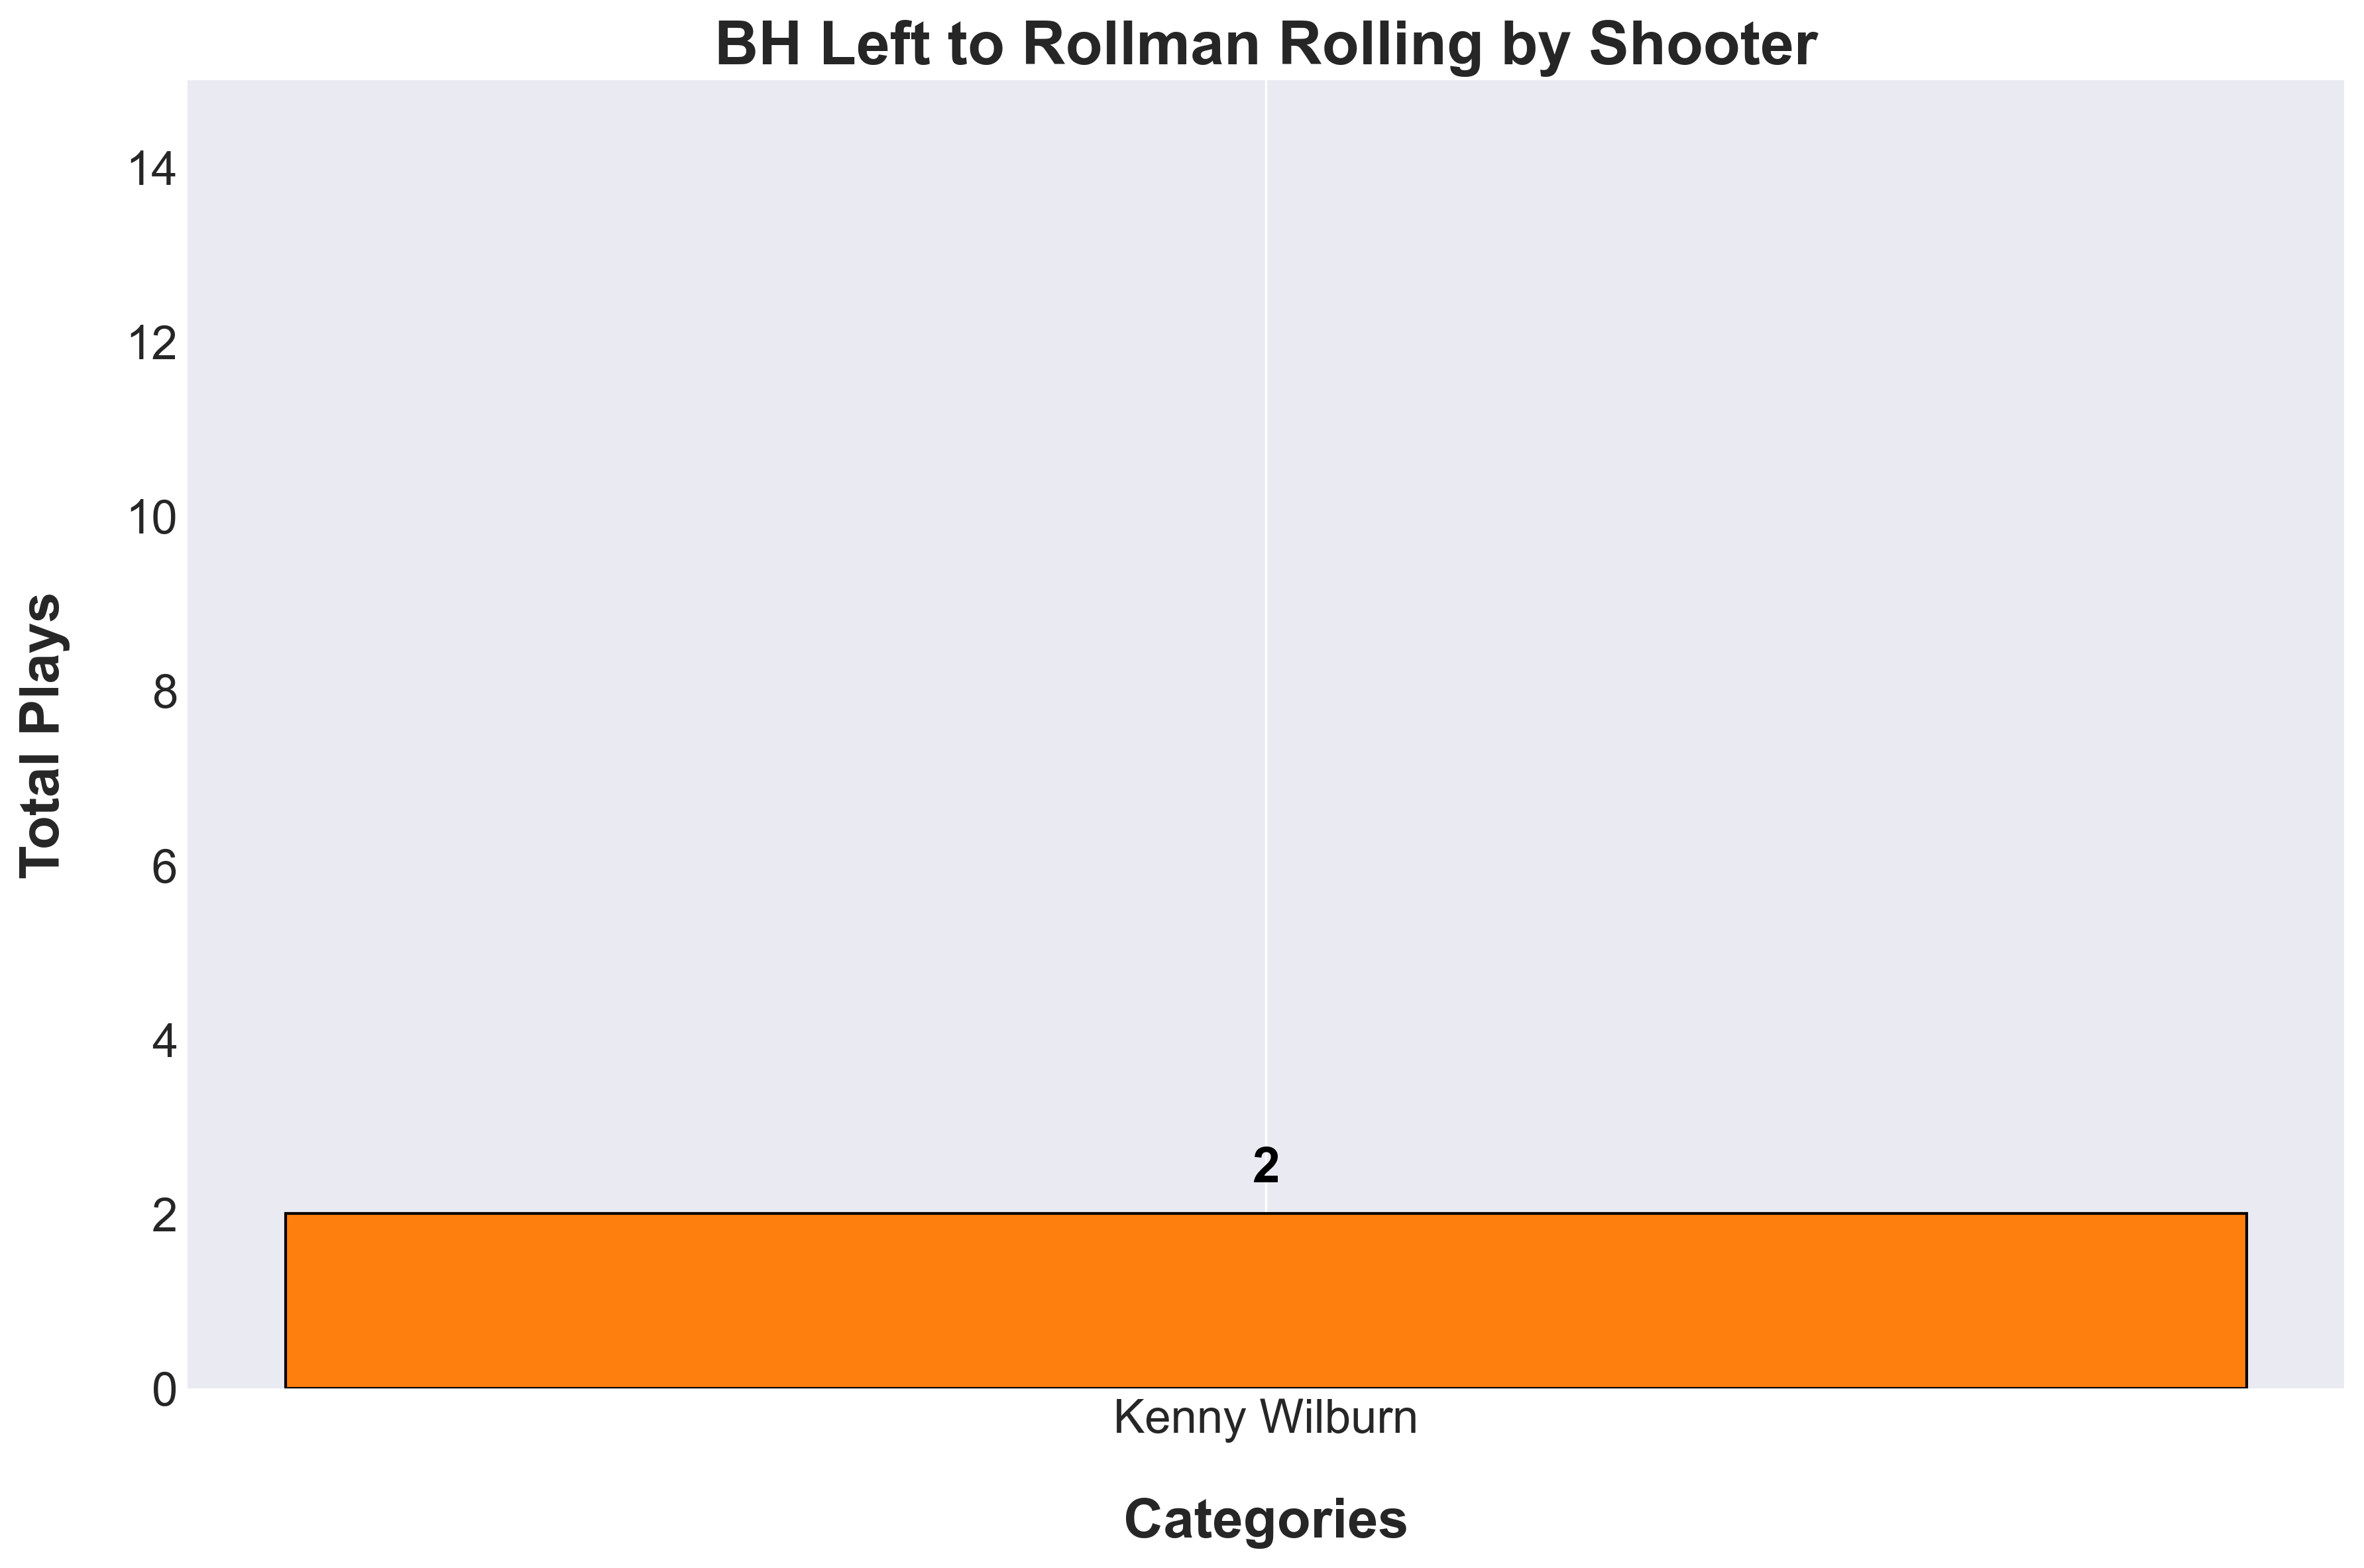
\includegraphics[width=\textwidth, height=.14\textheight]{images/PNR_PassLeftRollsPlayer_Freq.png} % Adjust the width of the image to fit
    \end{minipage}
\end{table}

\vspace{-1em} % Add vertical space before the line (optional)
%\hrule height 1pt width 1\textwidth % Adjust height and width
\vspace{-1em} % Add vertical space after the line (optional)

% BH Left -> Rollman Slips Secondary Player Stats
\begin{table}[H]
    \raisebox{3em}{ % Adjust this value to shift the tables vertically
    \begin{minipage}[t]{0.6\textwidth} % Left side (table) takes 85% of the width
        \flushleft
        \centering % Centering the title and the table
        \text{BH Left - Rollman Slips Player Statistics} % Title above the table in bold
        \vskip .25em % Adds vertical space between title and table
        \scalebox{.55}{ % Scale the entire table down by half
            \renewcommand{\arraystretch}{1.4} % Adjust the number to increase or decrease row spacing
            \begin{tabular}{
            >{\centering\arraybackslash}p{3cm} 
            >{\centering\arraybackslash}p{.75cm} 
            >{\centering\arraybackslash}p{.75cm} 
            >{\centering\arraybackslash}p{.75cm} 
            >{\centering\arraybackslash}p{.75cm}
            >{\centering\arraybackslash}p{.75cm} 
            >{\centering\arraybackslash}p{.75cm} 
            >{\centering\arraybackslash}p{.75cm} 
            >{\centering\arraybackslash}p{.75cm}
            >{\centering\arraybackslash}p{.75cm} 
            >{\centering\arraybackslash}p{.75cm}
            >{\centering\arraybackslash}p{.75cm} 
            >{\centering\arraybackslash}p{.75cm}}% Adjust column widths
            \toprule
            {\scriptsize \textbf{Player}} &
            {\scriptsize \textbf{Plays}} &
            {\scriptsize \textbf{3PA}} &
            {\scriptsize \textbf{3PM}} &
            {\scriptsize \textbf{3P\%}} & 
            {\scriptsize \textbf{2PA}} & 
            {\scriptsize \textbf{2PM}} & 
            {\scriptsize \textbf{2P\%}} & 
            {\scriptsize \textbf{MiA}} & 
            {\scriptsize \textbf{MiM}} &
            {\scriptsize \textbf{Mi\%}} &
            {\scriptsize \textbf{TO}} &
            {\scriptsize \textbf{Foul}} \\
            \midrule
            
                
            
                
            
                
            
                
            
                
            
                
            
                
            
                
            
                
            
                
            
                
            
                
            
                
            
                
            
                
            
                
            
                
                    
                
            
                
            
                
            
                
            
                
            
                
            
                
            
                
            
                
            
                
            
                
            
                
            
                
            
                
            
                
            
                
            
                
            
                
            
                
            
                
            
                
            
                
            

            \bottomrule
        \end{tabular}
        } % End of \scalebox
    \end{minipage}
    } % End of raisebox, closing the adjustment
    \hfill % This adds some flexible space between the table and the image
    \begin{minipage}[c]{0.35\textwidth} % Right side (image) takes 10% of the width
        \flushright
        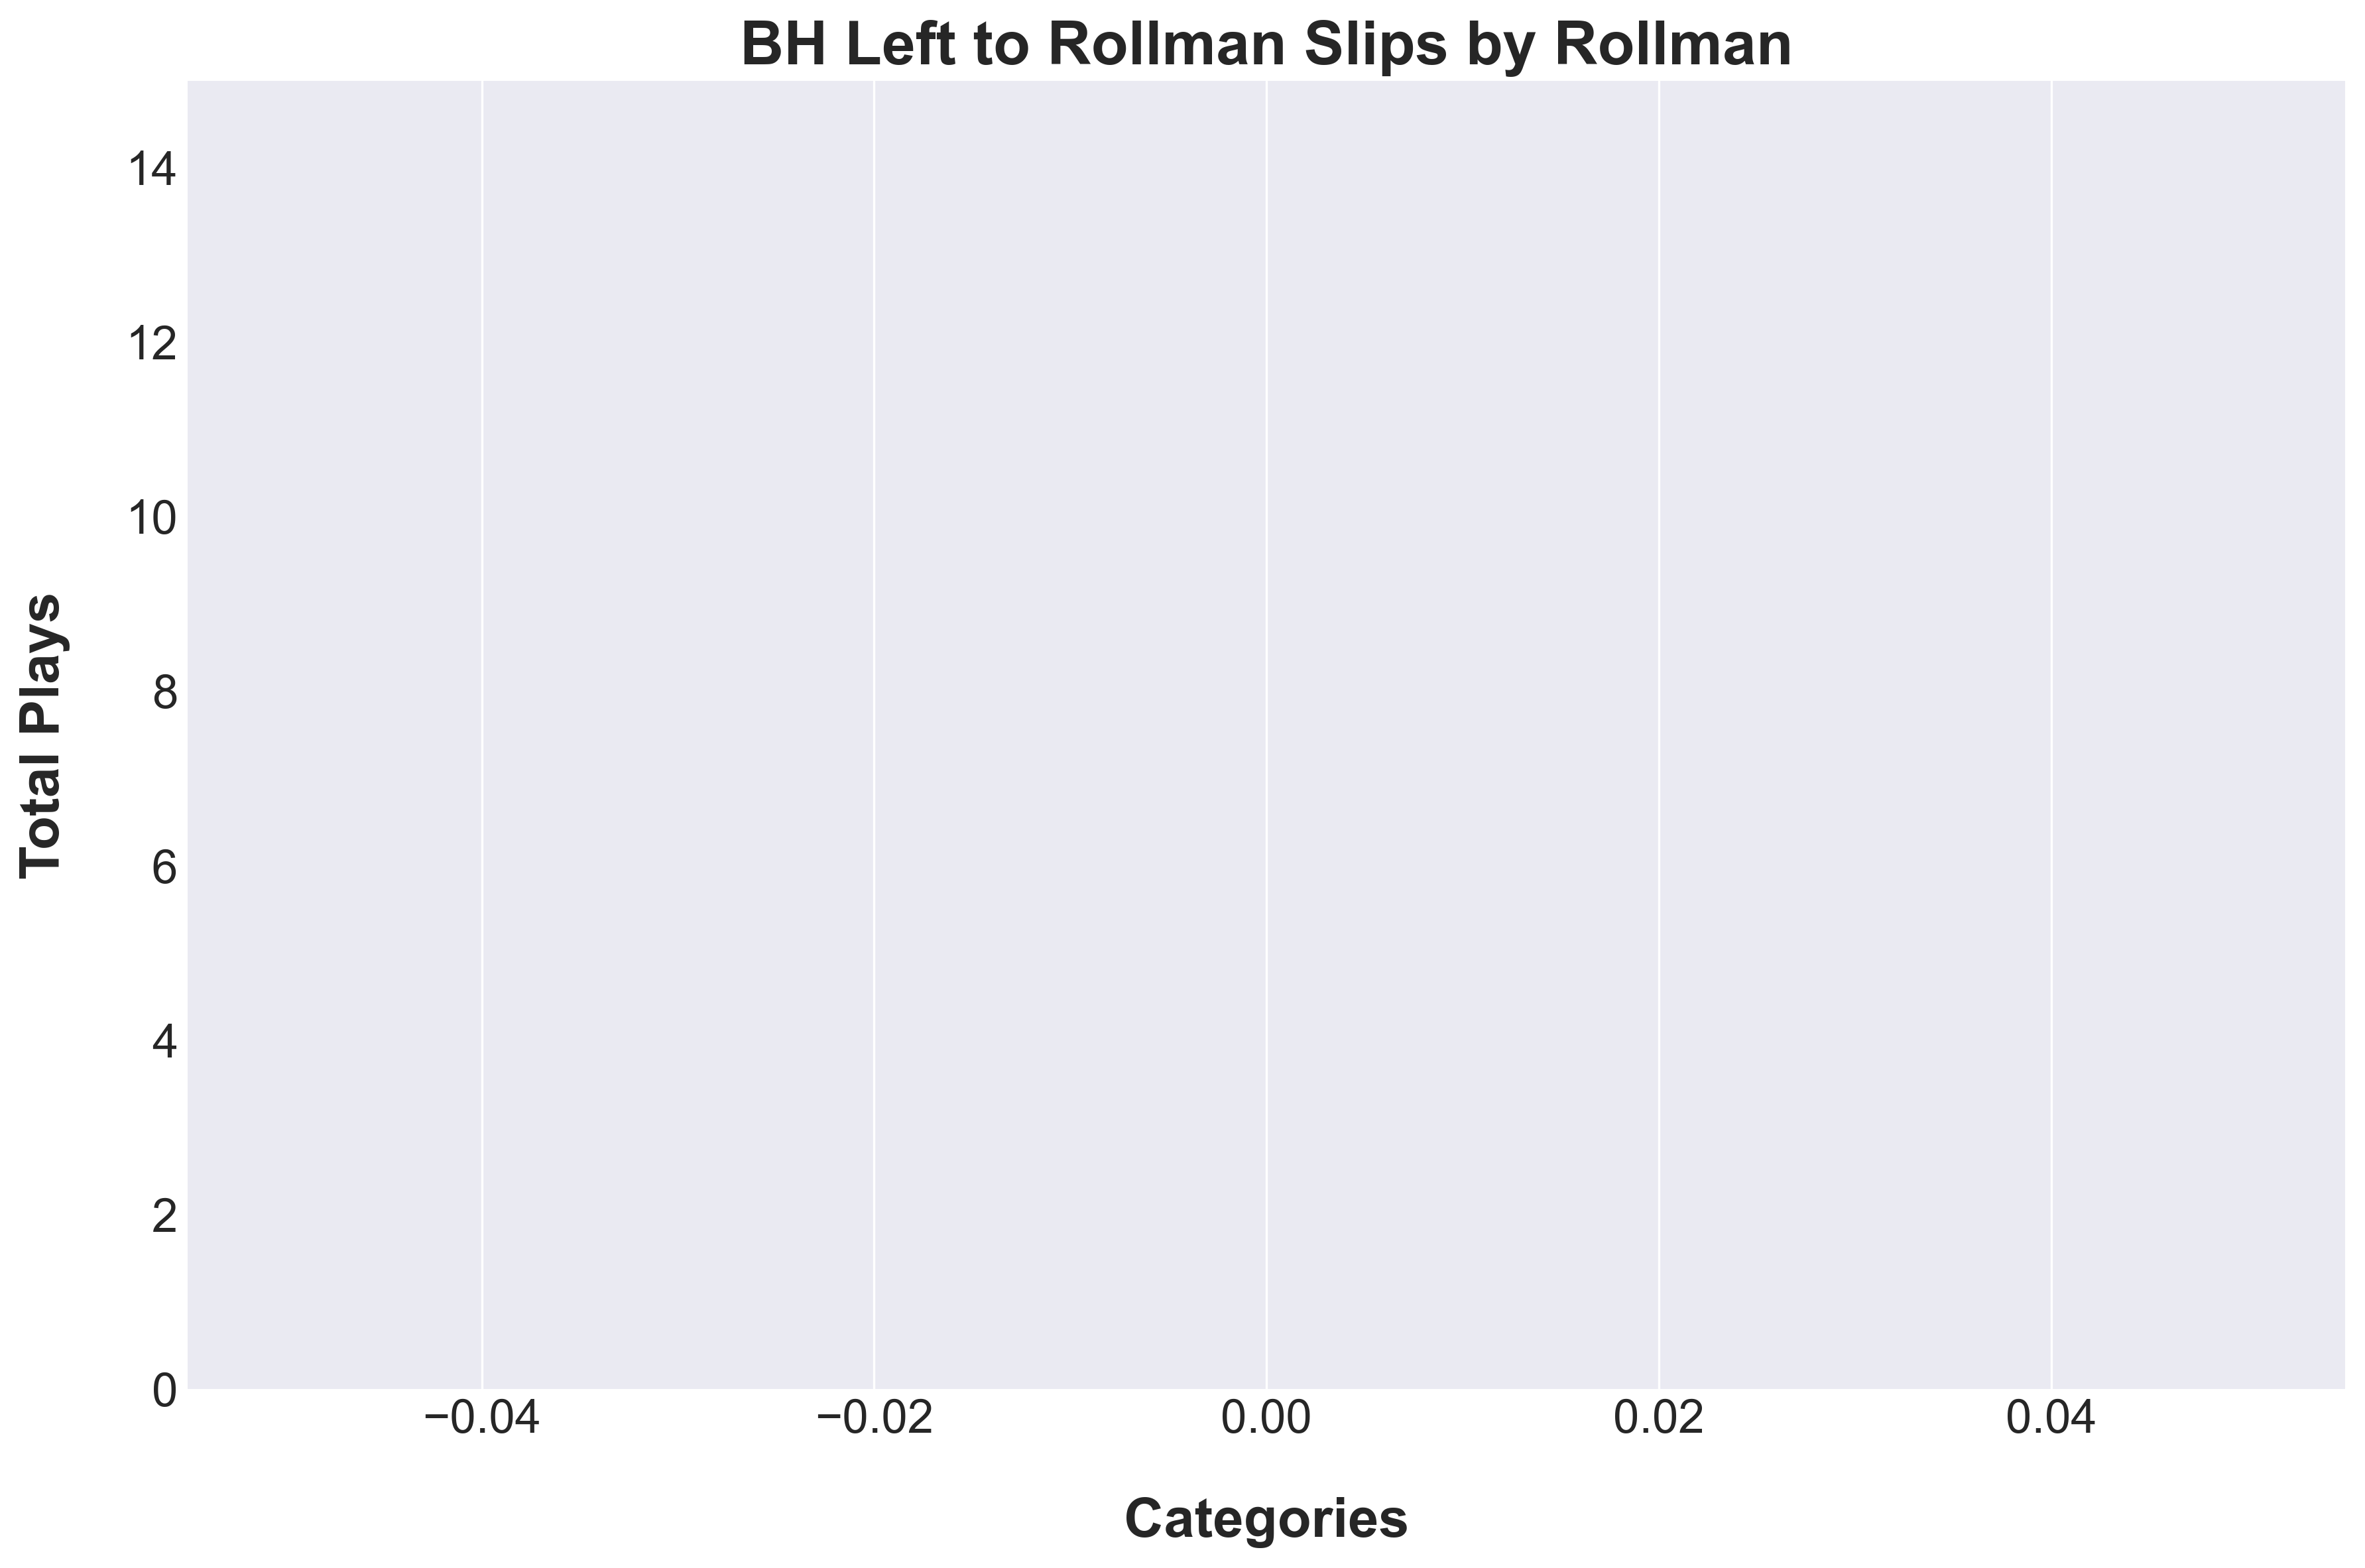
\includegraphics[width=\textwidth, height=.14\textheight]{images/PNR_PassLeftSlipsPlayer_Freq.png} % Adjust the width of the image to fit
    \end{minipage}
\end{table}

\vspace{-1em} % Add vertical space before the line (optional)
%\hrule height 1pt width 1\textwidth % Adjust height and width
\vspace{-1em} % Add vertical space after the line (optional)

% BH Left -> Rollman Pops Secondary Player Stats
\begin{table}[H]
    \raisebox{3em}{ % Adjust this value to shift the tables vertically
    \begin{minipage}[t]{0.6\textwidth} % Left side (table) takes 85% of the width
        \flushleft
        \centering % Centering the title and the table
        \text{BH Left - Rollman Pops Player Statistics} % Title above the table in bold
        \vskip .25em % Adds vertical space between title and table
        \scalebox{.55}{ % Scale the entire table down by half
            \renewcommand{\arraystretch}{1.4} % Adjust the number to increase or decrease row spacing
            \begin{tabular}{
            >{\centering\arraybackslash}p{3cm} 
            >{\centering\arraybackslash}p{.75cm} 
            >{\centering\arraybackslash}p{.75cm} 
            >{\centering\arraybackslash}p{.75cm} 
            >{\centering\arraybackslash}p{.75cm}
            >{\centering\arraybackslash}p{.75cm} 
            >{\centering\arraybackslash}p{.75cm} 
            >{\centering\arraybackslash}p{.75cm} 
            >{\centering\arraybackslash}p{.75cm}
            >{\centering\arraybackslash}p{.75cm} 
            >{\centering\arraybackslash}p{.75cm}
            >{\centering\arraybackslash}p{.75cm} 
            >{\centering\arraybackslash}p{.75cm}}% Adjust column widths
            \toprule
            {\scriptsize \textbf{Player}} &
            {\scriptsize \textbf{Plays}} &
            {\scriptsize \textbf{3PA}} &
            {\scriptsize \textbf{3PM}} &
            {\scriptsize \textbf{3P\%}} & 
            {\scriptsize \textbf{2PA}} & 
            {\scriptsize \textbf{2PM}} & 
            {\scriptsize \textbf{2P\%}} & 
            {\scriptsize \textbf{MiA}} & 
            {\scriptsize \textbf{MiM}} &
            {\scriptsize \textbf{Mi\%}} &
            {\scriptsize \textbf{TO}} &
            {\scriptsize \textbf{Foul}} \\
            \midrule
            
                
            
                
            
                
            
                
            
                
            
                
            
                
            
                
            
                
            
                
            
                
            
                
            
                
            
                
            
                
            
                
            
                
            
                
                    
                        Josiah Turner & 
                        1 & 
                        0 & 
                        0 & 
                        - & 
                        1 & 
                        0 & 
                        0.0 & 
                        0 & 
                        0 & 
                        - & 
                        0 & 
                        0 \\
                    
                
            
                
            
                
            
                
            
                
            
                
            
                
            
                
            
                
            
                
            
                
            
                
            
                
            
                
            
                
            
                
            
                
            
                
            
                
            
                
            
                
            


            \bottomrule
        \end{tabular}
        } % End of \scalebox
    \end{minipage}
    } % End of raisebox, closing the adjustment
    \hfill % This adds some flexible space between the table and the image
    \begin{minipage}[c]{0.35\textwidth} % Right side (image) takes 10% of the width
        \flushright
        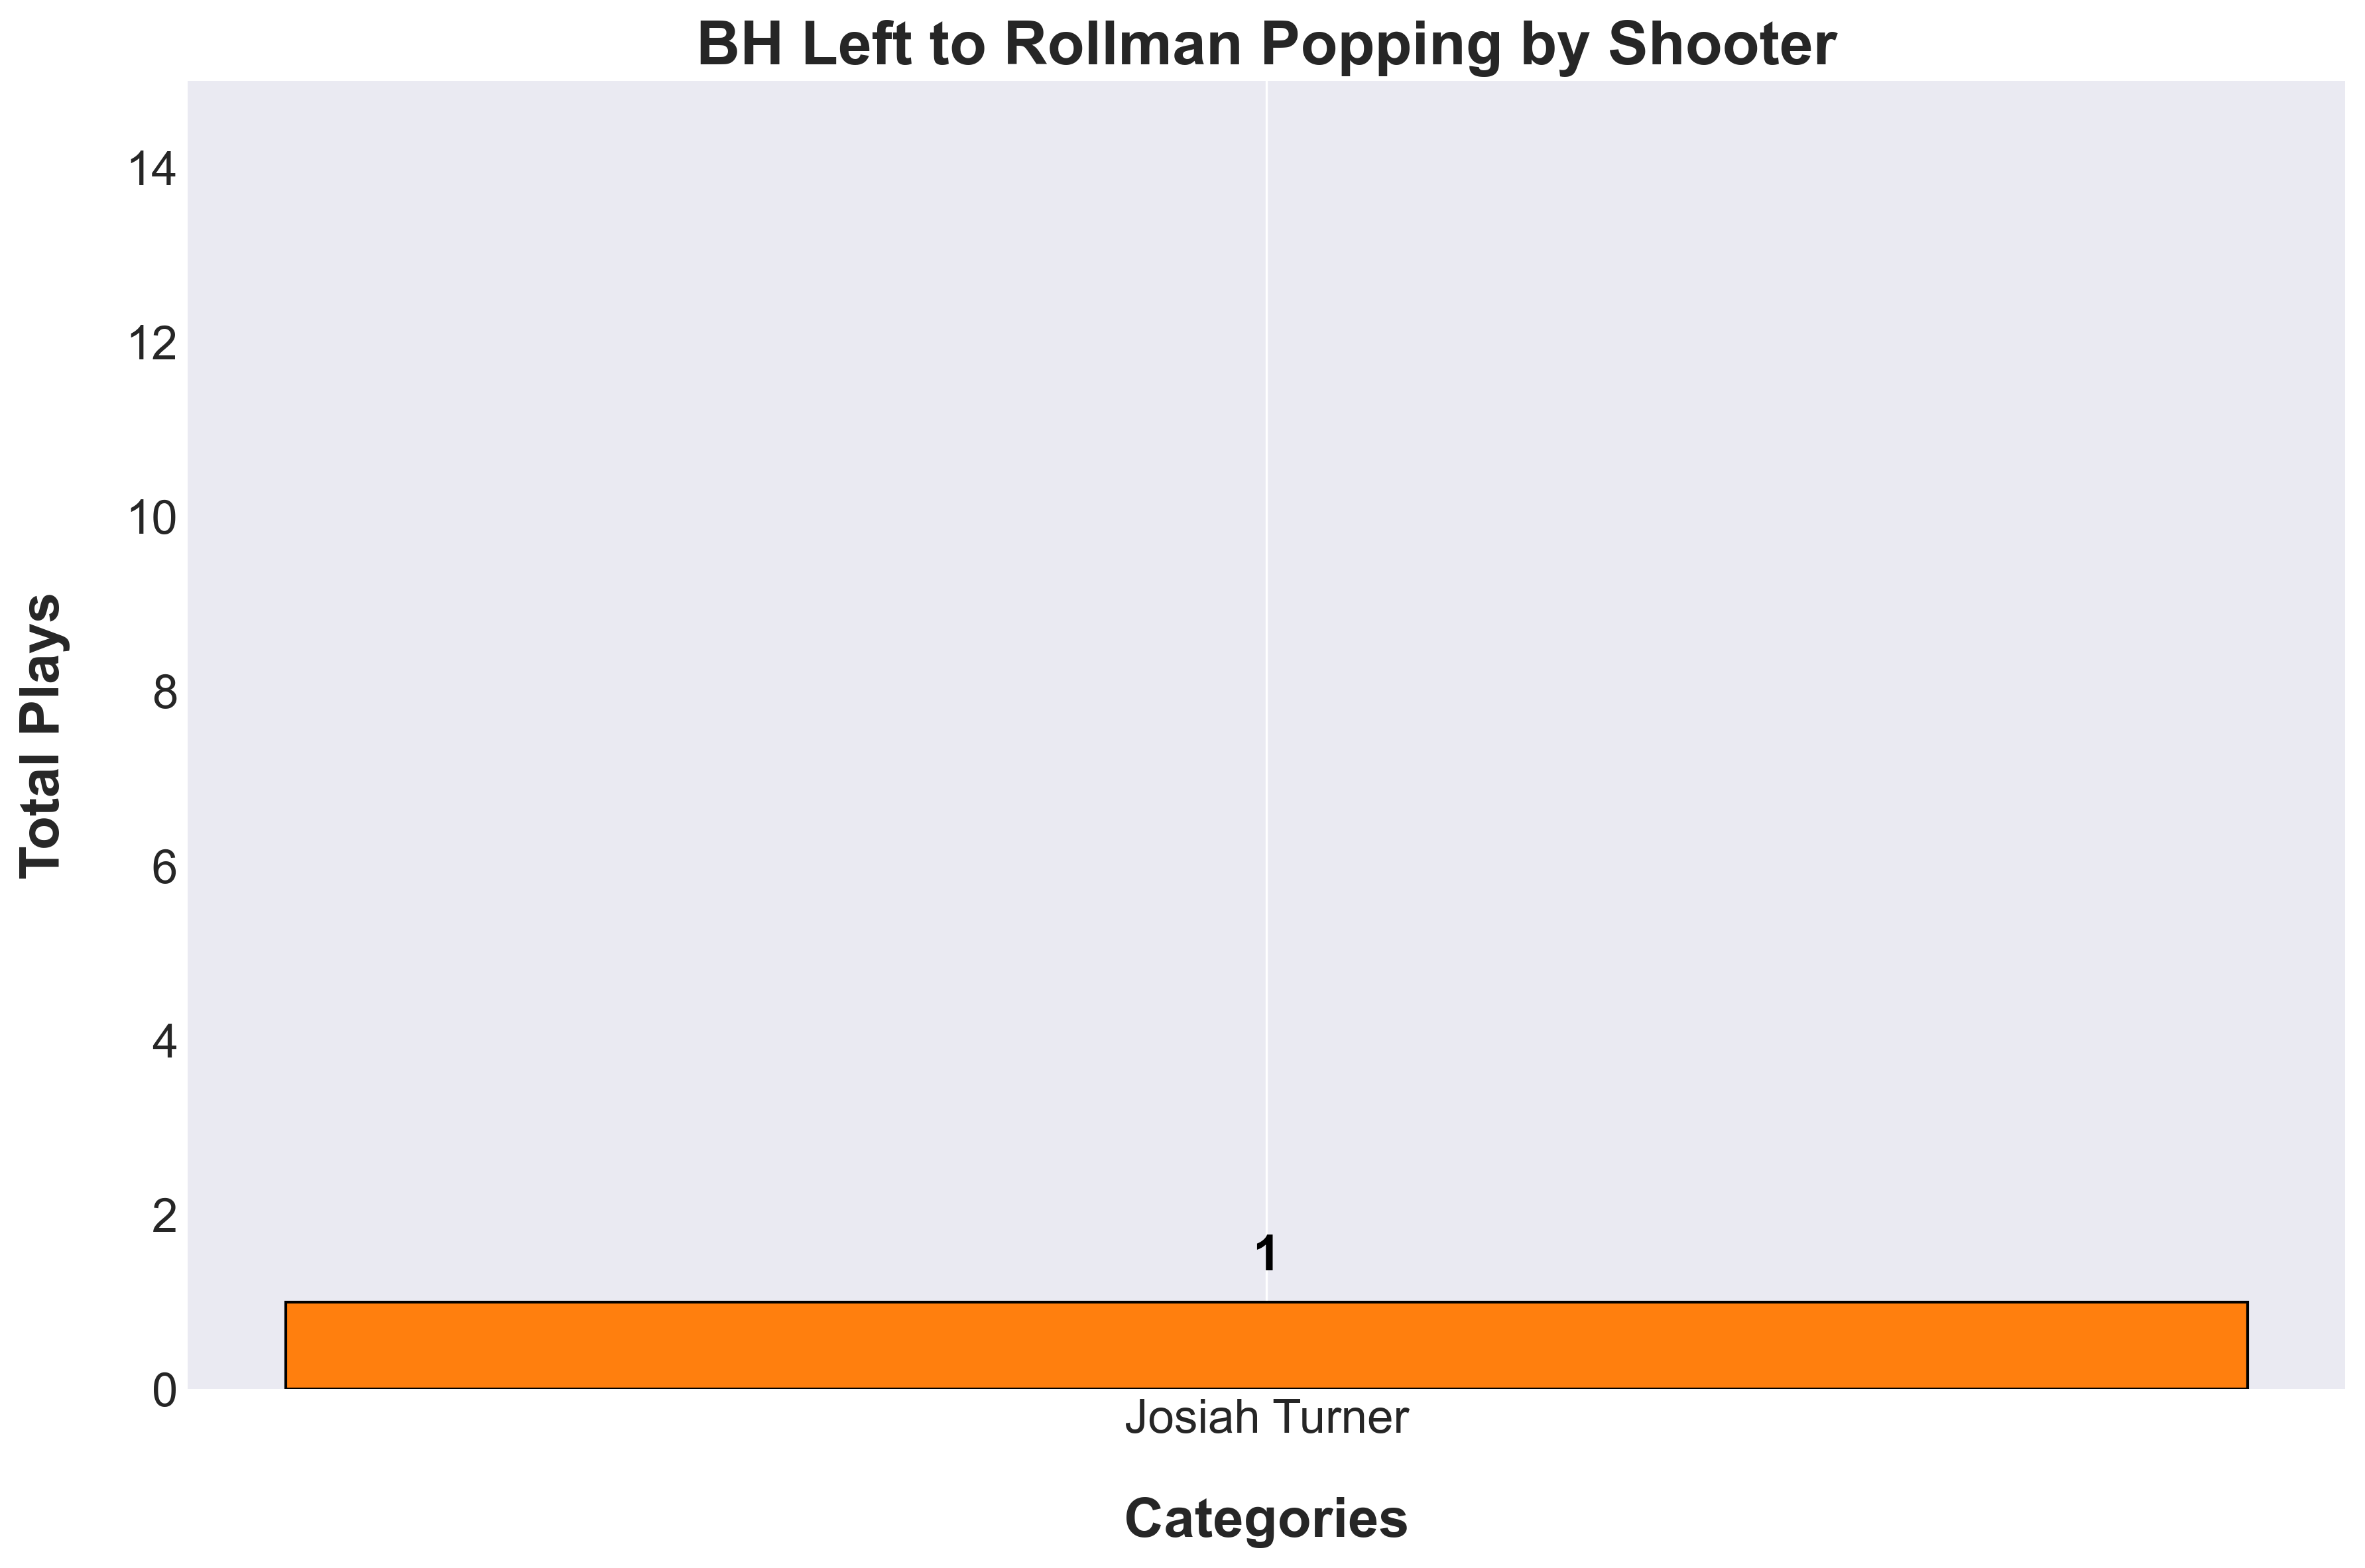
\includegraphics[width=\textwidth, height=.14\textheight]{images/PNR_PassLeftPopsPlayer_Freq.png} % Adjust the width of the image to fit
    \end{minipage}
\end{table}

\vspace{-1em} % Add vertical space before the line (optional)
\hrule height 1pt width 1\textwidth % Adjust height and width
\vspace{1em} % Add vertical space after the line (optional)

\subsubsection{BH Right PNR Passer Statistics}

% BH Right -> Cuts Secondary Player Stats
\begin{table}[H]
    \raisebox{3em}{ % Adjust this value to shift the tables vertically
    \begin{minipage}[t]{0.6\textwidth} % Left side (table) takes 85% of the width
        \flushleft
        \centering % Centering the title and the table
        \text{BH Right - Cuts Player Statistics} % Title above the table in bold
        \vskip .25em % Adds vertical space between title and table
        \scalebox{.6}{ % Scale the entire table down by half
            \renewcommand{\arraystretch}{1.4} % Adjust the number to increase or decrease row spacing
            \begin{tabular}{
            >{\centering\arraybackslash}p{3cm} 
            >{\centering\arraybackslash}p{.75cm} 
            >{\centering\arraybackslash}p{.75cm} 
            >{\centering\arraybackslash}p{.75cm} 
            >{\centering\arraybackslash}p{.75cm}
            >{\centering\arraybackslash}p{.75cm} 
            >{\centering\arraybackslash}p{.75cm}
            >{\centering\arraybackslash}p{.75cm}
            >{\centering\arraybackslash}p{.75cm} 
            >{\centering\arraybackslash}p{.75cm}}% Adjust column widths
            \toprule
            {\scriptsize \textbf{Player}} &
            {\scriptsize \textbf{Plays}} &
            {\scriptsize \textbf{2PA}} & 
            {\scriptsize \textbf{2PM}} & 
            {\scriptsize \textbf{2P\%}} & 
            {\scriptsize \textbf{MiA}} & 
            {\scriptsize \textbf{MiM}} &
            {\scriptsize \textbf{Mi\%}} &
            {\scriptsize \textbf{TO}} &
            {\scriptsize \textbf{Foul}} \\
            \midrule
            
                
            
                
            
                
            
                
            
                
            
                
            
                
            
                
            
                
            
                
            
                
            
                
            
                
            
                
            
                
            
                
            
                
            
                
            
                
                    
                        Nolan Smih & 
                        1 & 
                        1 & 
                        1 & 
                        100.0 & 
                        0 & 
                        0 & 
                        - & 
                        0 & 
                        0 \\
                    
                
            
                
            
                
            
                
            
                
            
                
            
                
            
                
            
                
            
                
            
                
            
                
            
                
            
                
            
                
            
                
            
                
            
                
            
                
            
                
            

            \bottomrule
        \end{tabular}
        } % End of \scalebox
    \end{minipage}
    } % End of raisebox, closing the adjustment
    \hfill % This adds some flexible space between the table and the image
    \begin{minipage}[c]{0.35\textwidth} % Right side (image) takes 10% of the width
        \flushright
        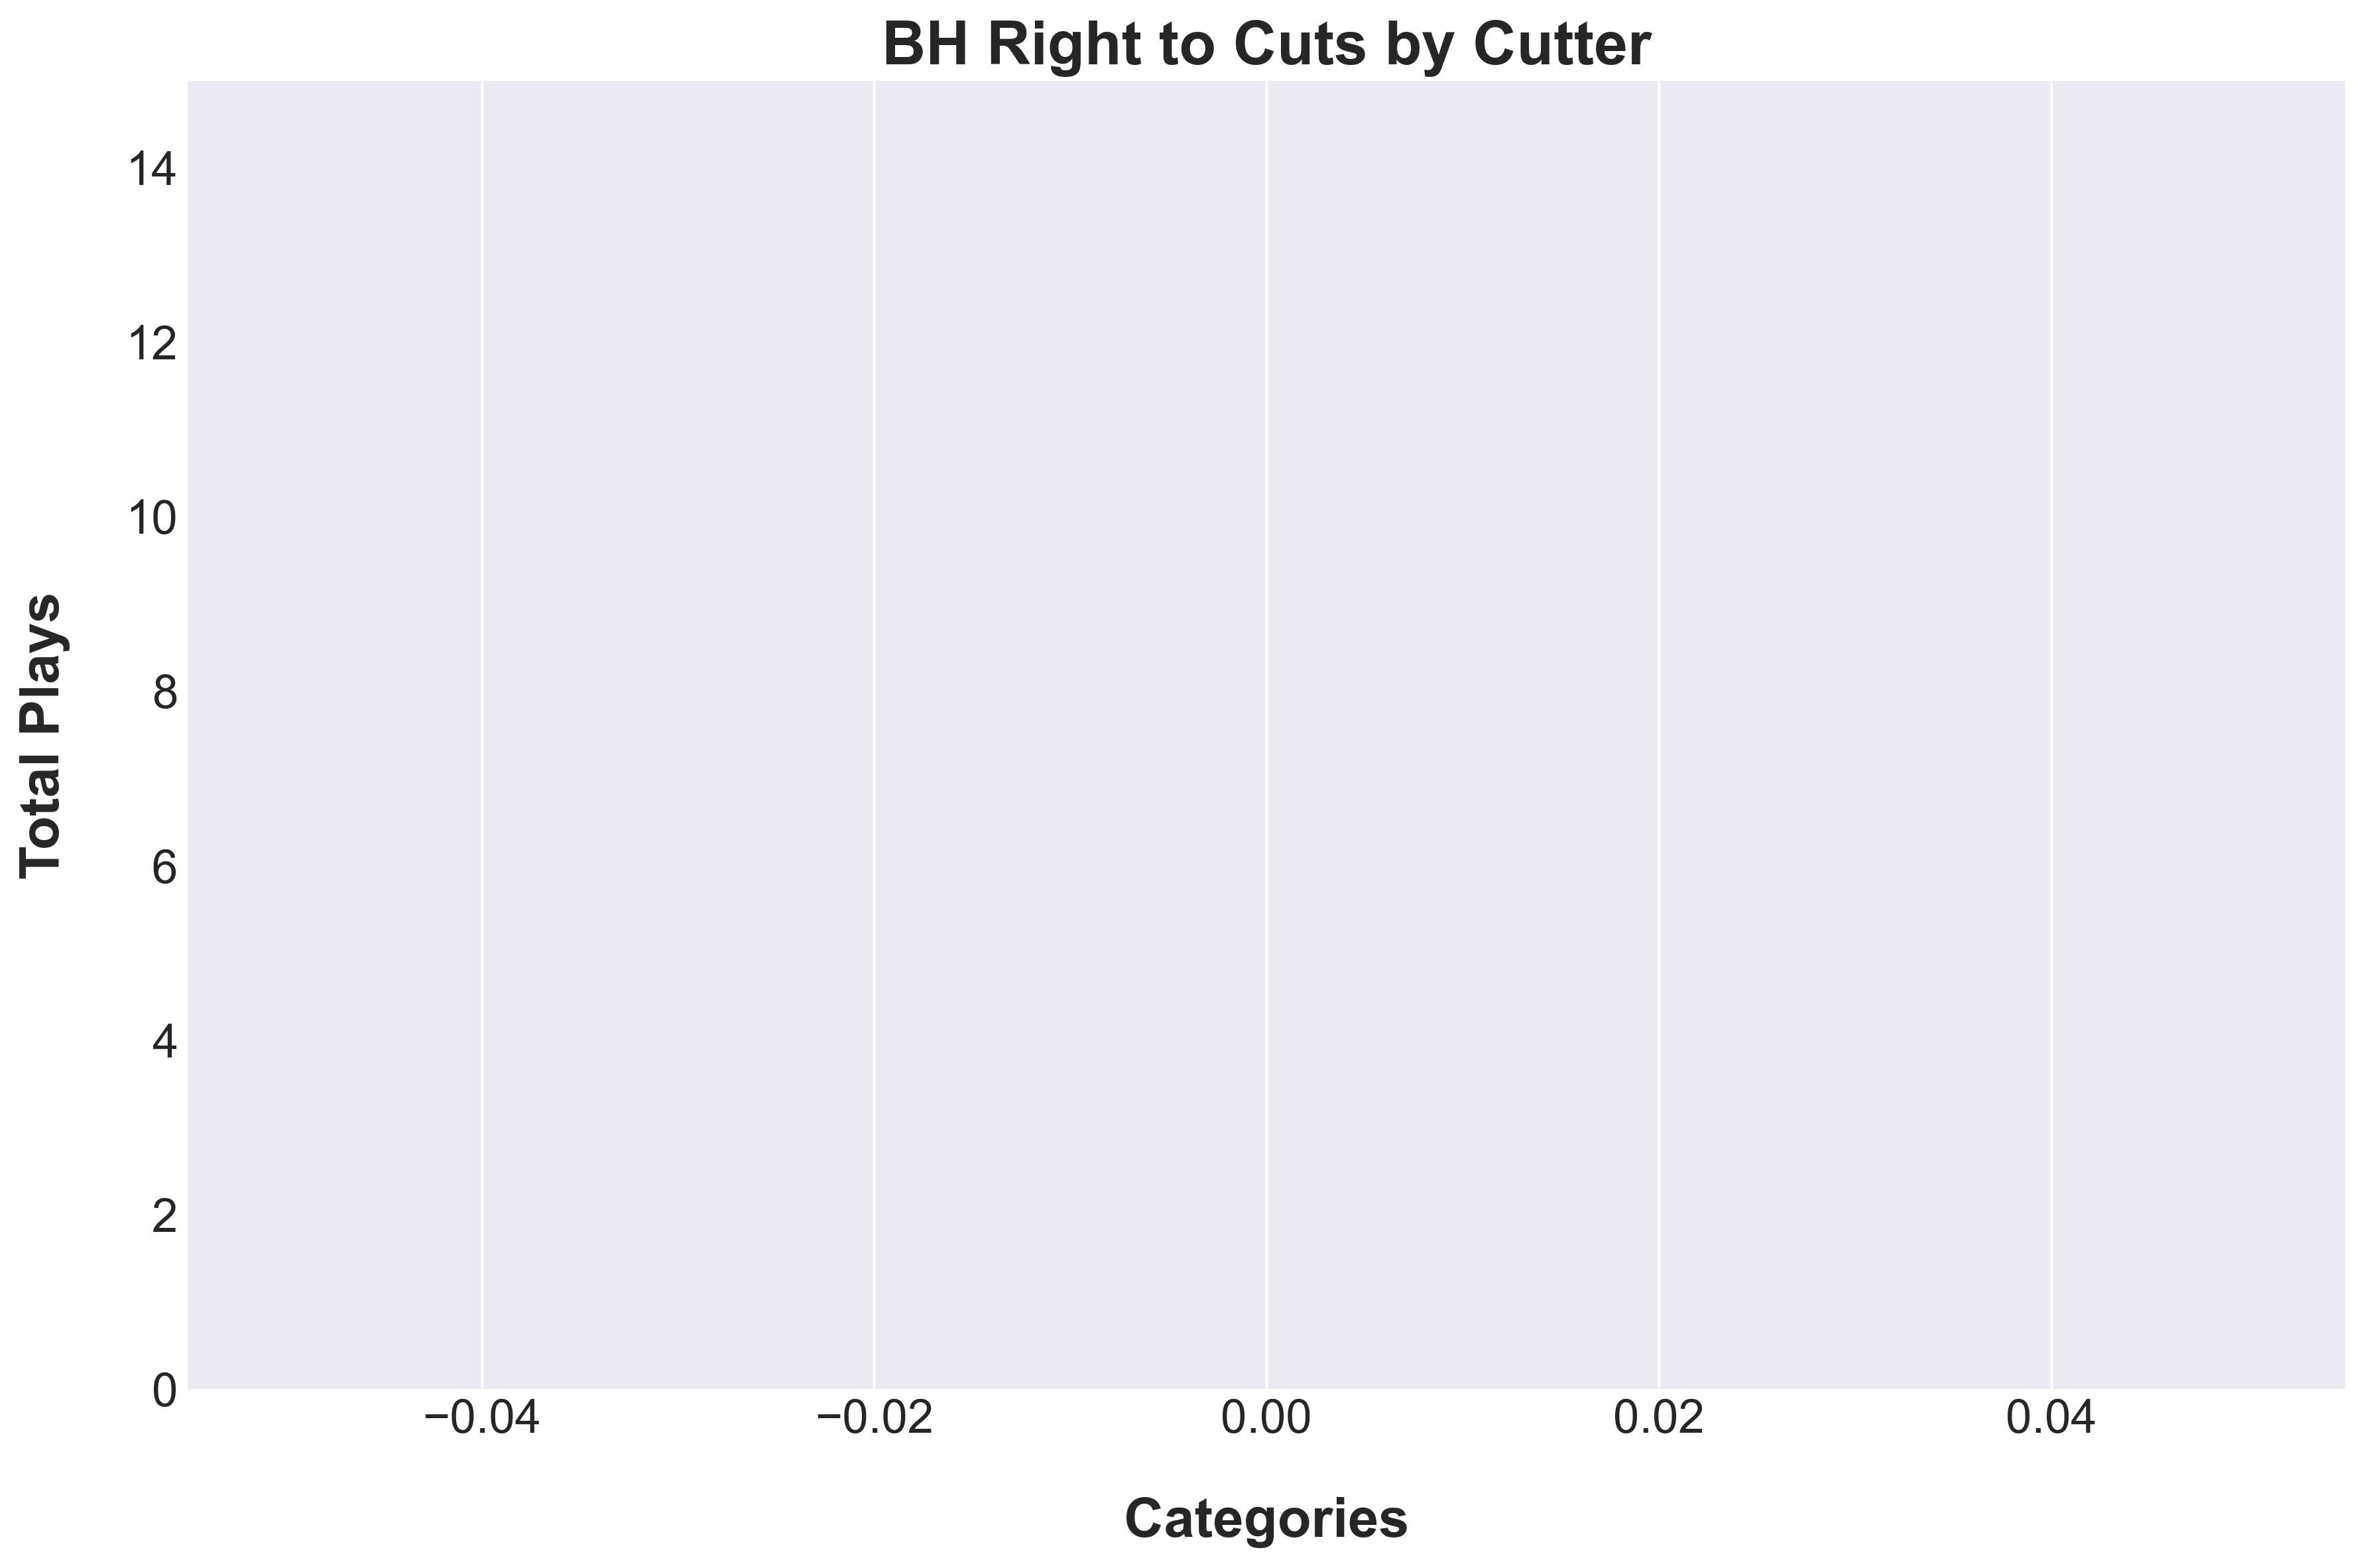
\includegraphics[width=\textwidth, height=.14\textheight]{images/PNR_PassRightCutsPlayer_Freq.png} % Adjust the width of the image to fit
    \end{minipage}
\end{table}

\vspace{-1em} % Add vertical space before the line (optional)
%\hrule height 1pt width 1\textwidth % Adjust height and width
\vspace{-1em} % Add vertical space after the line (optional)

% BH Right -> Spot Up Drives Secondary Player Stats
\begin{table}[H]
    \raisebox{3em}{ % Adjust this value to shift the tables vertically
    \begin{minipage}[t]{0.6\textwidth} % Left side (table) takes 85% of the width
        \flushleft
        \centering % Centering the title and the table
        \text{BH Right - Spot Up Drives Player Statistics} % Title above the table in bold
        \vskip .25em % Adds vertical space between title and table
        \scalebox{.55}{ % Scale the entire table down by half
            \renewcommand{\arraystretch}{1.4} % Adjust the number to increase or decrease row spacing
            \begin{tabular}{
            >{\centering\arraybackslash}p{3cm} 
            >{\centering\arraybackslash}p{.75cm} 
            >{\centering\arraybackslash}p{.75cm} 
            >{\centering\arraybackslash}p{.75cm} 
            >{\centering\arraybackslash}p{.75cm}
            >{\centering\arraybackslash}p{.75cm} 
            >{\centering\arraybackslash}p{.75cm} 
            >{\centering\arraybackslash}p{.75cm} 
            >{\centering\arraybackslash}p{.75cm}
            >{\centering\arraybackslash}p{.75cm} 
            >{\centering\arraybackslash}p{.75cm}
            >{\centering\arraybackslash}p{.75cm} 
            >{\centering\arraybackslash}p{.75cm}}% Adjust column widths
            \toprule
            {\scriptsize \textbf{Player}} &
            {\scriptsize \textbf{Plays}} &
            {\scriptsize \textbf{3PA}} &
            {\scriptsize \textbf{3PM}} &
            {\scriptsize \textbf{3P\%}} & 
            {\scriptsize \textbf{2PA}} & 
            {\scriptsize \textbf{2PM}} & 
            {\scriptsize \textbf{2P\%}} & 
            {\scriptsize \textbf{MiA}} & 
            {\scriptsize \textbf{MiM}} &
            {\scriptsize \textbf{Mi\%}} &
            {\scriptsize \textbf{TO}} &
            {\scriptsize \textbf{Foul}} \\
            \midrule
            
                
            
                
            
                
            
                
            
                
            
                
            
                
            
                
            
                
            
                
            
                
            
                
            
                
            
                
            
                
            
                
            
                
            
                
            
                
            
                
                    
                        Brock Bowen & 
                        1 & 
                        0 & 
                        0 & 
                        - & 
                        0 & 
                        0 & 
                        - & 
                        0 & 
                        0 & 
                        - & 
                        1 & 
                        0 \\
                    
                        Chase Dickens & 
                        1 & 
                        1 & 
                        0 & 
                        0.0 & 
                        0 & 
                        0 & 
                        - & 
                        0 & 
                        0 & 
                        - & 
                        0 & 
                        0 \\
                    
                        Mark Osime & 
                        1 & 
                        0 & 
                        0 & 
                        - & 
                        0 & 
                        0 & 
                        - & 
                        0 & 
                        0 & 
                        - & 
                        0 & 
                        1 \\
                    
                
            
                
            
                
            
                
            
                
            
                
            
                
            
                
            
                
            
                
            
                
            
                
            
                
            
                
            
                
            
                
            
                
            
                
            
                
            

            \bottomrule
        \end{tabular}
        } % End of \scalebox
    \end{minipage}
    } % End of raisebox, closing the adjustment
    \hfill % This adds some flexible space between the table and the image
    \begin{minipage}[c]{0.35\textwidth} % Right side (image) takes 10% of the width
        \flushright
        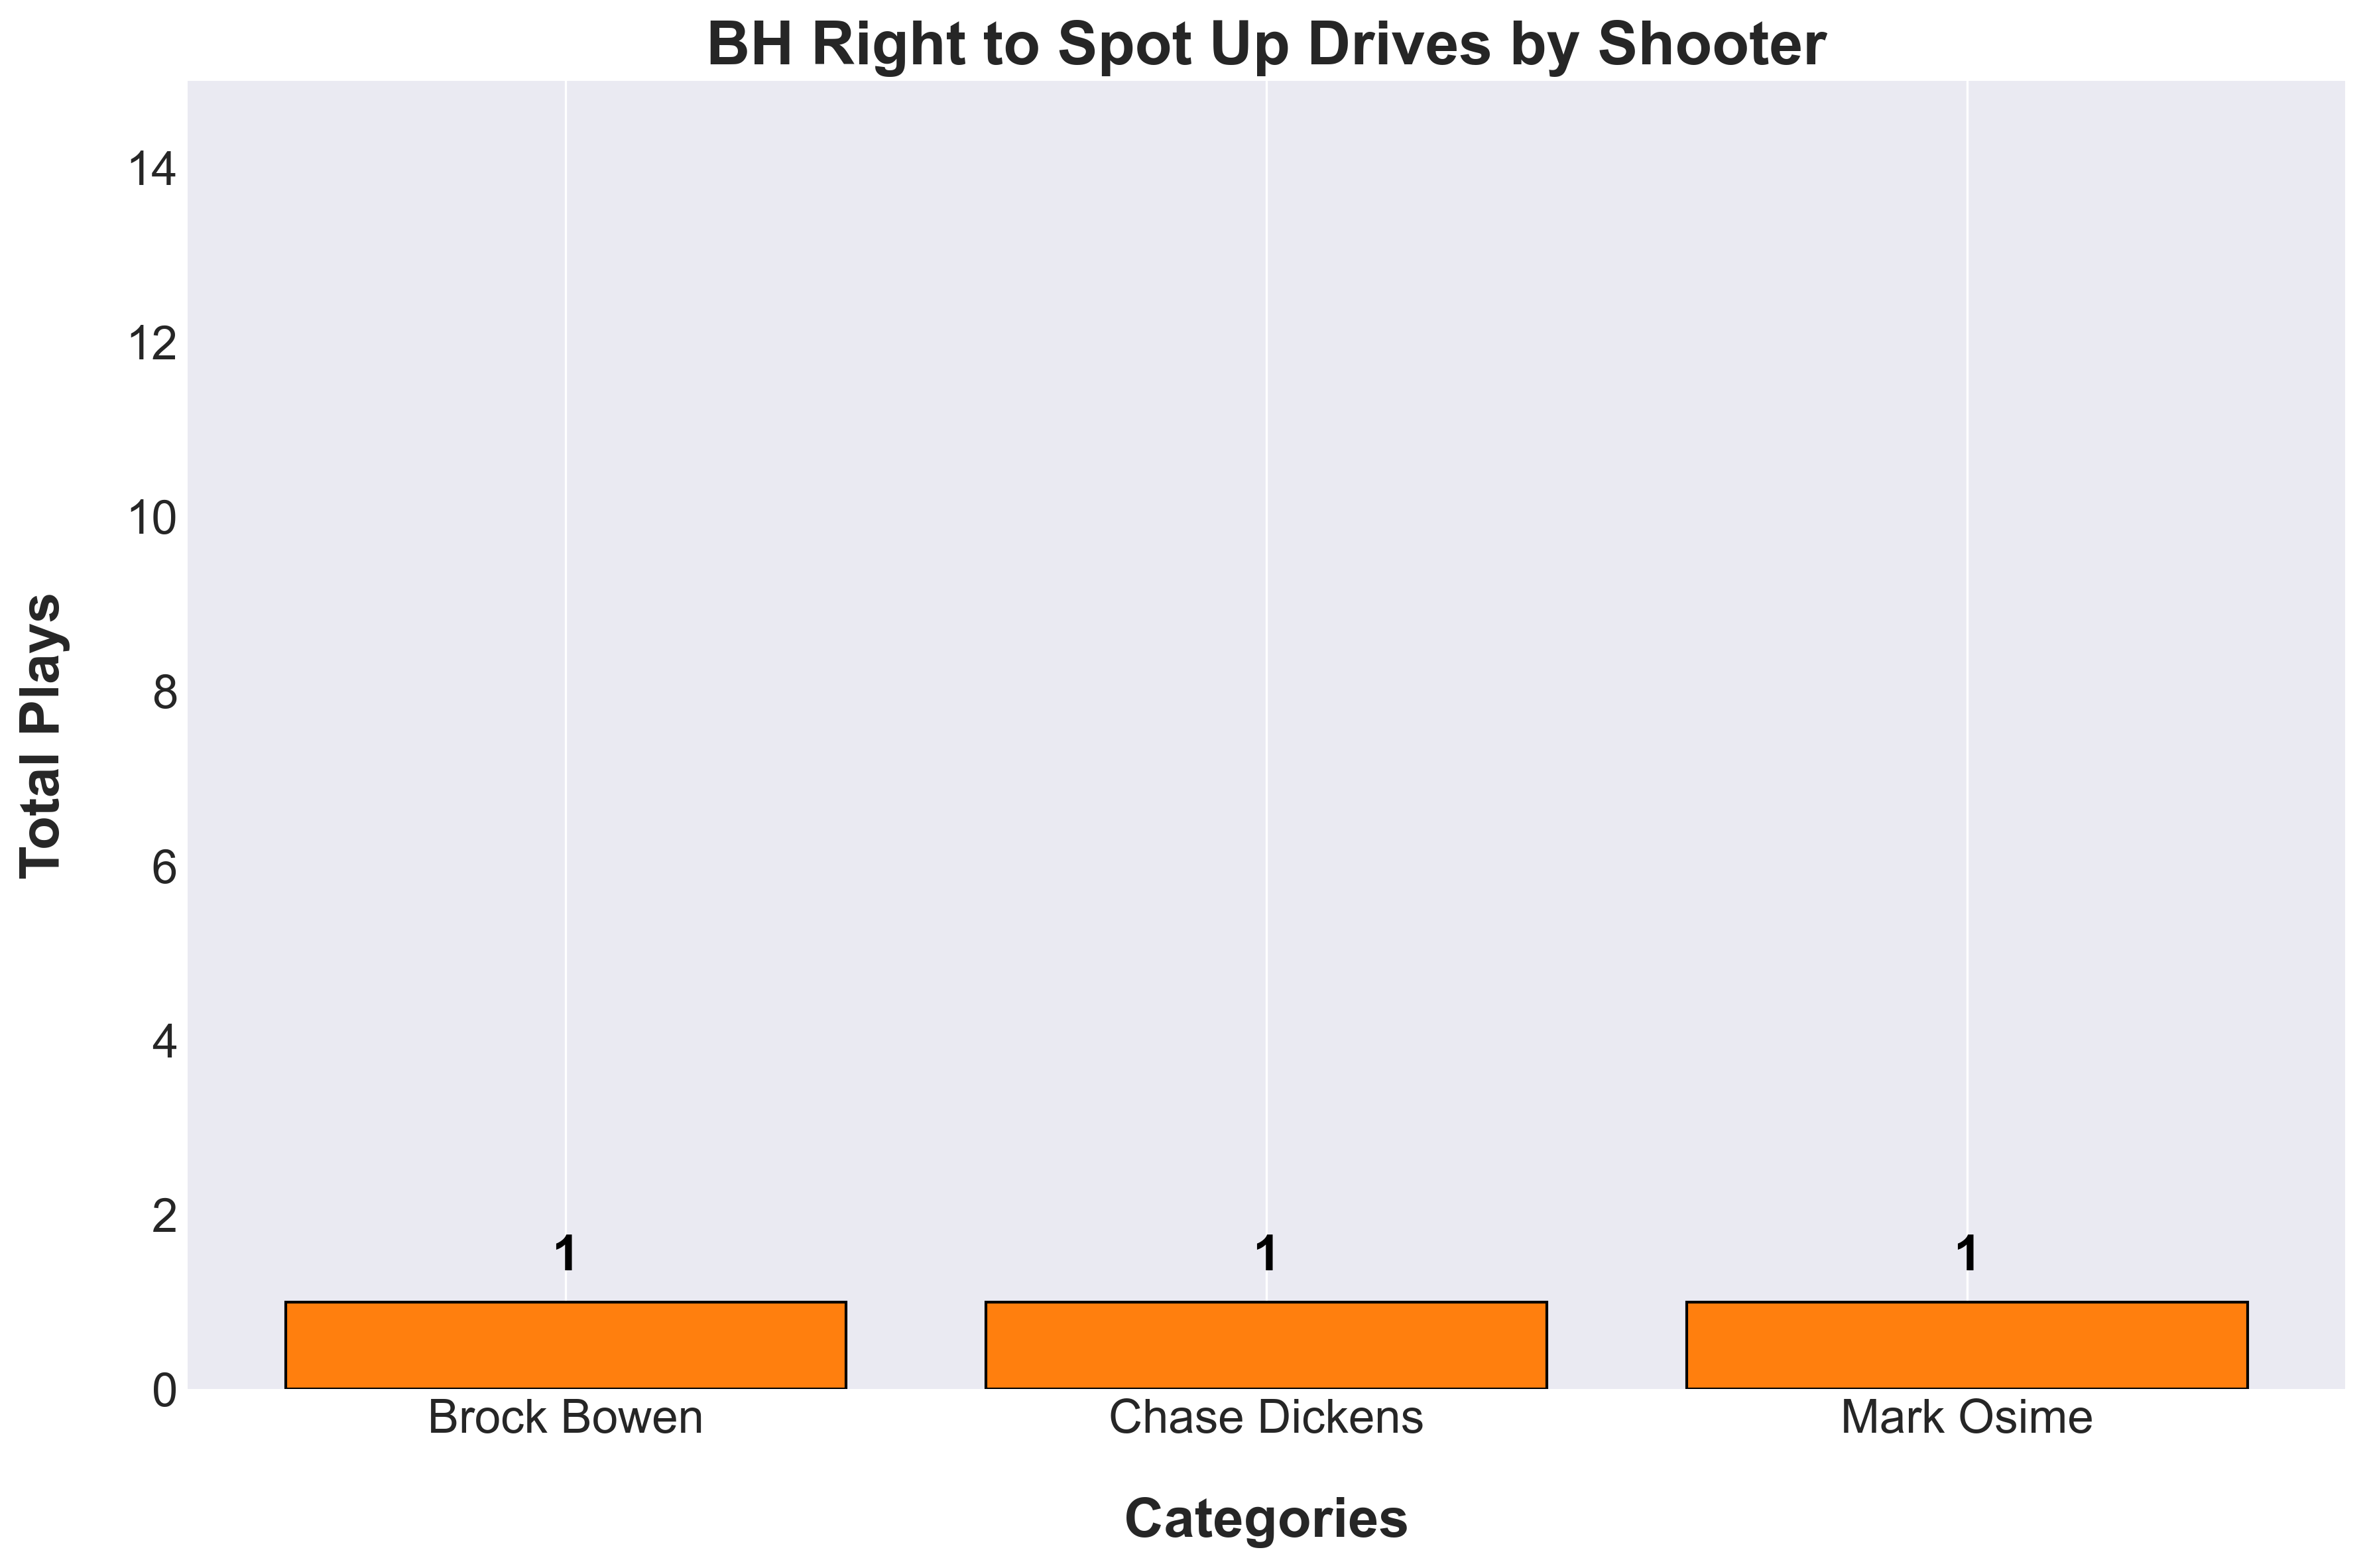
\includegraphics[width=\textwidth, height=.14\textheight]{images/PNR_PassRightDrivesPlayer_Freq.png} % Adjust the width of the image to fit
    \end{minipage}
\end{table}

\vspace{-1em} % Add vertical space before the line (optional)
%\hrule height 1pt width 1\textwidth % Adjust height and width
\vspace{-1em} % Add vertical space after the line (optional)

% BH Right -> Spot Up Shots Secondary Player Stats
\begin{table}[H]
    \raisebox{3em}{ % Adjust this value to shift the tables vertically
    \begin{minipage}[t]{0.6\textwidth} % Left side (table) takes 85% of the width
        \flushleft
        \centering % Centering the title and the table
        \text{BH Right - Spot Up Shots Player Statistics} % Title above the table in bold
        \vskip .25em % Adds vertical space between title and table
        \scalebox{.6}{ % Scale the entire table down by half
            \renewcommand{\arraystretch}{1.4} % Adjust the number to increase or decrease row spacing
            \begin{tabular}{
            >{\centering\arraybackslash}p{3cm} 
            >{\centering\arraybackslash}p{.75cm} 
            >{\centering\arraybackslash}p{.75cm} 
            >{\centering\arraybackslash}p{.75cm} 
            >{\centering\arraybackslash}p{.75cm}
            >{\centering\arraybackslash}p{.75cm} 
            >{\centering\arraybackslash}p{.75cm} 
            >{\centering\arraybackslash}p{.75cm}
            >{\centering\arraybackslash}p{.75cm}
            >{\centering\arraybackslash}p{.75cm} 
            >{\centering\arraybackslash}p{.75cm}}% Adjust column widths
            \toprule
            {\scriptsize \textbf{Player}} &
            {\scriptsize \textbf{Plays}} &
            {\scriptsize \textbf{3PA}} &
            {\scriptsize \textbf{3PM}} &
            {\scriptsize \textbf{3P\%}} & 
            {\scriptsize \textbf{MiA}} & 
            {\scriptsize \textbf{MiM}} &
            {\scriptsize \textbf{Mi\%}} &
            {\scriptsize \textbf{TO}} &
            {\scriptsize \textbf{Foul}} \\
            \midrule
            
                
            
                
            
                
            
                
            
                
            
                
            
                
            
                
            
                
            
                
            
                
            
                
            
                
            
                
            
                
            
                
            
                
            
                
            
                
            
                
            
                
                    
                        Brock Bowen & 
                        2 & 
                        2 & 
                        1 & 
                        50.0 & 
                        0 & 
                        0 & 
                        - & 
                        0 & 
                        0 \\
                    
                        Brody Brown & 
                        1 & 
                        1 & 
                        0 & 
                        0.0 & 
                        0 & 
                        0 & 
                        - & 
                        0 & 
                        0 \\
                    
                        Keegan Ocorr & 
                        1 & 
                        1 & 
                        0 & 
                        0.0 & 
                        0 & 
                        0 & 
                        - & 
                        0 & 
                        0 \\
                    
                        Kenny Wilburn & 
                        1 & 
                        0 & 
                        0 & 
                        - & 
                        1 & 
                        0 & 
                        0.0 & 
                        0 & 
                        0 \\
                    
                        Zac Ditzel & 
                        1 & 
                        1 & 
                        0 & 
                        0.0 & 
                        0 & 
                        0 & 
                        - & 
                        0 & 
                        0 \\
                    
                
            
                
            
                
            
                
            
                
            
                
            
                
            
                
            
                
            
                
            
                
            
                
            
                
            
                
            
                
            
                
            
                
            
                
            

            \bottomrule
        \end{tabular}
        } % End of \scalebox
    \end{minipage}
    } % End of raisebox, closing the adjustment
    \hfill % This adds some flexible space between the table and the image
    \begin{minipage}[c]{0.35\textwidth} % Right side (image) takes 10% of the width
        \flushright
        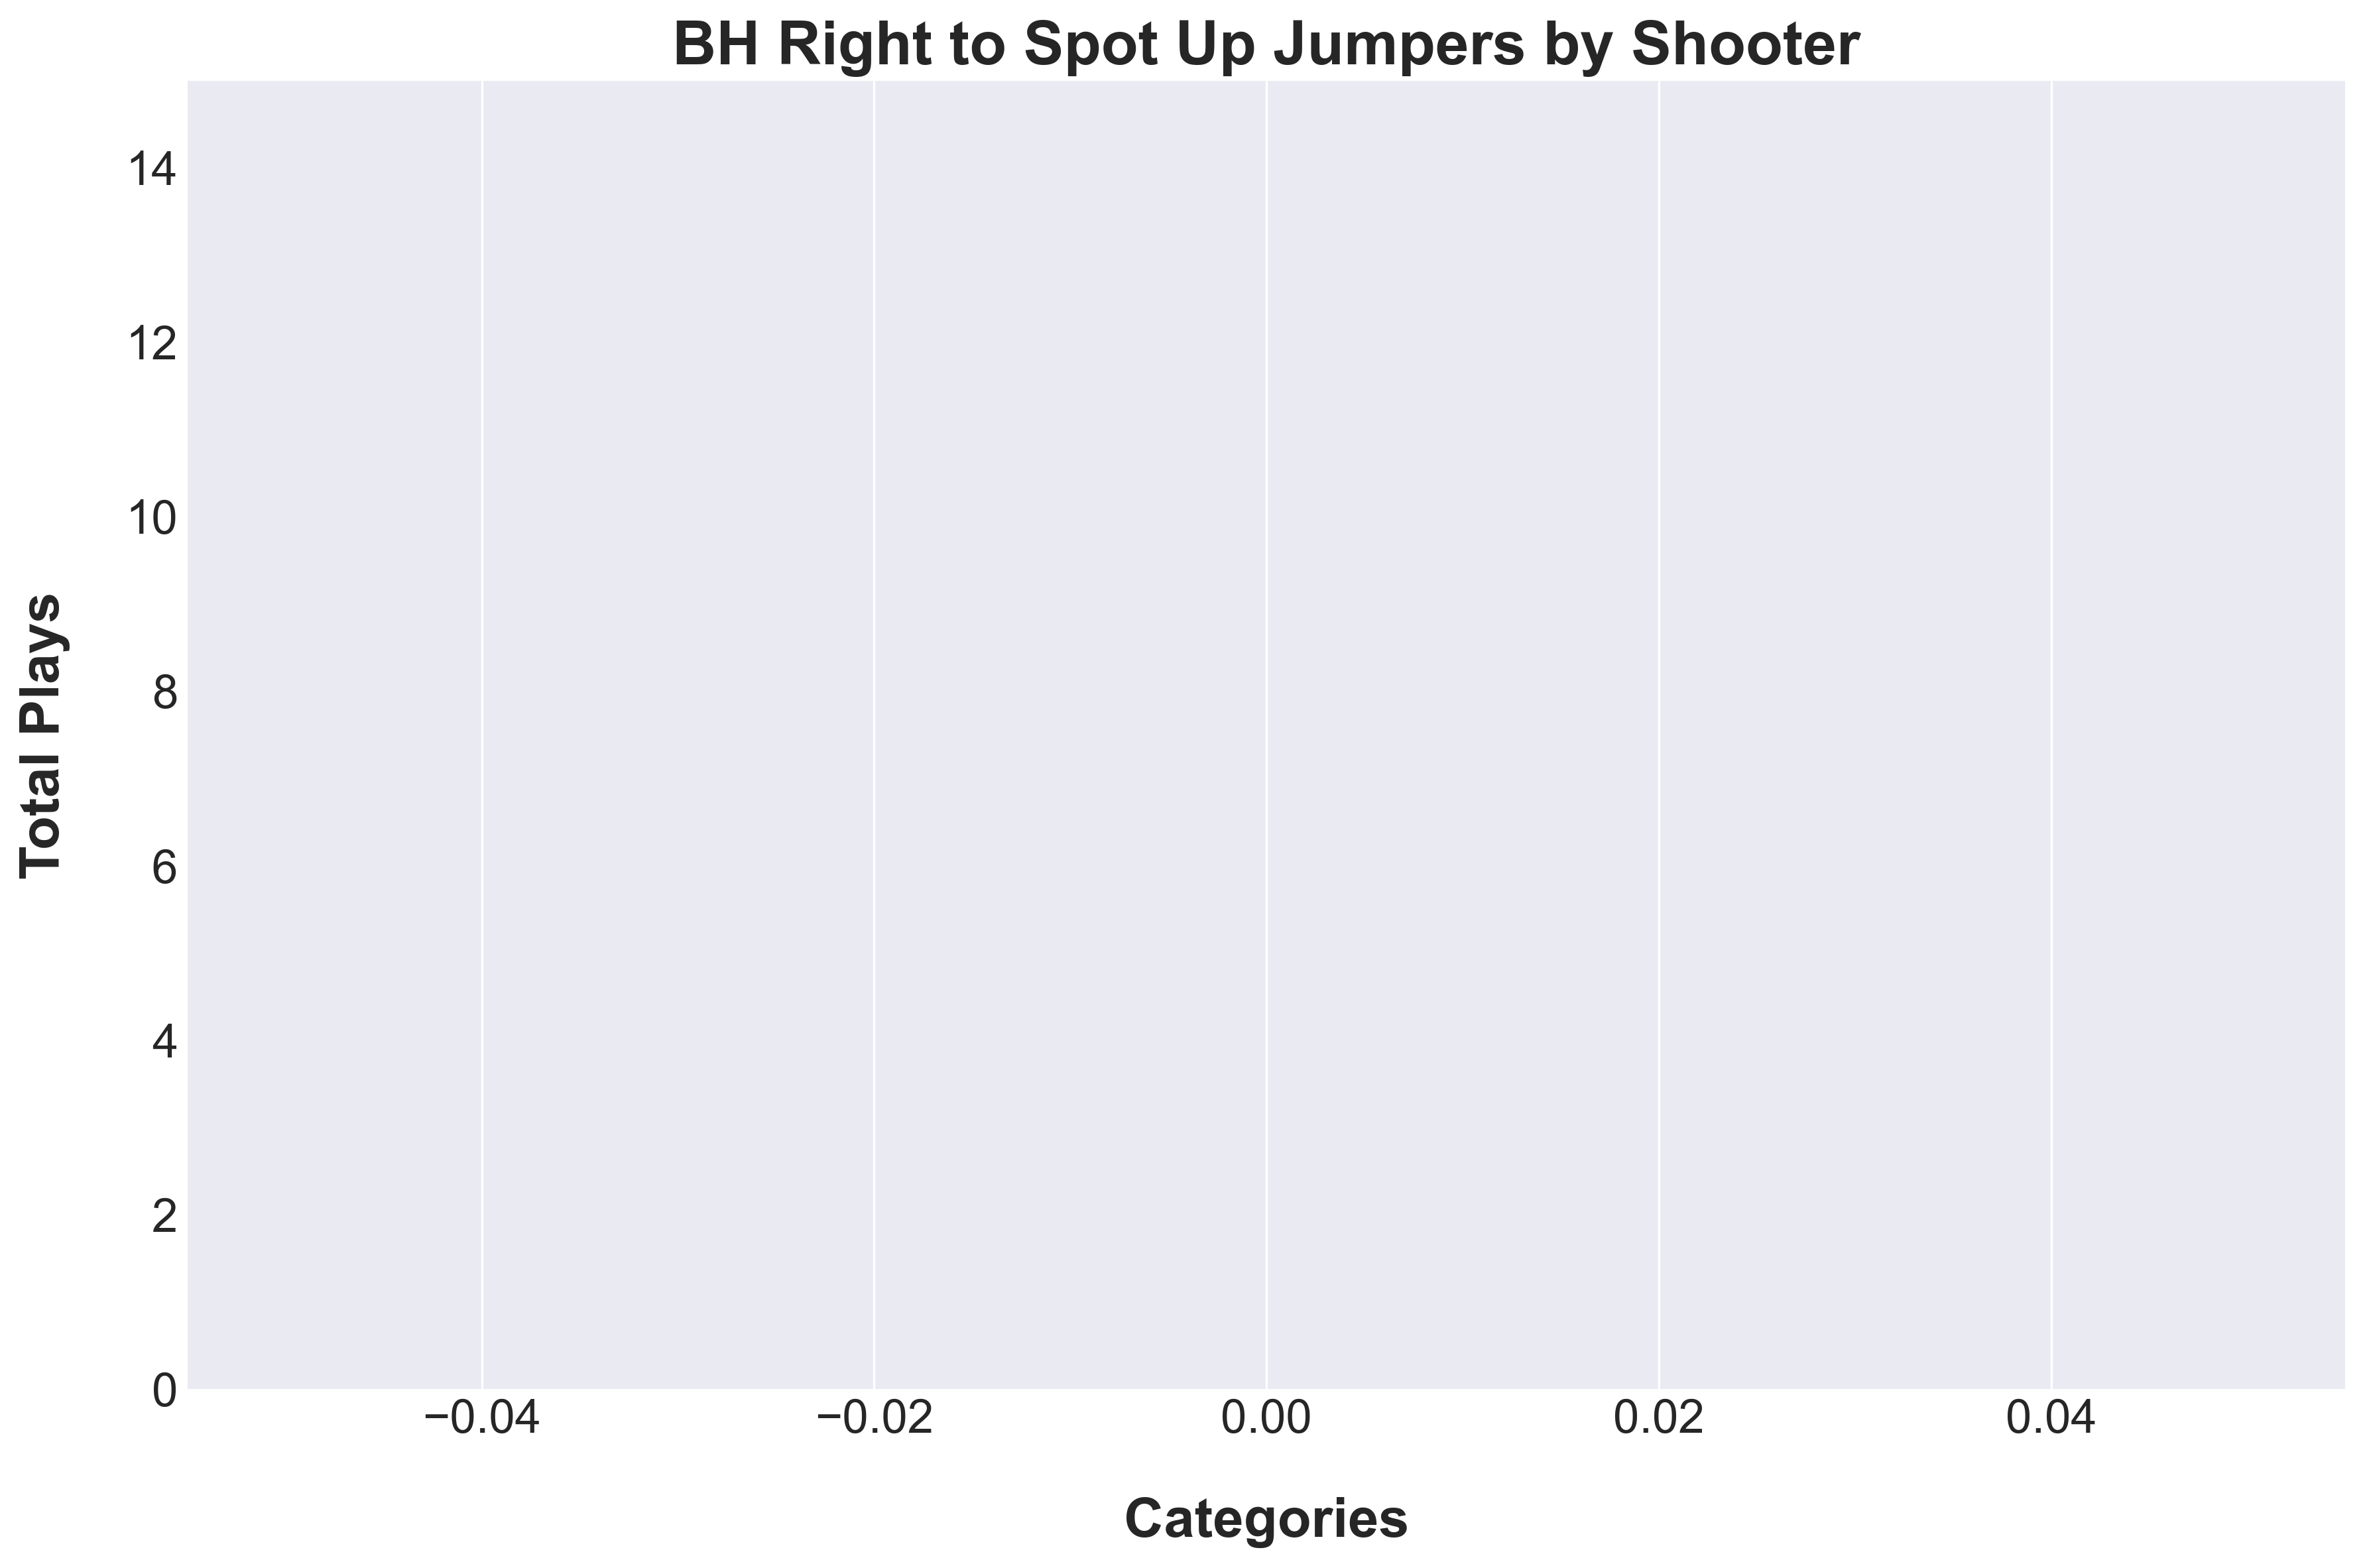
\includegraphics[width=\textwidth, height=.14\textheight]{images/PNR_PassRightShotsPlayer_Freq.png} % Adjust the width of the image to fit
    \end{minipage}
\end{table}

\vspace{-1em} % Add vertical space before the line (optional)
%\hrule height 1pt width 1\textwidth % Adjust height and width
\vspace{-1em} % Add vertical space after the line (optional)

% BH Right -> Rollman Rolls Secondary Player Stats
\begin{table}[H]
    \raisebox{3em}{ % Adjust this value to shift the tables vertically
    \begin{minipage}[t]{0.6\textwidth} % Left side (table) takes 85% of the width
        \flushleft
        \centering % Centering the title and the table
        \text{BH Right - Rollman Rolls Player Statistics} % Title above the table in bold
        \vskip .25em % Adds vertical space between title and table
        \scalebox{.6}{ % Scale the entire table down by half
            \renewcommand{\arraystretch}{1.4} % Adjust the number to increase or decrease row spacing
            \begin{tabular}{
            >{\centering\arraybackslash}p{3cm} 
            >{\centering\arraybackslash}p{.75cm} 
            >{\centering\arraybackslash}p{.75cm} 
            >{\centering\arraybackslash}p{.75cm} 
            >{\centering\arraybackslash}p{.75cm}
            >{\centering\arraybackslash}p{.75cm} 
            >{\centering\arraybackslash}p{.75cm}
            >{\centering\arraybackslash}p{.75cm}
            >{\centering\arraybackslash}p{.75cm} 
            >{\centering\arraybackslash}p{.75cm}}% Adjust column widths
            \toprule
            {\scriptsize \textbf{Player}} &
            {\scriptsize \textbf{Plays}} &
            {\scriptsize \textbf{2PA}} & 
            {\scriptsize \textbf{2PM}} & 
            {\scriptsize \textbf{2P\%}} & 
            {\scriptsize \textbf{MiA}} & 
            {\scriptsize \textbf{MiM}} &
            {\scriptsize \textbf{Mi\%}} &
            {\scriptsize \textbf{TO}} &
            {\scriptsize \textbf{Foul}} \\
            \midrule
            
                
            
                
            
                
            
                
            
                
            
                
            
                
            
                
            
                
            
                
            
                
            
                
            
                
            
                
            
                
            
                
            
                
            
                
            
                
            
                
            
                
            
                
                    
                        Kenny Wilburn & 
                        3 & 
                        3 & 
                        3 & 
                        100.0 & 
                        0 & 
                        0 & 
                        - & 
                        0 & 
                        0 \\
                    
                
            
                
            
                
            
                
            
                
            
                
            
                
            
                
            
                
            
                
            
                
            
                
            
                
            
                
            
                
            
                
            
                
            

            \bottomrule
        \end{tabular}
        } % End of \scalebox
    \end{minipage}
    } % End of raisebox, closing the adjustment
    \hfill % This adds some flexible space between the table and the image
    \begin{minipage}[c]{0.35\textwidth} % Right side (image) takes 10% of the width
        \flushright
        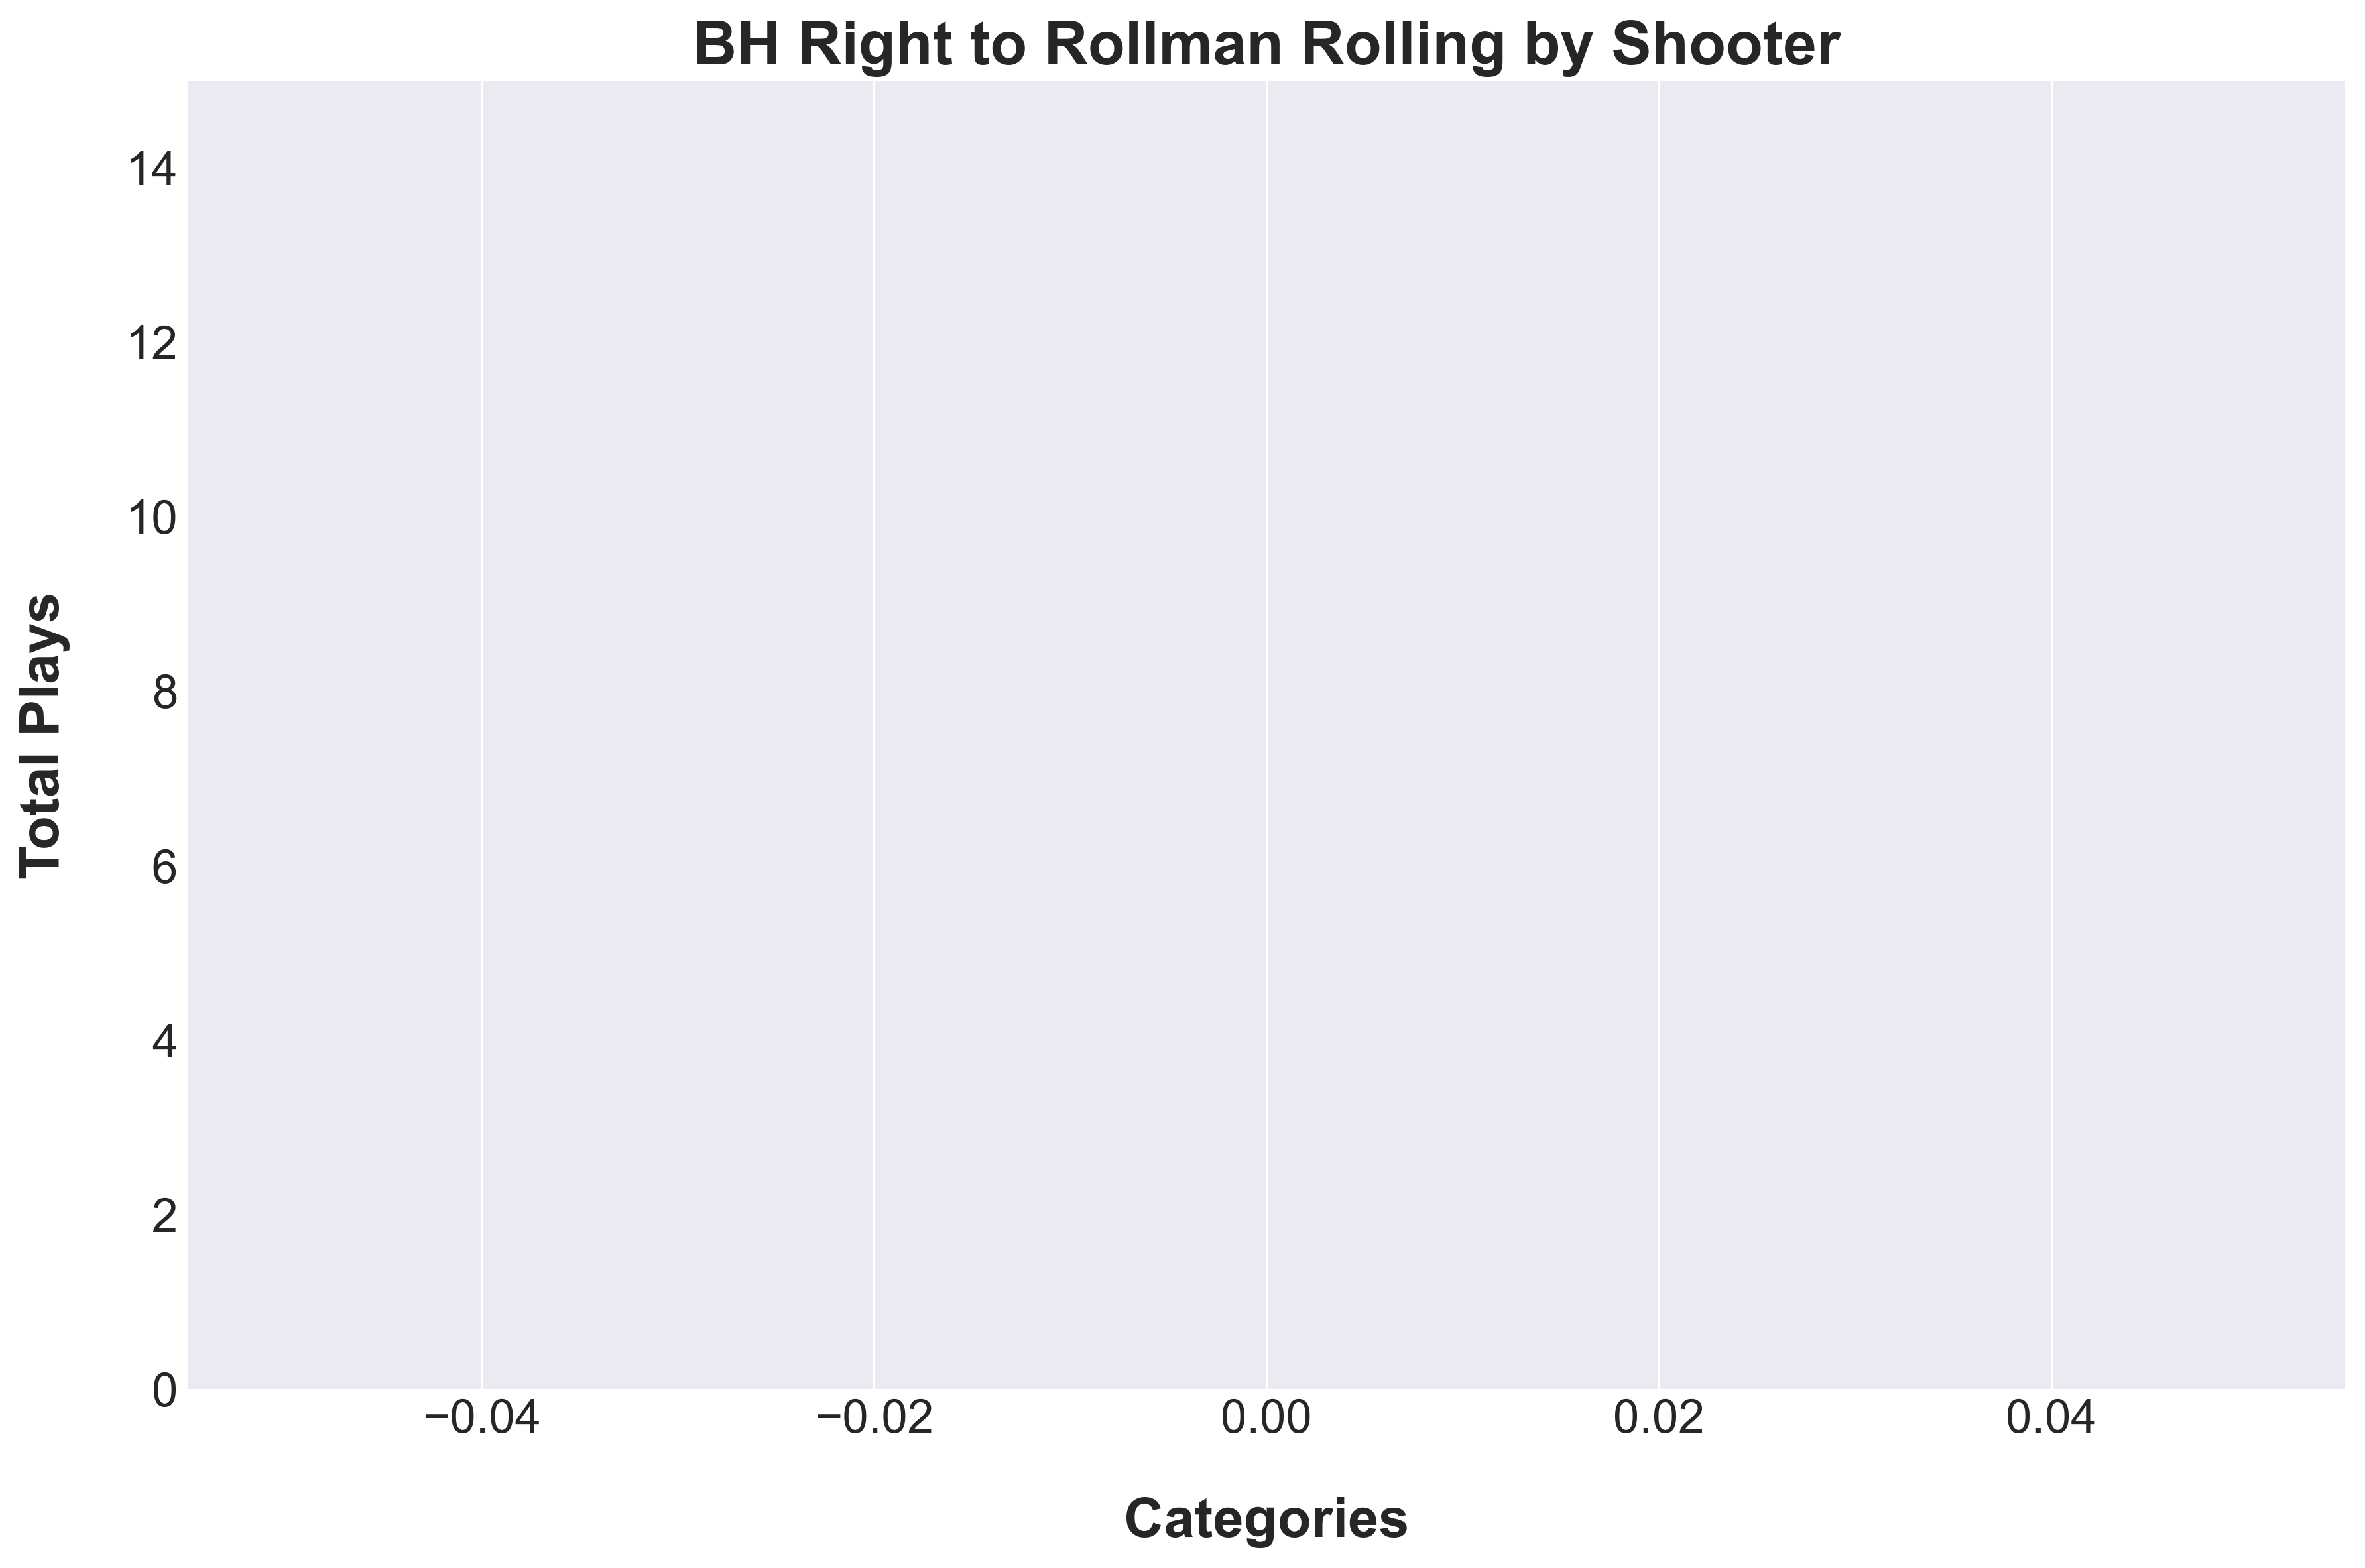
\includegraphics[width=\textwidth, height=.14\textheight]{images/PNR_PassRightRollsPlayer_Freq.png} % Adjust the width of the image to fit
    \end{minipage}
\end{table}

\vspace{-1em} % Add vertical space before the line (optional)
%\hrule height 1pt width 1\textwidth % Adjust height and width
\vspace{-1em} % Add vertical space after the line (optional)

% BH Right -> Rollman Slips Secondary Player Stats
\begin{table}[H]
    \raisebox{3em}{ % Adjust this value to shift the tables vertically
    \begin{minipage}[t]{0.6\textwidth} % Left side (table) takes 85% of the width
        \flushleft
        \centering % Centering the title and the table
        \text{BH Right - Rollman Slips Player Statistics} % Title above the table in bold
        \vskip .25em % Adds vertical space between title and table
        \scalebox{.55}{ % Scale the entire table down by half
            \renewcommand{\arraystretch}{1.4} % Adjust the number to increase or decrease row spacing
            \begin{tabular}{
            >{\centering\arraybackslash}p{3cm} 
            >{\centering\arraybackslash}p{.75cm} 
            >{\centering\arraybackslash}p{.75cm} 
            >{\centering\arraybackslash}p{.75cm} 
            >{\centering\arraybackslash}p{.75cm}
            >{\centering\arraybackslash}p{.75cm} 
            >{\centering\arraybackslash}p{.75cm} 
            >{\centering\arraybackslash}p{.75cm} 
            >{\centering\arraybackslash}p{.75cm}
            >{\centering\arraybackslash}p{.75cm} 
            >{\centering\arraybackslash}p{.75cm}
            >{\centering\arraybackslash}p{.75cm} 
            >{\centering\arraybackslash}p{.75cm}}% Adjust column widths
            \toprule
            {\scriptsize \textbf{Player}} &
            {\scriptsize \textbf{Plays}} &
            {\scriptsize \textbf{3PA}} &
            {\scriptsize \textbf{3PM}} &
            {\scriptsize \textbf{3P\%}} & 
            {\scriptsize \textbf{2PA}} & 
            {\scriptsize \textbf{2PM}} & 
            {\scriptsize \textbf{2P\%}} & 
            {\scriptsize \textbf{MiA}} & 
            {\scriptsize \textbf{MiM}} &
            {\scriptsize \textbf{Mi\%}} &
            {\scriptsize \textbf{TO}} &
            {\scriptsize \textbf{Foul}} \\
            \midrule
            
                
            
                
            
                
            
                
            
                
            
                
            
                
            
                
            
                
            
                
            
                
            
                
            
                
            
                
            
                
            
                
            
                
            
                
            
                
            
                
            
                
            
                
            
                
                    
                
            
                
            
                
            
                
            
                
            
                
            
                
            
                
            
                
            
                
            
                
            
                
            
                
            
                
            
                
            
                
            

            \bottomrule
        \end{tabular}
        } % End of \scalebox
    \end{minipage}
    } % End of raisebox, closing the adjustment
    \hfill % This adds some flexible space between the table and the image
    \begin{minipage}[c]{0.35\textwidth} % Right side (image) takes 10% of the width
        \flushright
        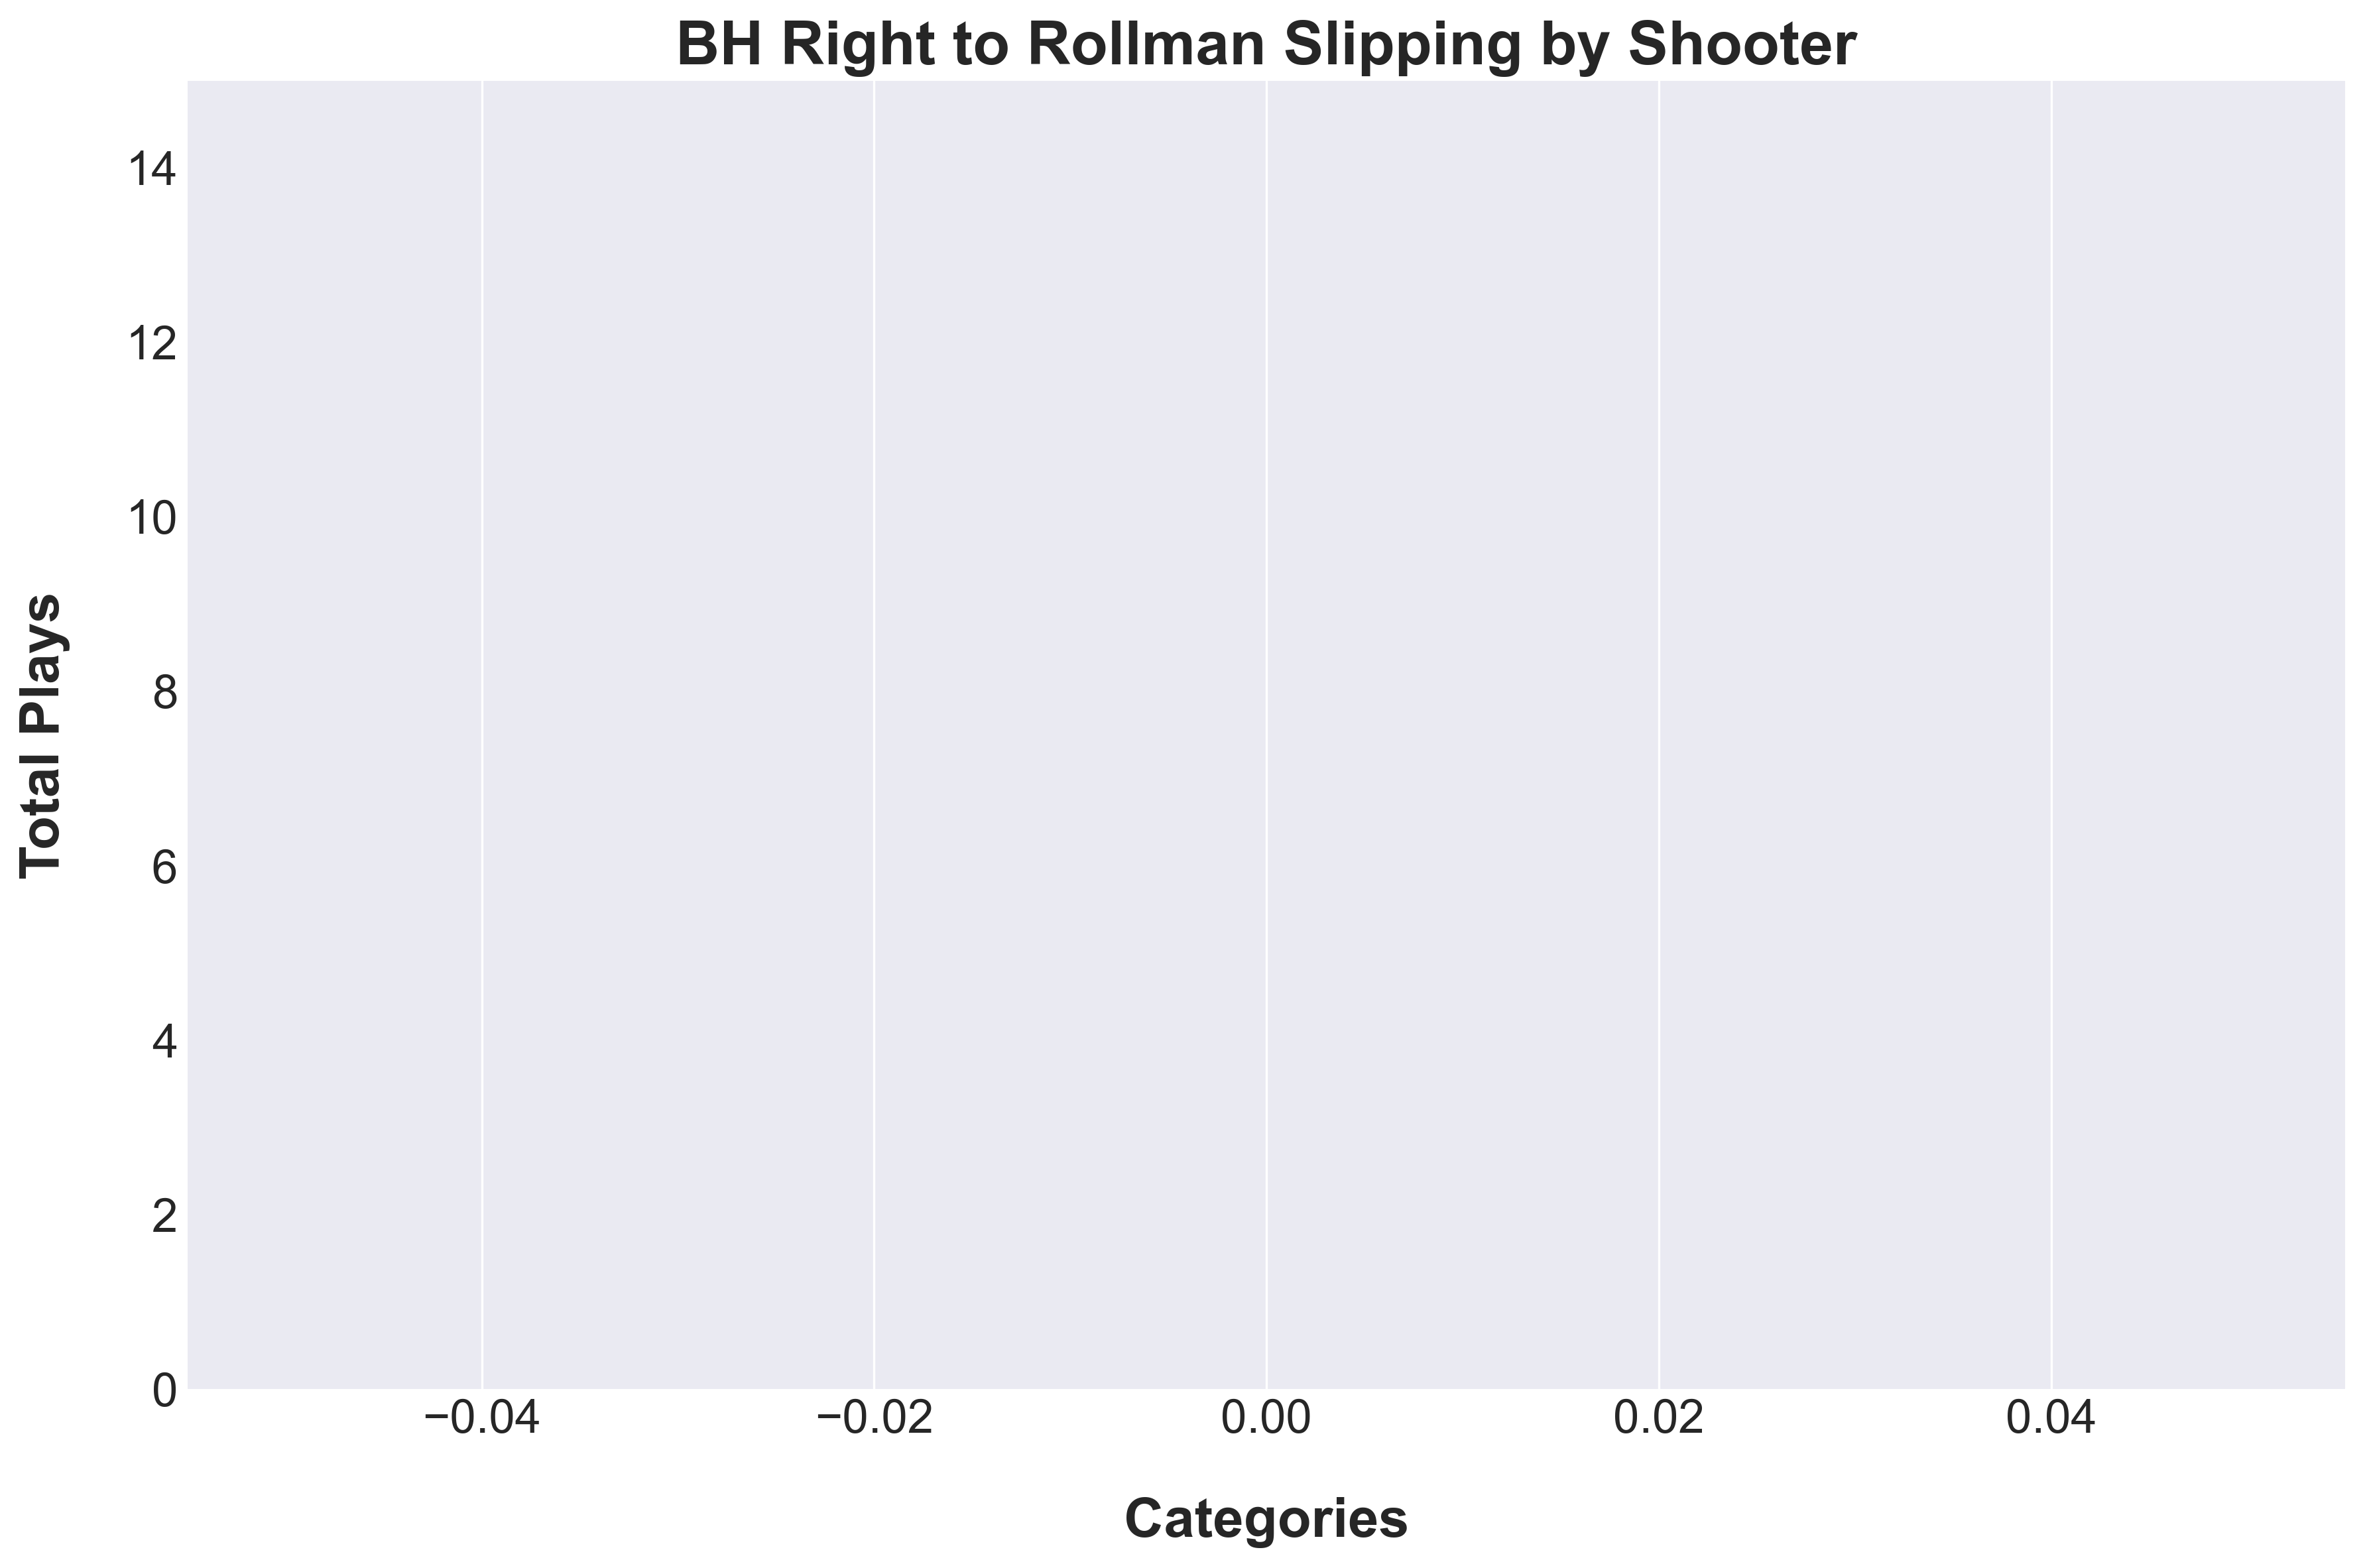
\includegraphics[width=\textwidth, height=.14\textheight]{images/PNR_PassRightSlipsPlayer_Freq.png} % Adjust the width of the image to fit
    \end{minipage}
\end{table}

\vspace{-1em} % Add vertical space before the line (optional)
%\hrule height 1pt width 1\textwidth % Adjust height and width
\vspace{-1em} % Add vertical space after the line (optional)

% BH Right -> Rollman Pops Secondary Player Stats
\begin{table}[H]
    \raisebox{3em}{ % Adjust this value to shift the tables vertically
    \begin{minipage}[t]{0.6\textwidth} % Left side (table) takes 85% of the width
        \flushleft
        \centering % Centering the title and the table
        \text{BH Right - Rollman Pops Player Statistics} % Title above the table in bold
        \vskip .25em % Adds vertical space between title and table
        \scalebox{.55}{ % Scale the entire table down by half
            \renewcommand{\arraystretch}{1.4} % Adjust the number to increase or decrease row spacing
            \begin{tabular}{
            >{\centering\arraybackslash}p{3cm} 
            >{\centering\arraybackslash}p{.75cm} 
            >{\centering\arraybackslash}p{.75cm} 
            >{\centering\arraybackslash}p{.75cm} 
            >{\centering\arraybackslash}p{.75cm}
            >{\centering\arraybackslash}p{.75cm} 
            >{\centering\arraybackslash}p{.75cm} 
            >{\centering\arraybackslash}p{.75cm} 
            >{\centering\arraybackslash}p{.75cm}
            >{\centering\arraybackslash}p{.75cm} 
            >{\centering\arraybackslash}p{.75cm}
            >{\centering\arraybackslash}p{.75cm} 
            >{\centering\arraybackslash}p{.75cm}}% Adjust column widths
            \toprule
            {\scriptsize \textbf{Player}} &
            {\scriptsize \textbf{Plays}} &
            {\scriptsize \textbf{3PA}} &
            {\scriptsize \textbf{3PM}} &
            {\scriptsize \textbf{3P\%}} & 
            {\scriptsize \textbf{2PA}} & 
            {\scriptsize \textbf{2PM}} & 
            {\scriptsize \textbf{2P\%}} & 
            {\scriptsize \textbf{MiA}} & 
            {\scriptsize \textbf{MiM}} &
            {\scriptsize \textbf{Mi\%}} &
            {\scriptsize \textbf{TO}} &
            {\scriptsize \textbf{Foul}} \\
            \midrule
            
                
            
                
            
                
            
                
            
                
            
                
            
                
            
                
            
                
            
                
            
                
            
                
            
                
            
                
            
                
            
                
            
                
            
                
            
                
            
                
            
                
            
                
            
                
            
                
                    
                        Josiah Turner & 
                        2 & 
                        0 & 
                        0 & 
                        - & 
                        1 & 
                        1 & 
                        100.0 & 
                        1 & 
                        1 & 
                        100.0 & 
                        0 & 
                        1 \\
                    
                        Kenny Wilburn & 
                        1 & 
                        0 & 
                        0 & 
                        - & 
                        1 & 
                        0 & 
                        0.0 & 
                        0 & 
                        0 & 
                        - & 
                        0 & 
                        0 \\
                    
                
            
                
            
                
            
                
            
                
            
                
            
                
            
                
            
                
            
                
            
                
            
                
            
                
            
                
            
                
            

            \bottomrule
        \end{tabular}
        } % End of \scalebox
    \end{minipage}
    } % End of raisebox, closing the adjustment
    \hfill % This adds some flexible space between the table and the image
    \begin{minipage}[c]{0.35\textwidth} % Right side (image) takes 10% of the width
        \flushright
        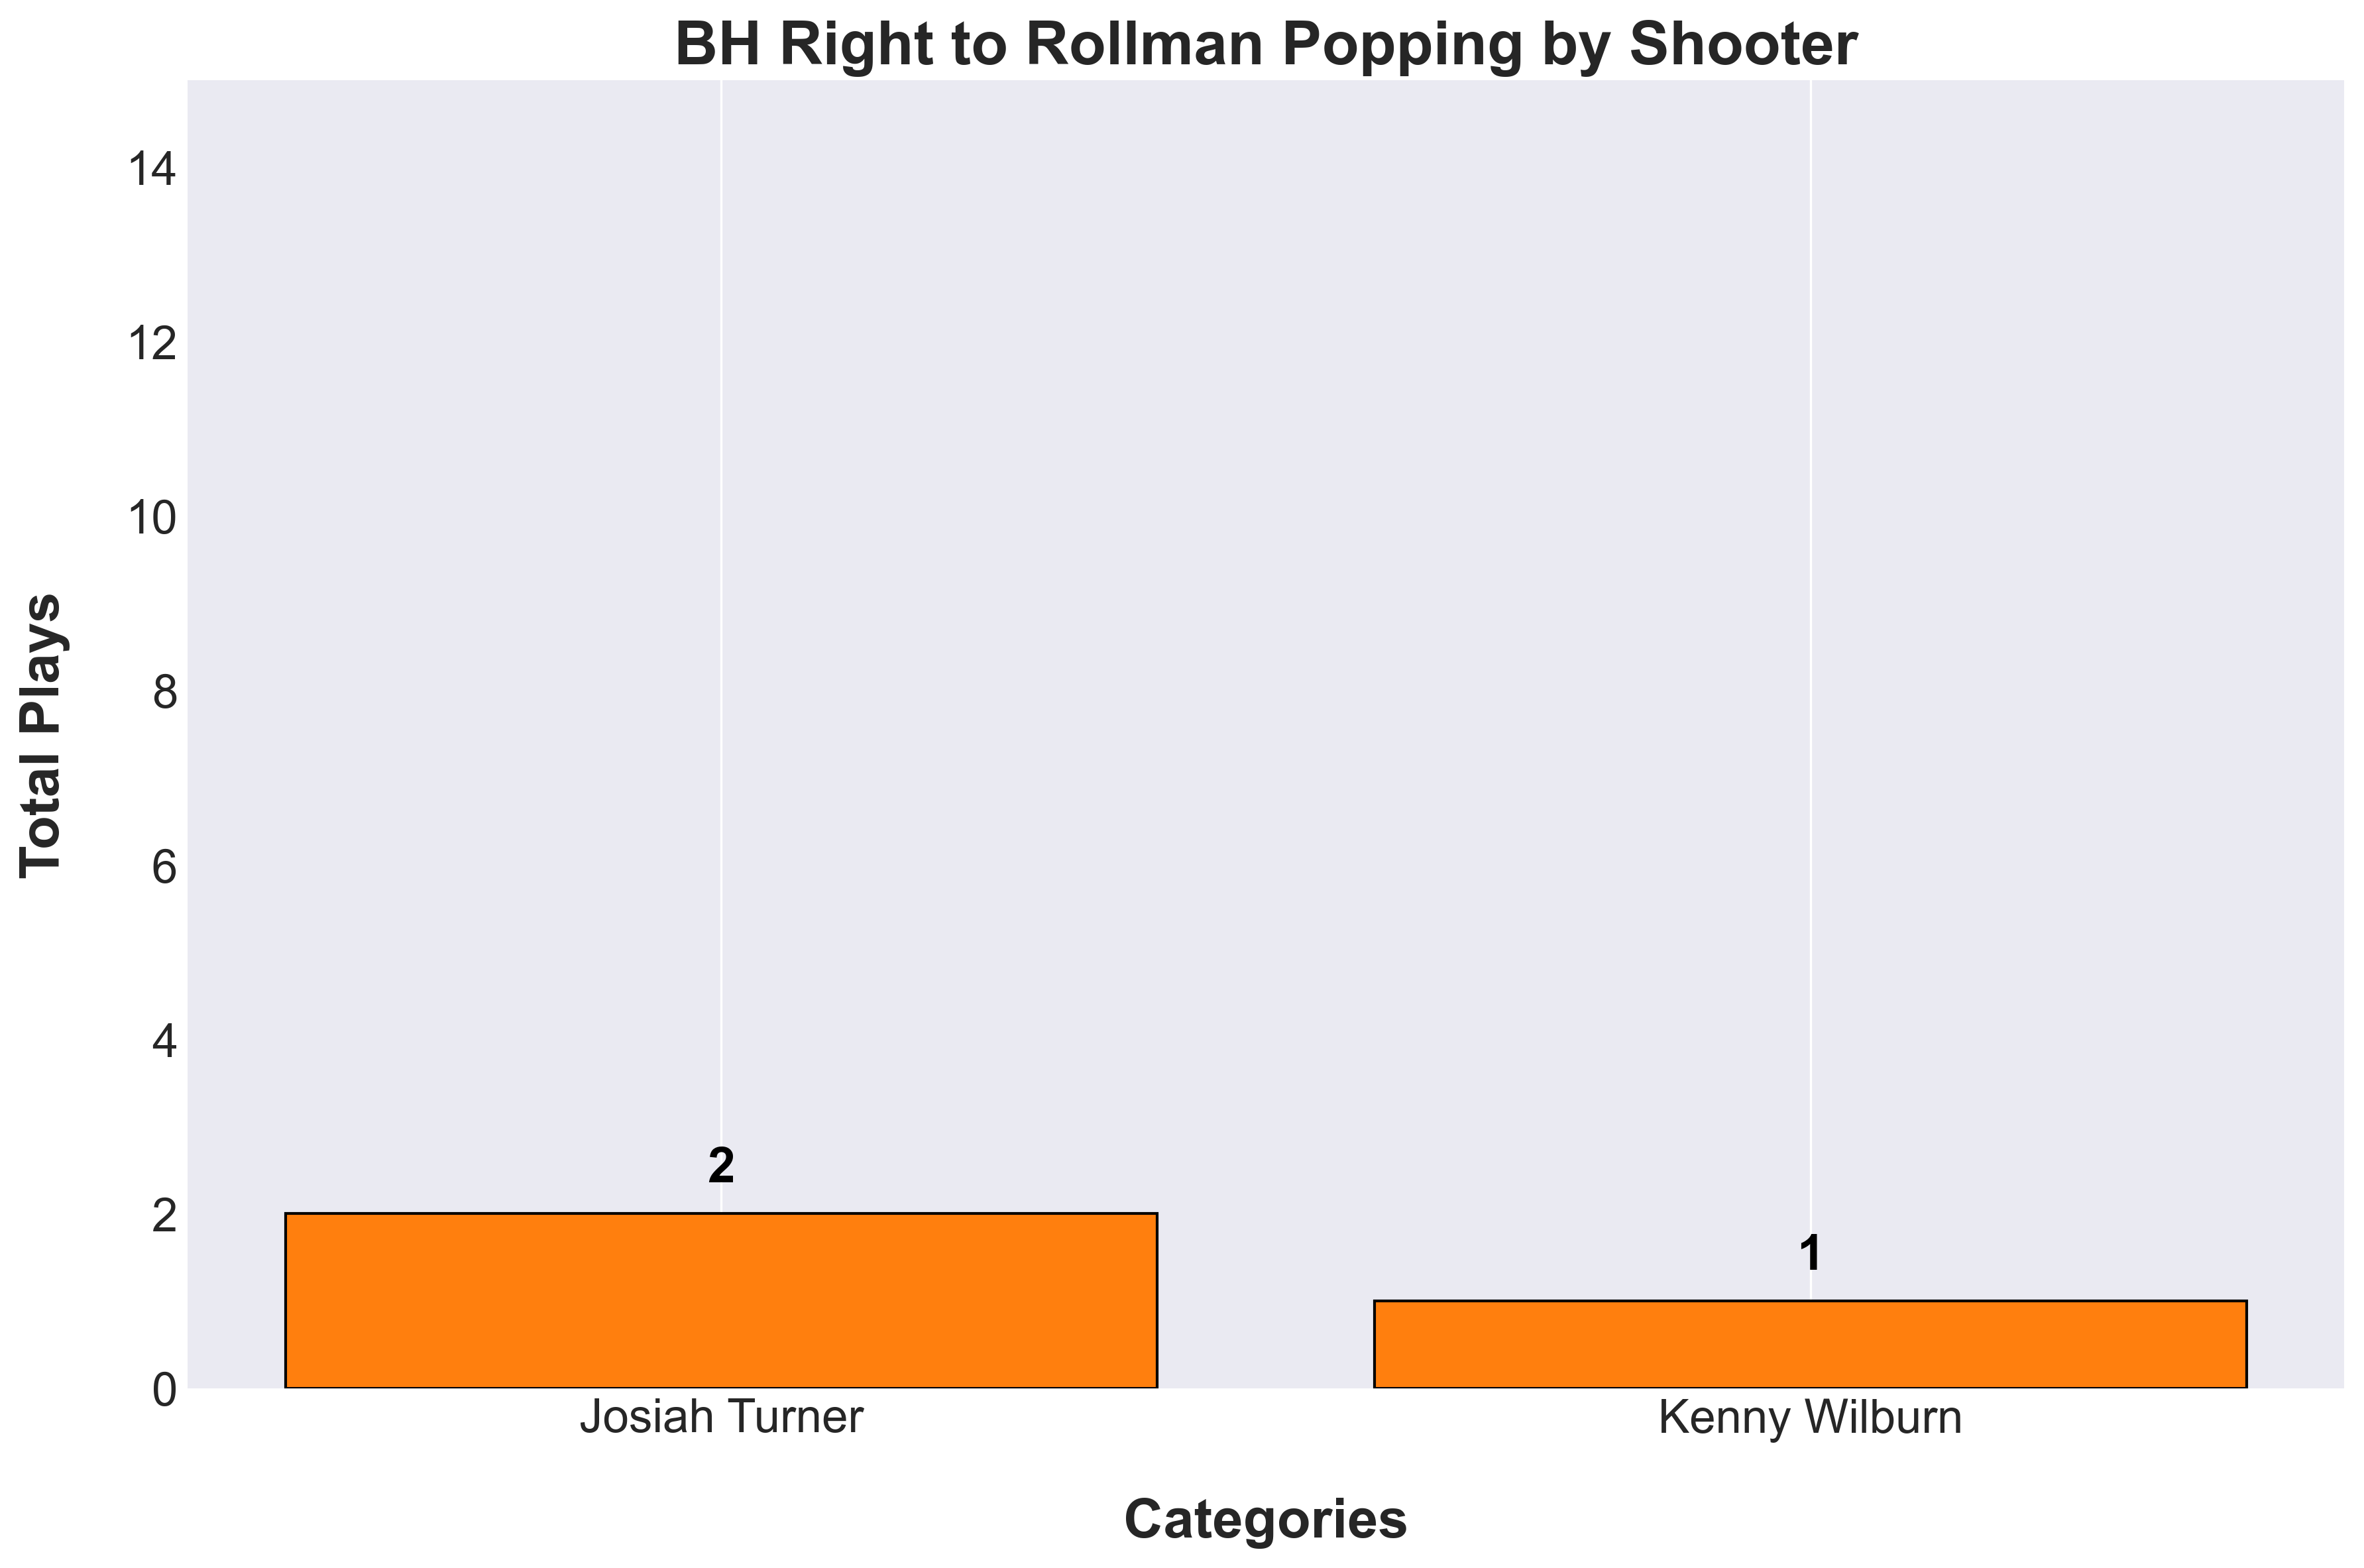
\includegraphics[width=\textwidth, height=.14\textheight]{images/PNR_PassRightPopsPlayer_Freq.png} % Adjust the width of the image to fit
    \end{minipage}
\end{table}

\vspace{-1em} % Add vertical space before the line (optional)
\hrule height 1pt width 1\textwidth % Adjust height and width
\vspace{1em} % Add vertical space after the line (optional)

\clearpage

% ----------------------
% Post Ups Visuals and Insights Section
% ----------------------
\subsection{Post-Ups}

\vspace{1.25em} % Add vertical space before the line (optional)
\textbf{Key Notes on Post Up Tendencies}
\vspace{0.5em} % Add space between the title and the itemized list

\begin{itemize}
    \item Post Ups make up x\% of players offensive load
    \vspace{0.3em} % Add space between the title and the itemized list
    \item Player is more efficient shooting over his left shoulder and get shots off of the left block x\% of the time which is much higher than the middle and right block.
\end{itemize}

\vspace{1em} % Add vertical space before the line (optional)
\hrule height 1pt width 1\textwidth % Adjust height and width
\vspace{0em} % Add vertical space after the line (optional)

\subsubsection{Post Shot Statistics}

% All Post Up Statistics Table w/ room for insights
\begin{table}[H]
    \centering
    \begin{minipage}[t]{0.6\textwidth} % Left side (table) takes 85% of the width
        %\flushright
        \centering % Centering the title and the table
        \text{Total Post Shot Statistics} % Title above the table in bold
        \vskip .25em % Adds vertical space between title and table
        \scalebox{.85}{ % Scale the entire table down by half
            \scriptsize % Reduce the font size
            \begin{tabular}{
            >{\centering\arraybackslash}p{.75cm} 
            >{\centering\arraybackslash}p{.5cm} 
            >{\centering\arraybackslash}p{.5cm} 
            >{\centering\arraybackslash}p{.5cm}
            >{\centering\arraybackslash}p{.5cm} 
            >{\centering\arraybackslash}p{.5cm} 
            >{\centering\arraybackslash}p{.5cm}
            >{\centering\arraybackslash}p{.5cm} 
            >{\centering\arraybackslash}p{.5cm}}% Adjust column widths
            \toprule
            \textbf{Plays} &
            \textbf{2PA} & 
            \textbf{2PM} & 
            \textbf{2P\%} & 
            \textbf{MiA} & 
            \textbf{MiM} &
            \textbf{Mi\%} &
            \textbf{TO} &
            \textbf{Foul} \\
            \midrule
            
                
            
                
            
                
            
                
            
                
            
                
                    2 &
                    1 & 1 &
                    100.0 &
                    0 & 0 &
                    - &
                    0 & 1 \\
                
            
                
            
                
            
                
            
                
            
                
            
                
            
                
            
                
            
                
            
                
            
                
            
                
            
                
            
                
            
                
            
                
            
                
            


            \bottomrule
            \end{tabular}
        }
    \end{minipage}
\end{table}

\vspace{0em} % Add vertical space before the line (optional)
%\hrule height 1pt width 1\textwidth % Adjust height and width
\vspace{-1em} % Add vertical space after the line (optional)

% Post Stats of where player shoots from Middle vs Left Block vs Right Block
\begin{table}[H]
    \raisebox{3em}{ % Adjust this value to shift the tables vertically
    \begin{minipage}[t]{0.6\textwidth} % Left side (table) takes 85% of the width
        \flushleft
        \centering % Centering the title and the table
        \text{Post Up Location Statistics} % Title above the table in bold
        \vskip .25em % Adds vertical space between title and table
        \scalebox{.6}{ % Scale the entire table down by half
            \renewcommand{\arraystretch}{1.4} % Adjust the number to increase or decrease row spacing
            \begin{tabular}{
            >{\centering\arraybackslash}p{2.5cm} 
            >{\centering\arraybackslash}p{.75cm} 
            >{\centering\arraybackslash}p{.75cm} 
            >{\centering\arraybackslash}p{.75cm} 
            >{\centering\arraybackslash}p{.75cm}
            >{\centering\arraybackslash}p{.75cm} 
            >{\centering\arraybackslash}p{.75cm}
            >{\centering\arraybackslash}p{.75cm}
            >{\centering\arraybackslash}p{.75cm} 
            >{\centering\arraybackslash}p{.75cm}}% Adjust column widths
            \toprule
            {\scriptsize \textbf{Location}} &
            {\scriptsize \textbf{Plays}} &
            {\scriptsize \textbf{2PA}} & 
            {\scriptsize \textbf{2PM}} & 
            {\scriptsize \textbf{2P\%}} & 
            {\scriptsize \textbf{MiA}} & 
            {\scriptsize \textbf{MiM}} &
            {\scriptsize \textbf{Mi\%}} &
            {\scriptsize \textbf{TO}} &
            {\scriptsize \textbf{Foul}} \\
            \midrule
            
                
            
                
            
                
            
                
            
                
            
                
            
                
            
                
                    Left Block & 2 &
                    1 & 1 &
                    100.0 &
                    0 & 0 &
                    - &
                    0 & 1 \\
                
            
                
            
                
            
                
            
                
            
                
            
                
            
                
            
                
            
                
            
                
            
                
            
                
            
                
            
                
            
                
            


            \bottomrule
        \end{tabular}
        } % End of \scalebox
    \end{minipage}
    } % End of raisebox, closing the adjustment
    \hfill % This adds some flexible space between the table and the image
    \begin{minipage}[c]{0.35\textwidth} % Right side (image) takes 10% of the width
        \flushright
        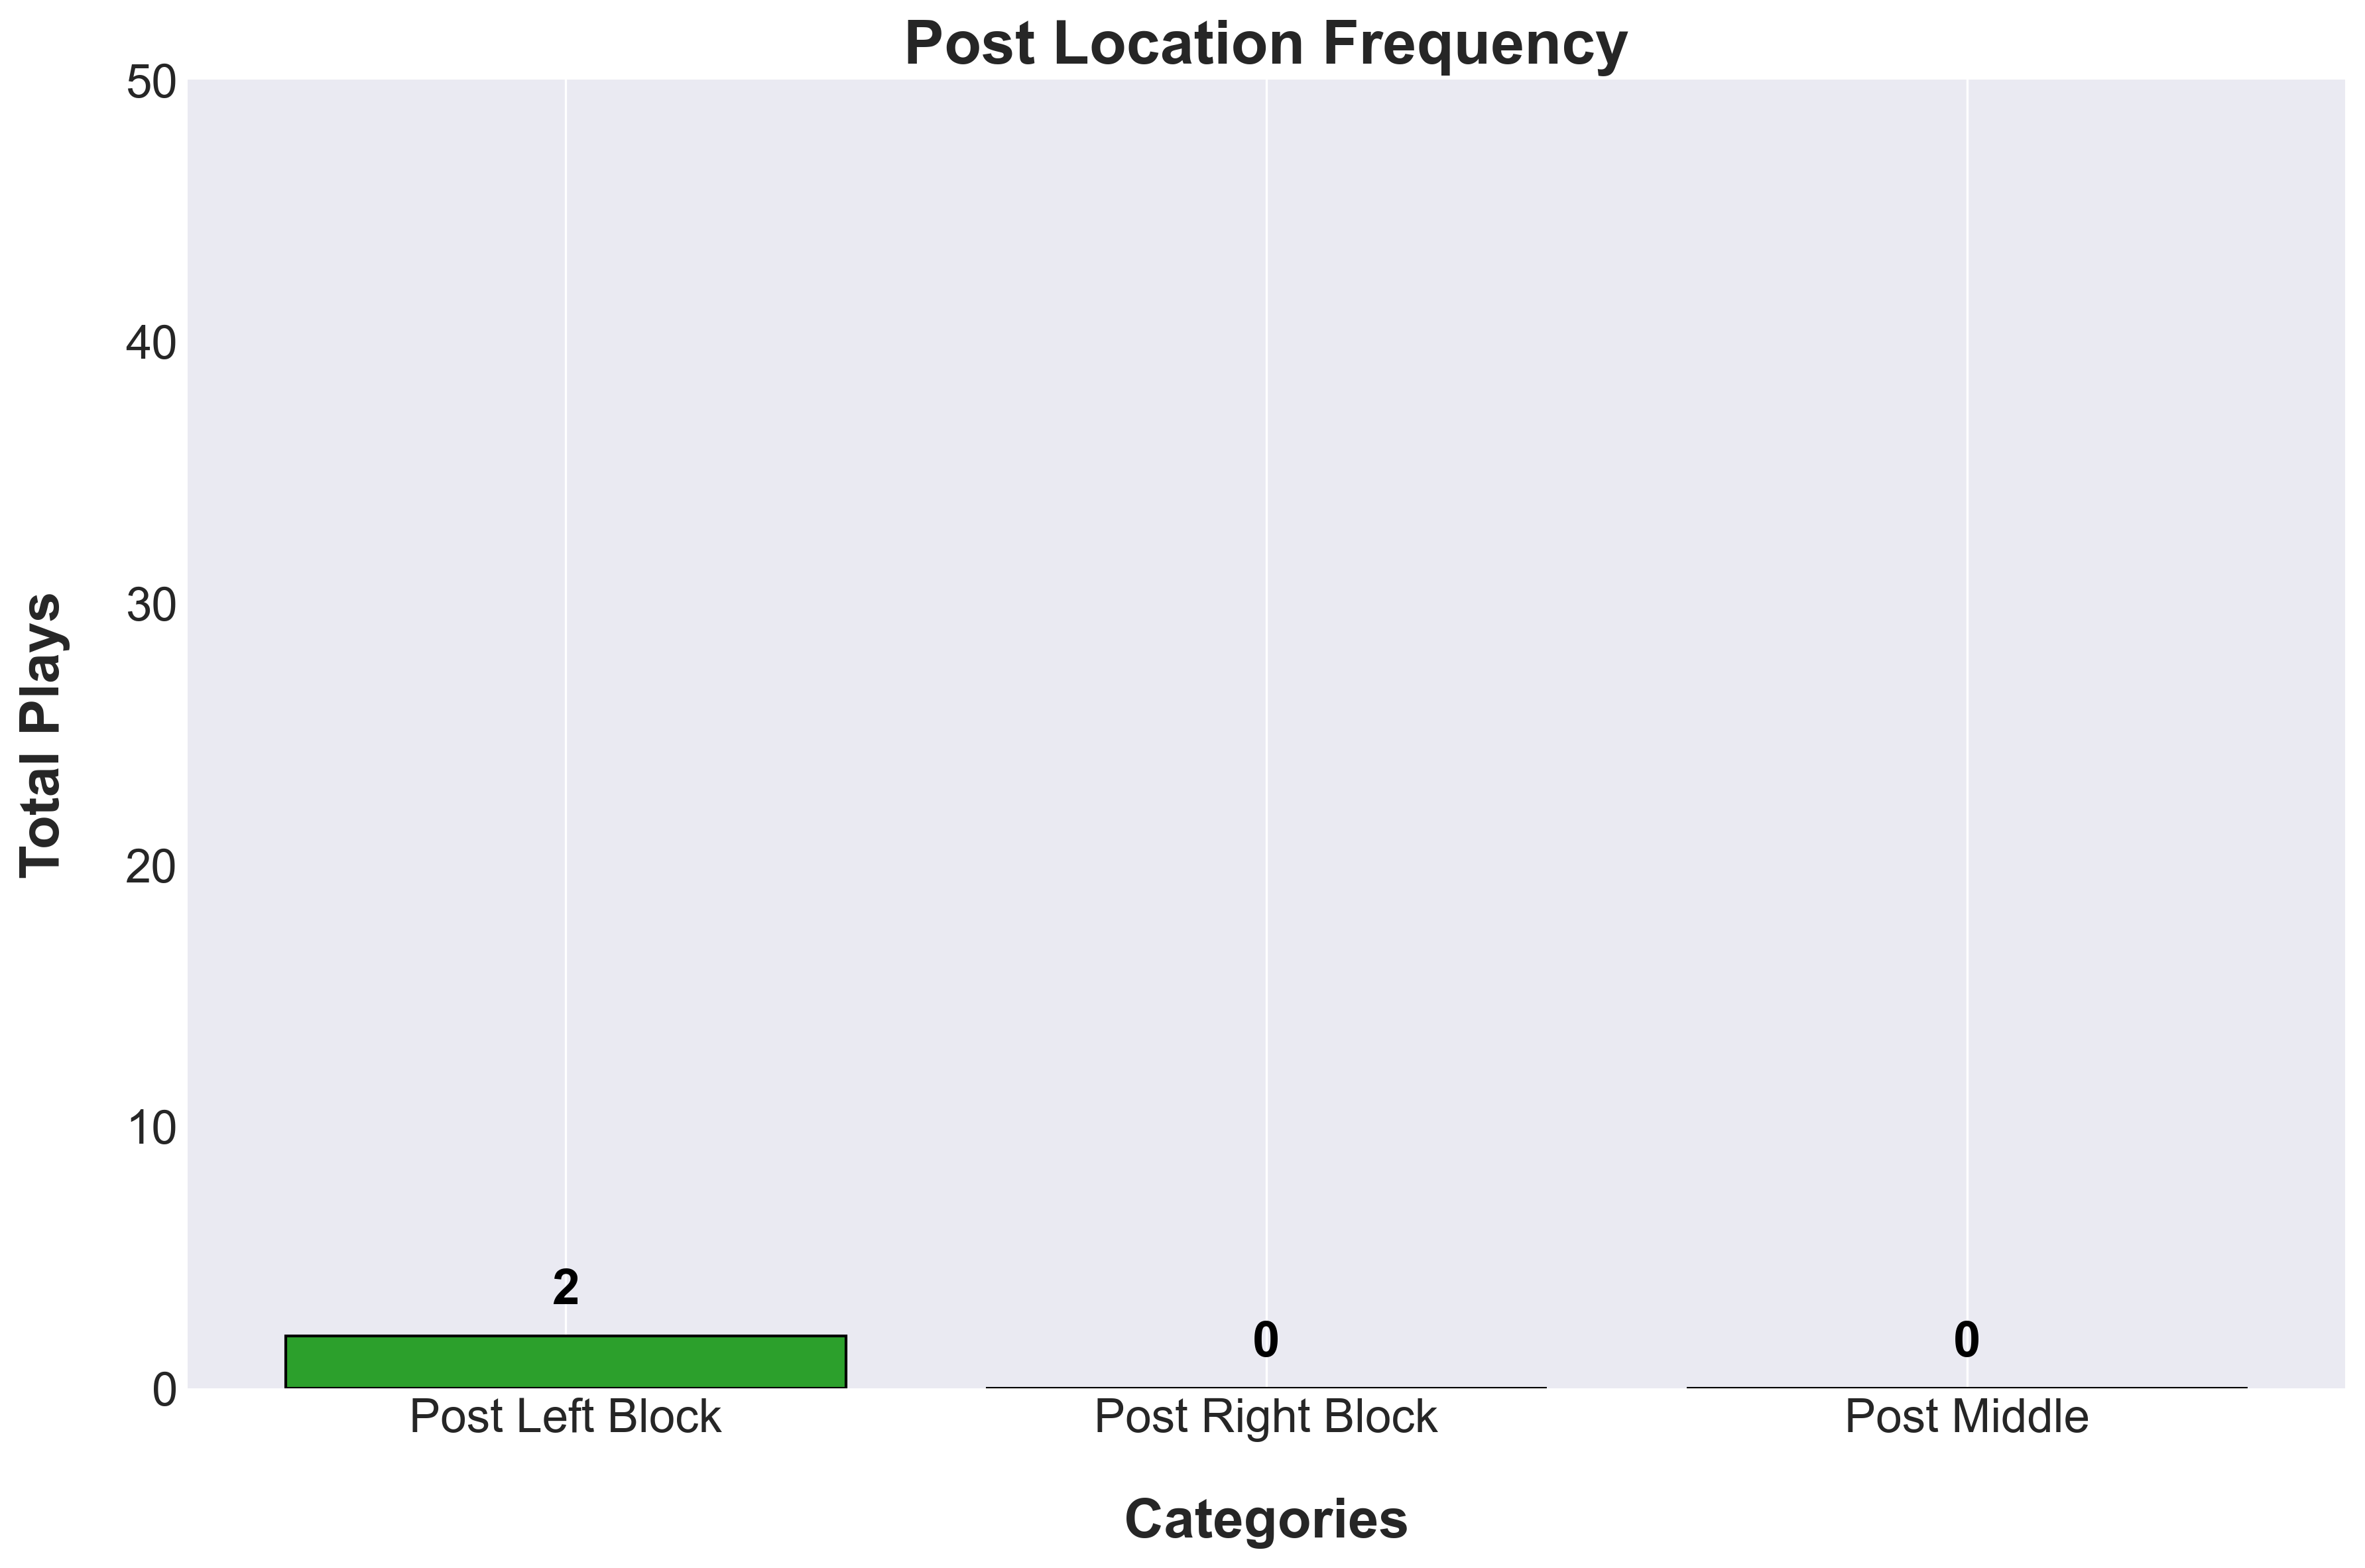
\includegraphics[width=\textwidth, height=.14\textheight]{images/Post_Location_Freq.png} % Adjust the width of the image to fit
    \end{minipage}
\end{table}

\vspace{-1em} % Add vertical space before the line (optional)
%\hrule height 1pt width 1\textwidth % Adjust height and width
\vspace{-1em} % Add vertical space after the line (optional)

% Post Shot Type Statistics
\begin{table}[H]
    \raisebox{3.5em}{ % Adjust this value to shift the tables vertically
    \begin{minipage}[t]{0.6\textwidth} % Left side (table) takes 85% of the width
        \flushleft
        \centering % Centering the title and the table
        \text{Post Shot Type Statistics} % Title above the table in bold
        \vskip .25em % Adds vertical space between title and table
        \scalebox{.6}{ % Scale the entire table down by half
            \renewcommand{\arraystretch}{1.4} % Adjust the number to increase or decrease row spacing
            \begin{tabular}{
            >{\centering\arraybackslash}p{2.75cm} 
            >{\centering\arraybackslash}p{.75cm} 
            >{\centering\arraybackslash}p{.75cm} 
            >{\centering\arraybackslash}p{.75cm} 
            >{\centering\arraybackslash}p{.75cm}
            >{\centering\arraybackslash}p{.75cm} 
            >{\centering\arraybackslash}p{.75cm}
            >{\centering\arraybackslash}p{.75cm}
            >{\centering\arraybackslash}p{.75cm} 
            >{\centering\arraybackslash}p{.75cm}}% Adjust column widths
            \toprule
            {\scriptsize \textbf{Shot Type}} &
            {\scriptsize \textbf{Plays}} &
            {\scriptsize \textbf{2PA}} & 
            {\scriptsize \textbf{2PM}} & 
            {\scriptsize \textbf{2P\%}} & 
            {\scriptsize \textbf{MiA}} & 
            {\scriptsize \textbf{MiM}} &
            {\scriptsize \textbf{Mi\%}} &
            {\scriptsize \textbf{TO}} &
            {\scriptsize \textbf{Foul}} \\
            \midrule
            
                
            
                
            
                
            
                
            
                
            
                
            
                
            
                
            
                
            
                
            
                
            
                
                    Left Shoulder & 1 &
                    0 & 0 &
                    - &
                    0 & 0 &
                    - &
                    0 & 1 \\
                
            
                
                    Right Shoulder & 1 &
                    1 & 1 &
                    100.0 &
                    0 & 0 &
                    - &
                    0 & 0 \\
                
            
                
            
                
            
                
            
                
            
                
            
                
            
                
            
                
            
                
            
                
            


            \bottomrule
        \end{tabular}
        } % End of \scalebox
    \end{minipage}
    } % End of raisebox, closing the adjustment
    \hfill
    \begin{minipage}[c]{0.35\textwidth} % Right side (image) takes 10% of the width
        \flushright
        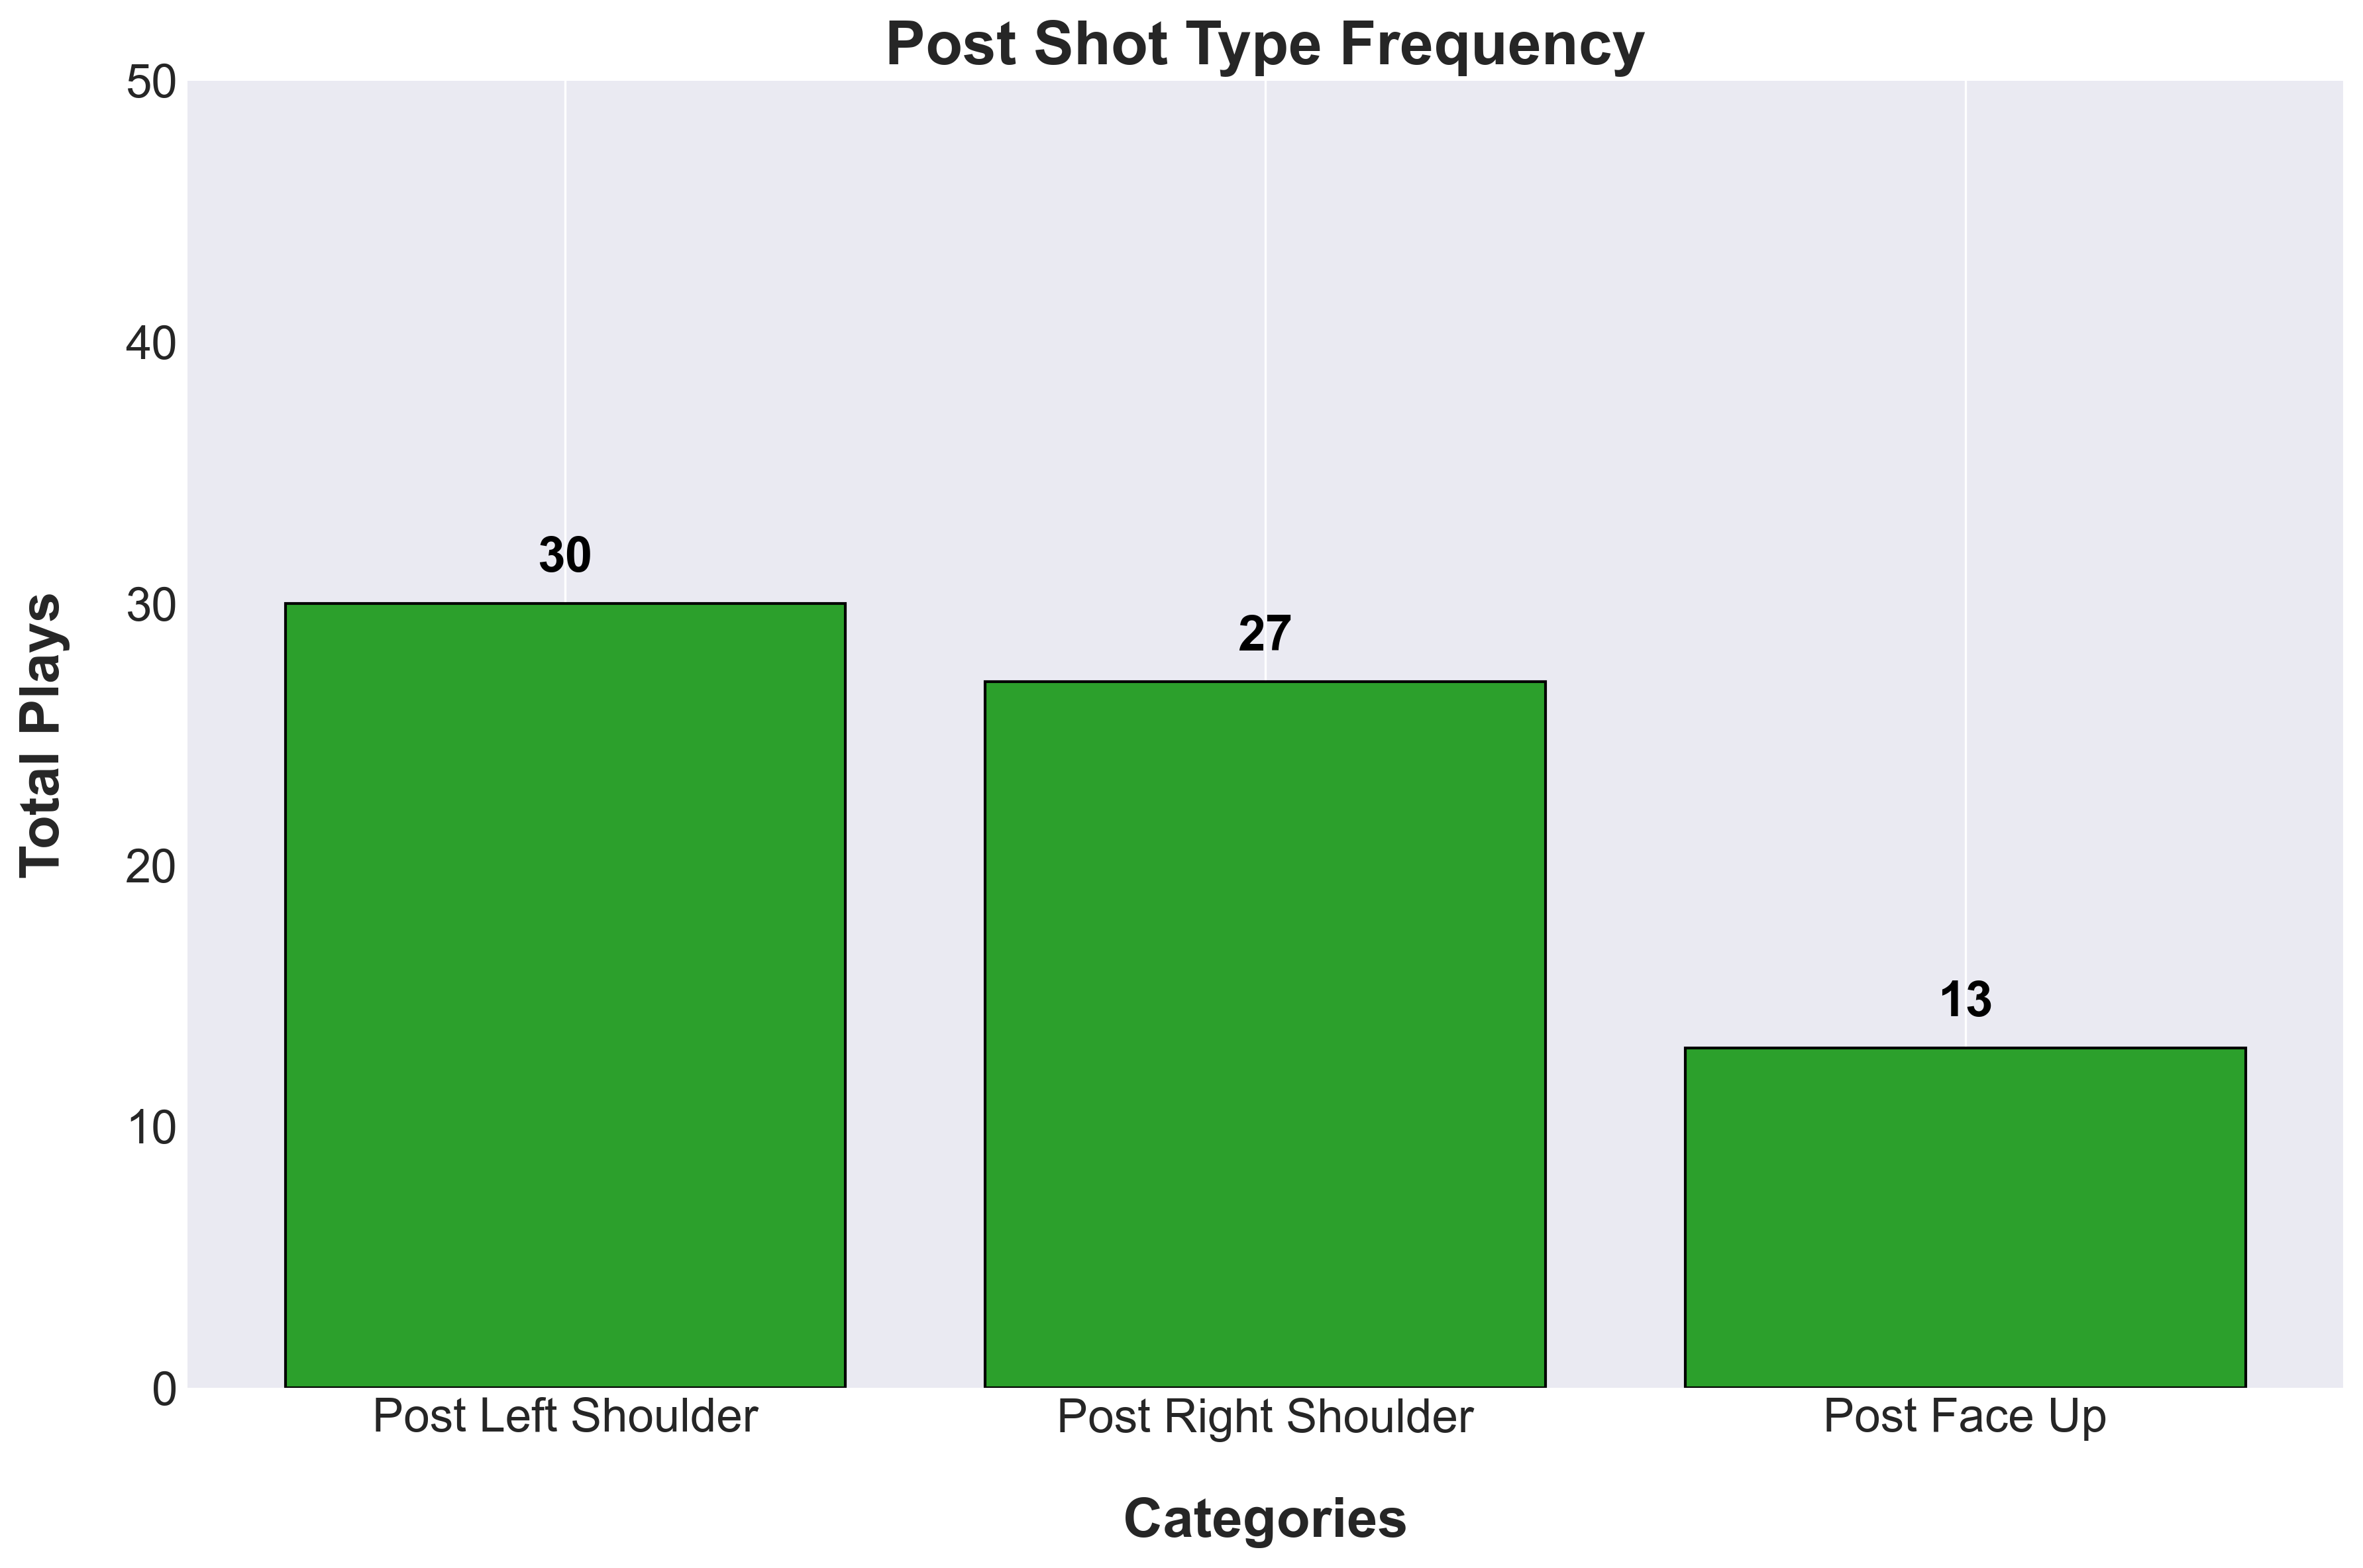
\includegraphics[width=\textwidth, height=.14\textheight]{images/Post_ShotType_Freq.png} % Adjust the width of the image to fit
    \end{minipage}
    
\end{table}

\vspace{-1em} % Add vertical space before the line (optional)
%\hrule height 1pt width 1\textwidth % Adjust height and width
\vspace{-1em} % Add vertical space after the line (optional)

% Post Stats for Combination of Location and Shot Type Stats
\begin{table}[H]
    \raisebox{6em}{ % Adjust this value to shift the tables vertically
    \begin{minipage}[t]{0.6\textwidth} % Left side (table) takes 85% of the width
        \flushleft
        \centering % Centering the title and the table
        \text{Post Combination Statistics} % Title above the table in bold
        \vskip .25em % Adds vertical space between title and table
        \scalebox{.6}{ % Scale the entire table down by half
            \renewcommand{\arraystretch}{1.4} % Adjust the number to increase or decrease row spacing
            \begin{tabular}{
            >{\centering\arraybackslash}p{5.5cm} 
            >{\centering\arraybackslash}p{.75cm} 
            >{\centering\arraybackslash}p{.75cm} 
            >{\centering\arraybackslash}p{.75cm} 
            >{\centering\arraybackslash}p{.75cm}
            >{\centering\arraybackslash}p{.75cm} 
            >{\centering\arraybackslash}p{.75cm} 
            >{\centering\arraybackslash}p{.75cm}
            >{\centering\arraybackslash}p{.75cm} 
            >{\centering\arraybackslash}p{.75cm}}% Adjust column widths
            \toprule
            {\scriptsize \textbf{PlayType}} &
            {\scriptsize \textbf{Plays}} &
            {\scriptsize \textbf{2PA}} & 
            {\scriptsize \textbf{2PM}} & 
            {\scriptsize \textbf{2P\%}} & 
            {\scriptsize \textbf{MiA}} & 
            {\scriptsize \textbf{MiM}} &
            {\scriptsize \textbf{Mi\%}} &
            {\scriptsize \textbf{TO}} &
            {\scriptsize \textbf{Foul}} \\
            \midrule
            
                
            
                
            
                
            
                
            
                
            
                
            
                
            
                
            
                
            
                
            
                
            
                
            
                
            
                
            
                
            
                
                    Left Block - Left Shoulder & 1 &
                    0 & 0 &
                    - &
                    0 & 0 &
                    - &
                    0 & 1 \\
                
            
                
                    Left Block - Right Shoulder & 1 &
                    1 & 1 &
                    100.0 &
                    0 & 0 &
                    - &
                    0 & 0 \\
                
            
                
            
                
            
                
            
                
            
                
            
                
            


            \bottomrule
        \end{tabular}
        } % End of \scalebox
    \end{minipage}
    } % End of raisebox, closing the adjustment
    \hfill % This adds some flexible space between the table and the image
    \begin{minipage}[c]{0.35\textwidth} % Right side (image) takes 10% of the width
        \flushright
        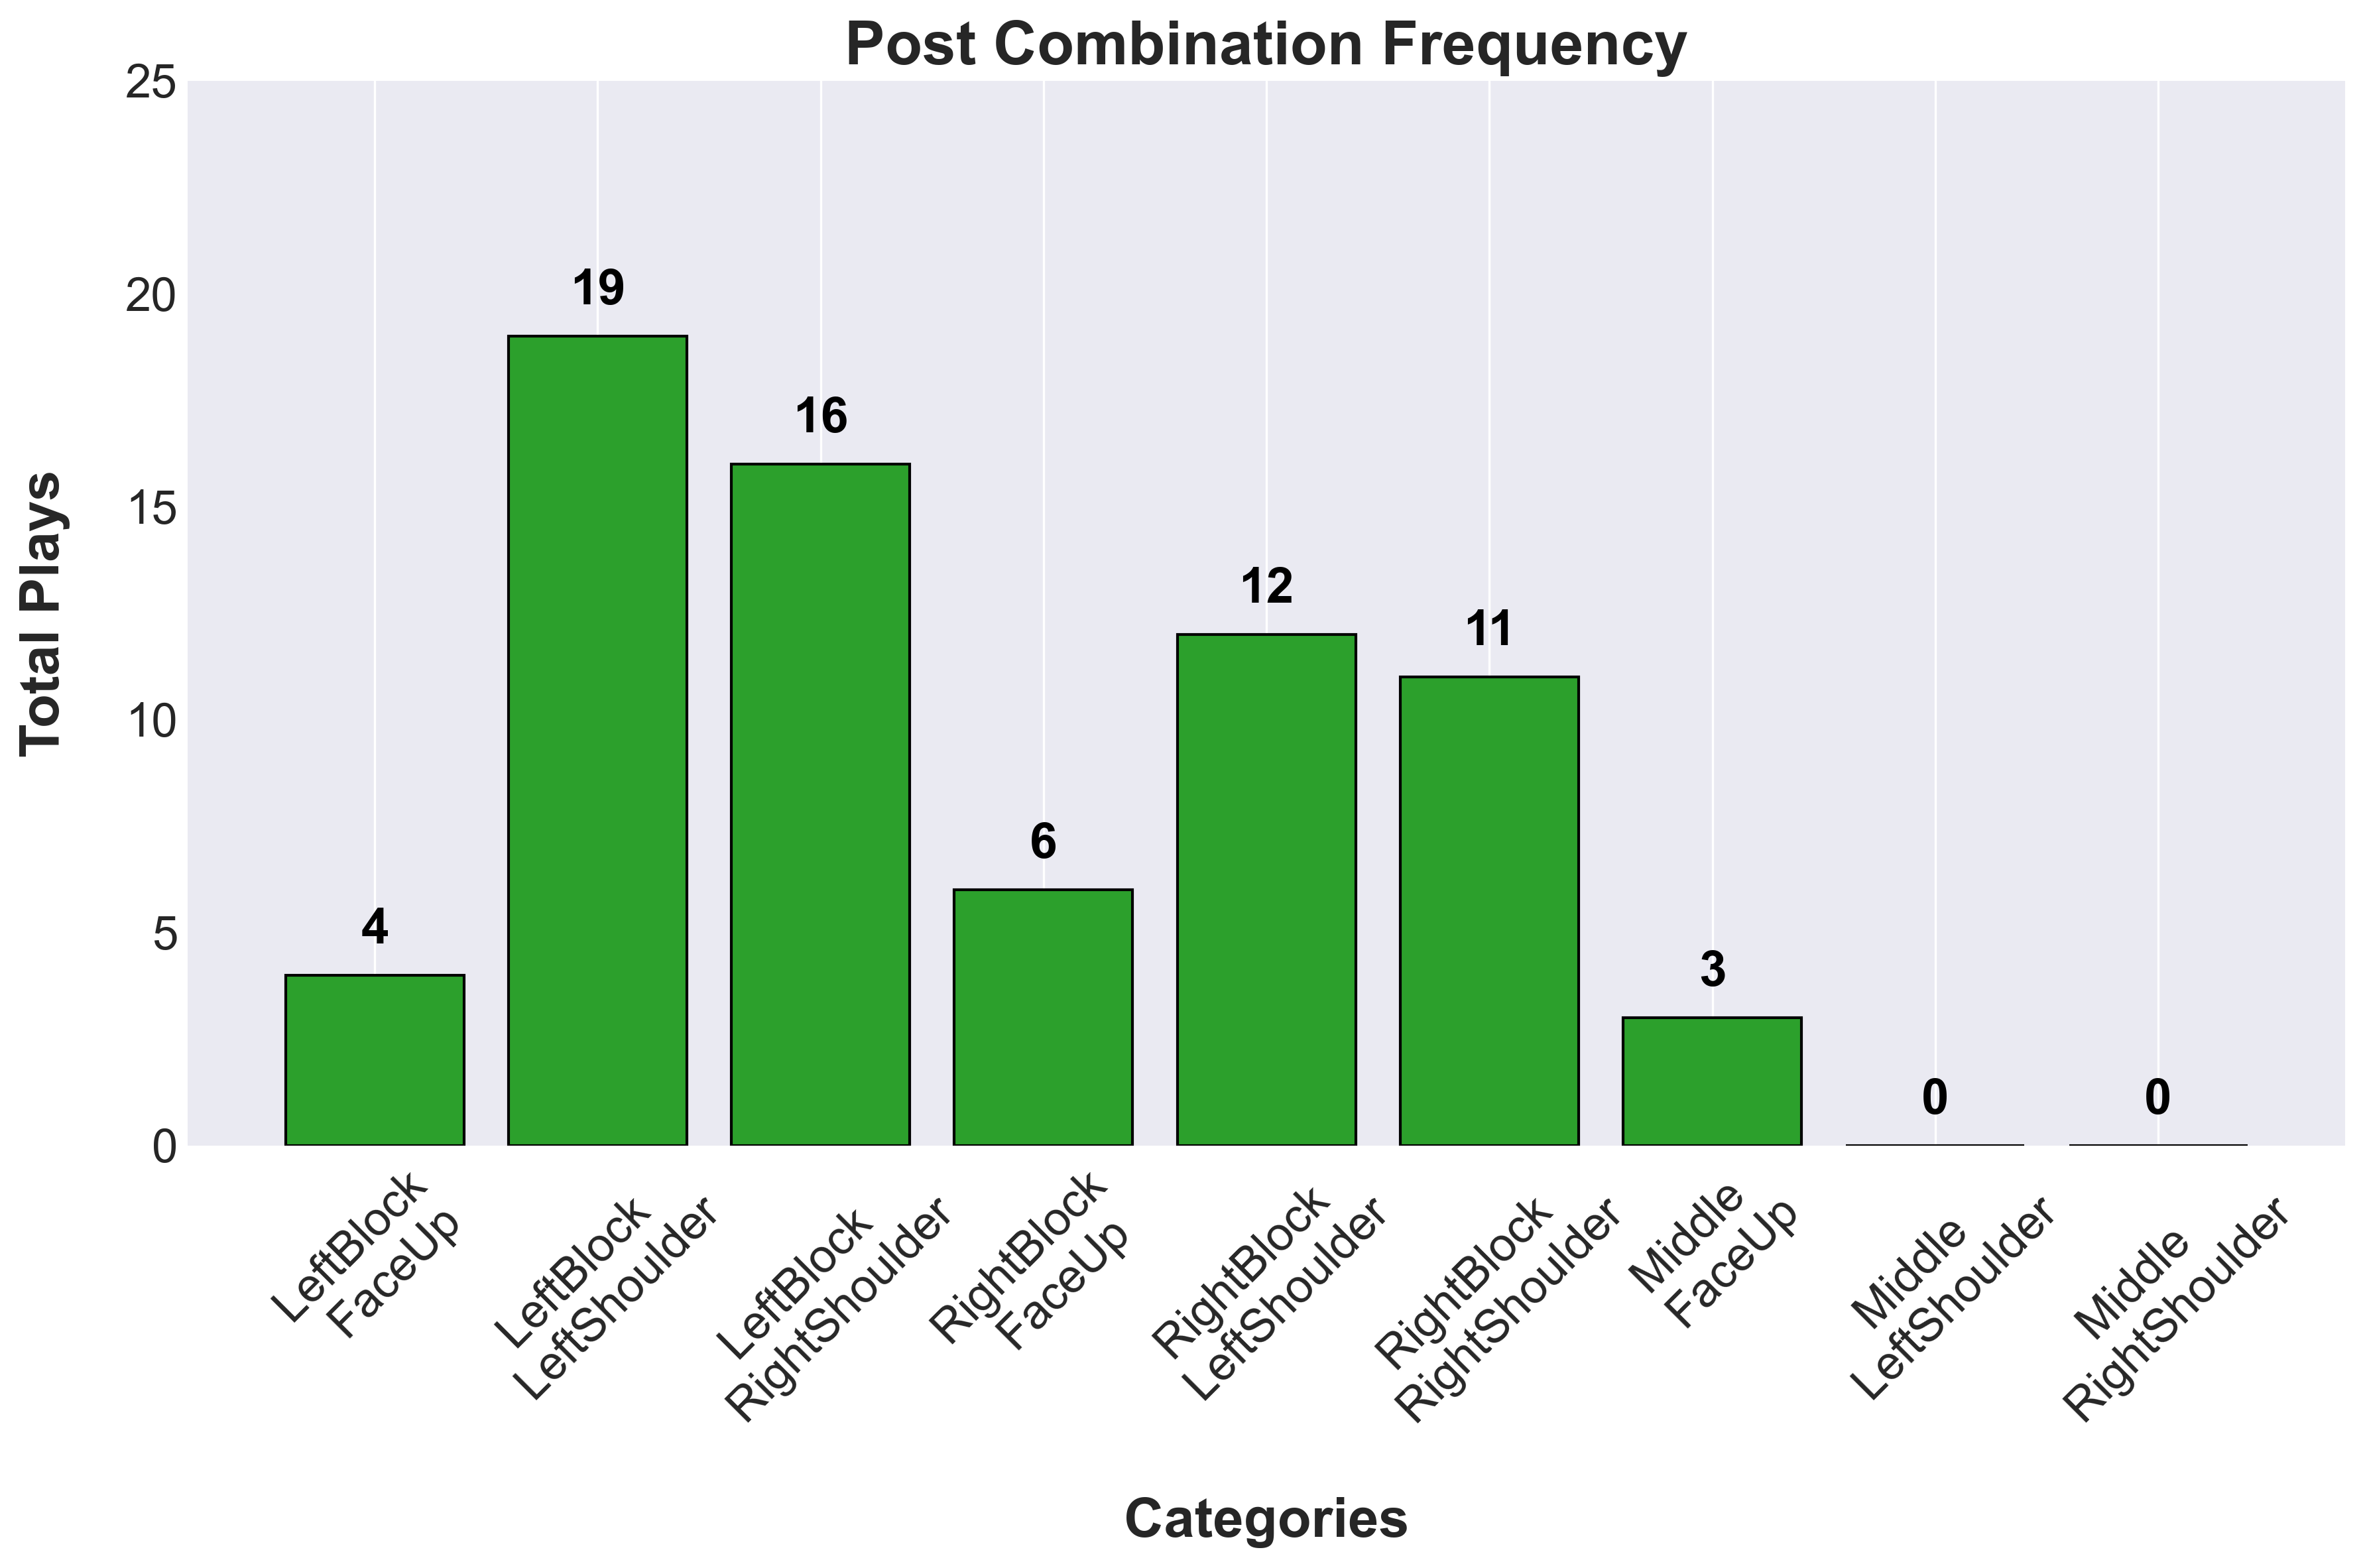
\includegraphics[width=\textwidth, height=.14\textheight]{images/Post_Combination_Freq.png} % Adjust the width of the image to fit
    \end{minipage}
\end{table}

\vspace{0em} % Add vertical space before the line (optional)
\hrule height 1pt width 1\textwidth % Adjust height and width
\vspace{1em} % Add vertical space after the line (optional)

\subsubsection{Post Passer Statistics}

\vspace{-1em} % Add vertical space before the line (optional)

% Total Post Passer Statistics
\begin{table}[H]
    \raisebox{2.5em}{ % Adjust this value to shift the tables vertically
    \begin{minipage}[t]{0.6\textwidth} % Left side (table) takes 85% of the width
        %\flushright
        \centering % Centering the title and the table
        \text{Total Post Passer Statistics} % Title above the table in bold
        \vskip .25em % Adds vertical space between title and table
        \scalebox{.85}{ % Scale the entire table down by half
            \scriptsize % Reduce the font size
            \begin{tabular}{
            >{\centering\arraybackslash}p{.75cm} 
            >{\centering\arraybackslash}p{.5cm} 
            >{\centering\arraybackslash}p{.5cm} 
            >{\centering\arraybackslash}p{.5cm}
            >{\centering\arraybackslash}p{.5cm} 
            >{\centering\arraybackslash}p{.5cm} 
            >{\centering\arraybackslash}p{.5cm} 
            >{\centering\arraybackslash}p{.5cm}
            >{\centering\arraybackslash}p{.5cm} 
            >{\centering\arraybackslash}p{.5cm}
            >{\centering\arraybackslash}p{.5cm} 
            >{\centering\arraybackslash}p{.5cm}}% Adjust column widths
            \toprule
            \textbf{Plays} &
            \textbf{3PA} &
            \textbf{3PM} &
            \textbf{3P\%} & 
            \textbf{2PA} & 
            \textbf{2PM} & 
            \textbf{2P\%} & 
            \textbf{MiA} & 
            \textbf{MiM} &
            \textbf{Mi\%} &
            \textbf{TO} &
            \textbf{Foul} \\
            \midrule
            
                
            
                
                    1 & 0 & 0 &
                    - & 
                    1 & 1 &
                    100.0 &
                    0 & 0 &
                    - &
                    0 & 0 \\
                
            
                
            
                
            
                
            
                
            
                
            
                
            
                
            
                
            
                
            
                
            
                
            
                
            
                
            
                
            
                
            
                
            
                
            
                
            
                
            
                
            
                
            


            \bottomrule
            \end{tabular}
        }
    \end{minipage}
    }
    \hfill % This adds some flexible space between the table and the image
    \begin{minipage}[c]{0.35\textwidth} % Right side (image) takes 10% of the width
        \flushright
        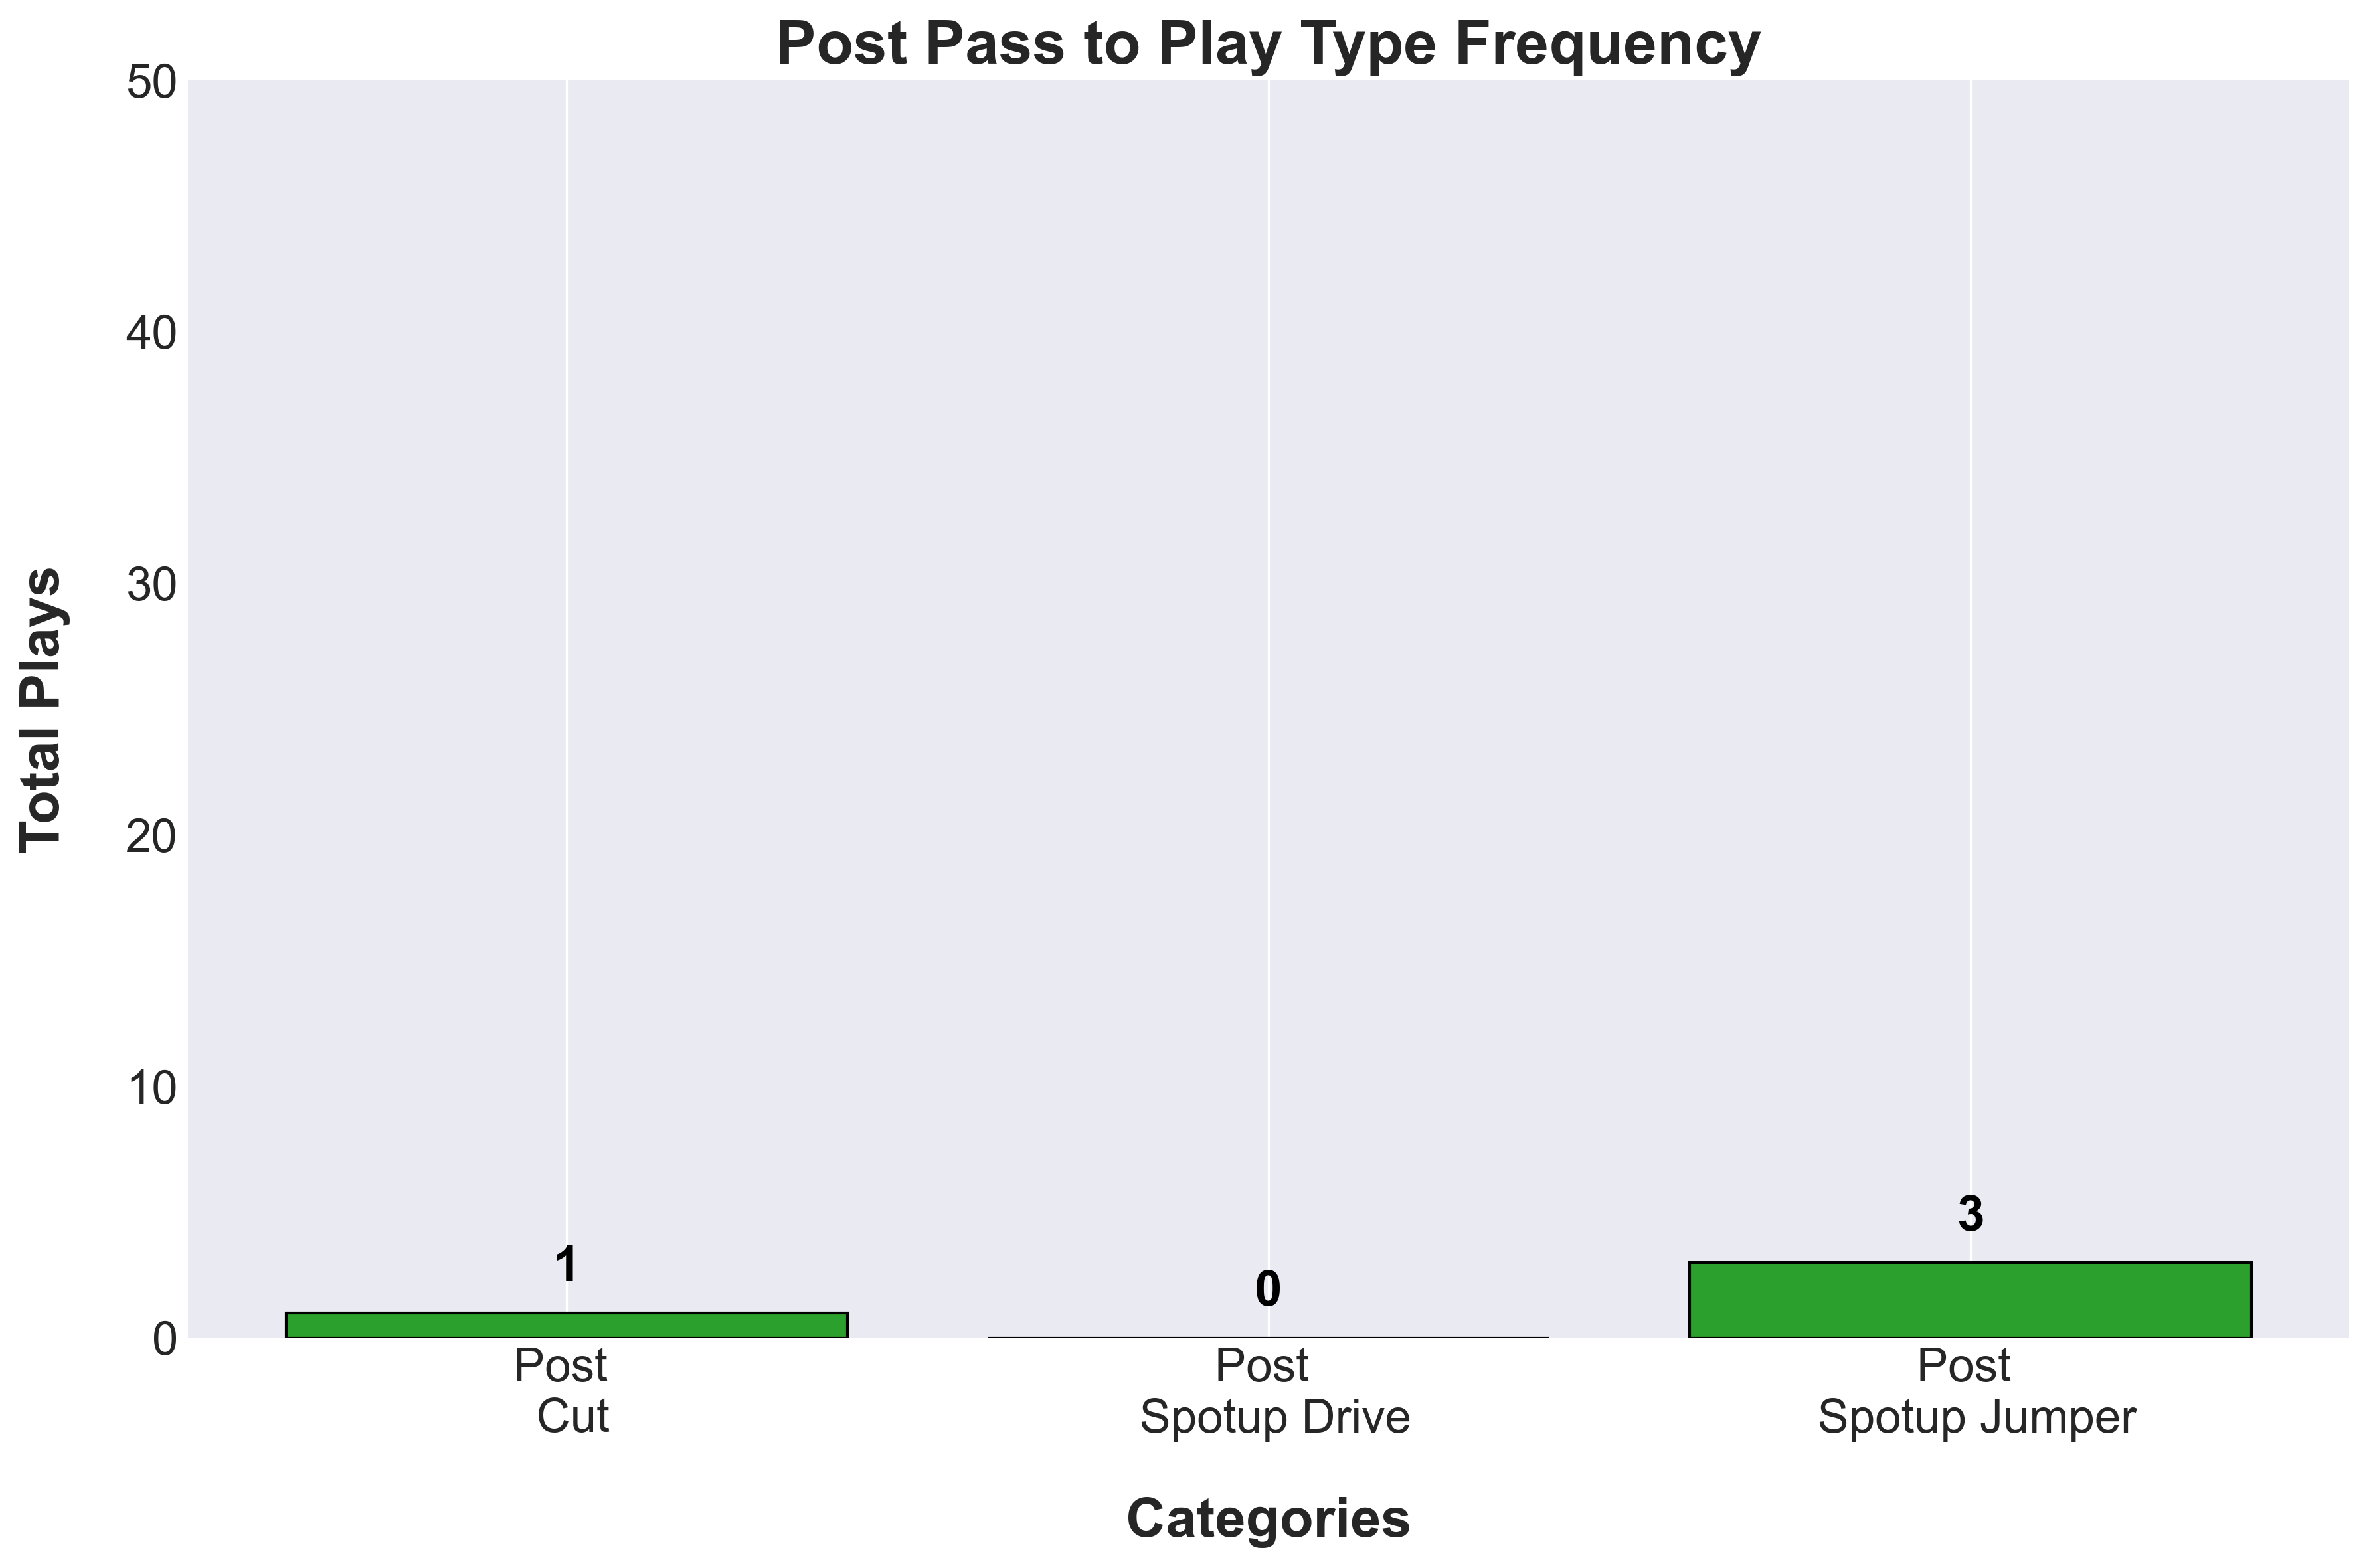
\includegraphics[width=\textwidth, height=.14\textheight]{images/Post_PassPlayType_Freq.png} % Adjust the width of the image to fit
    \end{minipage}
\end{table}

\vspace{-1em} % Add vertical space before the line (optional)
\vspace{1em} % Add vertical space after the line (optional)

% Post -> Cut Secondary Player Stats
\begin{table}[H]
    \raisebox{3em}{ % Adjust this value to shift the tables vertically
    \begin{minipage}[t]{0.6\textwidth} % Left side (table) takes 85% of the width
        \flushleft
        \centering % Centering the title and the table
        \text{Post - Cut Player Statistics} % Title above the table in bold
        \vskip .25em % Adds vertical space between title and table
        \scalebox{.55}{ % Scale the entire table down by half
            \renewcommand{\arraystretch}{1.4} % Adjust the number to increase or decrease row spacing
            \begin{tabular}{
            >{\centering\arraybackslash}p{3cm} 
            >{\centering\arraybackslash}p{.75cm} 
            >{\centering\arraybackslash}p{.75cm} 
            >{\centering\arraybackslash}p{.75cm} 
            >{\centering\arraybackslash}p{.75cm}
            >{\centering\arraybackslash}p{.75cm} 
            >{\centering\arraybackslash}p{.75cm} 
            >{\centering\arraybackslash}p{.75cm} 
            >{\centering\arraybackslash}p{.75cm} 
            >{\centering\arraybackslash}p{.75cm}}% Adjust column widths
            \toprule
            {\scriptsize \textbf{Player}} &
            {\scriptsize \textbf{Plays}} &
            {\scriptsize \textbf{2PA}} & 
            {\scriptsize \textbf{2PM}} & 
            {\scriptsize \textbf{2P\%}} & 
            {\scriptsize \textbf{MiA}} & 
            {\scriptsize \textbf{MiM}} &
            {\scriptsize \textbf{Mi\%}} &
            {\scriptsize \textbf{TO}} &
            {\scriptsize \textbf{Foul}} \\
            \midrule
            
                
            
                
            
                
                    
                        Keegan Ocorr & 
                        1 & 
                        1 & 
                        1 & 
                        100.0 & 
                        0 & 
                        0 & 
                        - & 
                        0 & 
                        0 \\
                    
                
            
                
            
                
            
                
            
                
            
                
            
                
            
                
            
                
            
                
            
                
            
                
            
                
            
                
            
                
            
                
            
                
            
                
            
                
            
                
            
                
            

            \bottomrule
        \end{tabular}
        } % End of \scalebox
    \end{minipage}
    } % End of raisebox, closing the adjustment
    \hfill % This adds some flexible space between the table and the image
    \begin{minipage}[c]{0.35\textwidth} % Right side (image) takes 10% of the width
        \flushright
        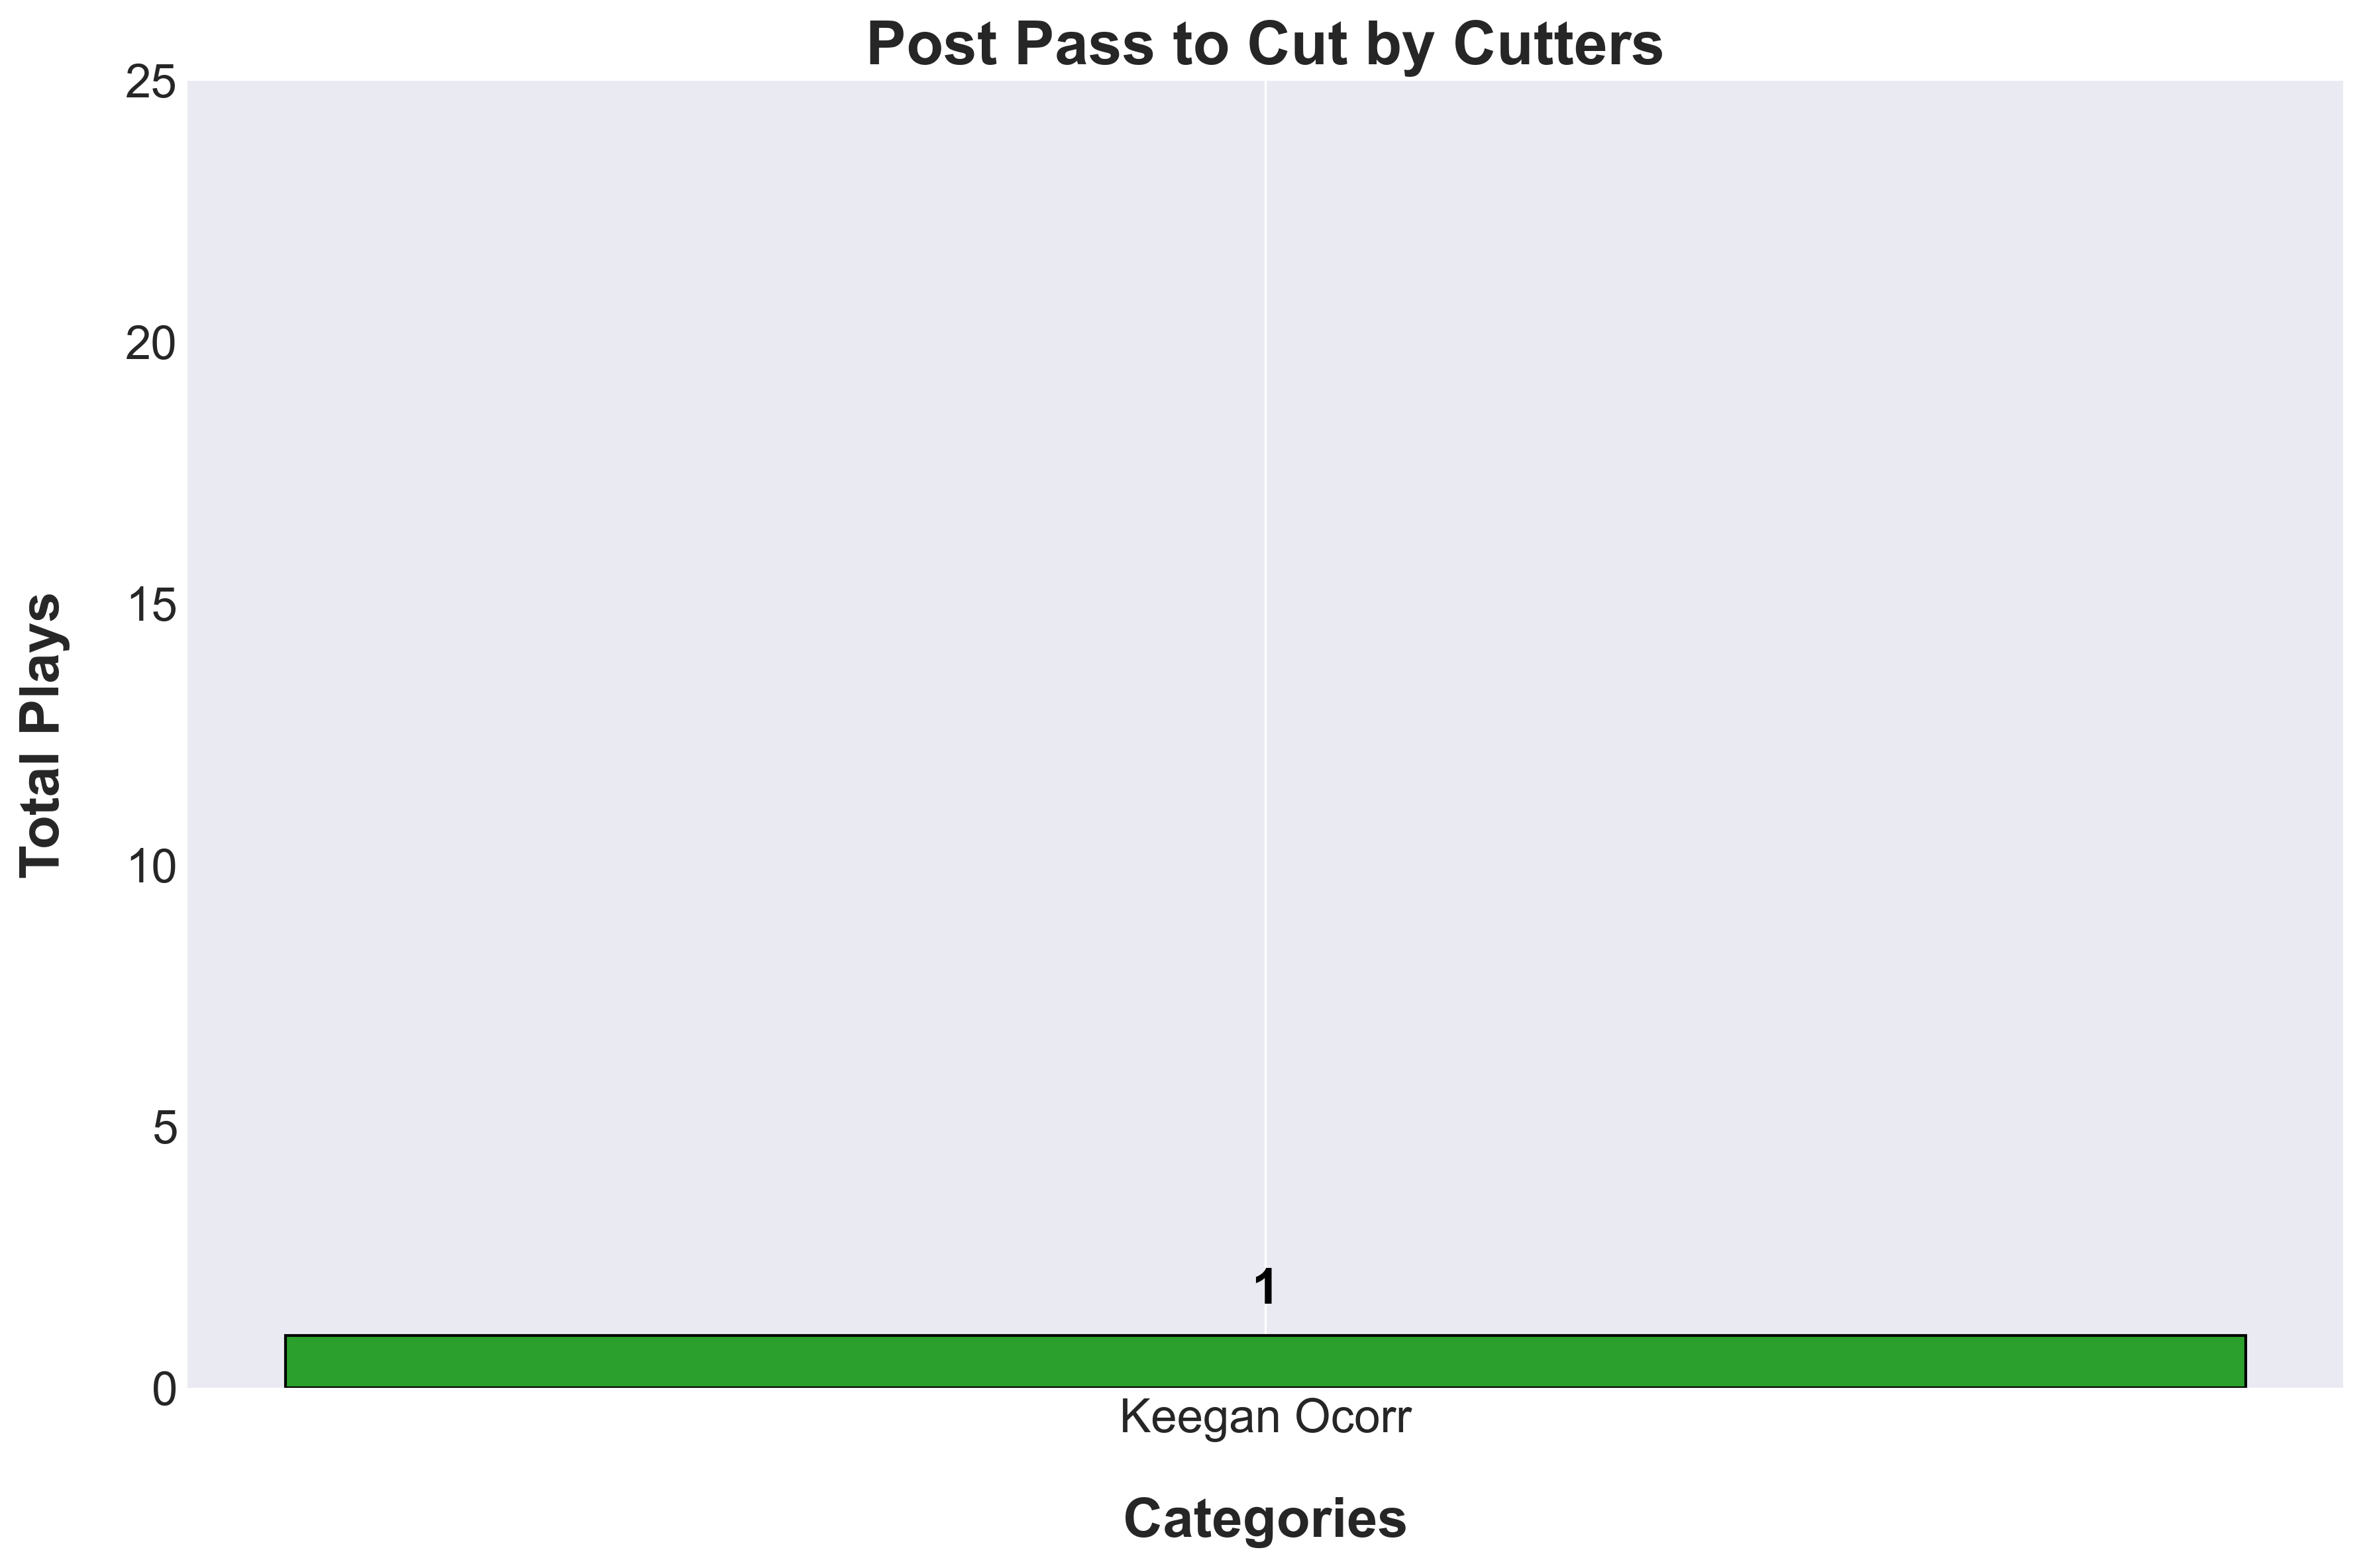
\includegraphics[width=\textwidth, height=.14\textheight]{images/Post_PassCutsPlayer_Freq.png} % Adjust the width of the image to fit
    \end{minipage}
\end{table}

\vspace{-1em} % Add vertical space before the line (optional)
\vspace{-1em} % Add vertical space after the line (optional)

% Post -> Spot Up Drives Secondary Player Stats
\begin{table}[H]
    \raisebox{3em}{ % Adjust this value to shift the tables vertically
    \begin{minipage}[t]{0.6\textwidth} % Left side (table) takes 85% of the width
        \flushleft
        \centering % Centering the title and the table
        \text{Post - Spot Up Drives Player Statistics} % Title above the table in bold
        \vskip .25em % Adds vertical space between title and table
        \scalebox{.55}{ % Scale the entire table down by half
            \renewcommand{\arraystretch}{1.4} % Adjust the number to increase or decrease row spacing
            \begin{tabular}{
            >{\centering\arraybackslash}p{3cm} 
            >{\centering\arraybackslash}p{.75cm} 
            >{\centering\arraybackslash}p{.75cm} 
            >{\centering\arraybackslash}p{.75cm} 
            >{\centering\arraybackslash}p{.75cm}
            >{\centering\arraybackslash}p{.75cm} 
            >{\centering\arraybackslash}p{.75cm} 
            >{\centering\arraybackslash}p{.75cm} 
            >{\centering\arraybackslash}p{.75cm}
            >{\centering\arraybackslash}p{.75cm} 
            >{\centering\arraybackslash}p{.75cm}
            >{\centering\arraybackslash}p{.75cm} 
            >{\centering\arraybackslash}p{.75cm}}% Adjust column widths
            \toprule
            {\scriptsize \textbf{Player}} &
            {\scriptsize \textbf{Plays}} &
            {\scriptsize \textbf{3PA}} &
            {\scriptsize \textbf{3PM}} &
            {\scriptsize \textbf{3P\%}} & 
            {\scriptsize \textbf{2PA}} & 
            {\scriptsize \textbf{2PM}} & 
            {\scriptsize \textbf{2P\%}} & 
            {\scriptsize \textbf{MiA}} & 
            {\scriptsize \textbf{MiM}} &
            {\scriptsize \textbf{Mi\%}} &
            {\scriptsize \textbf{TO}} &
            {\scriptsize \textbf{Foul}} \\
            \midrule
            
                
            
                
            
                
            
                
                    
                
            
                
            
                
            
                
            
                
            
                
            
                
            
                
            
                
            
                
            
                
            
                
            
                
            
                
            
                
            
                
            
                
            
                
            
                
            
                
            

            \bottomrule
        \end{tabular}
        } % End of \scalebox
    \end{minipage}
    } % End of raisebox, closing the adjustment
    \hfill % This adds some flexible space between the table and the image
    \begin{minipage}[c]{0.35\textwidth} % Right side (image) takes 10% of the width
        \flushright
        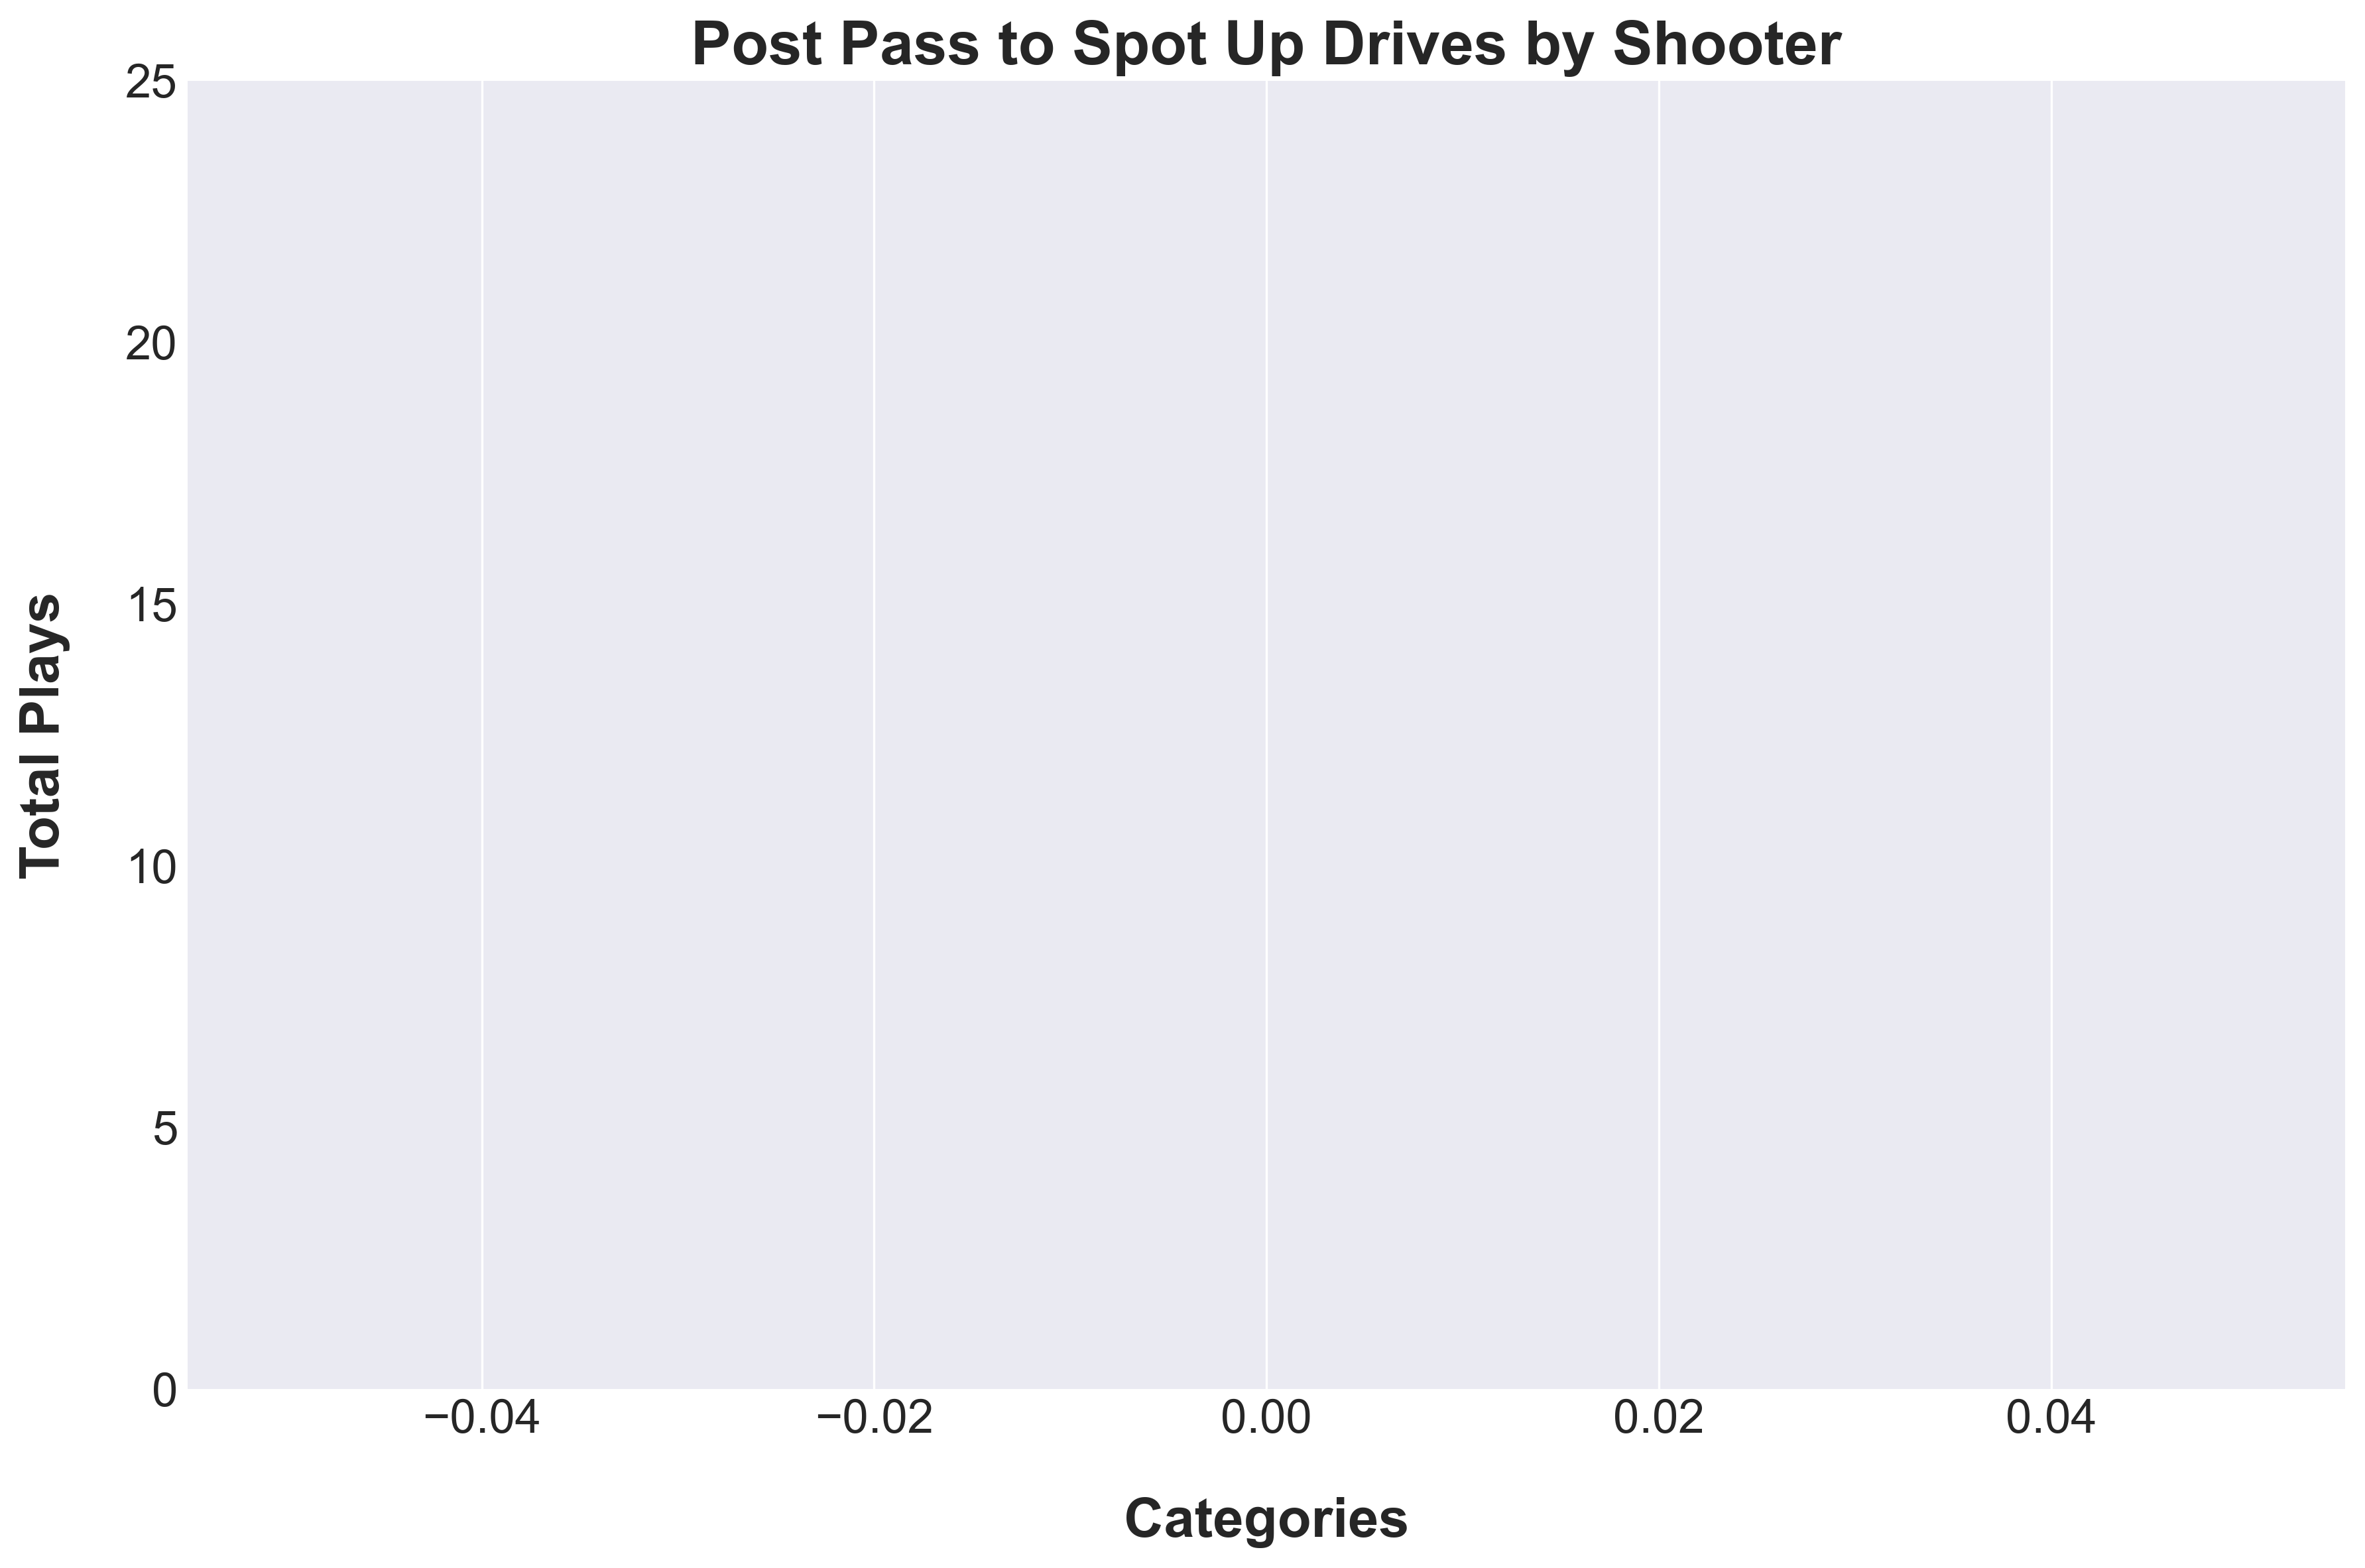
\includegraphics[width=\textwidth, height=.14\textheight]{images/Post_PassDrivesPlayer_Freq.png} % Adjust the width of the image to fit
    \end{minipage}
\end{table}

\vspace{-1em} % Add vertical space before the line (optional)
\vspace{-1em} % Add vertical space after the line (optional)

% Post -> Spot Up Jumpers Secondary Player Stats
\begin{table}[H]
    \raisebox{3em}{ % Adjust this value to shift the tables vertically
    \begin{minipage}[t]{0.6\textwidth} % Left side (table) takes 85% of the width
        \flushleft
        \centering % Centering the title and the table
        \text{Post - Spot Up Jumpers Player Statistics} % Title above the table in bold
        \vskip .25em % Adds vertical space between title and table
        \scalebox{.55}{ % Scale the entire table down by half
            \renewcommand{\arraystretch}{1.4} % Adjust the number to increase or decrease row spacing
            \begin{tabular}{
            >{\centering\arraybackslash}p{3cm} 
            >{\centering\arraybackslash}p{.75cm} 
            >{\centering\arraybackslash}p{.75cm} 
            >{\centering\arraybackslash}p{.75cm} 
            >{\centering\arraybackslash}p{.75cm} 
            >{\centering\arraybackslash}p{.75cm}
            >{\centering\arraybackslash}p{.75cm} 
            >{\centering\arraybackslash}p{.75cm}
            >{\centering\arraybackslash}p{.75cm} 
            >{\centering\arraybackslash}p{.75cm}}% Adjust column widths
            \toprule
            {\scriptsize \textbf{Player}} &
            {\scriptsize \textbf{Plays}} &
            {\scriptsize \textbf{3PA}} &
            {\scriptsize \textbf{3PM}} &
            {\scriptsize \textbf{3P\%}} & 
            {\scriptsize \textbf{MiA}} & 
            {\scriptsize \textbf{MiM}} &
            {\scriptsize \textbf{Mi\%}} &
            {\scriptsize \textbf{TO}} &
            {\scriptsize \textbf{Foul}} \\
            \midrule
            
                
            
                
            
                
            
                
            
                
                    
                
            
                
            
                
            
                
            
                
            
                
            
                
            
                
            
                
            
                
            
                
            
                
            
                
            
                
            
                
            
                
            
                
            
                
            
                
            

            \bottomrule
        \end{tabular}
        } % End of \scalebox
    \end{minipage}
    } % End of raisebox, closing the adjustment
    \hfill % This adds some flexible space between the table and the image
    \begin{minipage}[c]{0.35\textwidth} % Right side (image) takes 10% of the width
        \flushright
        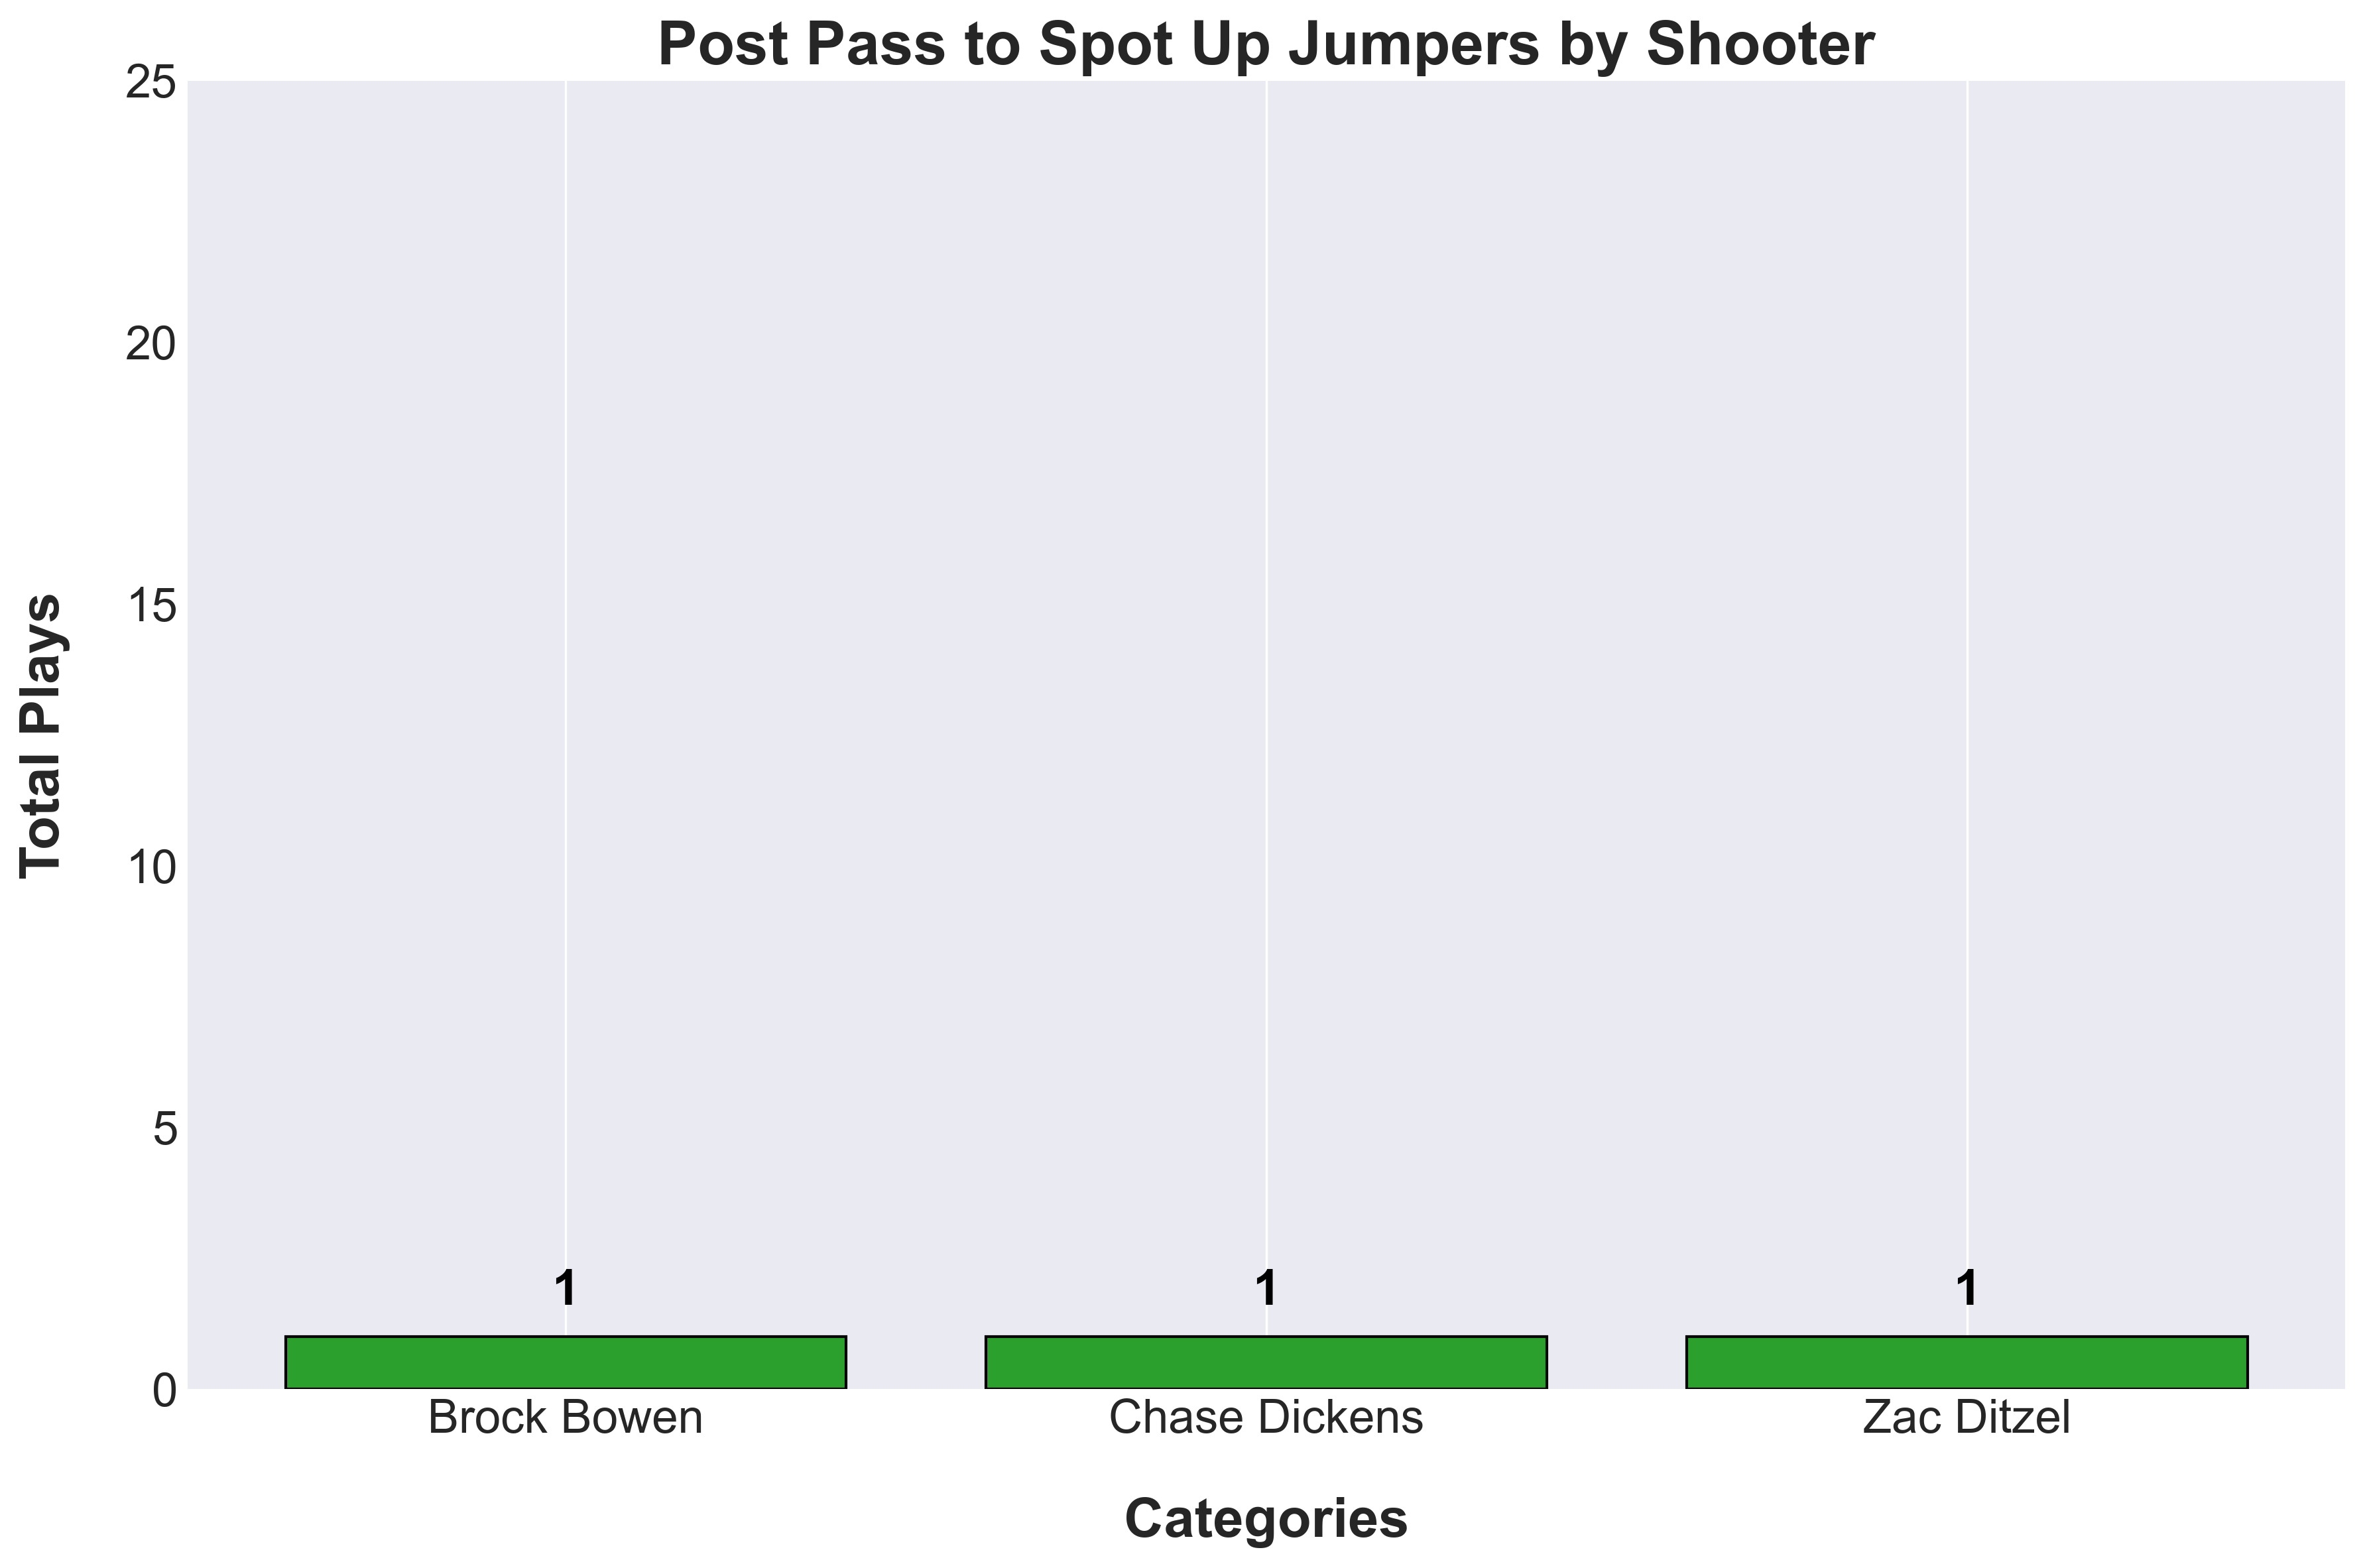
\includegraphics[width=\textwidth, height=.14\textheight]{images/Post_PassShotsPlayer_Freq.png} % Adjust the width of the image to fit
    \end{minipage}
\end{table}

\vspace{-1em} % Add vertical space before the line (optional)
\hrule height 1pt width 1\textwidth % Adjust height and width
\vspace{1em} % Add vertical space after the line (optional)

\clearpage




% ----------------------
% Rollman Visuals and Insights Section
% ----------------------
\subsection{Rollman}\

\vspace{0.25em} % Add vertical space before the line (optional)
\textbf{Key Notes on Rollman Tendencies}
\vspace{0.5em} % Add space between the title and the itemized list

\begin{itemize}
    \item Rollman Plays make up x\% of players offensive load
    \vspace{0.3em} % Add space between the title and the itemized list
    \item Player is more efficient shooting over his left shoulder and get shots off of the left block x\% of the time which is much higher than the middle and right block.
\end{itemize}

\vspace{1em} % Add vertical space after the line (optional)
\hrule height 1pt width 1\textwidth % Adjust height and width
\vspace{0em} % Add vertical space after the line (optional)

\subsubsection{Rollman General Scorer Stats}
% All Rollman Statistics Table w/ room for insights
\begin{table}[H]
    \centering
    \begin{minipage}[t]{0.6\textwidth} % Left side (table) takes 85% of the width
        %\flushright
        \centering % Centering the title and the table
        \text{Total Rollman Shot Statistics} % Title above the table in bold
        \vskip .25em % Adds vertical space between title and table
        \scalebox{.85}{ % Scale the entire table down by half
            \scriptsize % Reduce the font size
            \begin{tabular}{
            >{\centering\arraybackslash}p{.75cm} 
            >{\centering\arraybackslash}p{.5cm} 
            >{\centering\arraybackslash}p{.5cm} 
            >{\centering\arraybackslash}p{.5cm}
            >{\centering\arraybackslash}p{.5cm} 
            >{\centering\arraybackslash}p{.5cm} 
            >{\centering\arraybackslash}p{.5cm} 
            >{\centering\arraybackslash}p{.5cm}
            >{\centering\arraybackslash}p{.5cm} 
            >{\centering\arraybackslash}p{.5cm}
            >{\centering\arraybackslash}p{.5cm} 
            >{\centering\arraybackslash}p{.5cm}}% Adjust column widths
            \toprule
            \textbf{Plays} &
            \textbf{3PA} &
            \textbf{3PM} &
            \textbf{3P\%} & 
            \textbf{2PA} & 
            \textbf{2PM} & 
            \textbf{2P\%} & 
            \textbf{MiA} & 
            \textbf{MiM} &
            \textbf{Mi\%} &
            \textbf{TO} &
            \textbf{Foul} \\
            \midrule
            
                
            
                
            
                
            
                
            
                
            
                
            
                
            
                
            
                
            
                
            
                
            
                
            
                
            
                
            
                
            
                
            
            \bottomrule
            \end{tabular}
        }
    \end{minipage}
\end{table}

\vspace{0em} % Add vertical space before the line (optional)
%\hrule height 1pt width 1\textwidth % Adjust height and width
\vspace{-1em} % Add vertical space after the line (optional)

% Rollman Stats for Slip vs Pop vs Roll 
\begin{table}[H]
    \raisebox{3em}{ % Adjust this value to shift the tables vertically
    \begin{minipage}[t]{0.6\textwidth} % Left side (table) takes 85% of the width
        \flushleft
        \centering % Centering the title and the table
        \text{Rollman Play Type Statistics} % Title above the table in bold
        \vskip .25em % Adds vertical space between title and table
        \scalebox{.6}{ % Scale the entire table down by half
            \renewcommand{\arraystretch}{1.4} % Adjust the number to increase or decrease row spacing
            \begin{tabular}{
            >{\centering\arraybackslash}p{1.75cm} 
            >{\centering\arraybackslash}p{.75cm} 
            >{\centering\arraybackslash}p{.75cm} 
            >{\centering\arraybackslash}p{.75cm} 
            >{\centering\arraybackslash}p{.75cm}
            >{\centering\arraybackslash}p{.75cm} 
            >{\centering\arraybackslash}p{.75cm} 
            >{\centering\arraybackslash}p{.75cm} 
            >{\centering\arraybackslash}p{.75cm}
            >{\centering\arraybackslash}p{.75cm} 
            >{\centering\arraybackslash}p{.75cm}
            >{\centering\arraybackslash}p{.75cm} 
            >{\centering\arraybackslash}p{.75cm}}% Adjust column widths
            \toprule
            {\scriptsize \textbf{PlayType}} &
            {\scriptsize \textbf{Plays}} &
            {\scriptsize \textbf{3PA}} &
            {\scriptsize \textbf{3PM}} &
            {\scriptsize \textbf{3P\%}} & 
            {\scriptsize \textbf{2PA}} & 
            {\scriptsize \textbf{2PM}} & 
            {\scriptsize \textbf{2P\%}} & 
            {\scriptsize \textbf{MiA}} & 
            {\scriptsize \textbf{MiM}} &
            {\scriptsize \textbf{Mi\%}} &
            {\scriptsize \textbf{TO}} &
            {\scriptsize \textbf{Foul}} \\
            \midrule
            
                
            
                
            
                
            
                
            
                
            
                
            
                
            
                
            
                
            
                
            
                
            
                
            
                
            
                
            
                
            
                
            


            \bottomrule
        \end{tabular}
        } % End of \scalebox
    \end{minipage}
    } % End of raisebox, closing the adjustment
    \hfill % This adds some flexible space between the table and the image
    \begin{minipage}[c]{0.35\textwidth} % Right side (image) takes 10% of the width
        \flushright
        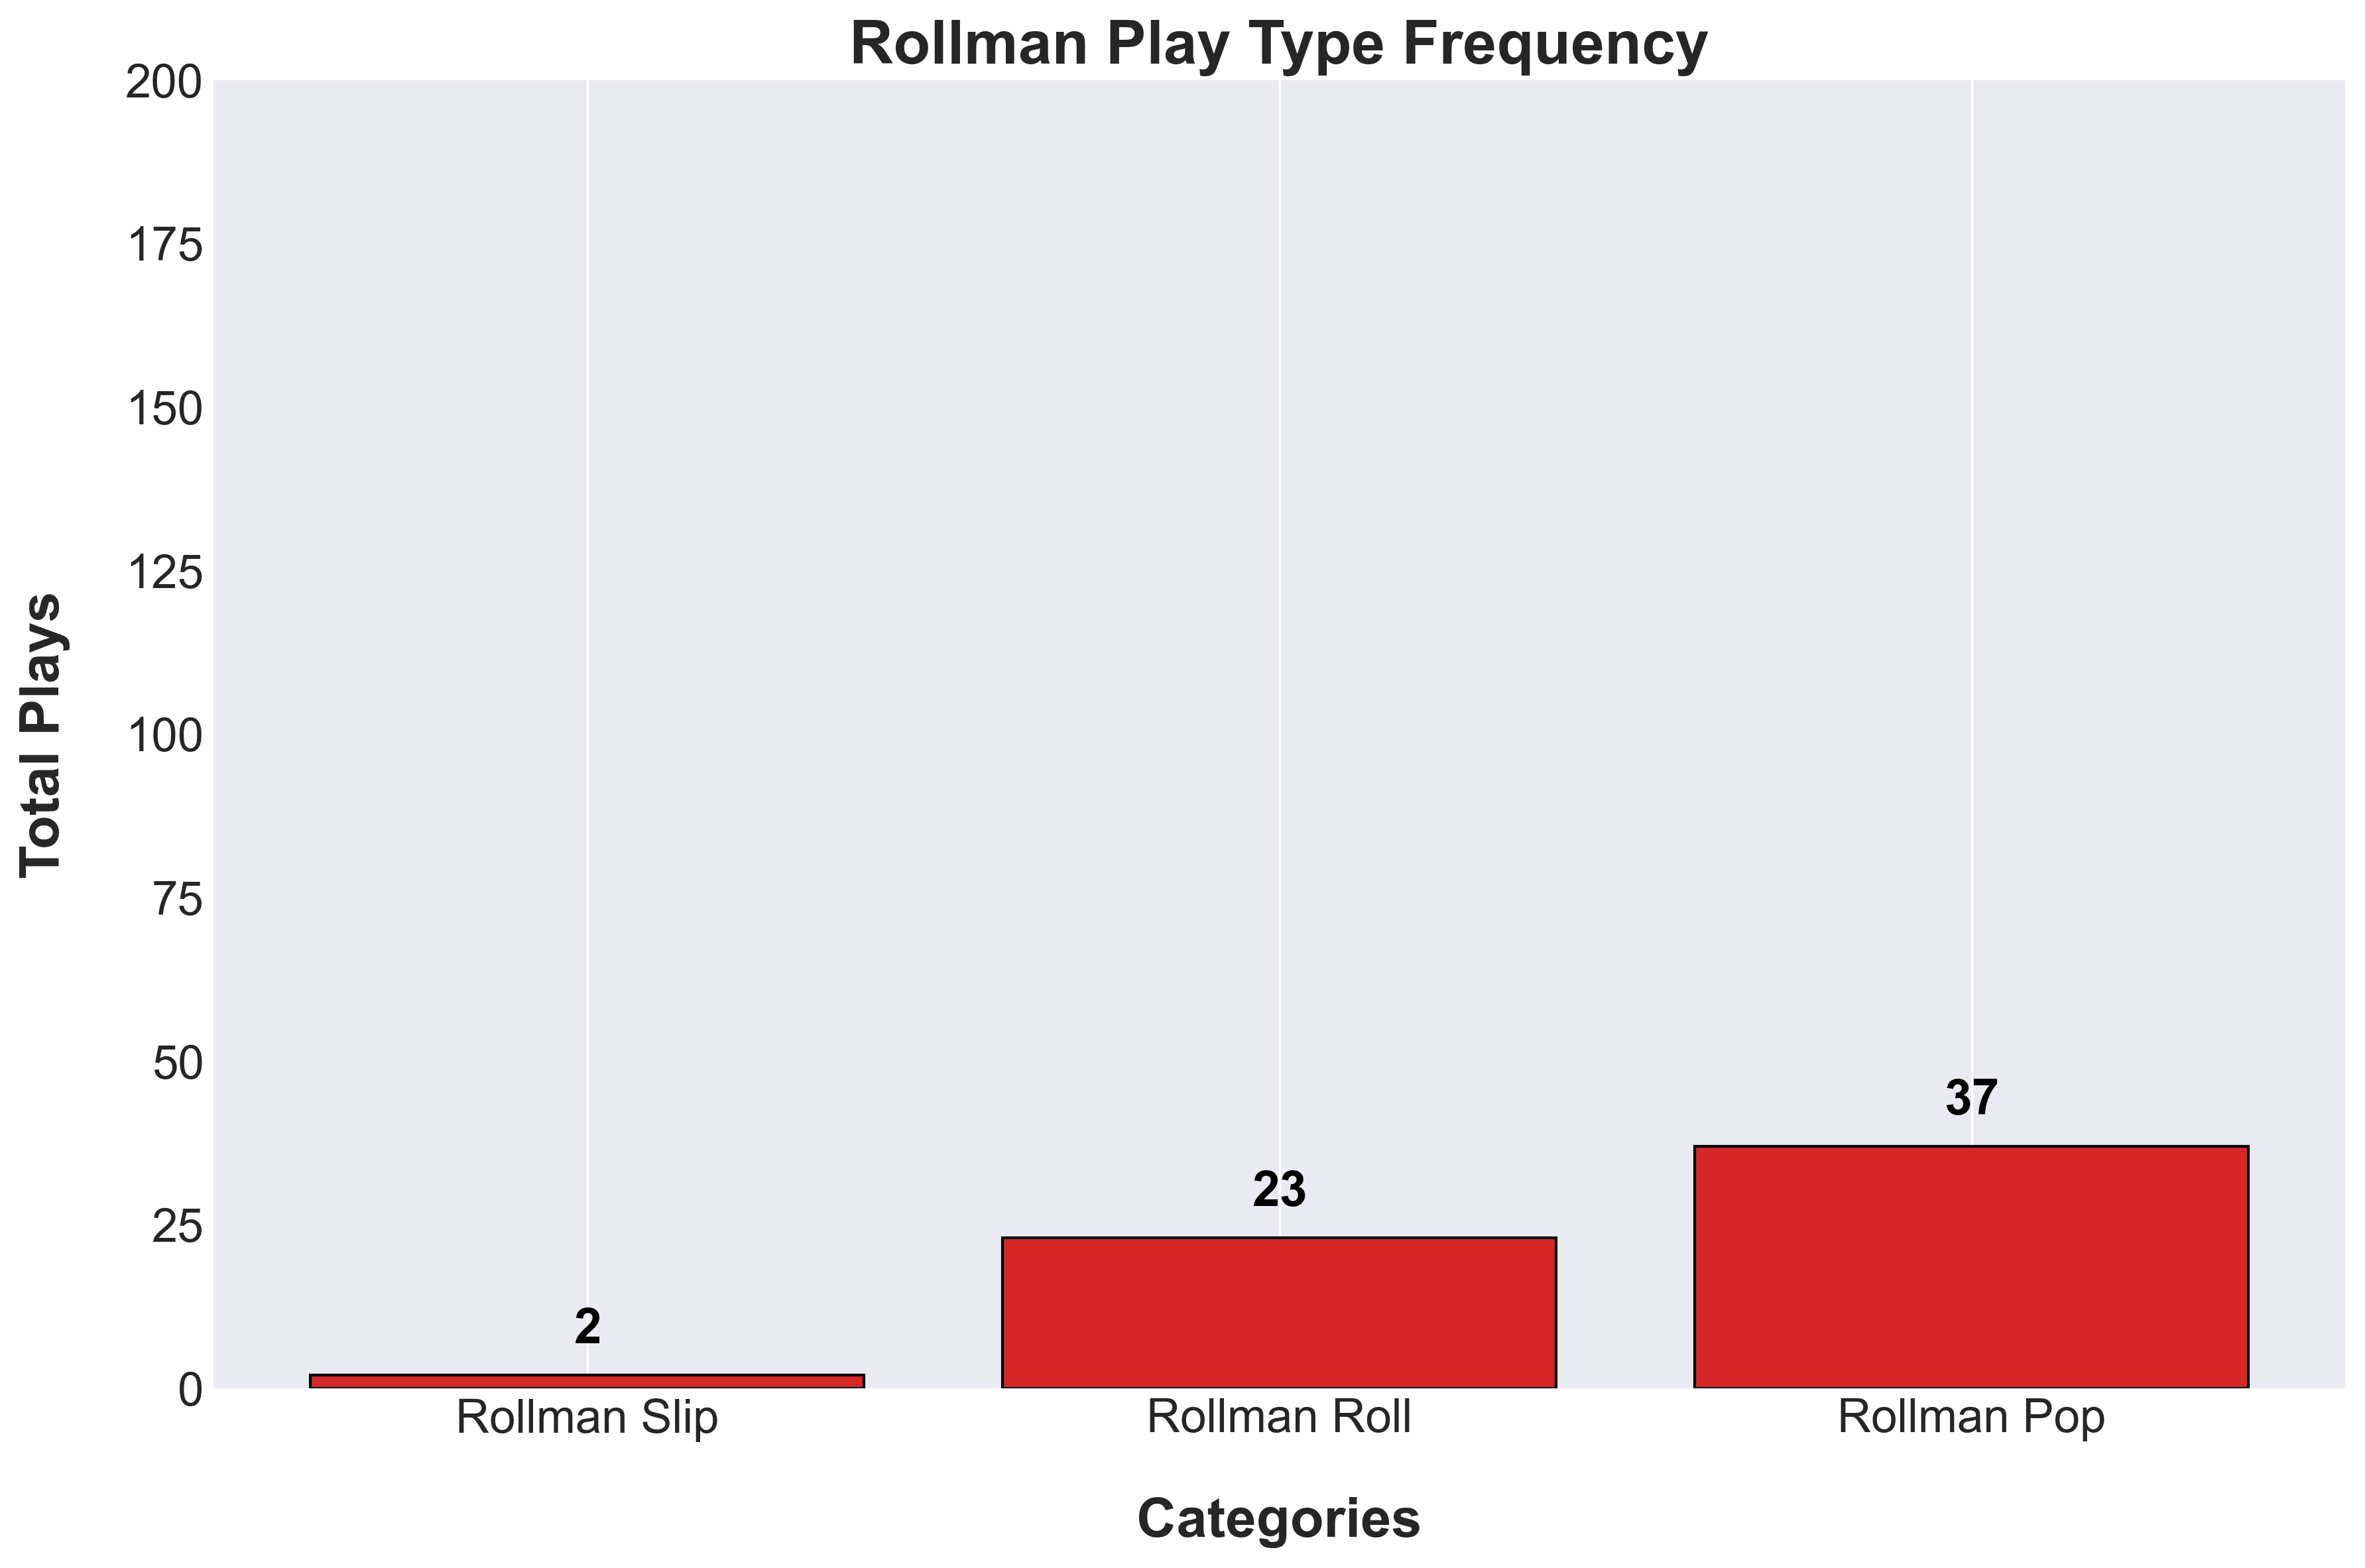
\includegraphics[width=\textwidth, height=.14\textheight]{images/Rollman_PlayType_Freq.png} % Adjust the width of the image to fit
    \end{minipage}
\end{table}

\vspace{-1em} % Add vertical space before the line (optional)
%\hrule height 1pt width 1\textwidth % Adjust height and width
\vspace{-1em} % Add vertical space after the line (optional)

% Rollman Slip Drive Direction
\begin{table}[H]
    \raisebox{3.5em}{ % Adjust this value to shift the tables vertically
    \begin{minipage}[t]{0.6\textwidth} % Left side (table) takes 85% of the width
        \flushleft
        \centering % Centering the title and the table
        \text{Rollman Slip to Drive Direction Statistics} % Title above the table in bold
        \vskip .25em % Adds vertical space between title and table
        \scalebox{.6}{ % Scale the entire table down by half
            \renewcommand{\arraystretch}{1.4} % Adjust the number to increase or decrease row spacing
            \begin{tabular}{
            >{\centering\arraybackslash}p{1.75cm} 
            >{\centering\arraybackslash}p{.75cm} 
            >{\centering\arraybackslash}p{.75cm} 
            >{\centering\arraybackslash}p{.75cm} 
            >{\centering\arraybackslash}p{.75cm}
            >{\centering\arraybackslash}p{.75cm} 
            >{\centering\arraybackslash}p{.75cm} 
            >{\centering\arraybackslash}p{.75cm} 
            >{\centering\arraybackslash}p{.75cm}
            >{\centering\arraybackslash}p{.75cm} 
            >{\centering\arraybackslash}p{.75cm}
            >{\centering\arraybackslash}p{.75cm} 
            >{\centering\arraybackslash}p{.75cm}}% Adjust column widths
            \toprule
            {\scriptsize \textbf{PlayType}} &
            {\scriptsize \textbf{Plays}} &
            {\scriptsize \textbf{3PA}} &
            {\scriptsize \textbf{3PM}} &
            {\scriptsize \textbf{3P\%}} & 
            {\scriptsize \textbf{2PA}} & 
            {\scriptsize \textbf{2PM}} & 
            {\scriptsize \textbf{2P\%}} & 
            {\scriptsize \textbf{MiA}} & 
            {\scriptsize \textbf{MiM}} &
            {\scriptsize \textbf{Mi\%}} &
            {\scriptsize \textbf{TO}} &
            {\scriptsize \textbf{Foul}} \\
            \midrule
            
                
            
                
            
                
            
                
            
                
            
                
            
                
            
                
            
                
            
                
            
                
            
                
            
                
            
                
            
                
            
                
            


            \bottomrule
        \end{tabular}
        } % End of \scalebox
    \end{minipage}
    } % End of raisebox, closing the adjustment
    \hfill
    \begin{minipage}[c]{0.35\textwidth} % Right side (image) takes 10% of the width
        \flushright
        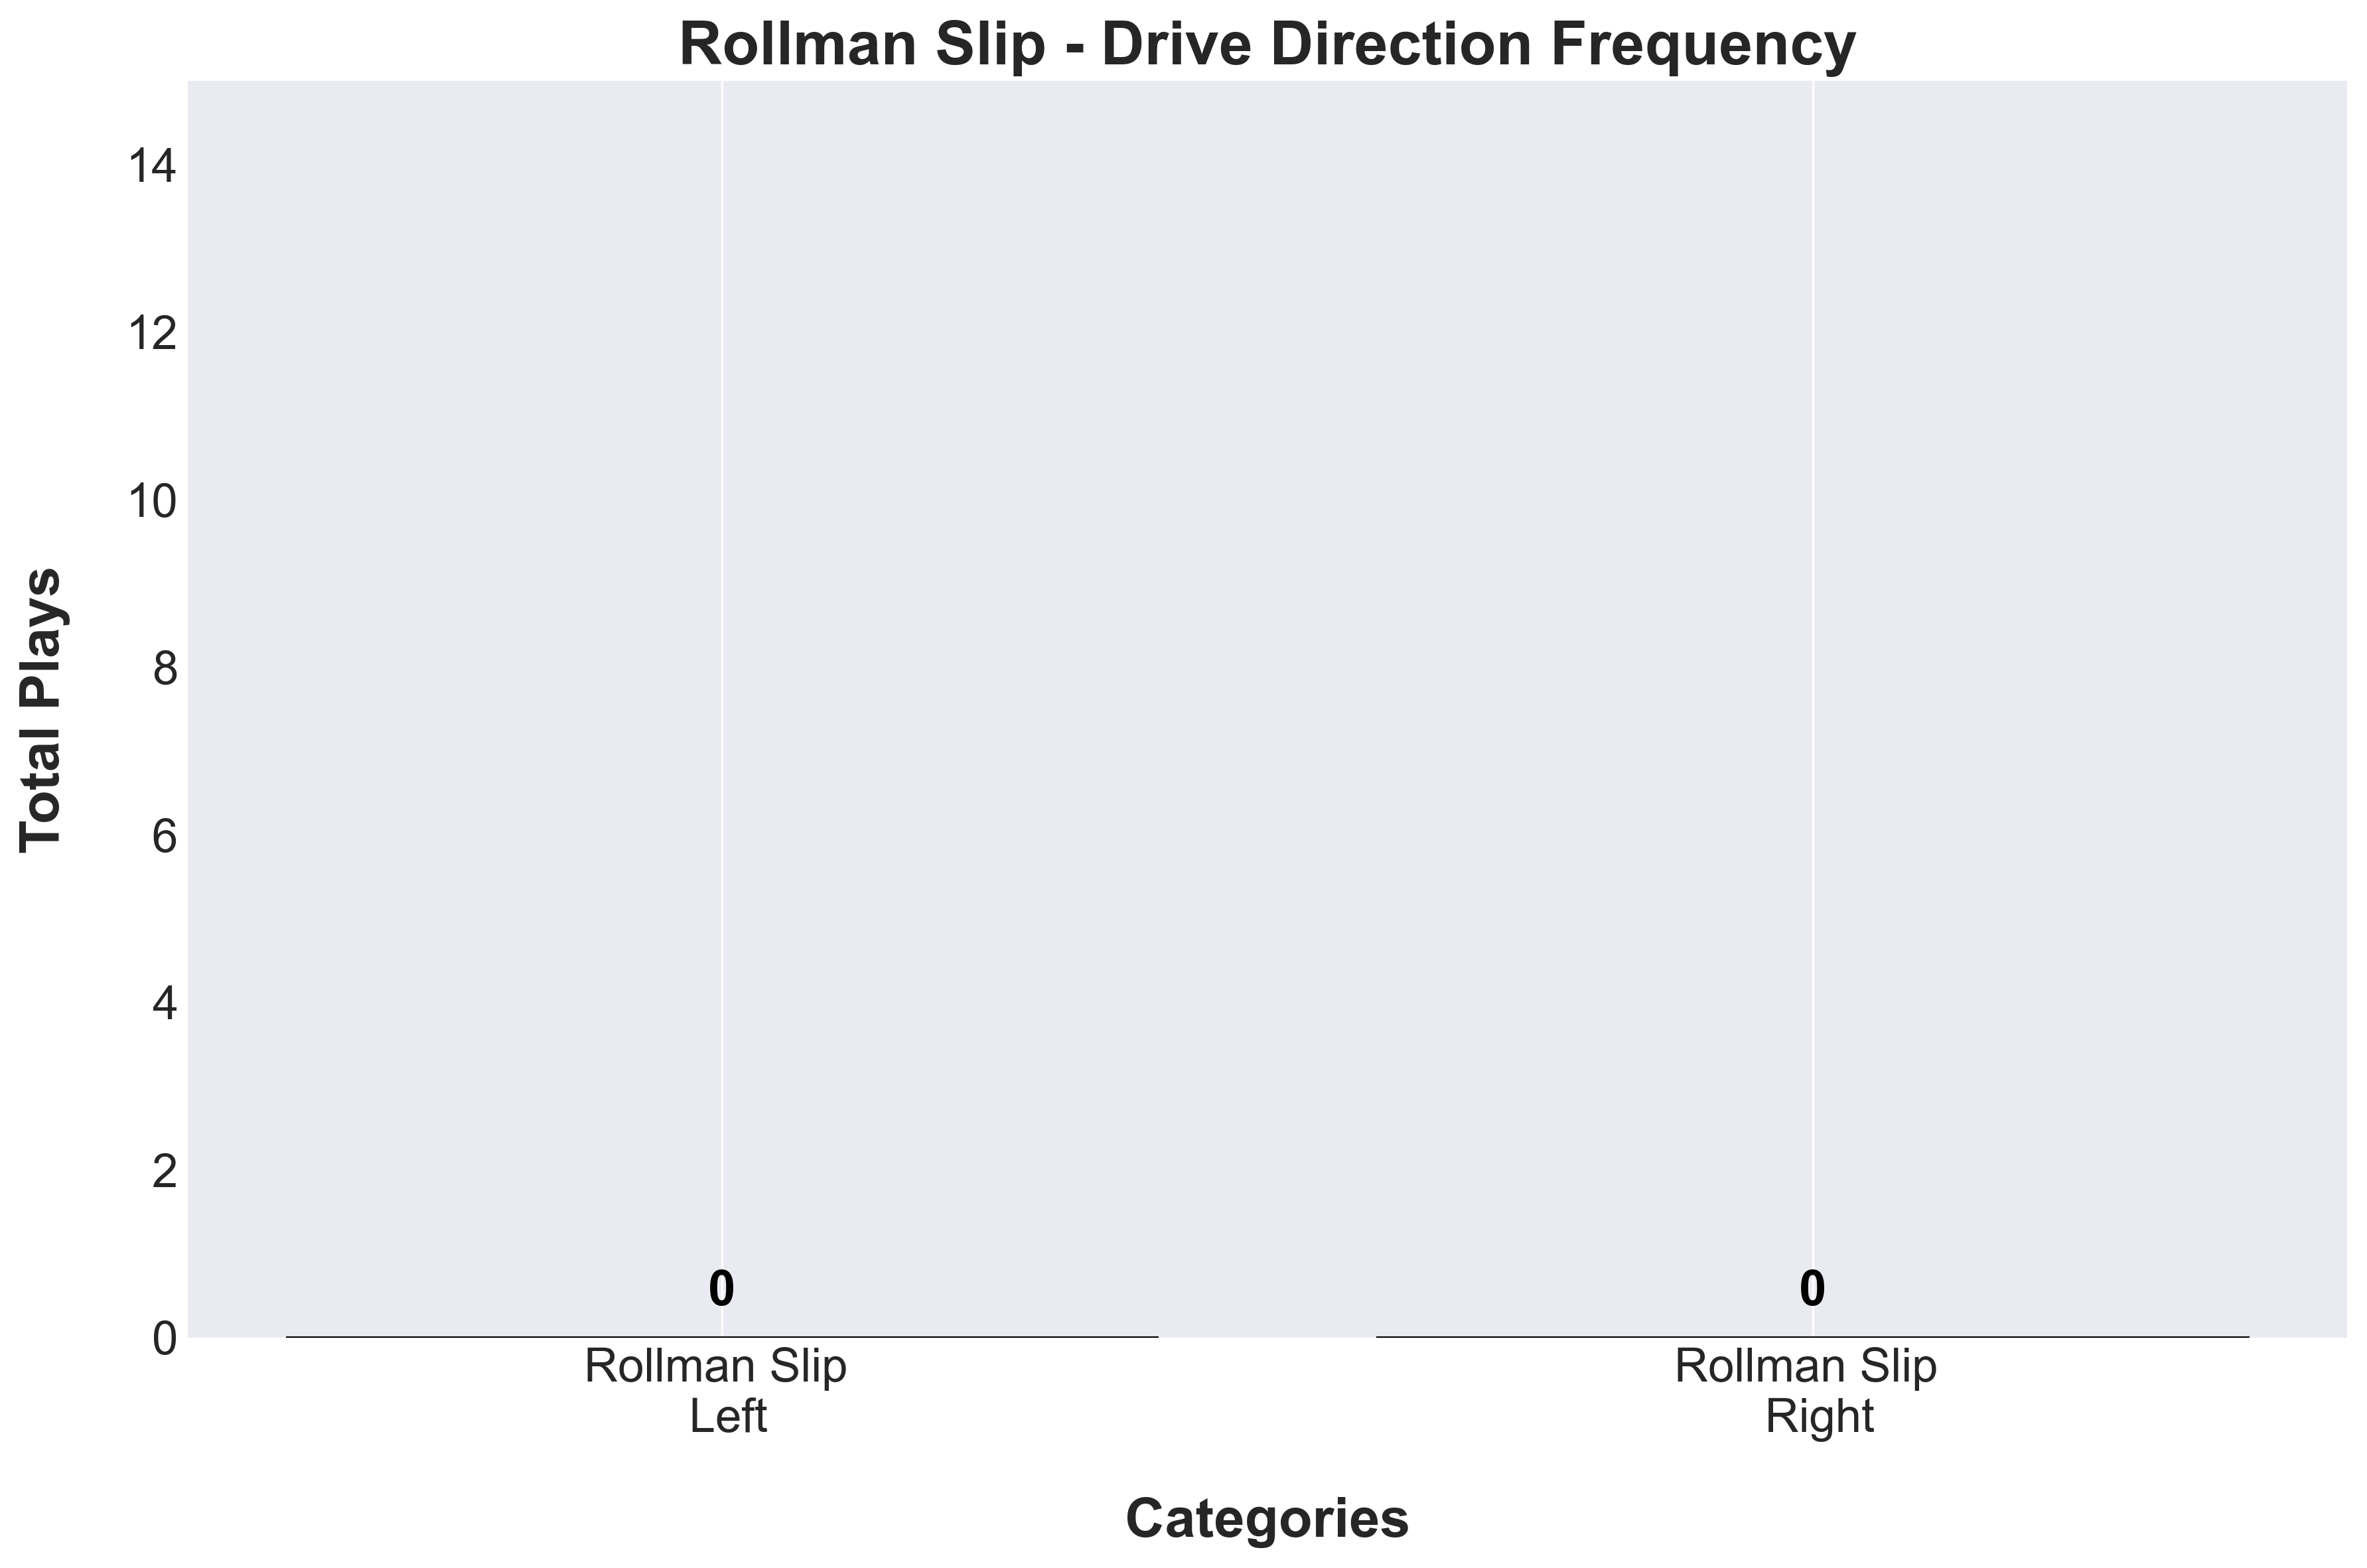
\includegraphics[width=\textwidth, height=.14\textheight]{images/Rollman_SlipDirection_Freq.png} % Adjust the width of the image to fit
    \end{minipage}
    
\end{table}

\vspace{-1em} % Add vertical space before the line (optional)
%\hrule height 1pt width 1\textwidth % Adjust height and width
\vspace{-1em} % Add vertical space after the line (optional)

% Rollman Pop Drive Direction
\begin{table}[H]
    \raisebox{3.5em}{ % Adjust this value to shift the tables vertically
    \begin{minipage}[t]{0.6\textwidth} % Left side (table) takes 85% of the width
        \flushleft
        \centering % Centering the title and the table
        \text{Rollman Pop to Drive Direction Statistics} % Title above the table in bold
        \vskip .25em % Adds vertical space between title and table
        \scalebox{.6}{ % Scale the entire table down by half
            \renewcommand{\arraystretch}{1.4} % Adjust the number to increase or decrease row spacing
            \begin{tabular}{
            >{\centering\arraybackslash}p{1.75cm} 
            >{\centering\arraybackslash}p{.75cm} 
            >{\centering\arraybackslash}p{.75cm} 
            >{\centering\arraybackslash}p{.75cm} 
            >{\centering\arraybackslash}p{.75cm}
            >{\centering\arraybackslash}p{.75cm} 
            >{\centering\arraybackslash}p{.75cm} 
            >{\centering\arraybackslash}p{.75cm} 
            >{\centering\arraybackslash}p{.75cm}
            >{\centering\arraybackslash}p{.75cm} 
            >{\centering\arraybackslash}p{.75cm} 
            >{\centering\arraybackslash}p{.75cm}}% Adjust column widths
            \toprule
            {\scriptsize \textbf{PlayType}} &
            {\scriptsize \textbf{Plays}} &
            {\scriptsize \textbf{3PA}} &
            {\scriptsize \textbf{3PM}} &
            {\scriptsize \textbf{3P\%}} & 
            {\scriptsize \textbf{2PA}} & 
            {\scriptsize \textbf{2PM}} & 
            {\scriptsize \textbf{2P\%}} & 
            {\scriptsize \textbf{MiA}} & 
            {\scriptsize \textbf{MiM}} &
            {\scriptsize \textbf{TO}} &
            {\scriptsize \textbf{Foul}} \\
            \midrule
            
                
            
                
            
                
            
                
            
                
            
                
            
                
            
                
            
                
            
                
            
                
            
                
            
                
            
                
            
                
            
                
            


            \bottomrule
        \end{tabular}
        } % End of \scalebox
    \end{minipage}
    } % End of raisebox, closing the adjustment
    \hfill
    \begin{minipage}[c]{0.35\textwidth} % Right side (image) takes 10% of the width
        \flushright
        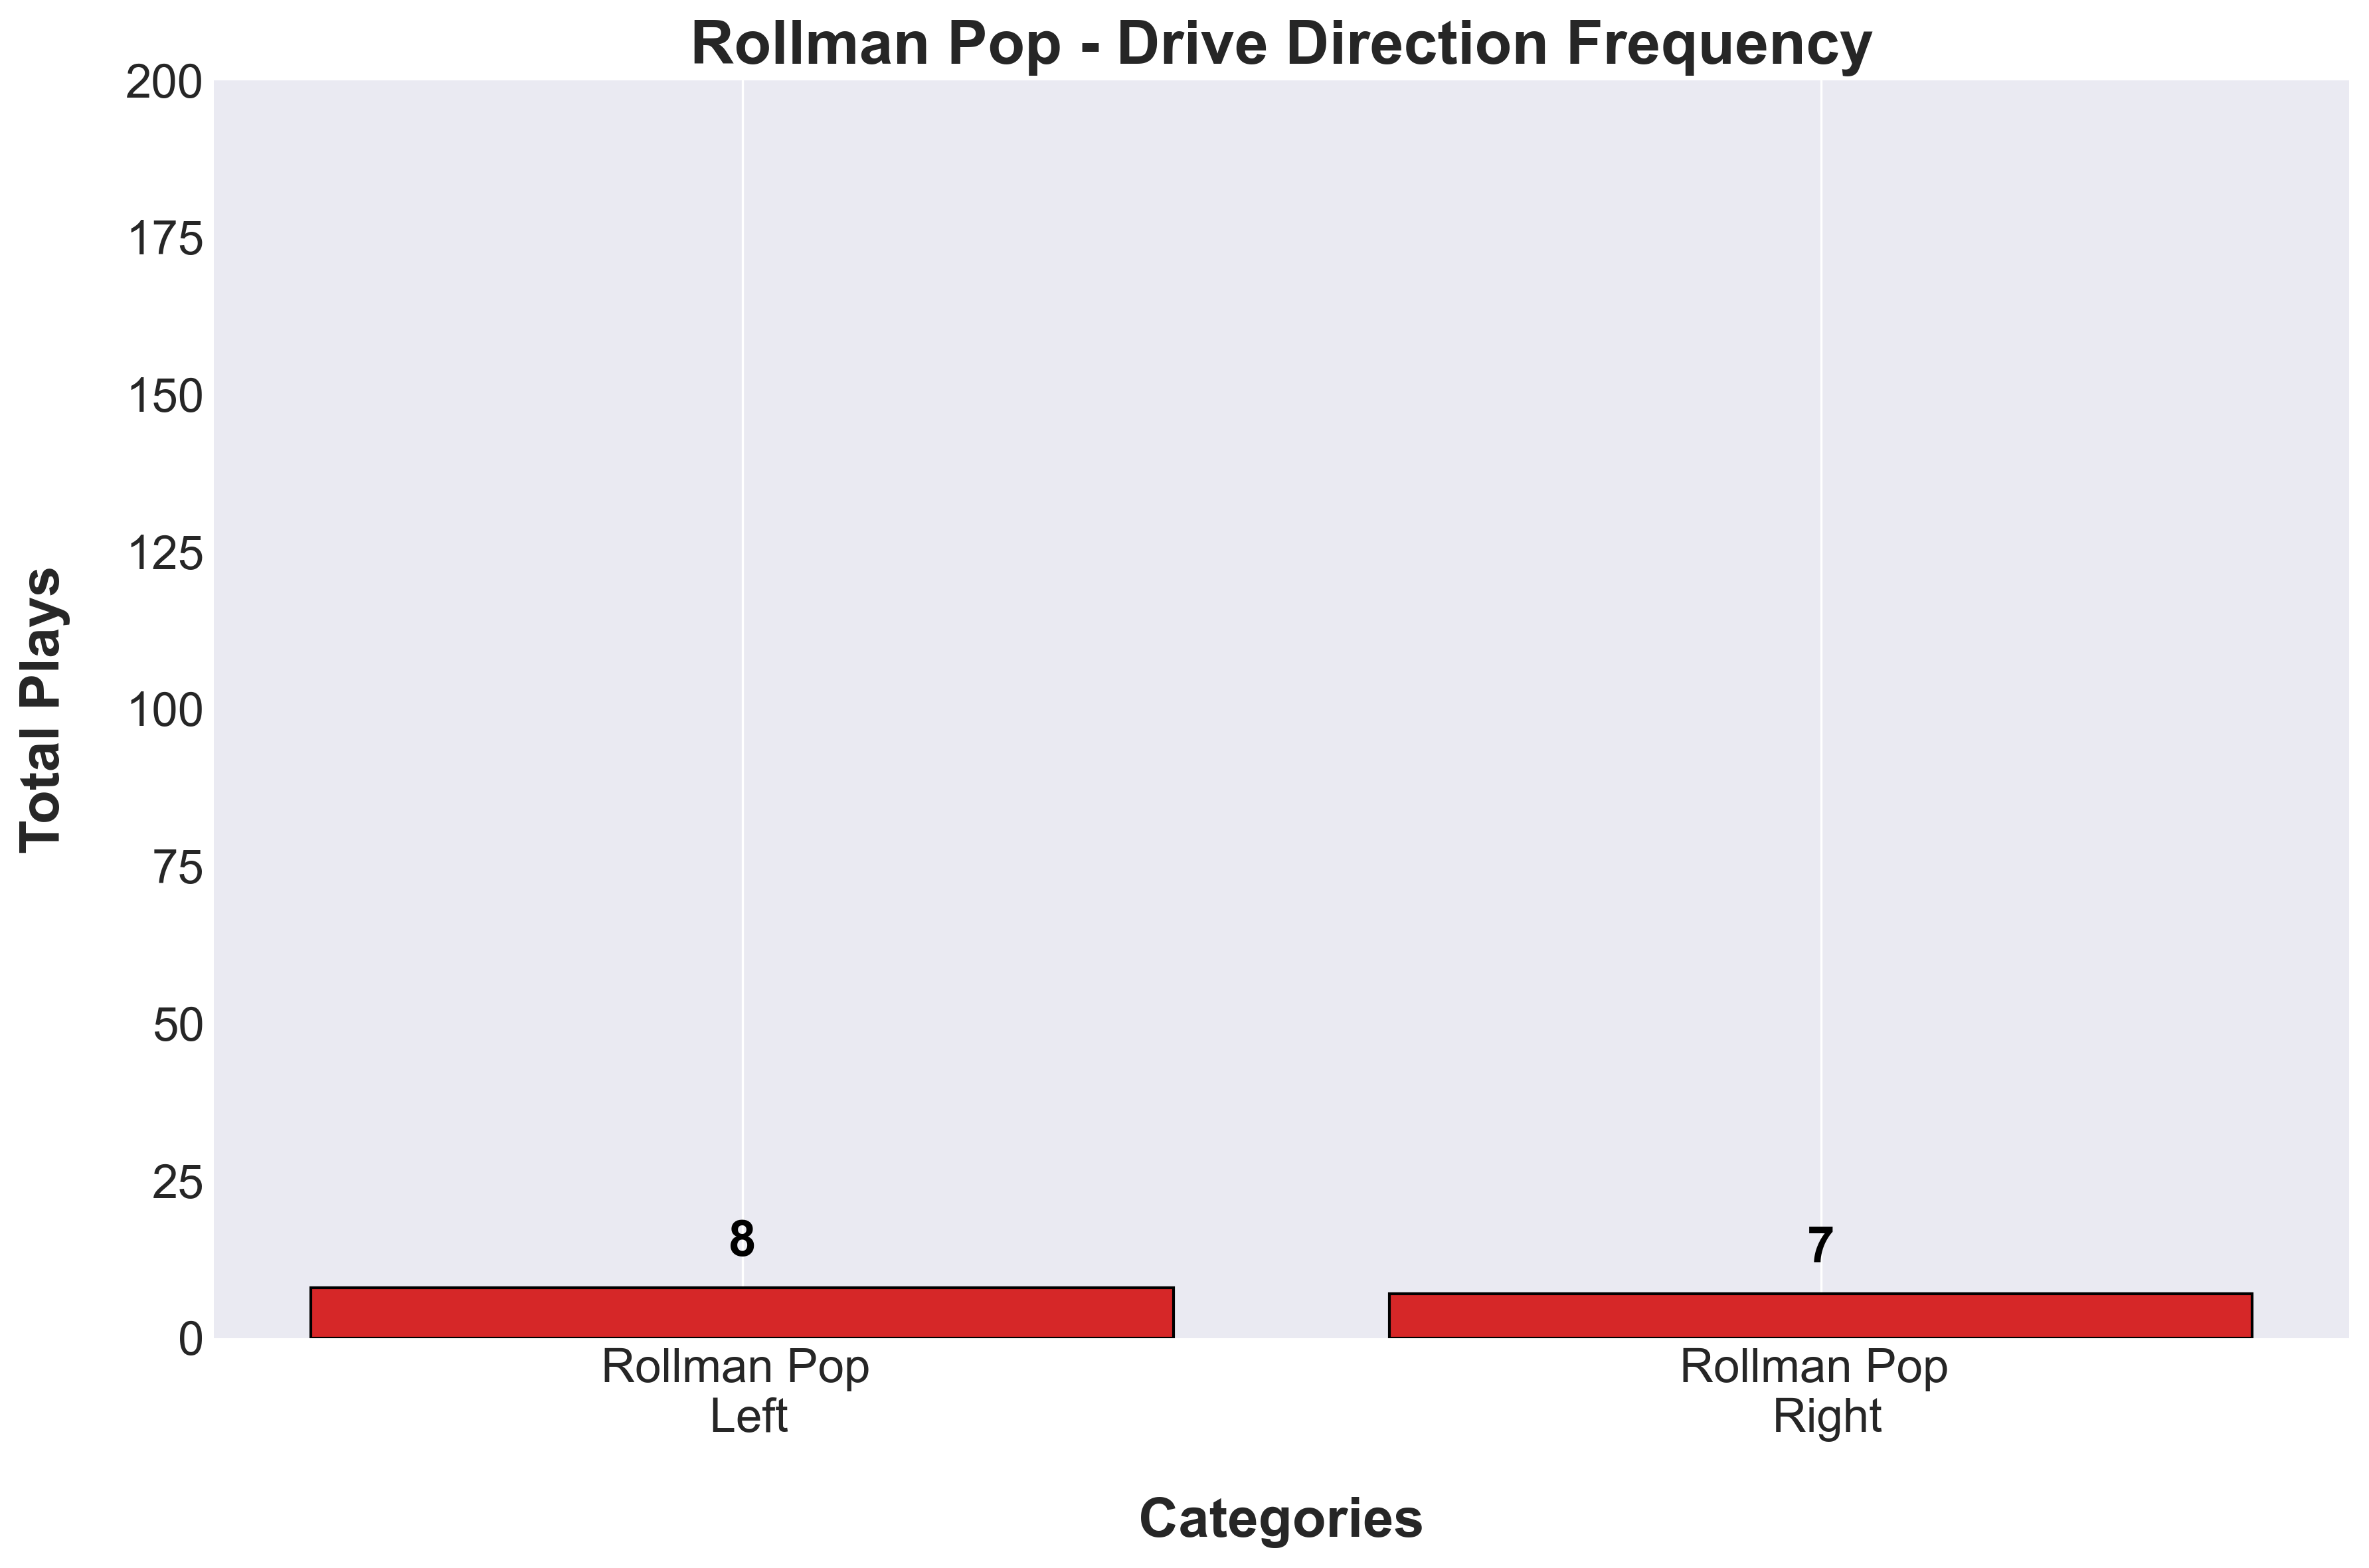
\includegraphics[width=\textwidth, height=.14\textheight]{images/Rollman_PopDirection_Freq.png} % Adjust the width of the image to fit
    \end{minipage}
    
\end{table}

\vspace{-1em} % Add vertical space before the line (optional)
\hrule height 1pt width 1\textwidth % Adjust height and width
\vspace{1em} % Add vertical space after the line (optional)

\subsubsection{Rollman by Passer Statistics}

\vspace{-1em} % Add vertical space before the line (optional)

% Rollman Slips Stats by Passer
\begin{table}[H]
    \raisebox{3em}{ % Adjust this value to shift the tables vertically
    \begin{minipage}[t]{0.6\textwidth} % Left side (table) takes 85% of the width
        \flushleft
        \centering % Centering the title and the table
        \text{Rollman Slip Stats by Passer} % Title above the table in bold
        \vskip .25em % Adds vertical space between title and table
        \scalebox{.55}{ % Scale the entire table down by half
            \renewcommand{\arraystretch}{1.4} % Adjust the number to increase or decrease row spacing
            \begin{tabular}{
            >{\centering\arraybackslash}p{3cm} 
            >{\centering\arraybackslash}p{.75cm} 
            >{\centering\arraybackslash}p{.75cm} 
            >{\centering\arraybackslash}p{.75cm} 
            >{\centering\arraybackslash}p{.75cm}
            >{\centering\arraybackslash}p{.75cm} 
            >{\centering\arraybackslash}p{.75cm} 
            >{\centering\arraybackslash}p{.75cm} 
            >{\centering\arraybackslash}p{.75cm}
            >{\centering\arraybackslash}p{.75cm} 
            >{\centering\arraybackslash}p{.75cm}
            >{\centering\arraybackslash}p{.75cm} 
            >{\centering\arraybackslash}p{.75cm}}% Adjust column widths
            \toprule
            {\scriptsize \textbf{Player}} &
            {\scriptsize \textbf{Plays}} &
            {\scriptsize \textbf{3PA}} &
            {\scriptsize \textbf{3PM}} &
            {\scriptsize \textbf{3P\%}} & 
            {\scriptsize \textbf{2PA}} & 
            {\scriptsize \textbf{2PM}} & 
            {\scriptsize \textbf{2P\%}} & 
            {\scriptsize \textbf{MiA}} & 
            {\scriptsize \textbf{MiM}} &
            {\scriptsize \textbf{Mi\%}} &
            {\scriptsize \textbf{TO}} &
            {\scriptsize \textbf{Foul}} \\
            \midrule
            
                
            
                
            
                
            
                
            
                
            
                
            
                
            
                
            
                
            
                
            
                
            
                
            
                
            
                
                    
                
            
                
            
                
            

            \bottomrule
        \end{tabular}
        } % End of \scalebox
    \end{minipage}
    } % End of raisebox, closing the adjustment
    \hfill % This adds some flexible space between the table and the image
    \begin{minipage}[c]{0.35\textwidth} % Right side (image) takes 10% of the width
        \flushright
        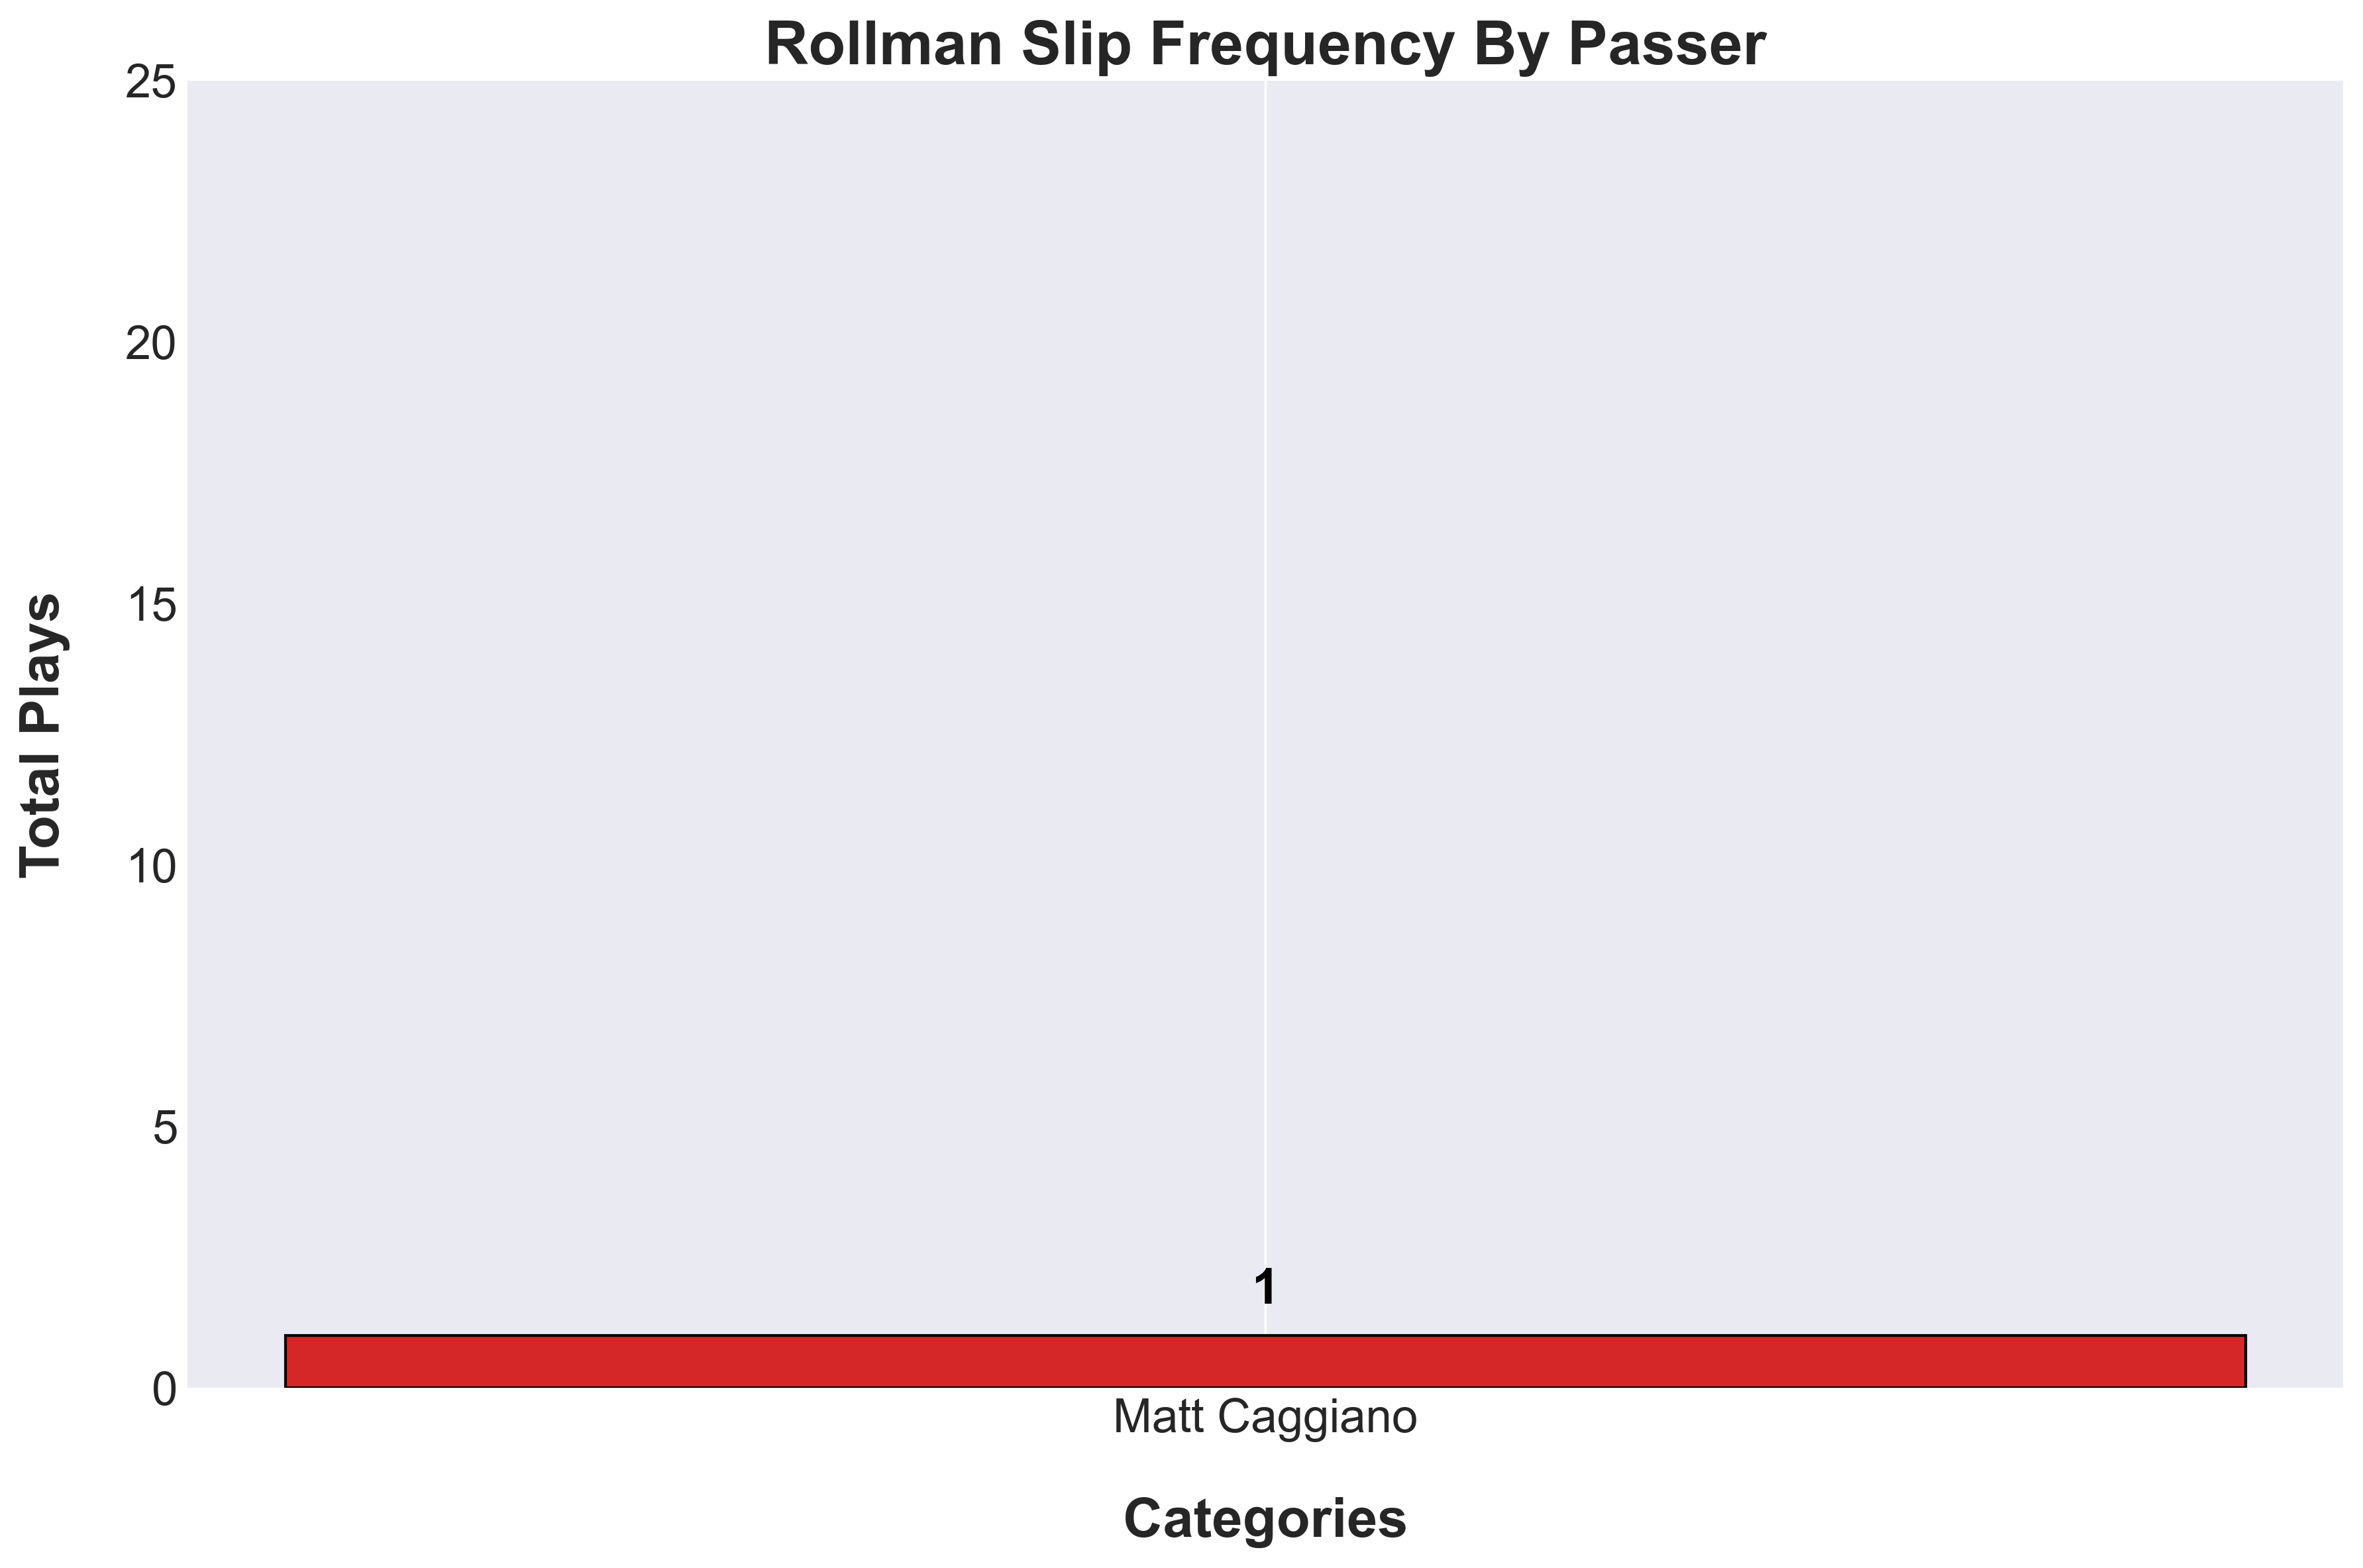
\includegraphics[width=\textwidth, height=.14\textheight]{images/Rollman_SlipPlayer_Freq.png} % Adjust the width of the image to fit
    \end{minipage}
\end{table}

\vspace{-1em} % Add vertical space before the line (optional)
\vspace{-1em} % Add vertical space after the line (optional)

% Rollman Pop Stats by Passer
\begin{table}[H]
    \raisebox{3em}{ % Adjust this value to shift the tables vertically
    \begin{minipage}[t]{0.6\textwidth} % Left side (table) takes 85% of the width
        \flushleft
        \centering % Centering the title and the table
        \text{Rollman Pop Stats by Passer} % Title above the table in bold
        \vskip .25em % Adds vertical space between title and table
        \scalebox{.55}{ % Scale the entire table down by half
            \renewcommand{\arraystretch}{1.4} % Adjust the number to increase or decrease row spacing
            \begin{tabular}{
            >{\centering\arraybackslash}p{3cm} 
            >{\centering\arraybackslash}p{.75cm} 
            >{\centering\arraybackslash}p{.75cm} 
            >{\centering\arraybackslash}p{.75cm} 
            >{\centering\arraybackslash}p{.75cm}
            >{\centering\arraybackslash}p{.75cm} 
            >{\centering\arraybackslash}p{.75cm} 
            >{\centering\arraybackslash}p{.75cm} 
            >{\centering\arraybackslash}p{.75cm}
            >{\centering\arraybackslash}p{.75cm} 
            >{\centering\arraybackslash}p{.75cm}
            >{\centering\arraybackslash}p{.75cm} 
            >{\centering\arraybackslash}p{.75cm}}% Adjust column widths
            \toprule
            {\scriptsize \textbf{Player}} &
            {\scriptsize \textbf{Plays}} &
            {\scriptsize \textbf{3PA}} &
            {\scriptsize \textbf{3PM}} &
            {\scriptsize \textbf{3P\%}} & 
            {\scriptsize \textbf{2PA}} & 
            {\scriptsize \textbf{2PM}} & 
            {\scriptsize \textbf{2P\%}} & 
            {\scriptsize \textbf{MiA}} & 
            {\scriptsize \textbf{MiM}} &
            {\scriptsize \textbf{Mi\%}} &
            {\scriptsize \textbf{TO}} &
            {\scriptsize \textbf{Foul}} \\
            \midrule
            
                
            
                
            
                
            
                
            
                
            
                
            
                
            
                
            
                
            
                
            
                
            
                
            
                
            
                
            
                
                    
                
            
                
            

            \bottomrule
        \end{tabular}
        } % End of \scalebox
    \end{minipage}
    } % End of raisebox, closing the adjustment
    \hfill % This adds some flexible space between the table and the image
    \begin{minipage}[c]{0.35\textwidth} % Right side (image) takes 10% of the width
        \flushright
        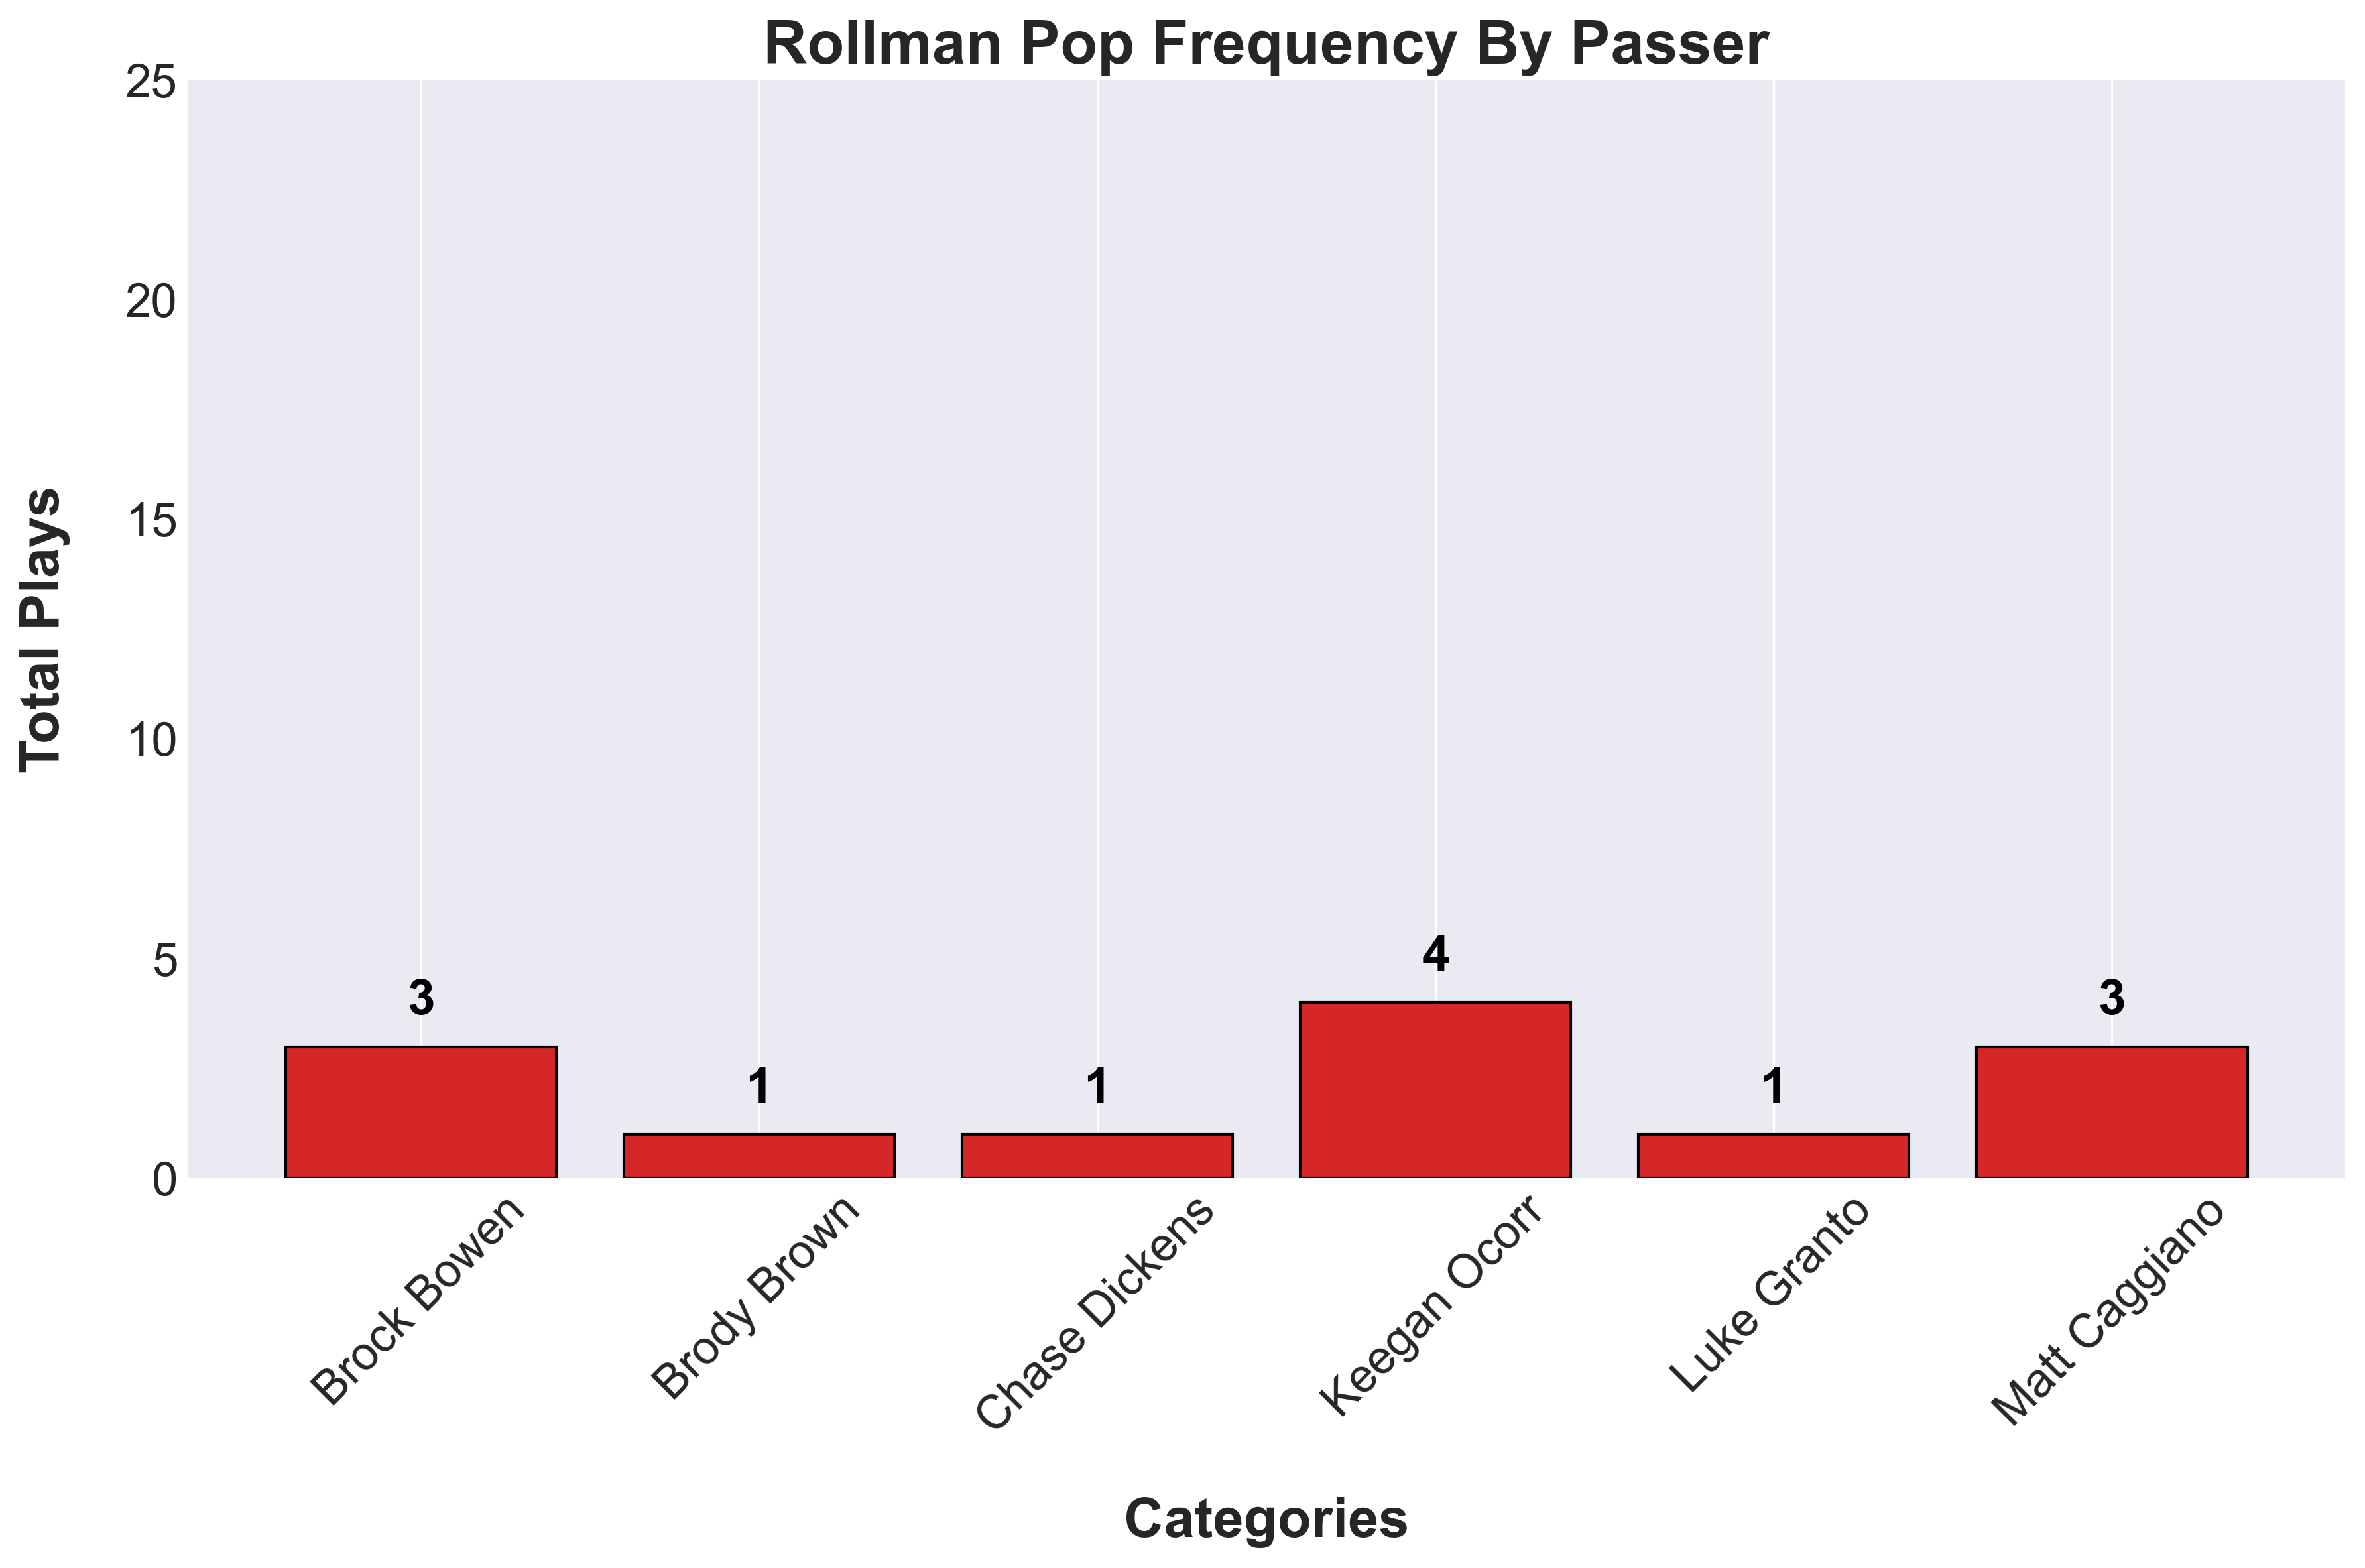
\includegraphics[width=\textwidth, height=.14\textheight]{images/Rollman_PopPlayer_Freq.png} % Adjust the width of the image to fit
    \end{minipage}
\end{table}

\vspace{-1em} % Add vertical space before the line (optional)
\vspace{-1em} % Add vertical space after the line (optional)

% Rollman Rolls Stats by Passer
\begin{table}[H]
    \raisebox{3em}{ % Adjust this value to shift the tables vertically
    \begin{minipage}[t]{0.6\textwidth} % Left side (table) takes 85% of the width
        \flushleft
        \centering % Centering the title and the table
        \text{Rollman Roll Stats by Passer} % Title above the table in bold
        \vskip .25em % Adds vertical space between title and table
        \scalebox{.55}{ % Scale the entire table down by half
            \renewcommand{\arraystretch}{1.4} % Adjust the number to increase or decrease row spacing
            \begin{tabular}{
            >{\centering\arraybackslash}p{3cm} 
            >{\centering\arraybackslash}p{.75cm} 
            >{\centering\arraybackslash}p{.75cm} 
            >{\centering\arraybackslash}p{.75cm} 
            >{\centering\arraybackslash}p{.75cm}
            >{\centering\arraybackslash}p{.75cm} 
            >{\centering\arraybackslash}p{.75cm} 
            >{\centering\arraybackslash}p{.75cm} 
            >{\centering\arraybackslash}p{.75cm}
            >{\centering\arraybackslash}p{.75cm} 
            >{\centering\arraybackslash}p{.75cm}
            >{\centering\arraybackslash}p{.75cm} 
            >{\centering\arraybackslash}p{.75cm}}% Adjust column widths
            \toprule
            {\scriptsize \textbf{Player}} &
            {\scriptsize \textbf{Plays}} &
            {\scriptsize \textbf{3PA}} &
            {\scriptsize \textbf{3PM}} &
            {\scriptsize \textbf{3P\%}} & 
            {\scriptsize \textbf{2PA}} & 
            {\scriptsize \textbf{2PM}} & 
            {\scriptsize \textbf{2P\%}} & 
            {\scriptsize \textbf{MiA}} & 
            {\scriptsize \textbf{MiM}} &
            {\scriptsize \textbf{Mi\%}} &
            {\scriptsize \textbf{TO}} &
            {\scriptsize \textbf{Foul}} \\
            \midrule
            
                
            
                
            
                
            
                
            
                
            
                
            
                
            
                
            
                
            
                
            
                
            
                
            
                
            
                
            
                
            
                
                    
                
            

            \bottomrule
        \end{tabular}
        } % End of \scalebox
    \end{minipage}
    } % End of raisebox, closing the adjustment
    \hfill % This adds some flexible space between the table and the image
    \begin{minipage}[c]{0.35\textwidth} % Right side (image) takes 10% of the width
        \flushright
        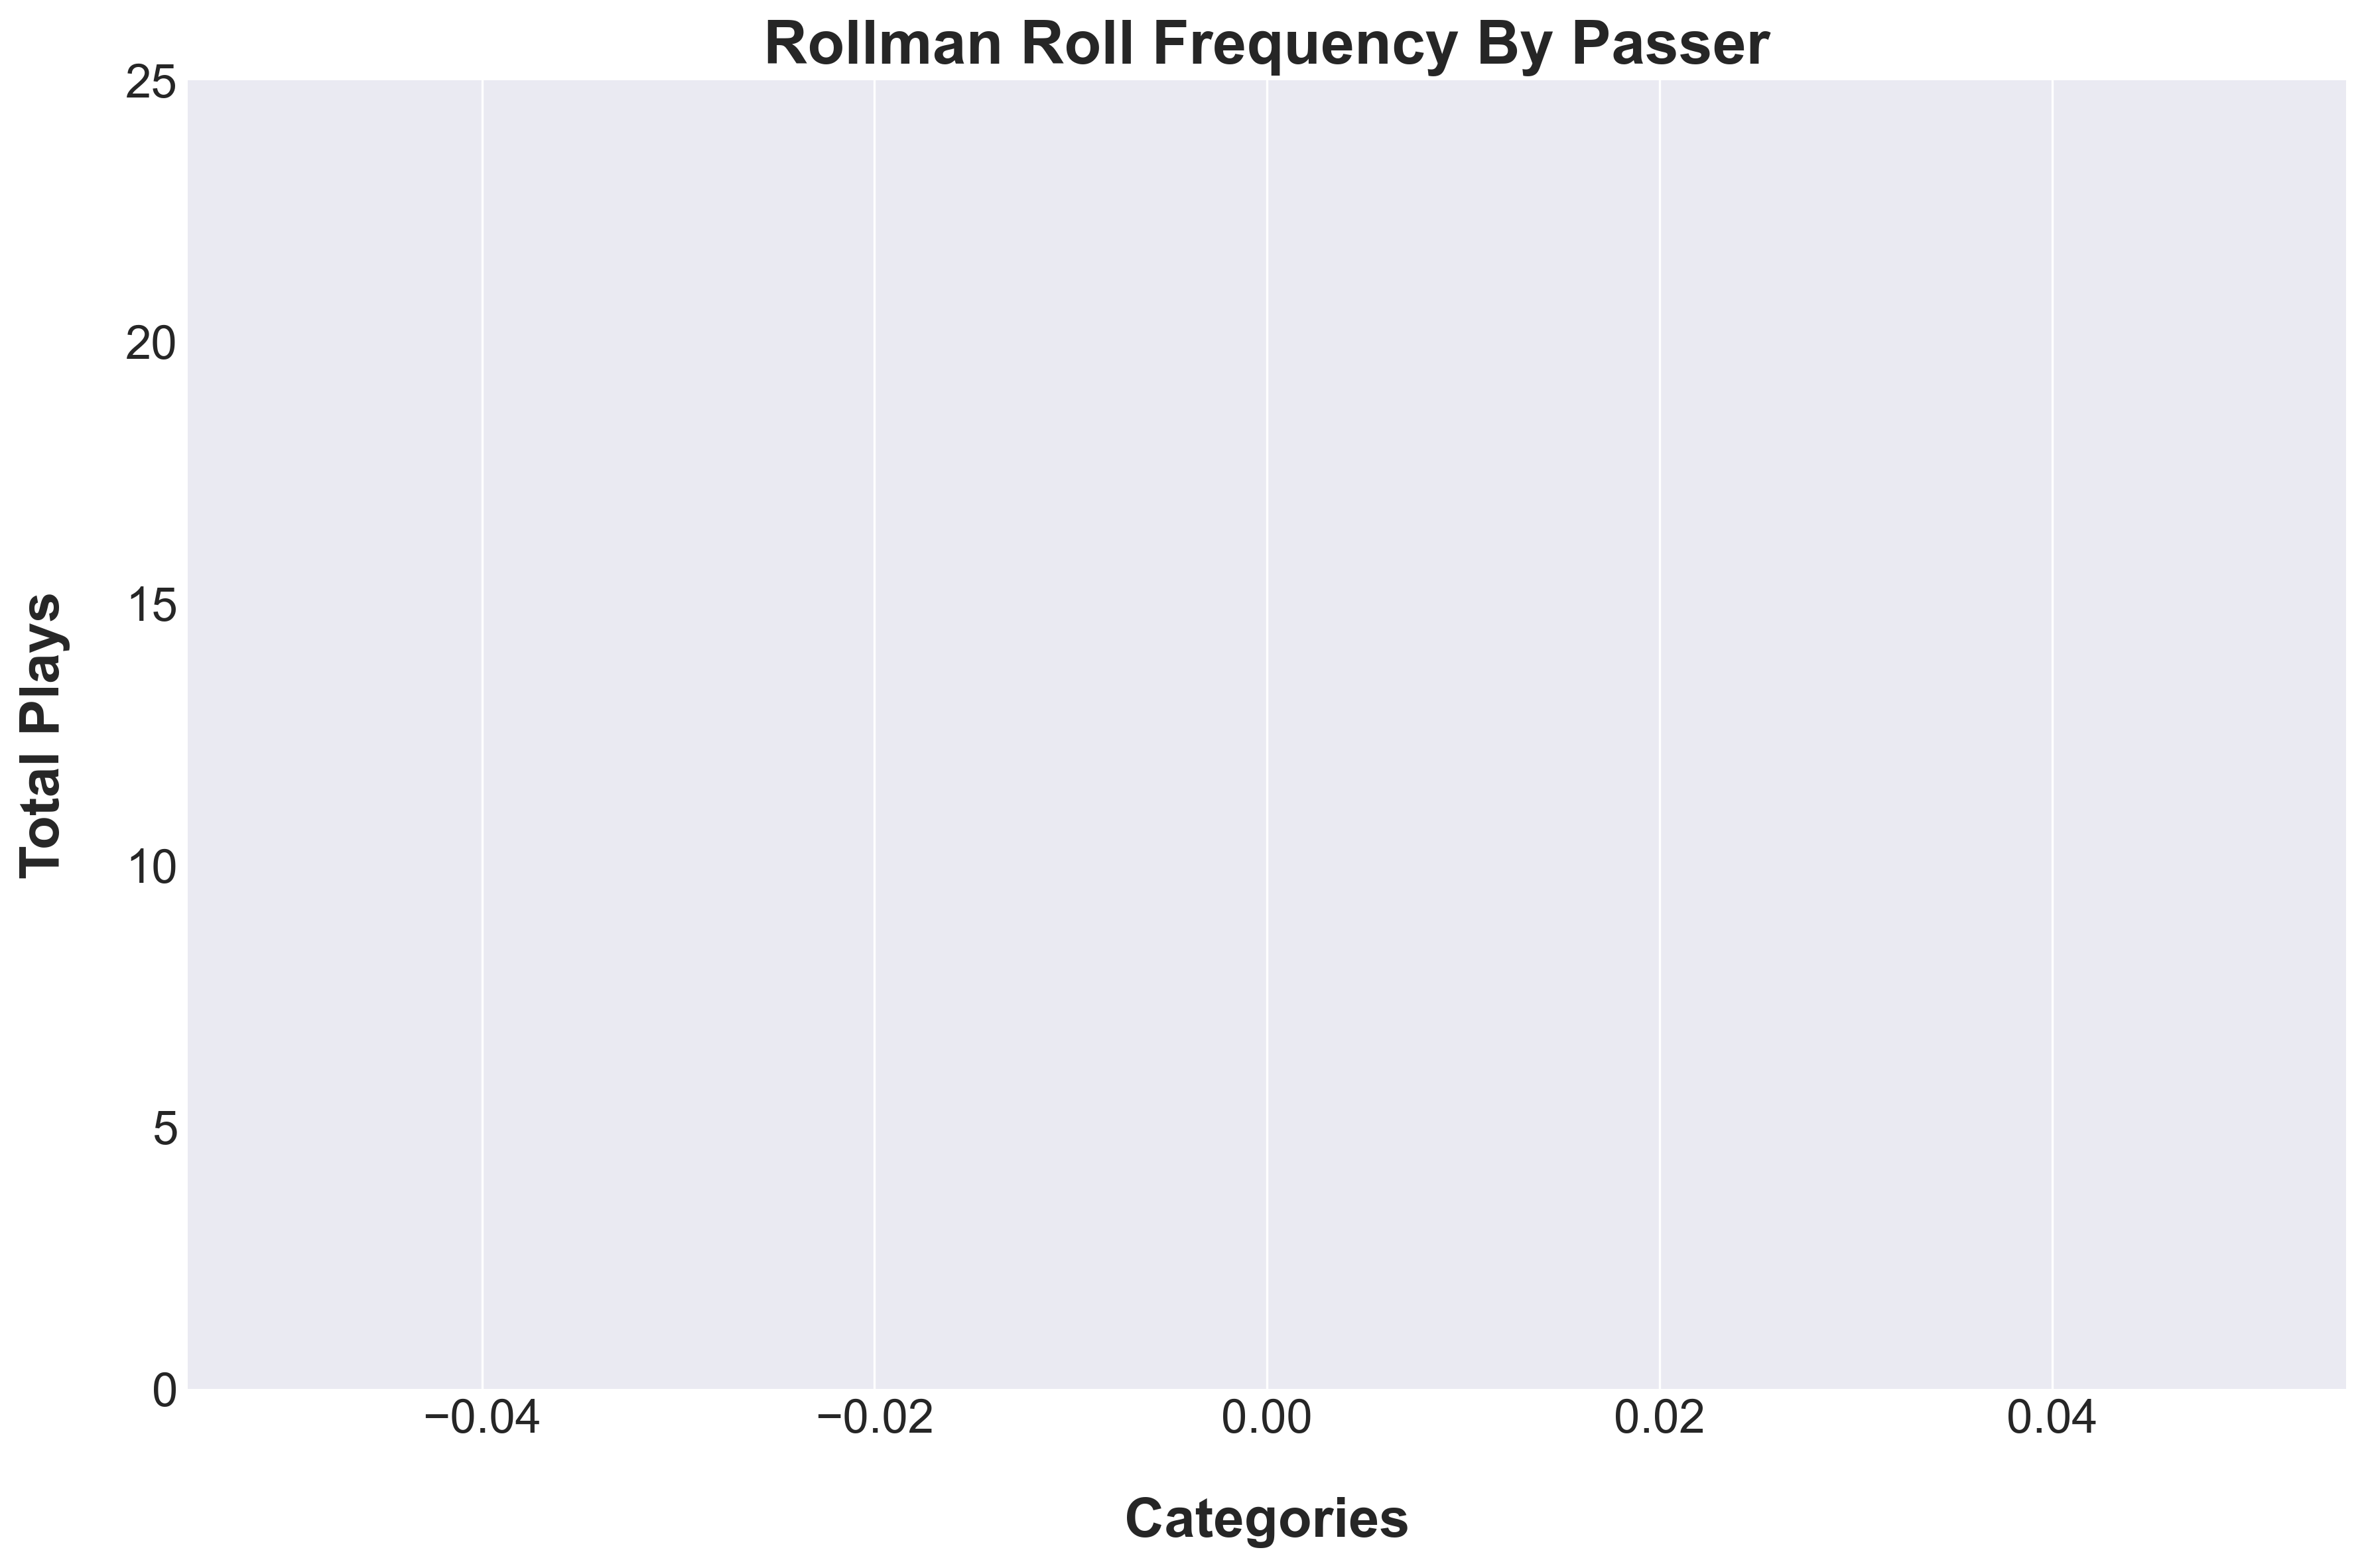
\includegraphics[width=\textwidth, height=.14\textheight]{images/Rollman_RollPlayer_Freq.png} % Adjust the width of the image to fit
    \end{minipage}
\end{table}

\vspace{-1em} % Add vertical space before the line (optional)
\hrule height 1pt width 1\textwidth % Adjust height and width
\vspace{1em} % Add vertical space after the line (optional)

\clearpage

% ----------------------
% Spot Up Visuals and Insights Section
% ----------------------
\subsection{Spot Ups}

\vspace{1.25em} % Add vertical space before the line (optional)
\textbf{Key Notes on Spot up Tendencies}
\vspace{0.5em} % Add space between the title and the itemized list

\begin{itemize}
    \item Spot up Jumpers/Drives make up x\% of players offensive load
    \vspace{0.3em} % Add space between the title and the itemized list
    \item Player is more likely to drive on Spot up plays with x\% of spotup shots coming off drives
\end{itemize}

\vspace{1em} % Add vertical space before the line (optional)
\hrule height 1pt width 1\textwidth % Adjust height and width
\vspace{0em} % Add vertical space after the line (optional)

\subsubsection{Spot Up Shot / Drive Statistics}

% All Spot up Statistics Table w/ room for insights
\begin{table}[H]
    \centering
    \begin{minipage}[t]{0.6\textwidth} % Left side (table) takes 85% of the width
        %\flushright
        \centering % Centering the title and the table
        \text{Total Spot Up Statistics} % Title above the table in bold
        \vskip .25em % Adds vertical space between title and table
        \scalebox{.85}{ % Scale the entire table down by half
            \scriptsize % Reduce the font size
            \begin{tabular}{
            >{\centering\arraybackslash}p{.75cm} 
            >{\centering\arraybackslash}p{.5cm} 
            >{\centering\arraybackslash}p{.5cm} 
            >{\centering\arraybackslash}p{.5cm}
            >{\centering\arraybackslash}p{.5cm} 
            >{\centering\arraybackslash}p{.5cm} 
            >{\centering\arraybackslash}p{.5cm} 
            >{\centering\arraybackslash}p{.5cm}
            >{\centering\arraybackslash}p{.5cm} 
            >{\centering\arraybackslash}p{.5cm}
            >{\centering\arraybackslash}p{.5cm} 
            >{\centering\arraybackslash}p{.5cm}}% Adjust column widths
            \toprule
            \textbf{Plays} &
            \textbf{3PA} &
            \textbf{3PM} &
            \textbf{3P\%} & 
            \textbf{2PA} & 
            \textbf{2PM} & 
            \textbf{2P\%} & 
            \textbf{MiA} & 
            \textbf{MiM} &
            \textbf{Mi\%} &
            \textbf{TO} &
            \textbf{Foul} \\
            \midrule
            
                
            
                
            
                
            
                
            
                
            
                
            
                
            
                
            
                
            
                
            
                
            
                
            
                
            
                
            
                
            
                
                    79 & 33 & 12 &
                    36.36 & 
                    35 & 20 &
                    57.14 &
                    14 & 7 &
                    50.0 &
                    6 & 5 \\
                
            
                
            
                
            
                
            
                
            
                
            
                
            

            \bottomrule
            \end{tabular}
        }
    \end{minipage}
\end{table}

\vspace{0em} % Add vertical space before the line (optional)
%\hrule height 1pt width 1\textwidth % Adjust height and width
\vspace{-1em} % Add vertical space after the line (optional)

% Spot up Stats for Jumpers vs Drives
\begin{table}[H]
    \raisebox{3em}{ % Adjust this value to shift the tables vertically
    \begin{minipage}[t]{0.6\textwidth} % Left side (table) takes 85% of the width
        \flushleft
        \centering % Centering the title and the table
        \text{Spot Up Statistics} % Title above the table in bold
        \vskip .25em % Adds vertical space between title and table
        \scalebox{.6}{ % Scale the entire table down by half
            \renewcommand{\arraystretch}{1.4} % Adjust the number to increase or decrease row spacing
            \begin{tabular}{
            >{\centering\arraybackslash}p{1.75cm} 
            >{\centering\arraybackslash}p{.75cm} 
            >{\centering\arraybackslash}p{.75cm} 
            >{\centering\arraybackslash}p{.75cm} 
            >{\centering\arraybackslash}p{.75cm}
            >{\centering\arraybackslash}p{.75cm} 
            >{\centering\arraybackslash}p{.75cm} 
            >{\centering\arraybackslash}p{.75cm} 
            >{\centering\arraybackslash}p{.75cm}
            >{\centering\arraybackslash}p{.75cm} 
            >{\centering\arraybackslash}p{.75cm}
            >{\centering\arraybackslash}p{.75cm} 
            >{\centering\arraybackslash}p{.75cm}}% Adjust column widths
            \toprule
            {\scriptsize \textbf{PlayType}} &
            {\scriptsize \textbf{Plays}} &
            {\scriptsize \textbf{3PA}} &
            {\scriptsize \textbf{3PM}} &
            {\scriptsize \textbf{3P\%}} & 
            {\scriptsize \textbf{2PA}} & 
            {\scriptsize \textbf{2PM}} & 
            {\scriptsize \textbf{2P\%}} & 
            {\scriptsize \textbf{MiA}} & 
            {\scriptsize \textbf{MiM}} &
            {\scriptsize \textbf{Mi\%}} &
            {\scriptsize \textbf{TO}} &
            {\scriptsize \textbf{Foul}} \\
            \midrule
            
                
            
                
            
                
            
                
            
                
            
                
            
                
            
                
            
                
            
                
            
                
            
                
            
                
            
                
            
                
            
                
            
                
            
                
                    Jumpshot & 34 & 33 & 12 &
                    36.36 & 
                    0 & 0 &
                    - &
                    0 & 0 &
                    - &
                    0 & 1 \\
                
            
                
                    Drive & 45 & 0 & 0 &
                    - & 
                    35 & 20 &
                    48.89 &
                    14 & 7 &
                    50.95 &
                    6 & 4 \\
                
            
                
            
                
            
                
            


            \bottomrule
        \end{tabular}
        } % End of \scalebox
    \end{minipage}
    } % End of raisebox, closing the adjustment
    \hfill % This adds some flexible space between the table and the image
    \begin{minipage}[c]{0.35\textwidth} % Right side (image) takes 10% of the width
        \flushright
        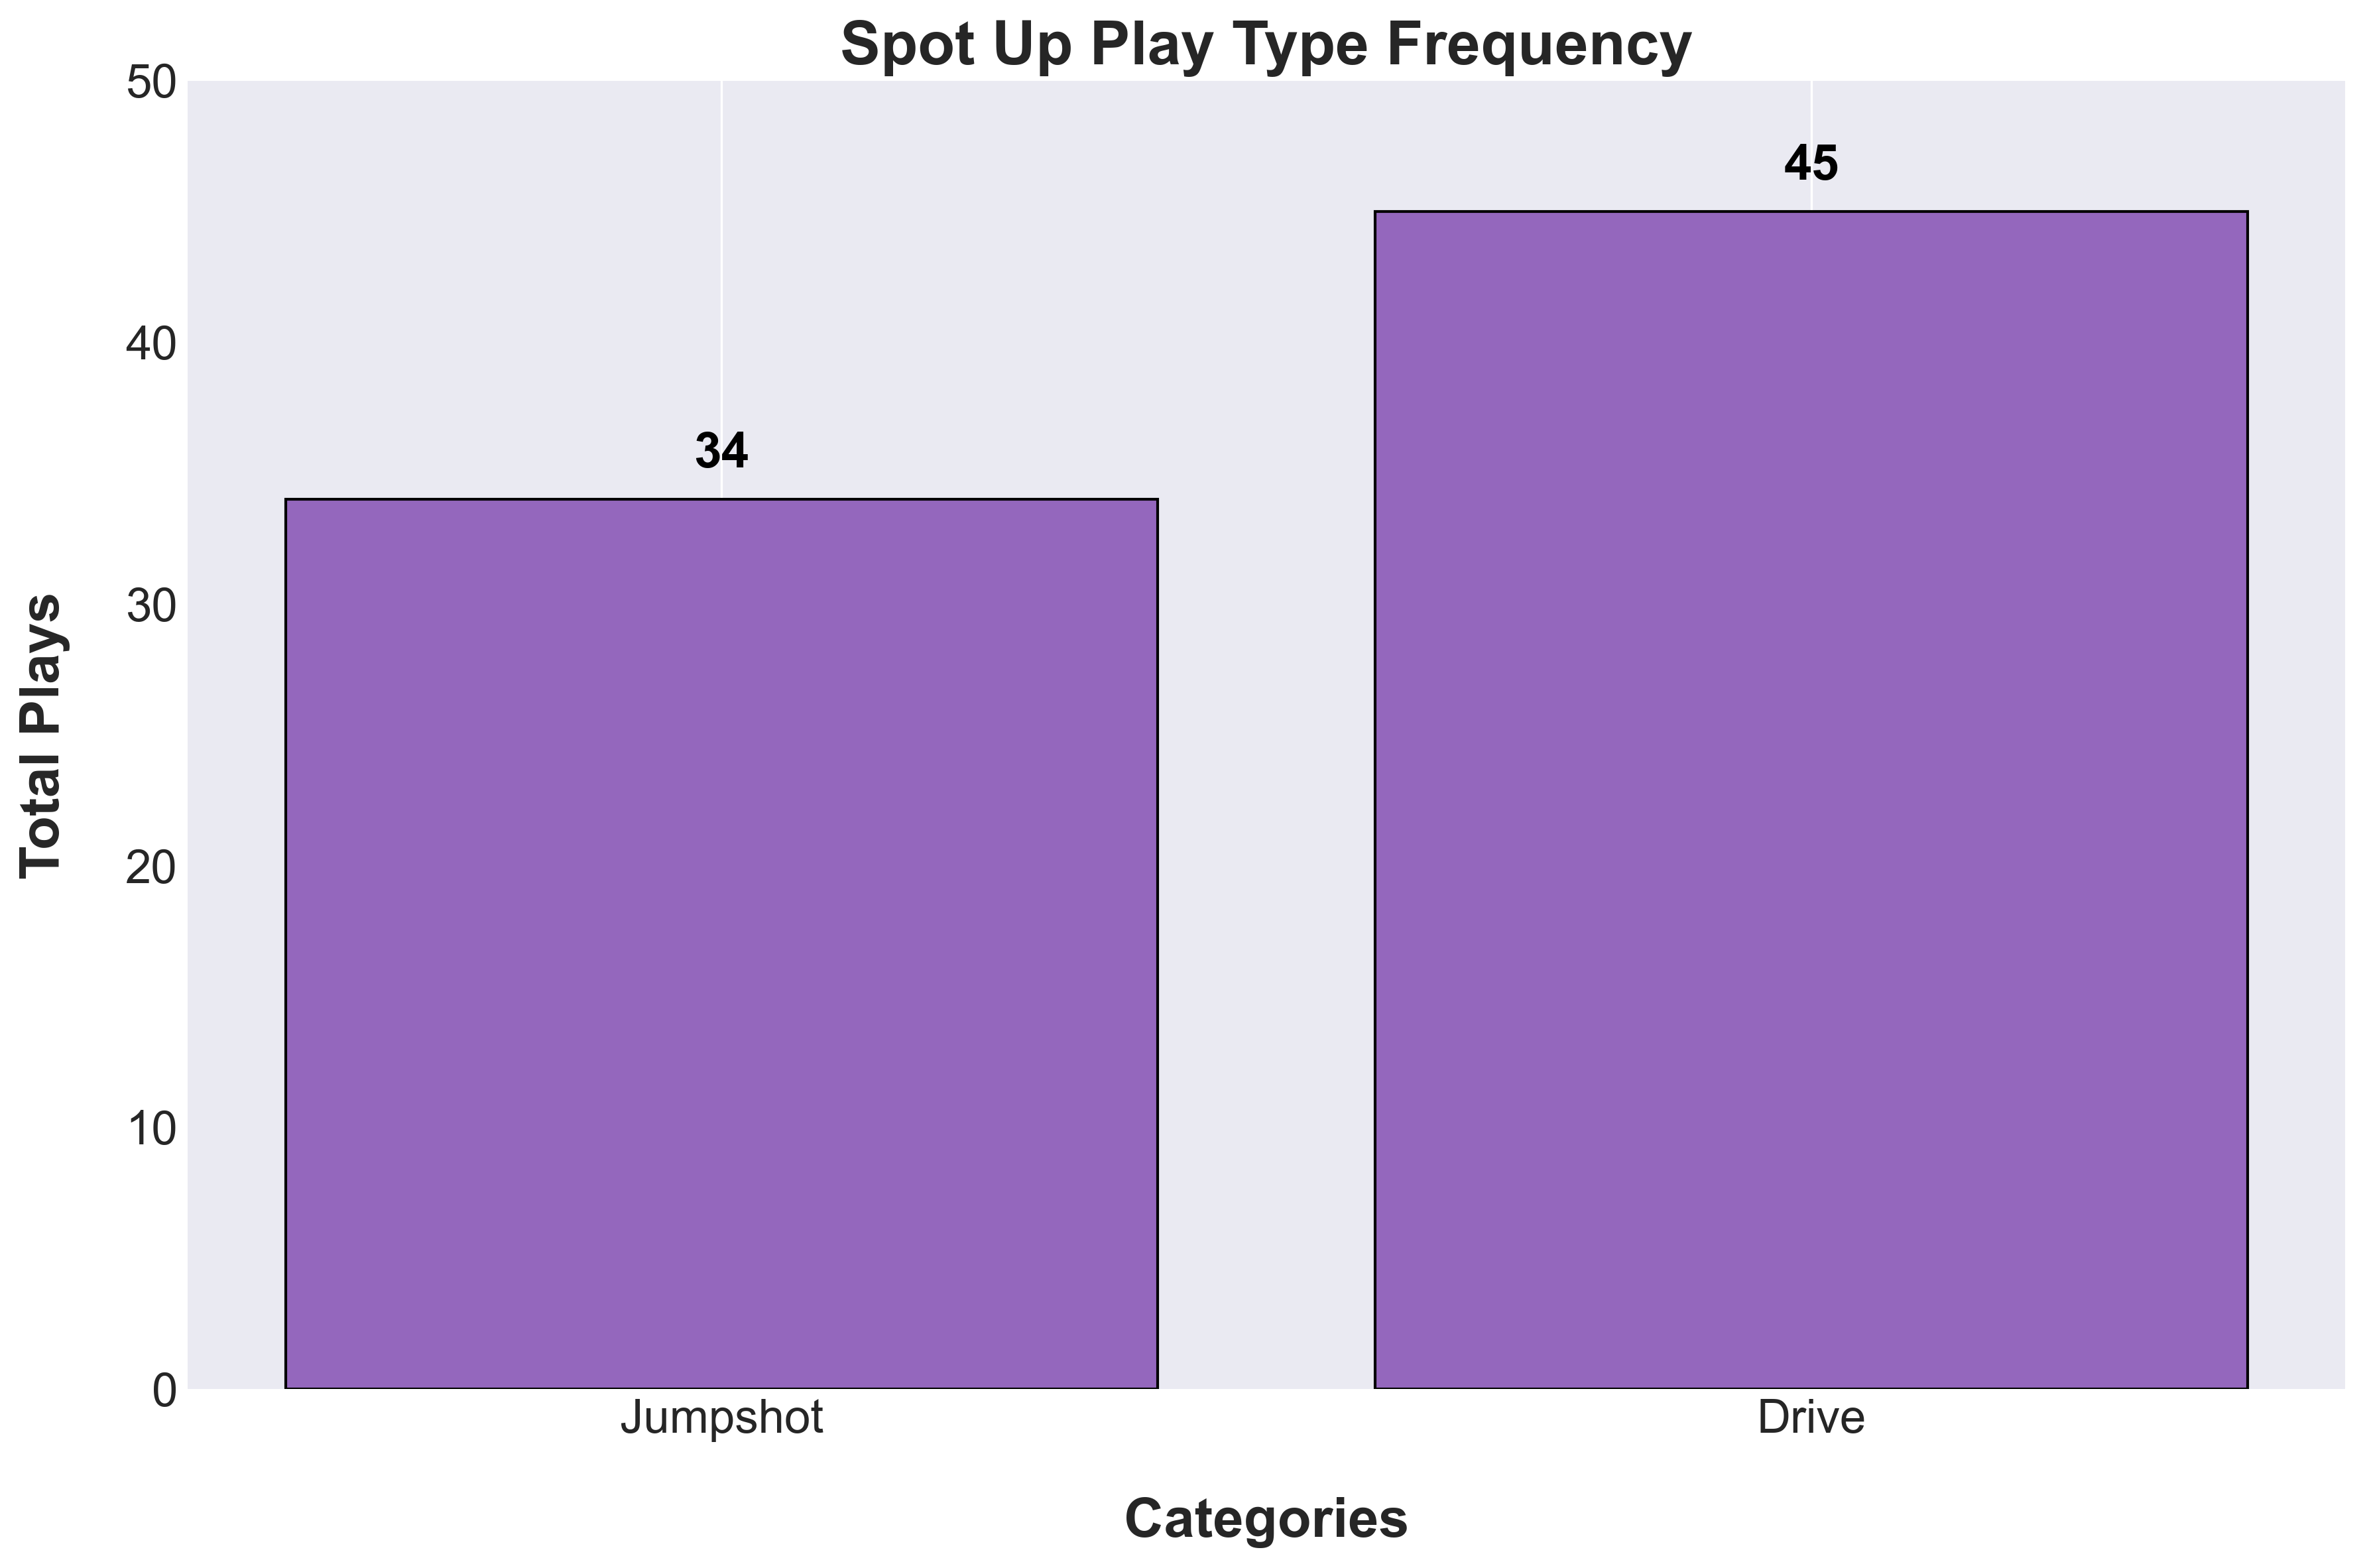
\includegraphics[width=\textwidth, height=.14\textheight]{images/SpotUp_PlayType_Freq.png} % Adjust the width of the image to fit
    \end{minipage}
\end{table}

\vspace{-1em} % Add vertical space before the line (optional)
%\hrule height 1pt width 1\textwidth % Adjust height and width
\vspace{-1em} % Add vertical space after the line (optional)

% Spot up Drives, Left vs Right vs Straight
\begin{table}[H]
    \raisebox{3.5em}{ % Adjust this value to shift the tables vertically
    \centering
    \begin{minipage}[t]{0.6\textwidth} % Left side (table) takes 85% of the width
        \centering % Centering the title and the table
        \text{Drive Direction Statistics} % Title above the table in bold
        \vskip .25em % Adds vertical space between title and table
        \scalebox{.9}{ % Scale the entire table down by half
            \scriptsize % Reduce the font size
            \renewcommand{\arraystretch}{1.4} % Adjust the number to increase or decrease row spacing
            \begin{tabular}{
            >{\centering\arraybackslash}p{1.5cm} 
            >{\centering\arraybackslash}p{.75cm} 
            >{\centering\arraybackslash}p{.5cm} 
            >{\centering\arraybackslash}p{.5cm} 
            >{\centering\arraybackslash}p{.5cm} 
            >{\centering\arraybackslash}p{.5cm}
            >{\centering\arraybackslash}p{.5cm} 
            >{\centering\arraybackslash}p{.5cm}
            >{\centering\arraybackslash}p{.5cm} 
            >{\centering\arraybackslash}p{.5cm}}% Adjust column widths
            \toprule
            \textbf{Direction} & \textbf{Plays} & \textbf{2PA} & \textbf{2PM} & 
            \textbf{2P\%} & \textbf{MiA} & \textbf{MiM} &
            \textbf{Mi\%} & \textbf{TO} & \textbf{Foul} \\
            \midrule
            
                
            
                
            
                
            
                
            
                
            
                
            
                
            
                
            
                
            
                
            
                
            
                
            
                
            
                
            
                
            
                
            
                
            
                
            
                
            
                
                    Left & 21 & 15 & 9 &
                    60.0 &
                    5 & 3 &
                    60.0 &
                    3 & 3 \\
                
            
                
                    Right & 19 & 15 & 10 &
                    66.67 &
                    7 & 3 &
                    42.86 &
                    3 & 1 \\
                
            
                
                    Straight & 5 & 5 & 1 &
                    20.0 &
                    2 & 1 &
                    50.0 &
                    0 & 0 \\
                
            


            \bottomrule
        \end{tabular}
        } % End of \scalebox
    \end{minipage}
    } % End of raisebox, closing the adjustment
    \hfill
    \begin{minipage}[c]{0.35\textwidth} % Right side (image) takes 10% of the width
        \flushright
        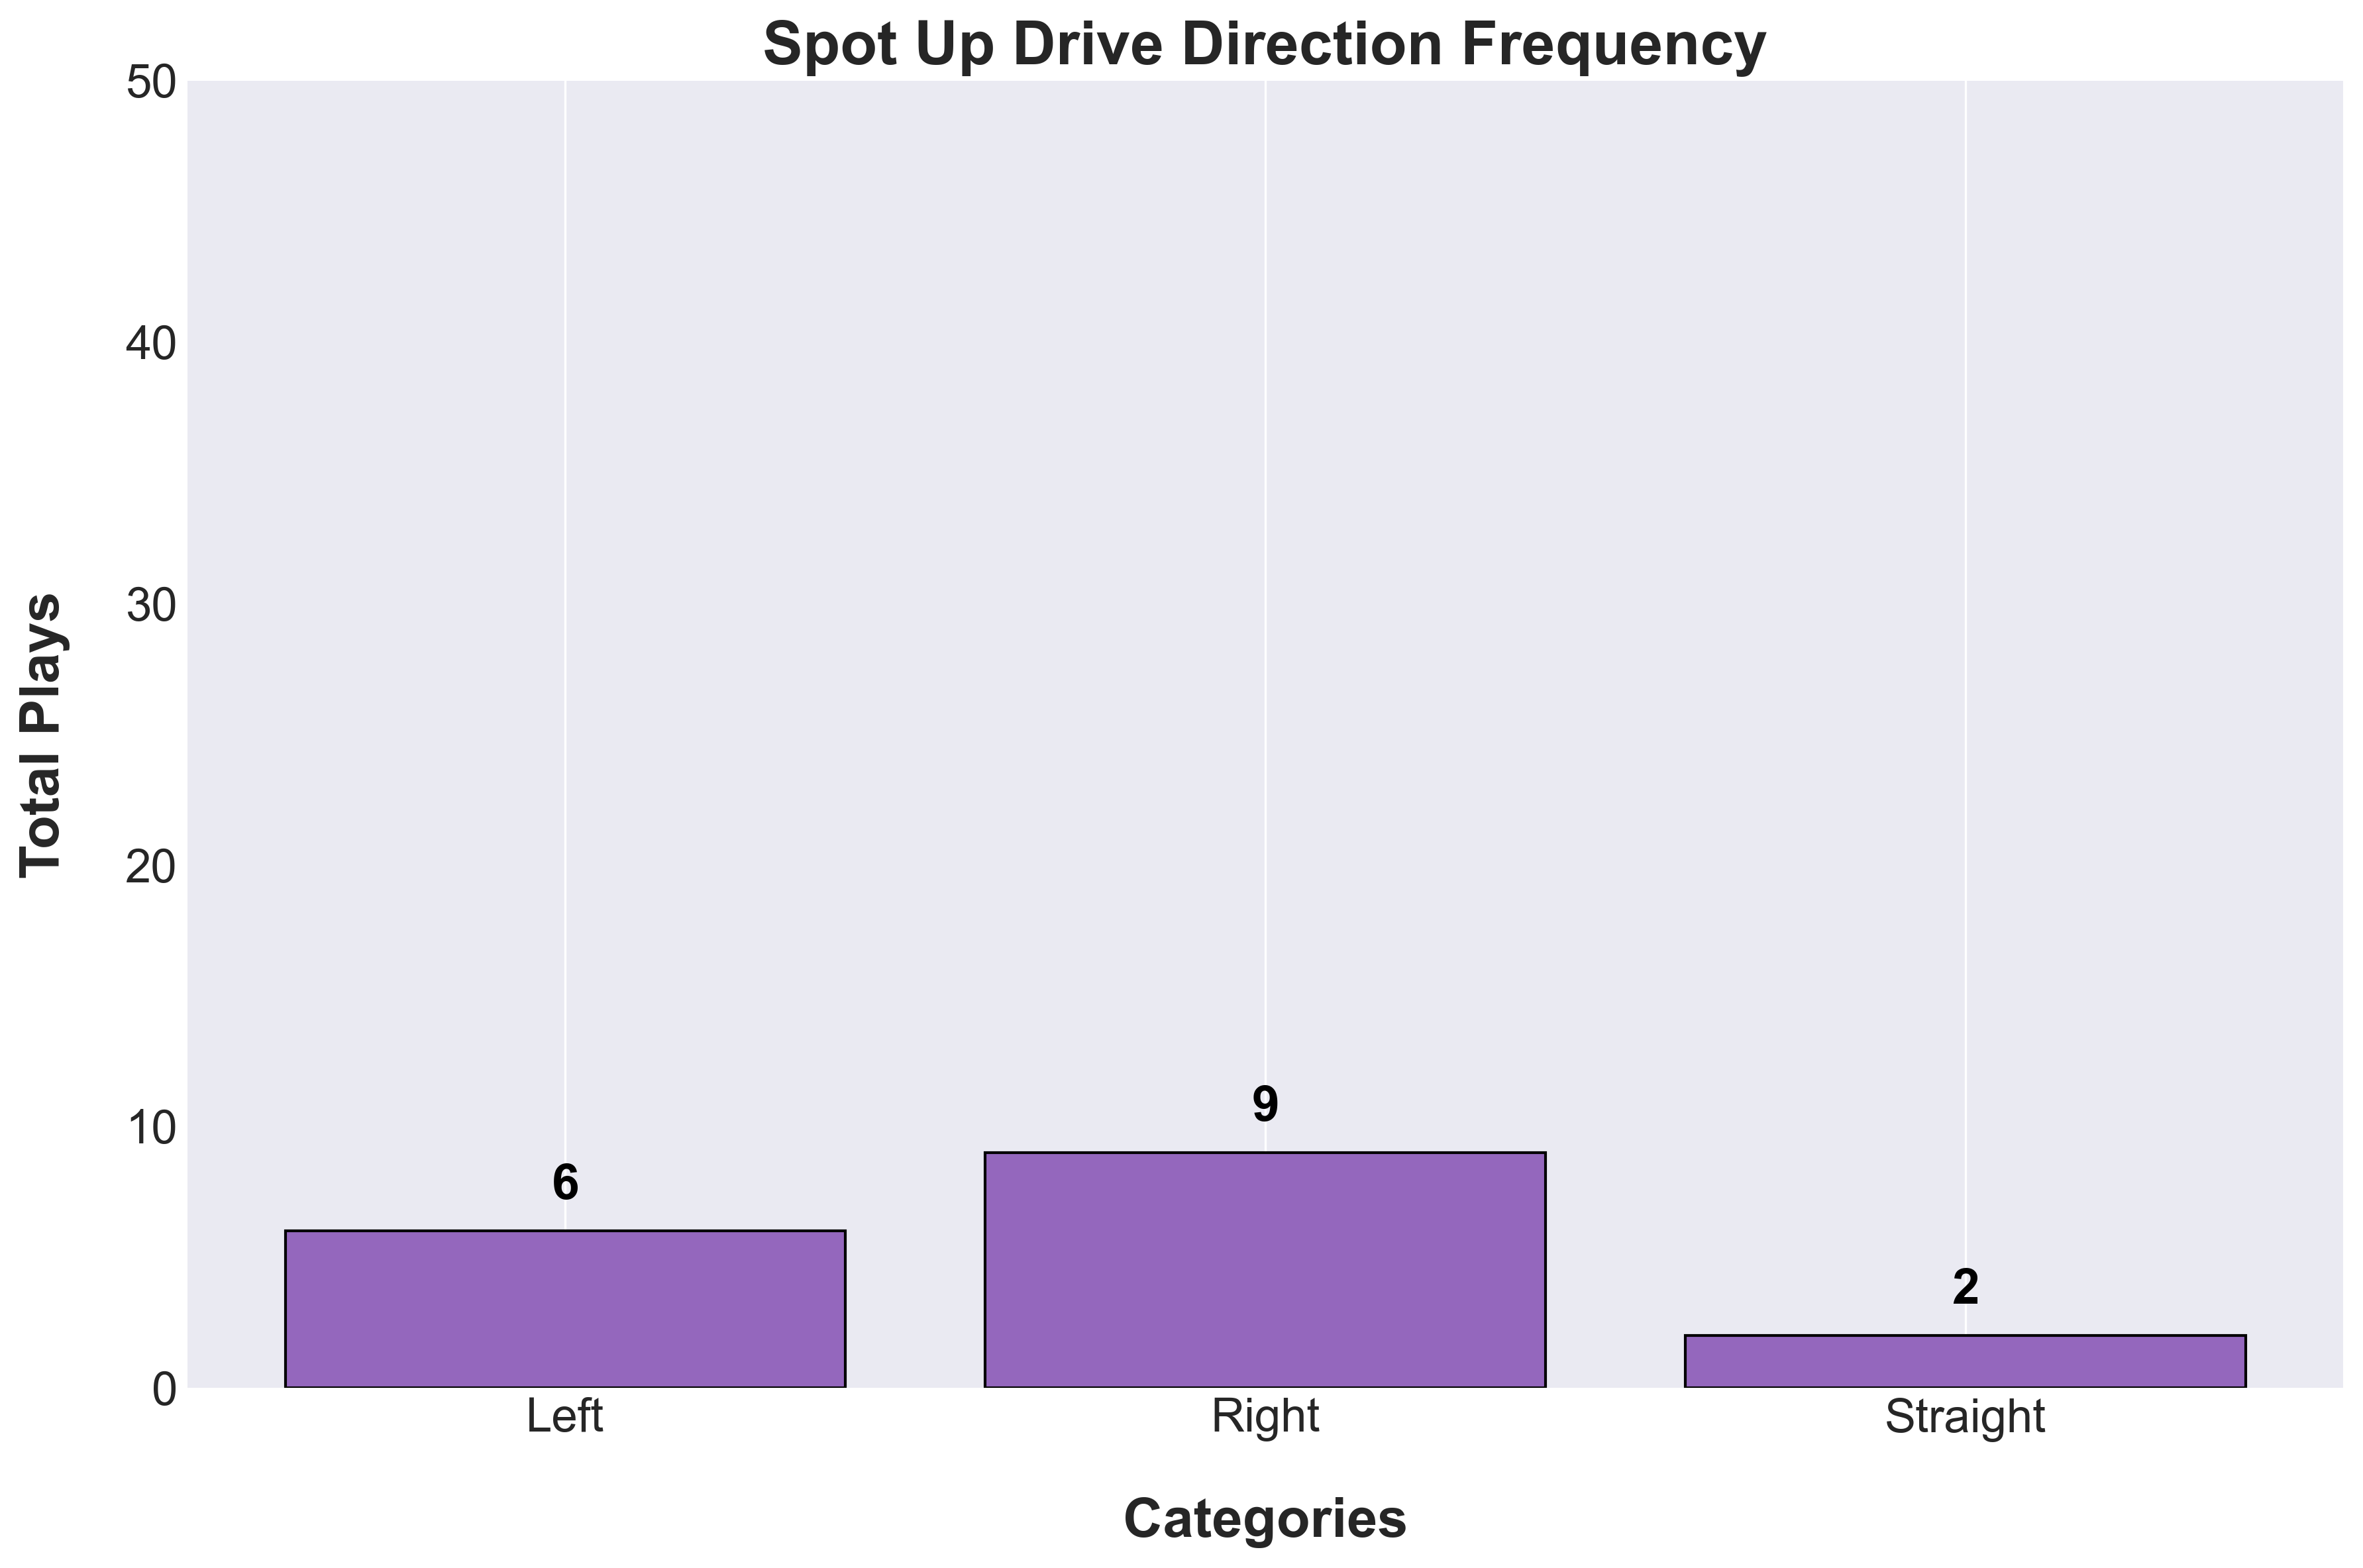
\includegraphics[width=\textwidth, height=.14\textheight]{images/SpotUp_DriveDirection_Freq.png} % Adjust the width of the image to fit
    \end{minipage}
    
\end{table}

\vspace{-1em} % Add vertical space before the line (optional)
\hrule height 1pt width 1\textwidth % Adjust height and width
\vspace{1 em} % Add vertical space after the line (optional)

\subsubsection{Stats on where Player gets Spot Ups from}

% Images of where they receive the ball SU Drives / Shots
\begin{table}[H]
    \centering
    \begin{minipage}[c]{0.45\textwidth} % First image minipage (45% of text width)
        \centering
        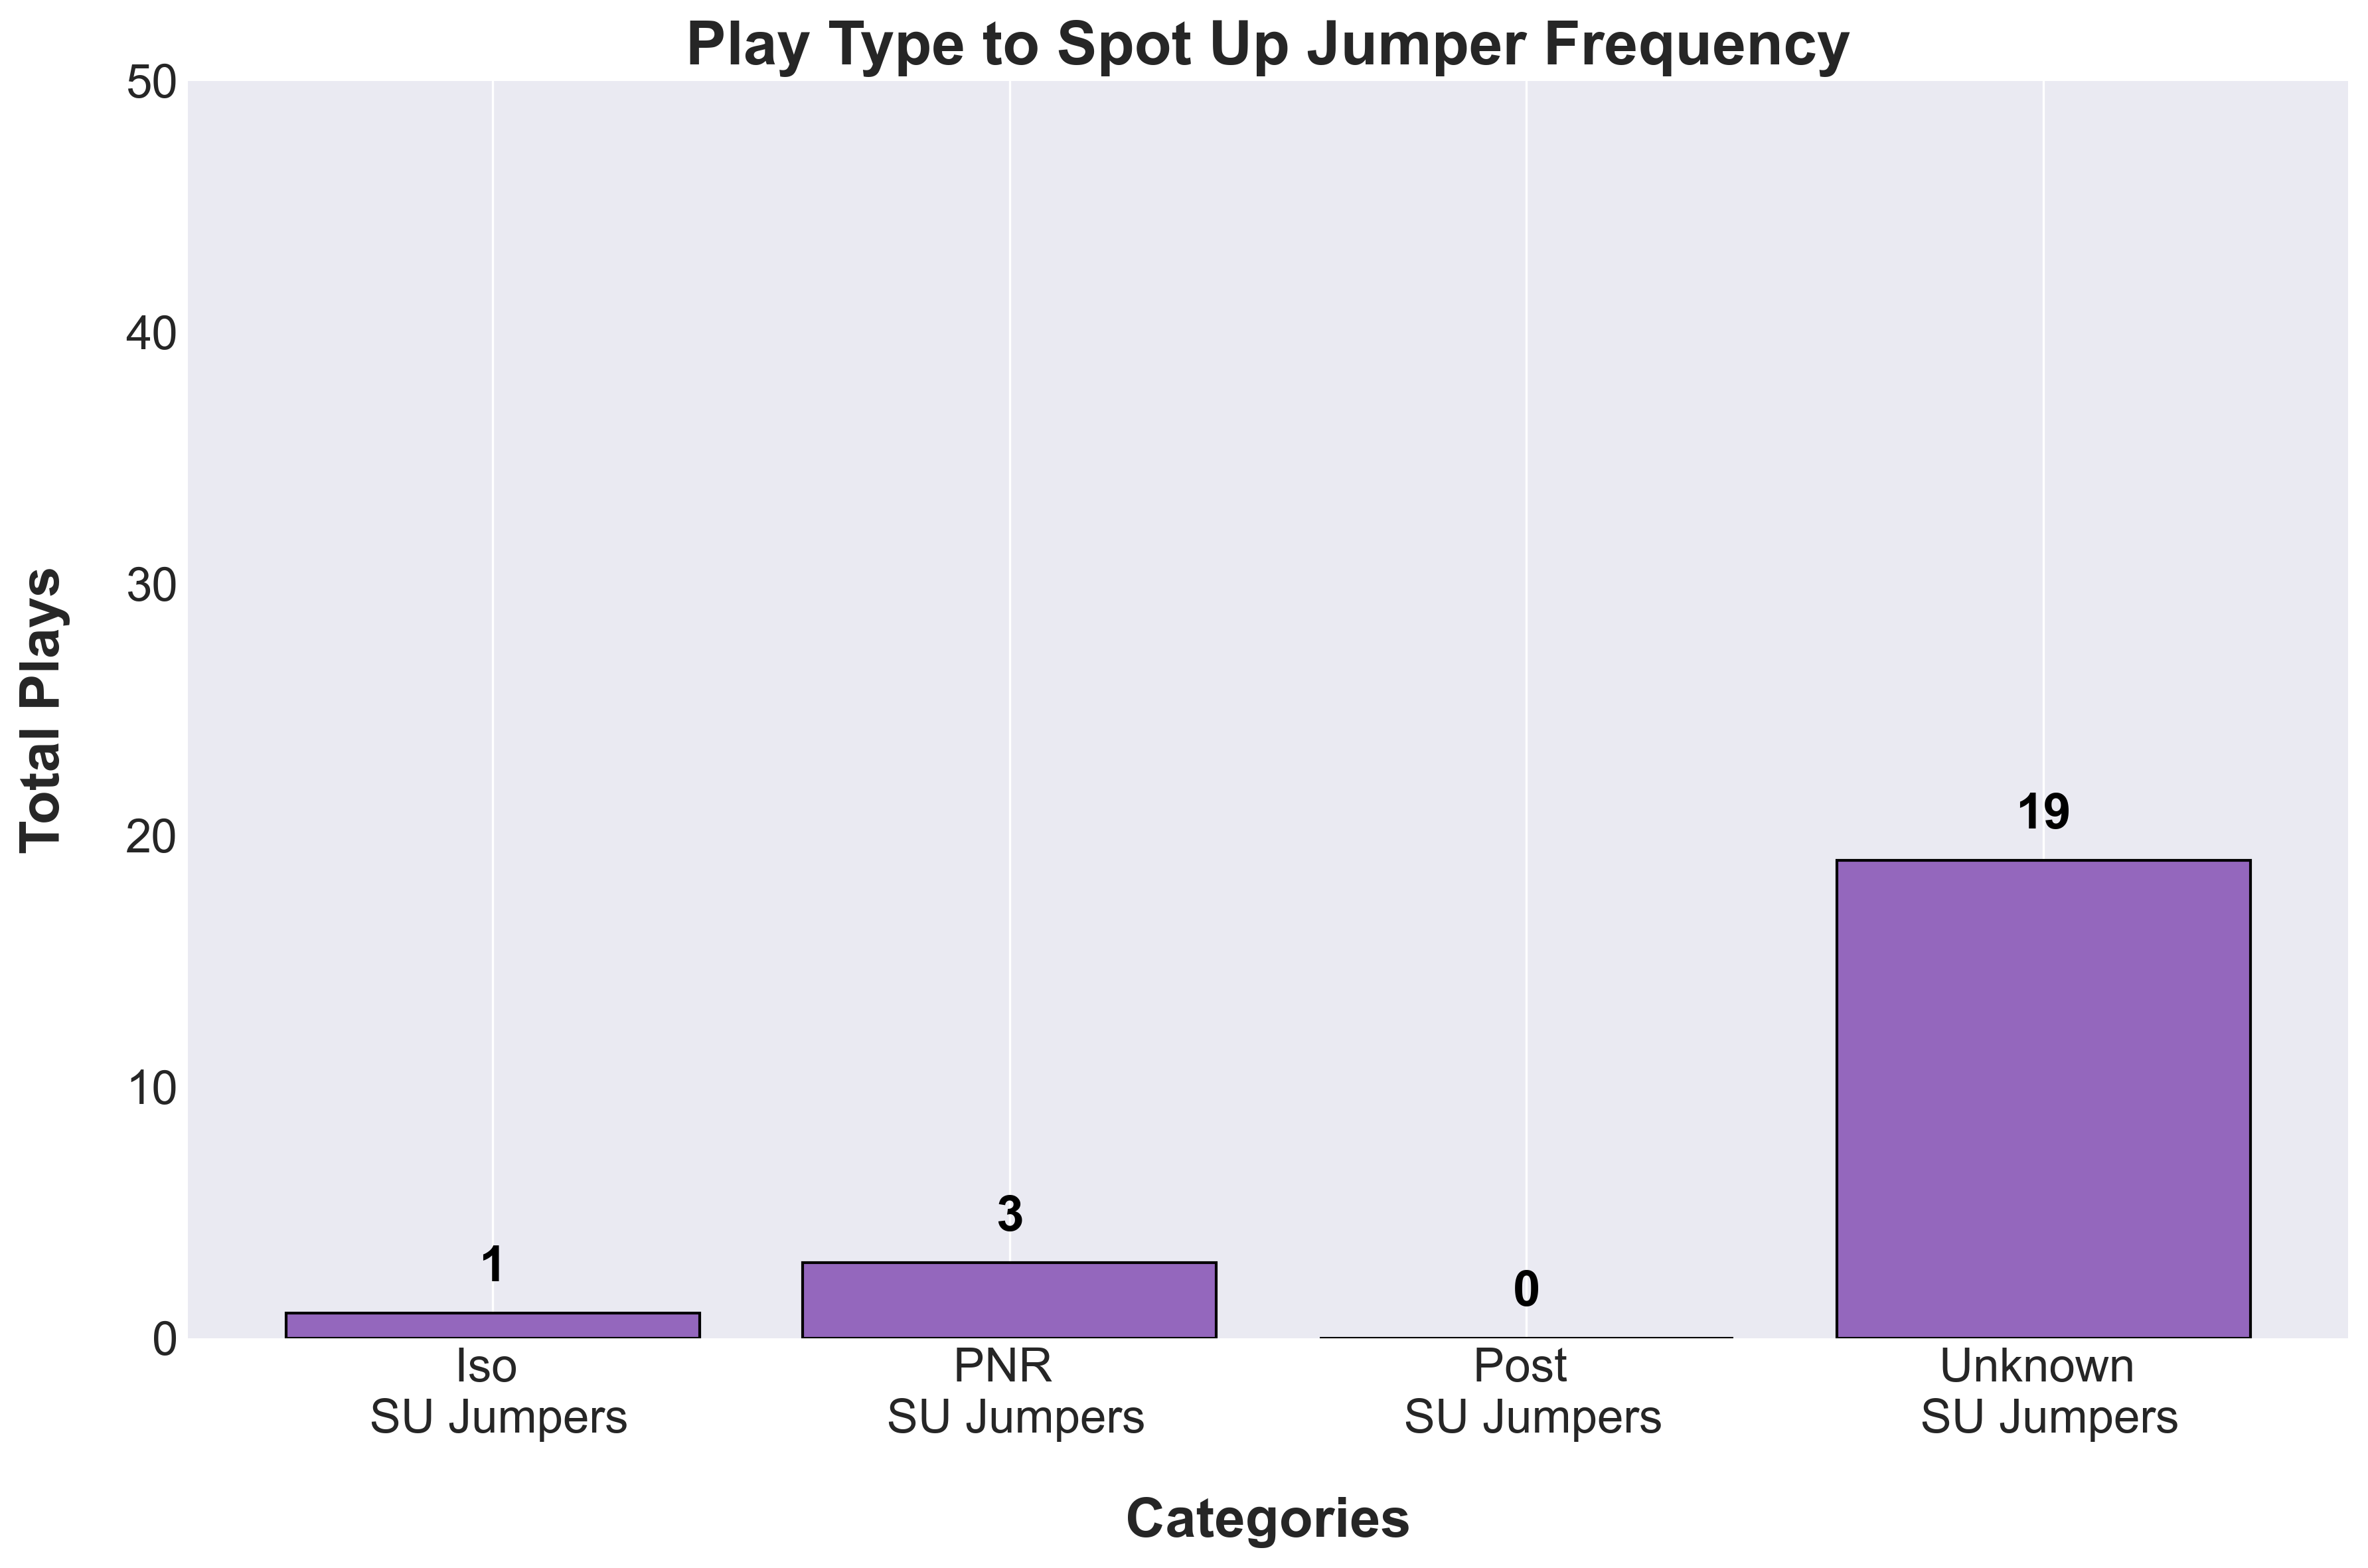
\includegraphics[width=.8\textwidth, height=0.15\textheight]{images/SpotUp_PlayTypeShots_Freq.png} % Adjust image to fill the minipage but scale height to 3/4
    \end{minipage}
    \hfill % Flexible space between images
    \begin{minipage}[c]{0.45\textwidth} % Second image minipage (45% of text width)
        \centering
        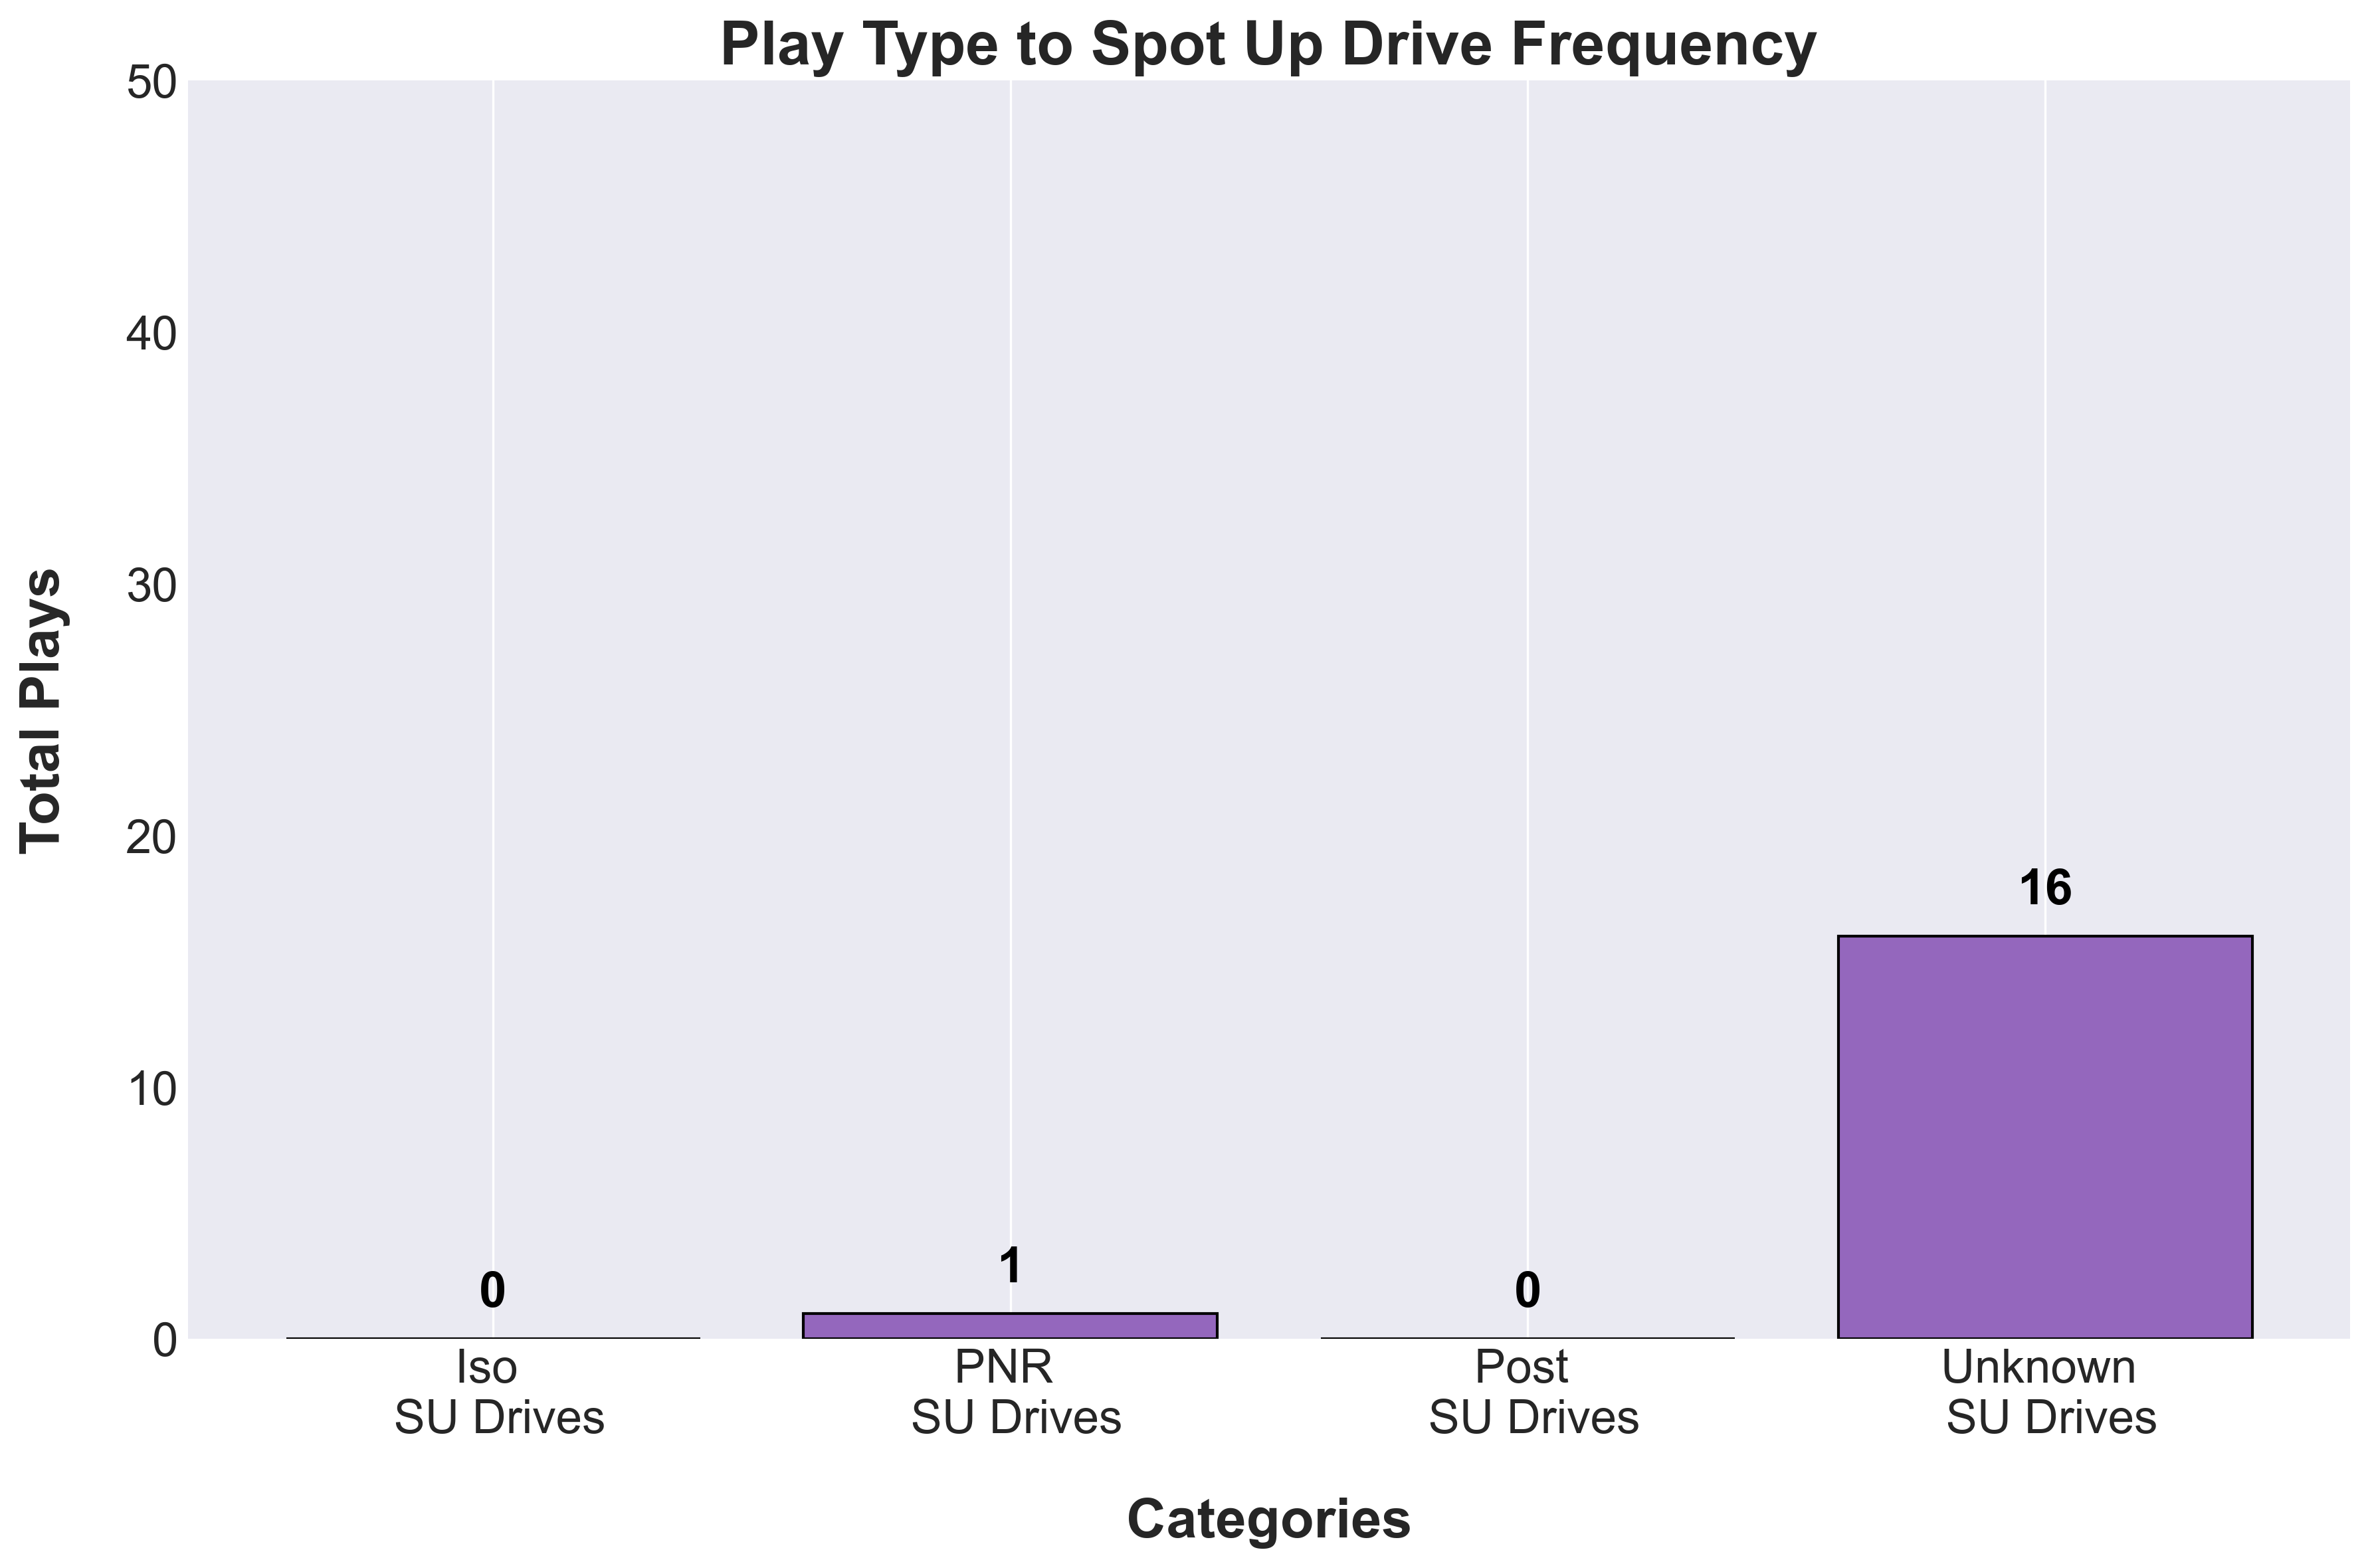
\includegraphics[width=.8\textwidth, height=0.15\textheight]{images/SpotUp_PlayTypeDrives_Freq.png} % Adjust image to fill the minipage but scale height to 3/4
    \end{minipage}
\end{table}

\vspace{-1em} % Add vertical space before the line (optional)
\vspace{-1em} % Add vertical space after the line (optional)

% Tables of where they receive the ball SU Drives / Shots
\begin{table}[H]
    \centering
    \raisebox{-1.5em}{
    \begin{minipage}[t]{0.45\textwidth} % Left table minipage
        \centering
        {\small \text{Different Playtype to Jumpshot Statistics}} % Center the title
        \vskip .25em % Adds vertical space between title and table
        \scalebox{.7}{ % Scale the entire table
            \scriptsize % Reduce the font size
            \renewcommand{\arraystretch}{1.3} % Adjust the number to increase or decrease row spacing
            \begin{tabular}{
            >{\centering\arraybackslash}p{1.25cm} 
            >{\centering\arraybackslash}p{.75cm} 
            >{\centering\arraybackslash}p{.5cm} 
            >{\centering\arraybackslash}p{.5cm}
            >{\centering\arraybackslash}p{.5cm} 
            >{\centering\arraybackslash}p{.5cm} 
            >{\centering\arraybackslash}p{.5cm}
            >{\centering\arraybackslash}p{.75cm}
            >{\centering\arraybackslash}p{.5cm} 
            >{\centering\arraybackslash}p{.5cm}}
            \toprule
            \textbf{PlayType} & \textbf{Plays} & \textbf{3PA} & \textbf{3PM} & \textbf{3P\%}  & \textbf{MiA} & \textbf{MiM} & \textbf{Mi\%}  & \textbf{TO} & \textbf{Foul} \\
            \midrule
            
                
            
                
            
                
            
                
            
                
            
                
                    Iso & 1 & 1 & 0 &
                    0.0 & 
                    0 & 0 &
                    - &
                    0 & 0 \\
                
            
                
            
                
            
                
            
                
                    PNR & 4 & 4 & 2 &
                    33.33 & 
                    0 & 0 &
                    - &
                    0 & 0 \\
                
            
                
            
                
            
                
            
                
            
                
            
                
            
                
            
                
            
                
            
                
            
                
            
                
            



            \bottomrule
        \end{tabular}
        }
    \end{minipage}
    \hfill % Flexible space between the two tables
    \begin{minipage}[t]{0.45\textwidth} % Right table minipage
        \centering
        {\small \text{Different Playtype to Drive Statistics}}% Center the title
        \vskip .25em % Adds vertical space between title and table
        \scalebox{.65}{ % Scale the entire table
            \scriptsize % Reduce the font size
            \renewcommand{\arraystretch}{1.3} % Adjust the number to increase or decrease row spacing
            \begin{tabular}{
            >{\centering\arraybackslash}p{1.25cm} 
            >{\centering\arraybackslash}p{.75cm} 
            >{\centering\arraybackslash}p{.5cm} 
            >{\centering\arraybackslash}p{.5cm}
            >{\centering\arraybackslash}p{.5cm} 
            >{\centering\arraybackslash}p{.5cm} 
            >{\centering\arraybackslash}p{.5cm}
            >{\centering\arraybackslash}p{.75cm}
            >{\centering\arraybackslash}p{.5cm} 
            >{\centering\arraybackslash}p{.5cm}}
            \toprule
            \textbf{PlayType} & \textbf{Plays} & \textbf{2PA} & \textbf{2PM} & \textbf{2P\%} & \textbf{MiA} & \textbf{MiM} & \textbf{Mi\%} & \textbf{TO} & \textbf{Foul} \\
            \midrule
            
                
            
                
            
                
            
                
            
                
            
                
            
                
            
                
                    PNR & 4 &
                    2 & 1 &
                    50.0 &
                    0 & 0 &
                    - &
                    2 & 0 \\
                
            
                
            
                
            
                
            
                
                    Post & 2 &
                    2 & 2 &
                    100.0 &
                    1 & 1 &
                    100.0 &
                    0 & 0 \\
                
            
                
            
                
            
                
            
                
            
                
            
                
            
                
            
                
            
                
            
                
            

            
            \bottomrule
        \end{tabular}
        }
    \end{minipage}
    }
\end{table}

\vspace{1em} % Add vertical space before the line (optional)
\vspace{-1em} % Add vertical space after the line (optional)

% Post -> Jumpshot Stats by Passer
\begin{table}[H]
    \raisebox{3em}{ % Adjust this value to shift the tables vertically
    \begin{minipage}[t]{0.6\textwidth} % Left side (table) takes 85% of the width
        \flushleft
        \centering % Centering the title and the table
        \text{Post - Jumpshot Stats by Passer} % Title above the table in bold
        \vskip .25em % Adds vertical space between title and table
        \scalebox{.6}{ % Scale the entire table down by half
            \renewcommand{\arraystretch}{1.4} % Adjust the number to increase or decrease row spacing
            \begin{tabular}{
            >{\centering\arraybackslash}p{3cm} 
            >{\centering\arraybackslash}p{.75cm} 
            >{\centering\arraybackslash}p{.75cm} 
            >{\centering\arraybackslash}p{.75cm} 
            >{\centering\arraybackslash}p{.75cm}
            >{\centering\arraybackslash}p{.75cm}
            >{\centering\arraybackslash}p{.75cm} 
            >{\centering\arraybackslash}p{.75cm}
            >{\centering\arraybackslash}p{.75cm} 
            >{\centering\arraybackslash}p{.75cm}}% Adjust column widths
            \toprule
            {\scriptsize \textbf{Player}} &
            {\scriptsize \textbf{Plays}} &
            {\scriptsize \textbf{3PA}} &
            {\scriptsize \textbf{3PM}} &
            {\scriptsize \textbf{3P\%}} & 
            {\scriptsize \textbf{MiA}} & 
            {\scriptsize \textbf{MiM}} &
            {\scriptsize \textbf{Mi\%}} &
            {\scriptsize \textbf{TO}} &
            {\scriptsize \textbf{Foul}} \\
            \midrule
            
                
            
                
            
                
            
                
            
                
            
                
            
                
            
                
            
                
            
                
            
                
            
                
            
                
            
                
            
                
                    
                
            
                
            
                
            
                
            
                
            
                
            
                
            
                
            

            \bottomrule
        \end{tabular}
        } % End of \scalebox
    \end{minipage}
    } % End of raisebox, closing the adjustment
    \hfill % This adds some flexible space between the table and the image
    \begin{minipage}[c]{0.35\textwidth} % Right side (image) takes 10% of the width
        \flushright
        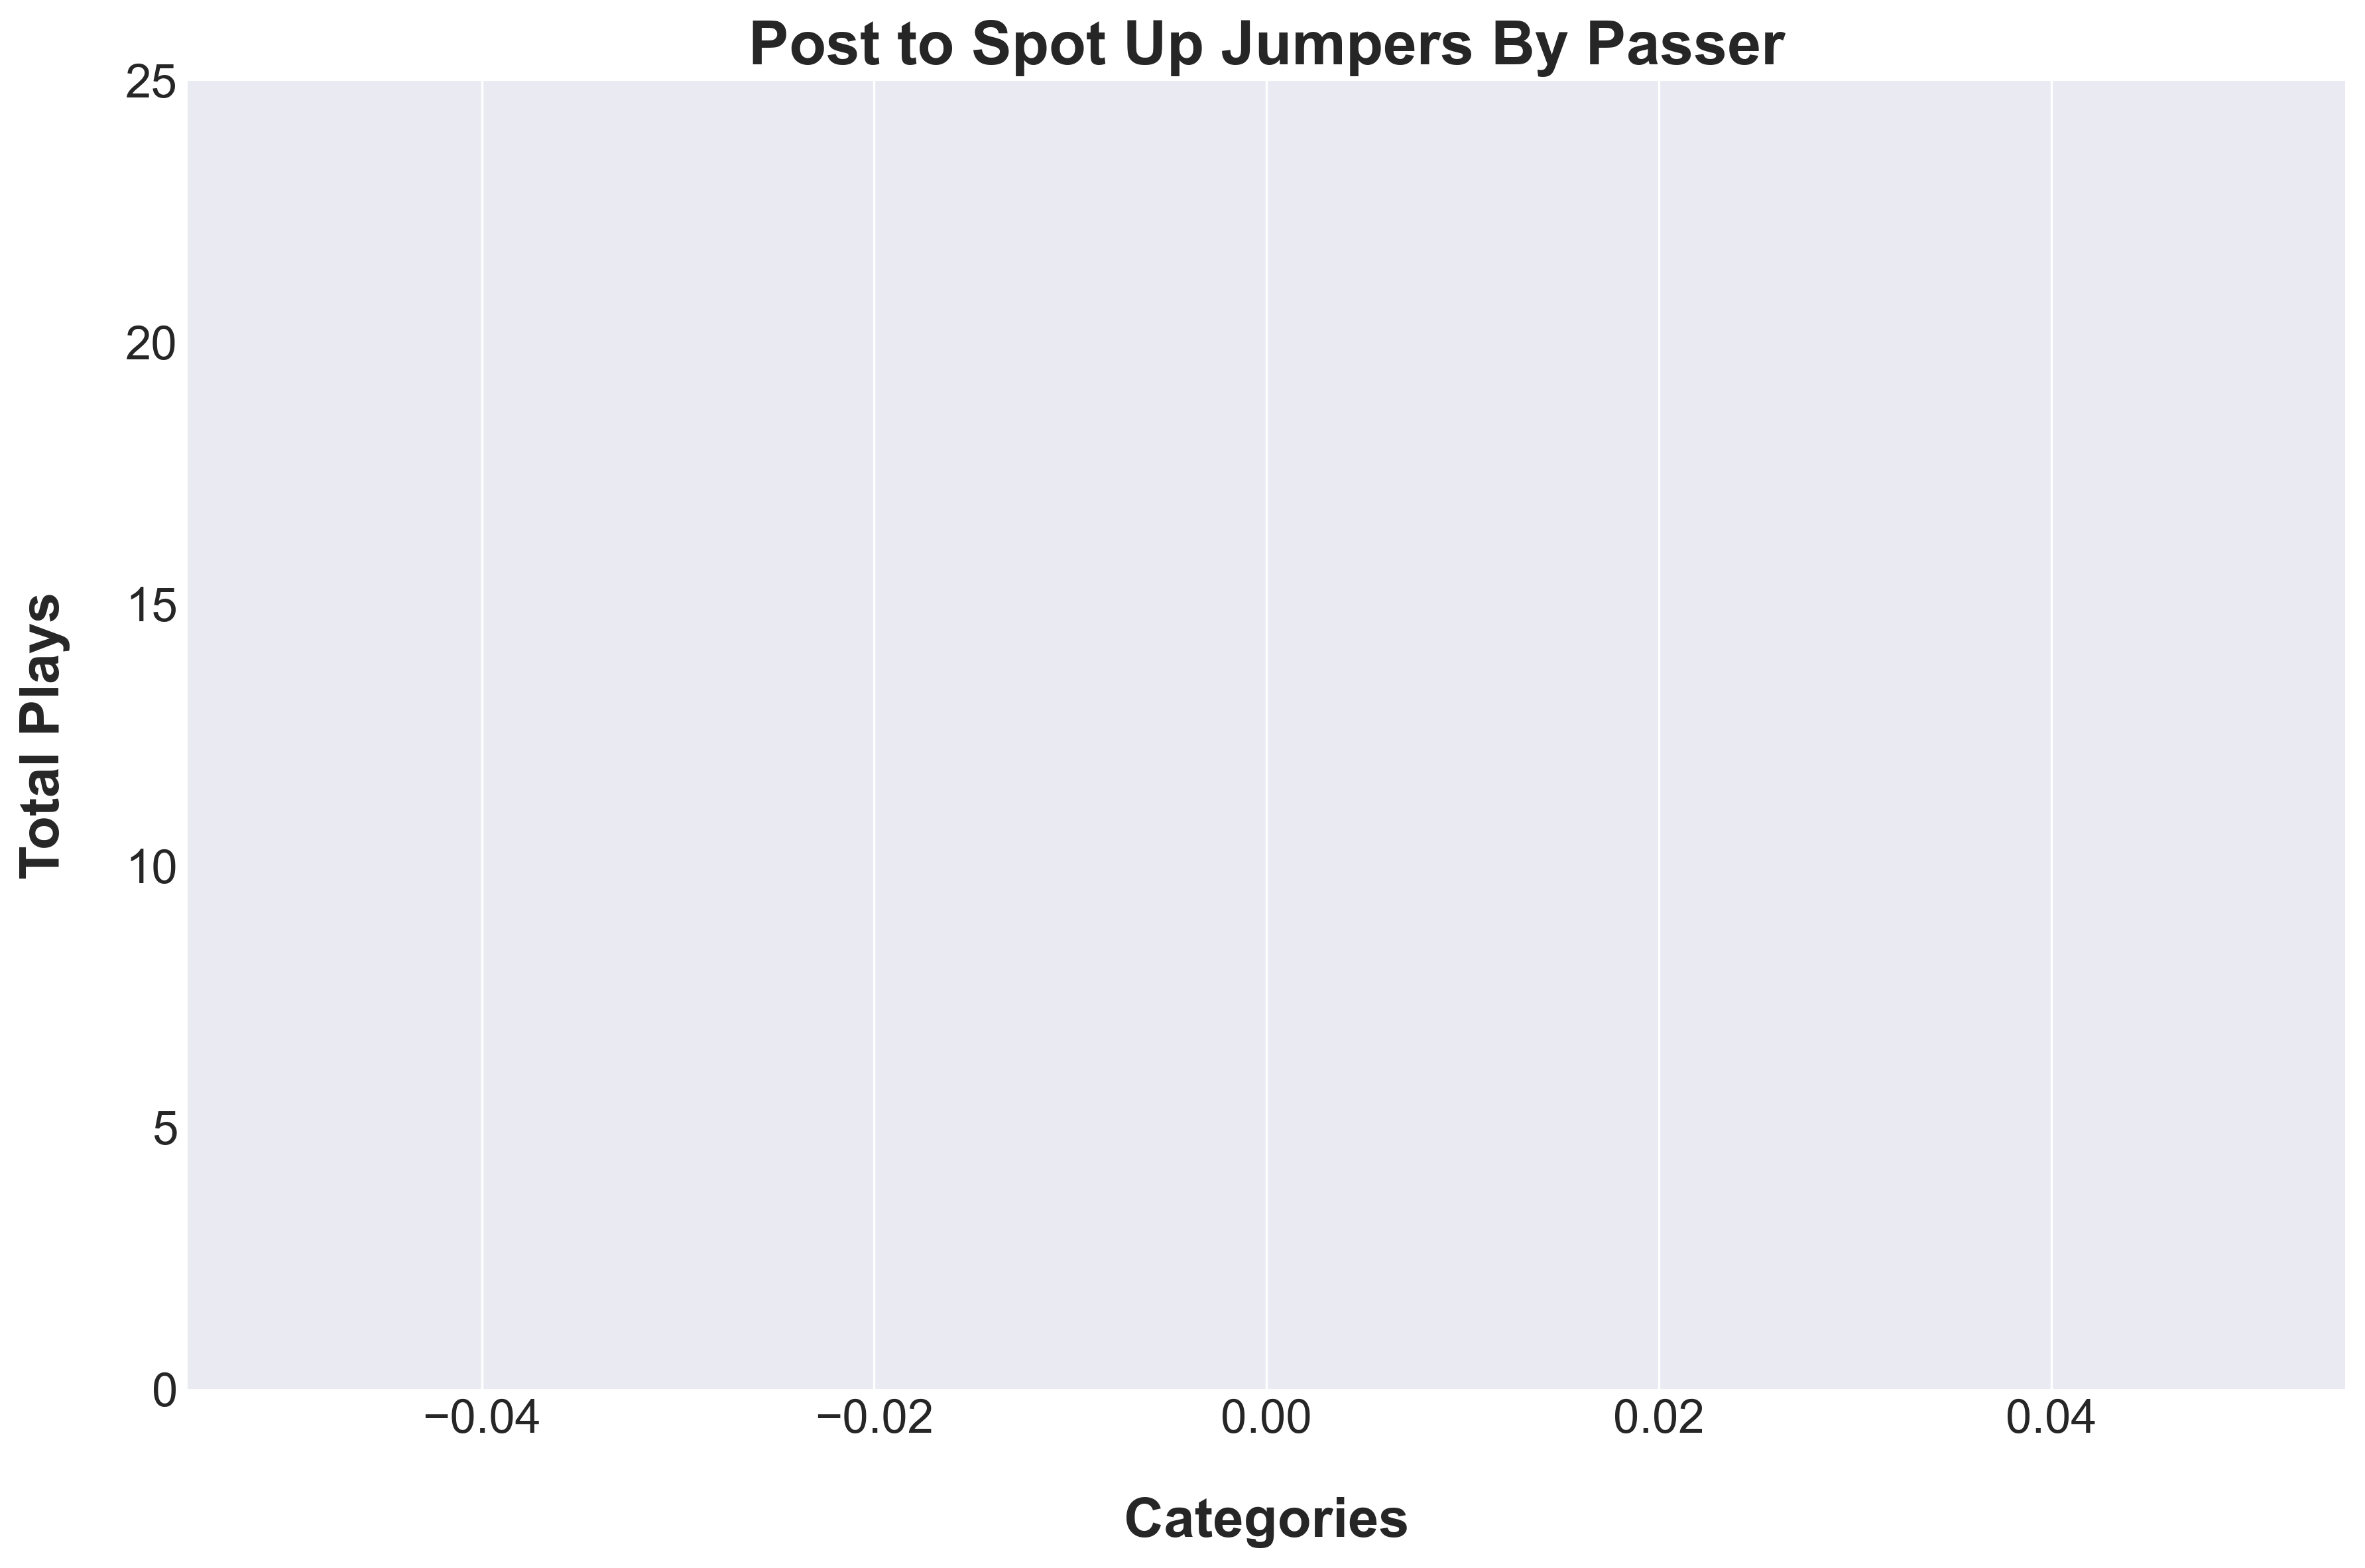
\includegraphics[width=\textwidth, height=.14\textheight]{images/SpotUp_PostShotsPlayer_Freq.png} % Adjust the width of the image to fit
    \end{minipage}
\end{table}

\vspace{-1em} % Add vertical space before the line (optional)
\vspace{-1em} % Add vertical space after the line (optional)

% Iso -> Jumpshot Stats by Passer
\begin{table}[H]
    \raisebox{3em}{ % Adjust this value to shift the tables vertically
    \begin{minipage}[t]{0.6\textwidth} % Left side (table) takes 85% of the width
        \flushleft
        \centering % Centering the title and the table
        \text{Iso - Jumpshot Stats by Passer} % Title above the table in bold
        \vskip .25em % Adds vertical space between title and table
        \scalebox{.6}{ % Scale the entire table down by half
            \renewcommand{\arraystretch}{1.4} % Adjust the number to increase or decrease row spacing
            \begin{tabular}{
            >{\centering\arraybackslash}p{3cm} 
            >{\centering\arraybackslash}p{.75cm} 
            >{\centering\arraybackslash}p{.75cm} 
            >{\centering\arraybackslash}p{.75cm} 
            >{\centering\arraybackslash}p{.75cm}
            >{\centering\arraybackslash}p{.75cm}
            >{\centering\arraybackslash}p{.75cm} 
            >{\centering\arraybackslash}p{.75cm}
            >{\centering\arraybackslash}p{.75cm}
            >{\centering\arraybackslash}p{.75cm}}% Adjust column widths
            \toprule
            {\scriptsize \textbf{Player}} &
            {\scriptsize \textbf{Plays}} &
            {\scriptsize \textbf{3PA}} &
            {\scriptsize \textbf{3PM}} &
            {\scriptsize \textbf{3P\%}} & 
            {\scriptsize \textbf{MiA}} & 
            {\scriptsize \textbf{MiM}} &
            {\scriptsize \textbf{Mi\%}} &
            {\scriptsize \textbf{TO}} &
            {\scriptsize \textbf{Foul}} \\
            \midrule
            
                
            
                
            
                
            
                
            
                
            
                
            
                
                    
                        Brock Bowen & 
                        1 & 
                        1 & 
                        0 & 
                        0.0 & 
                        0 & 
                        0 & 
                        - & 
                        0 & 
                        0 \\
                    
                
            
                
            
                
            
                
            
                
            
                
            
                
            
                
            
                
            
                
            
                
            
                
            
                
            
                
            
                
            
                
            
            \bottomrule
        \end{tabular}
        } % End of \scalebox
    \end{minipage}
    } % End of raisebox, closing the adjustment
    \hfill % This adds some flexible space between the table and the image
    \begin{minipage}[c]{0.35\textwidth} % Right side (image) takes 10% of the width
        \flushright
        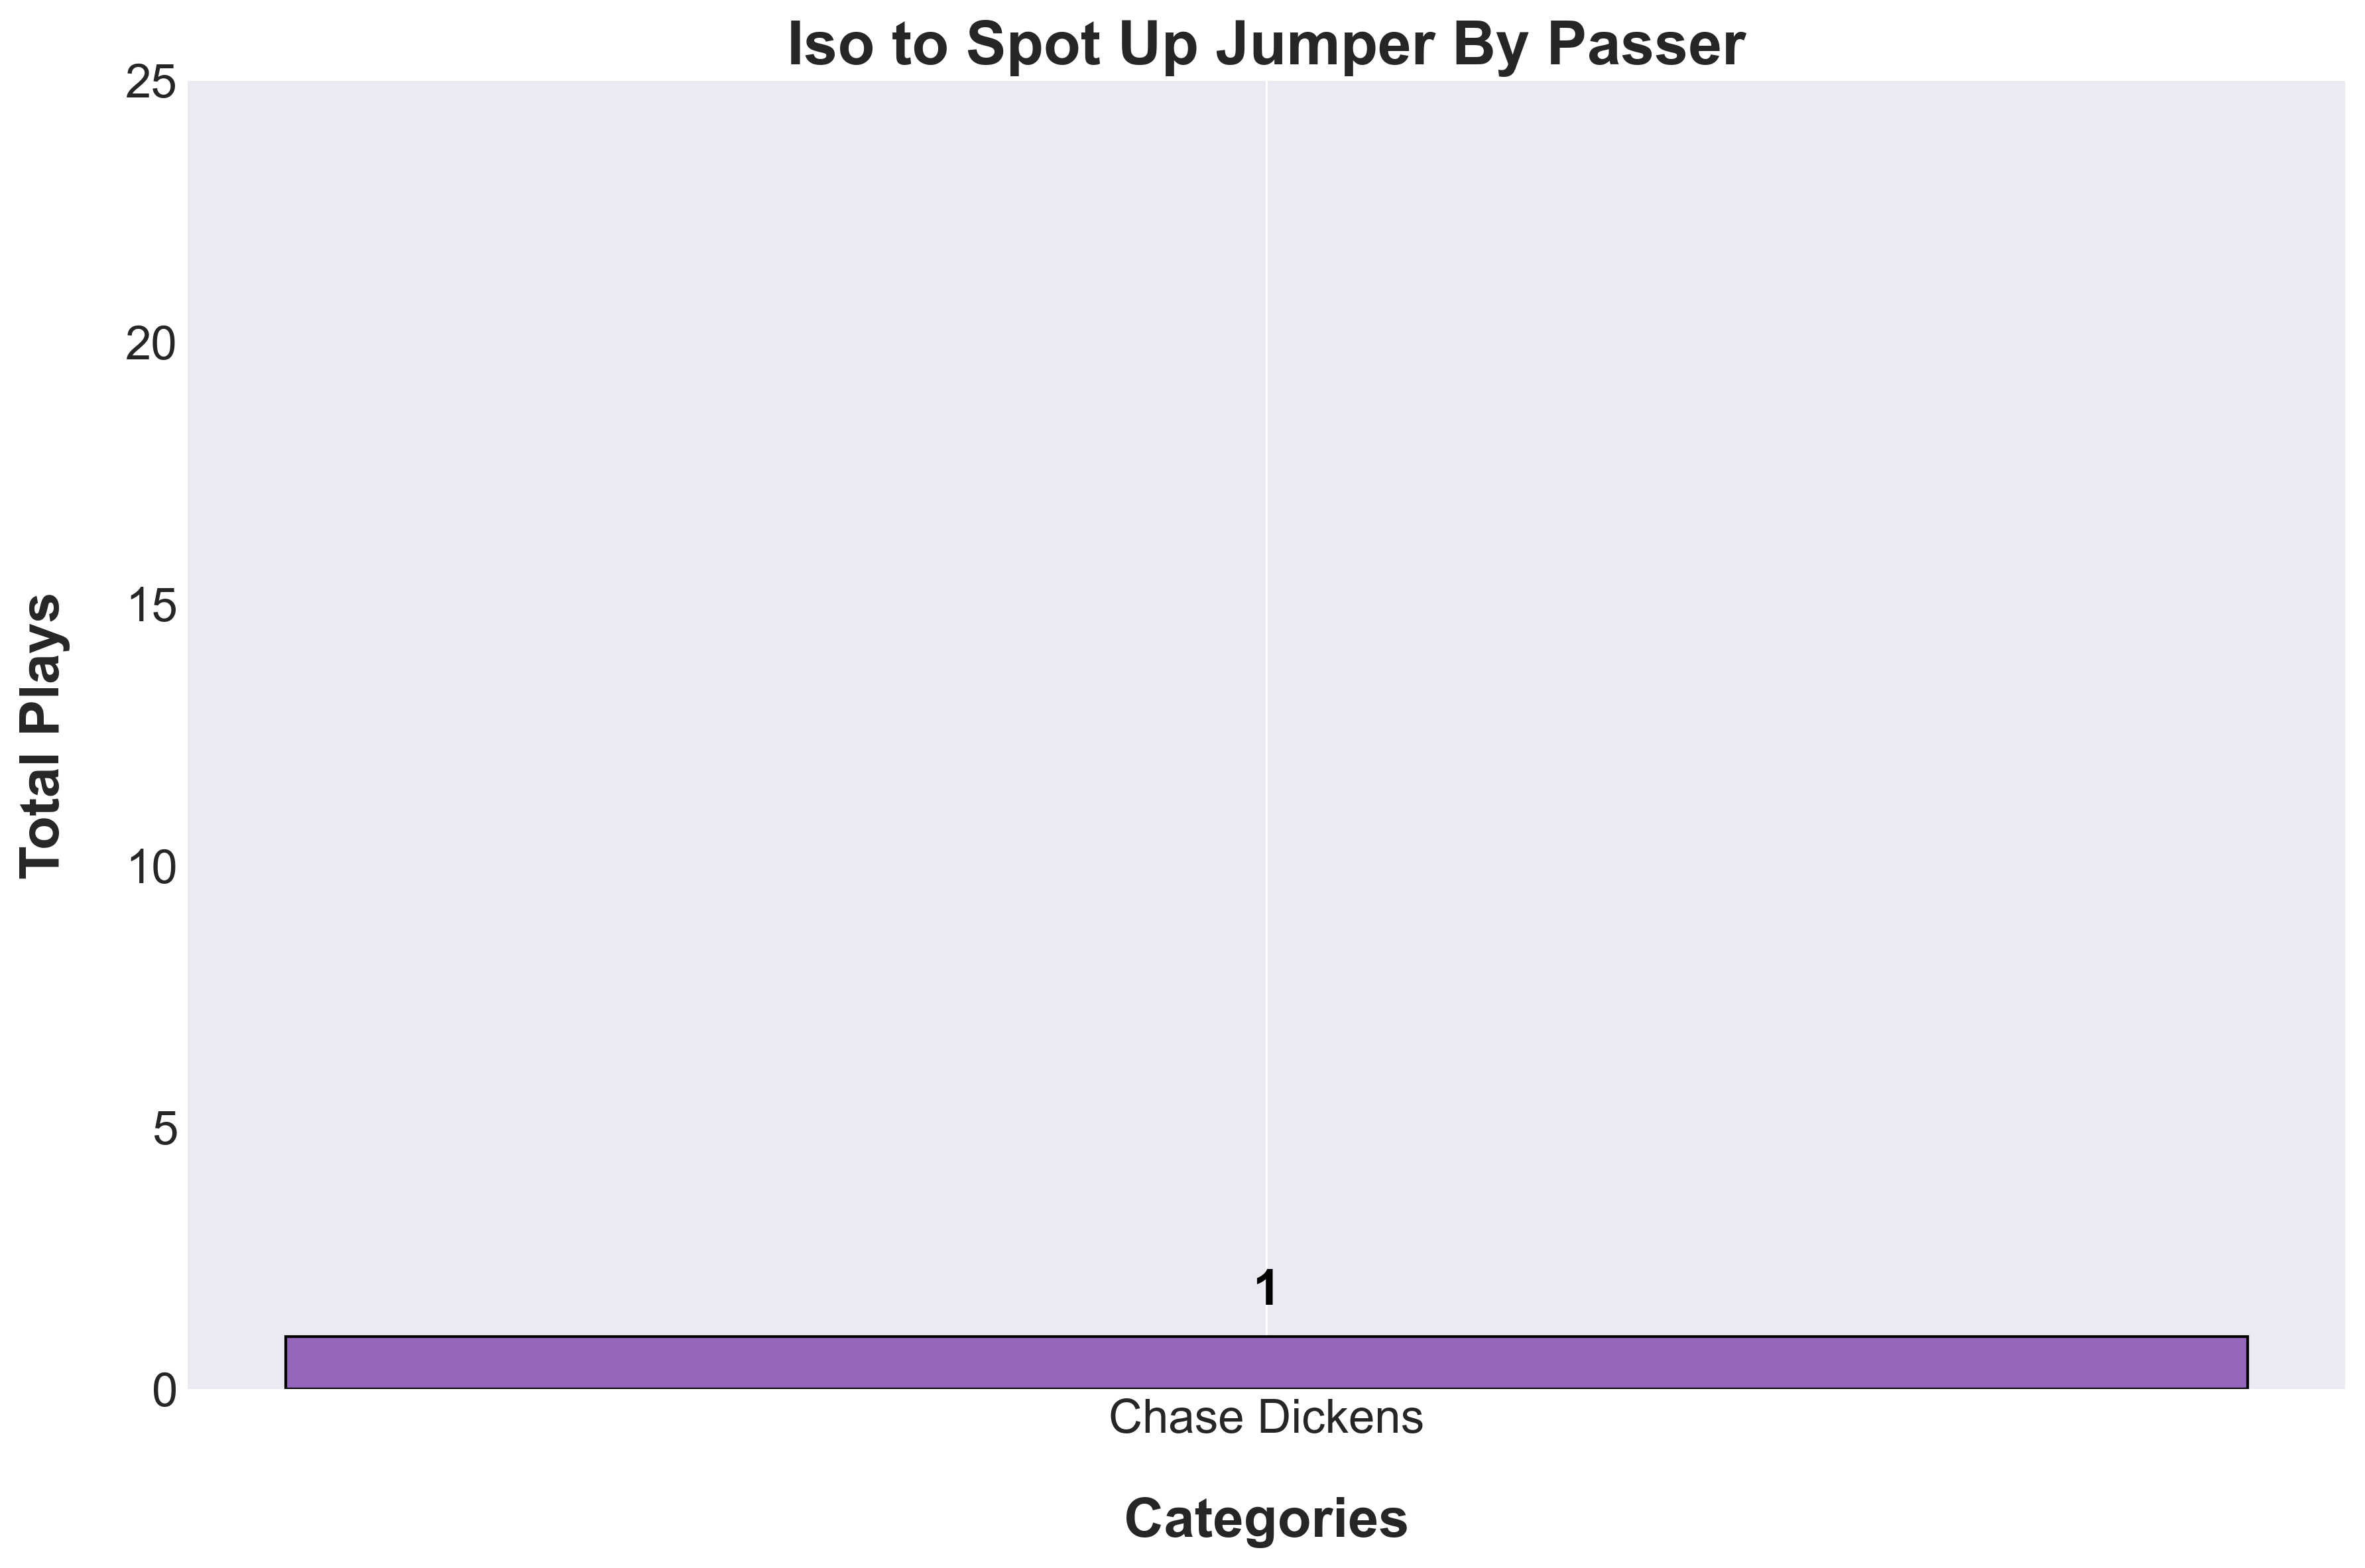
\includegraphics[width=\textwidth, height=.14\textheight]{images/SpotUp_IsoShotsPlayer_Freq.png} % Adjust the width of the image to fit
    \end{minipage}
\end{table}

\vspace{-1em} % Add vertical space before the line (optional)
\vspace{-1em} % Add vertical space after the line (optional)

% PNR -> Jumpshot Stats by Passer
\begin{table}[H]
    \raisebox{3em}{ % Adjust this value to shift the tables vertically
    \begin{minipage}[t]{0.6\textwidth} % Left side (table) takes 85% of the width
        \flushleft
        \centering % Centering the title and the table
        \text{PNR - Jumpshot Stats by Passer} % Title above the table in bold
        \vskip .25em % Adds vertical space between title and table
        \scalebox{.6}{ % Scale the entire table down by half
            \renewcommand{\arraystretch}{1.4} % Adjust the number to increase or decrease row spacing
            \begin{tabular}{
            >{\centering\arraybackslash}p{3cm} 
            >{\centering\arraybackslash}p{.75cm} 
            >{\centering\arraybackslash}p{.75cm} 
            >{\centering\arraybackslash}p{.75cm} 
            >{\centering\arraybackslash}p{.75cm} 
            >{\centering\arraybackslash}p{.75cm}
            >{\centering\arraybackslash}p{.75cm} 
            >{\centering\arraybackslash}p{.75cm}
            >{\centering\arraybackslash}p{.75cm} 
            >{\centering\arraybackslash}p{.75cm}}% Adjust column widths
            \toprule
            {\scriptsize \textbf{Player}} &
            {\scriptsize \textbf{Plays}} &
            {\scriptsize \textbf{3PA}} &
            {\scriptsize \textbf{3PM}} &
            {\scriptsize \textbf{3P\%}} & 
            {\scriptsize \textbf{MiA}} & 
            {\scriptsize \textbf{MiM}} &
            {\scriptsize \textbf{Mi\%}} &
            {\scriptsize \textbf{TO}} &
            {\scriptsize \textbf{Foul}} \\
            \midrule
            
                
            
                
            
                
            
                
            
                
            
                
            
                
            
                
            
                
            
                
            
                
                    
                        Brock Bowen & 
                        3 & 
                        3 & 
                        2 & 
                        66.67 & 
                        0 & 
                        0 & 
                        - & 
                        0 & 
                        0 \\
                    
                        Chase Dickens & 
                        1 & 
                        1 & 
                        0 & 
                        0.0 & 
                        0 & 
                        0 & 
                        - & 
                        0 & 
                        0 \\
                    
                
            
                
            
                
            
                
            
                
            
                
            
                
            
                
            
                
            
                
            
                
            
                
            

            \bottomrule
        \end{tabular}
        } % End of \scalebox
    \end{minipage}
    } % End of raisebox, closing the adjustment
    \hfill % This adds some flexible space between the table and the image
    \begin{minipage}[c]{0.35\textwidth} % Right side (image) takes 10% of the width
        \flushright
        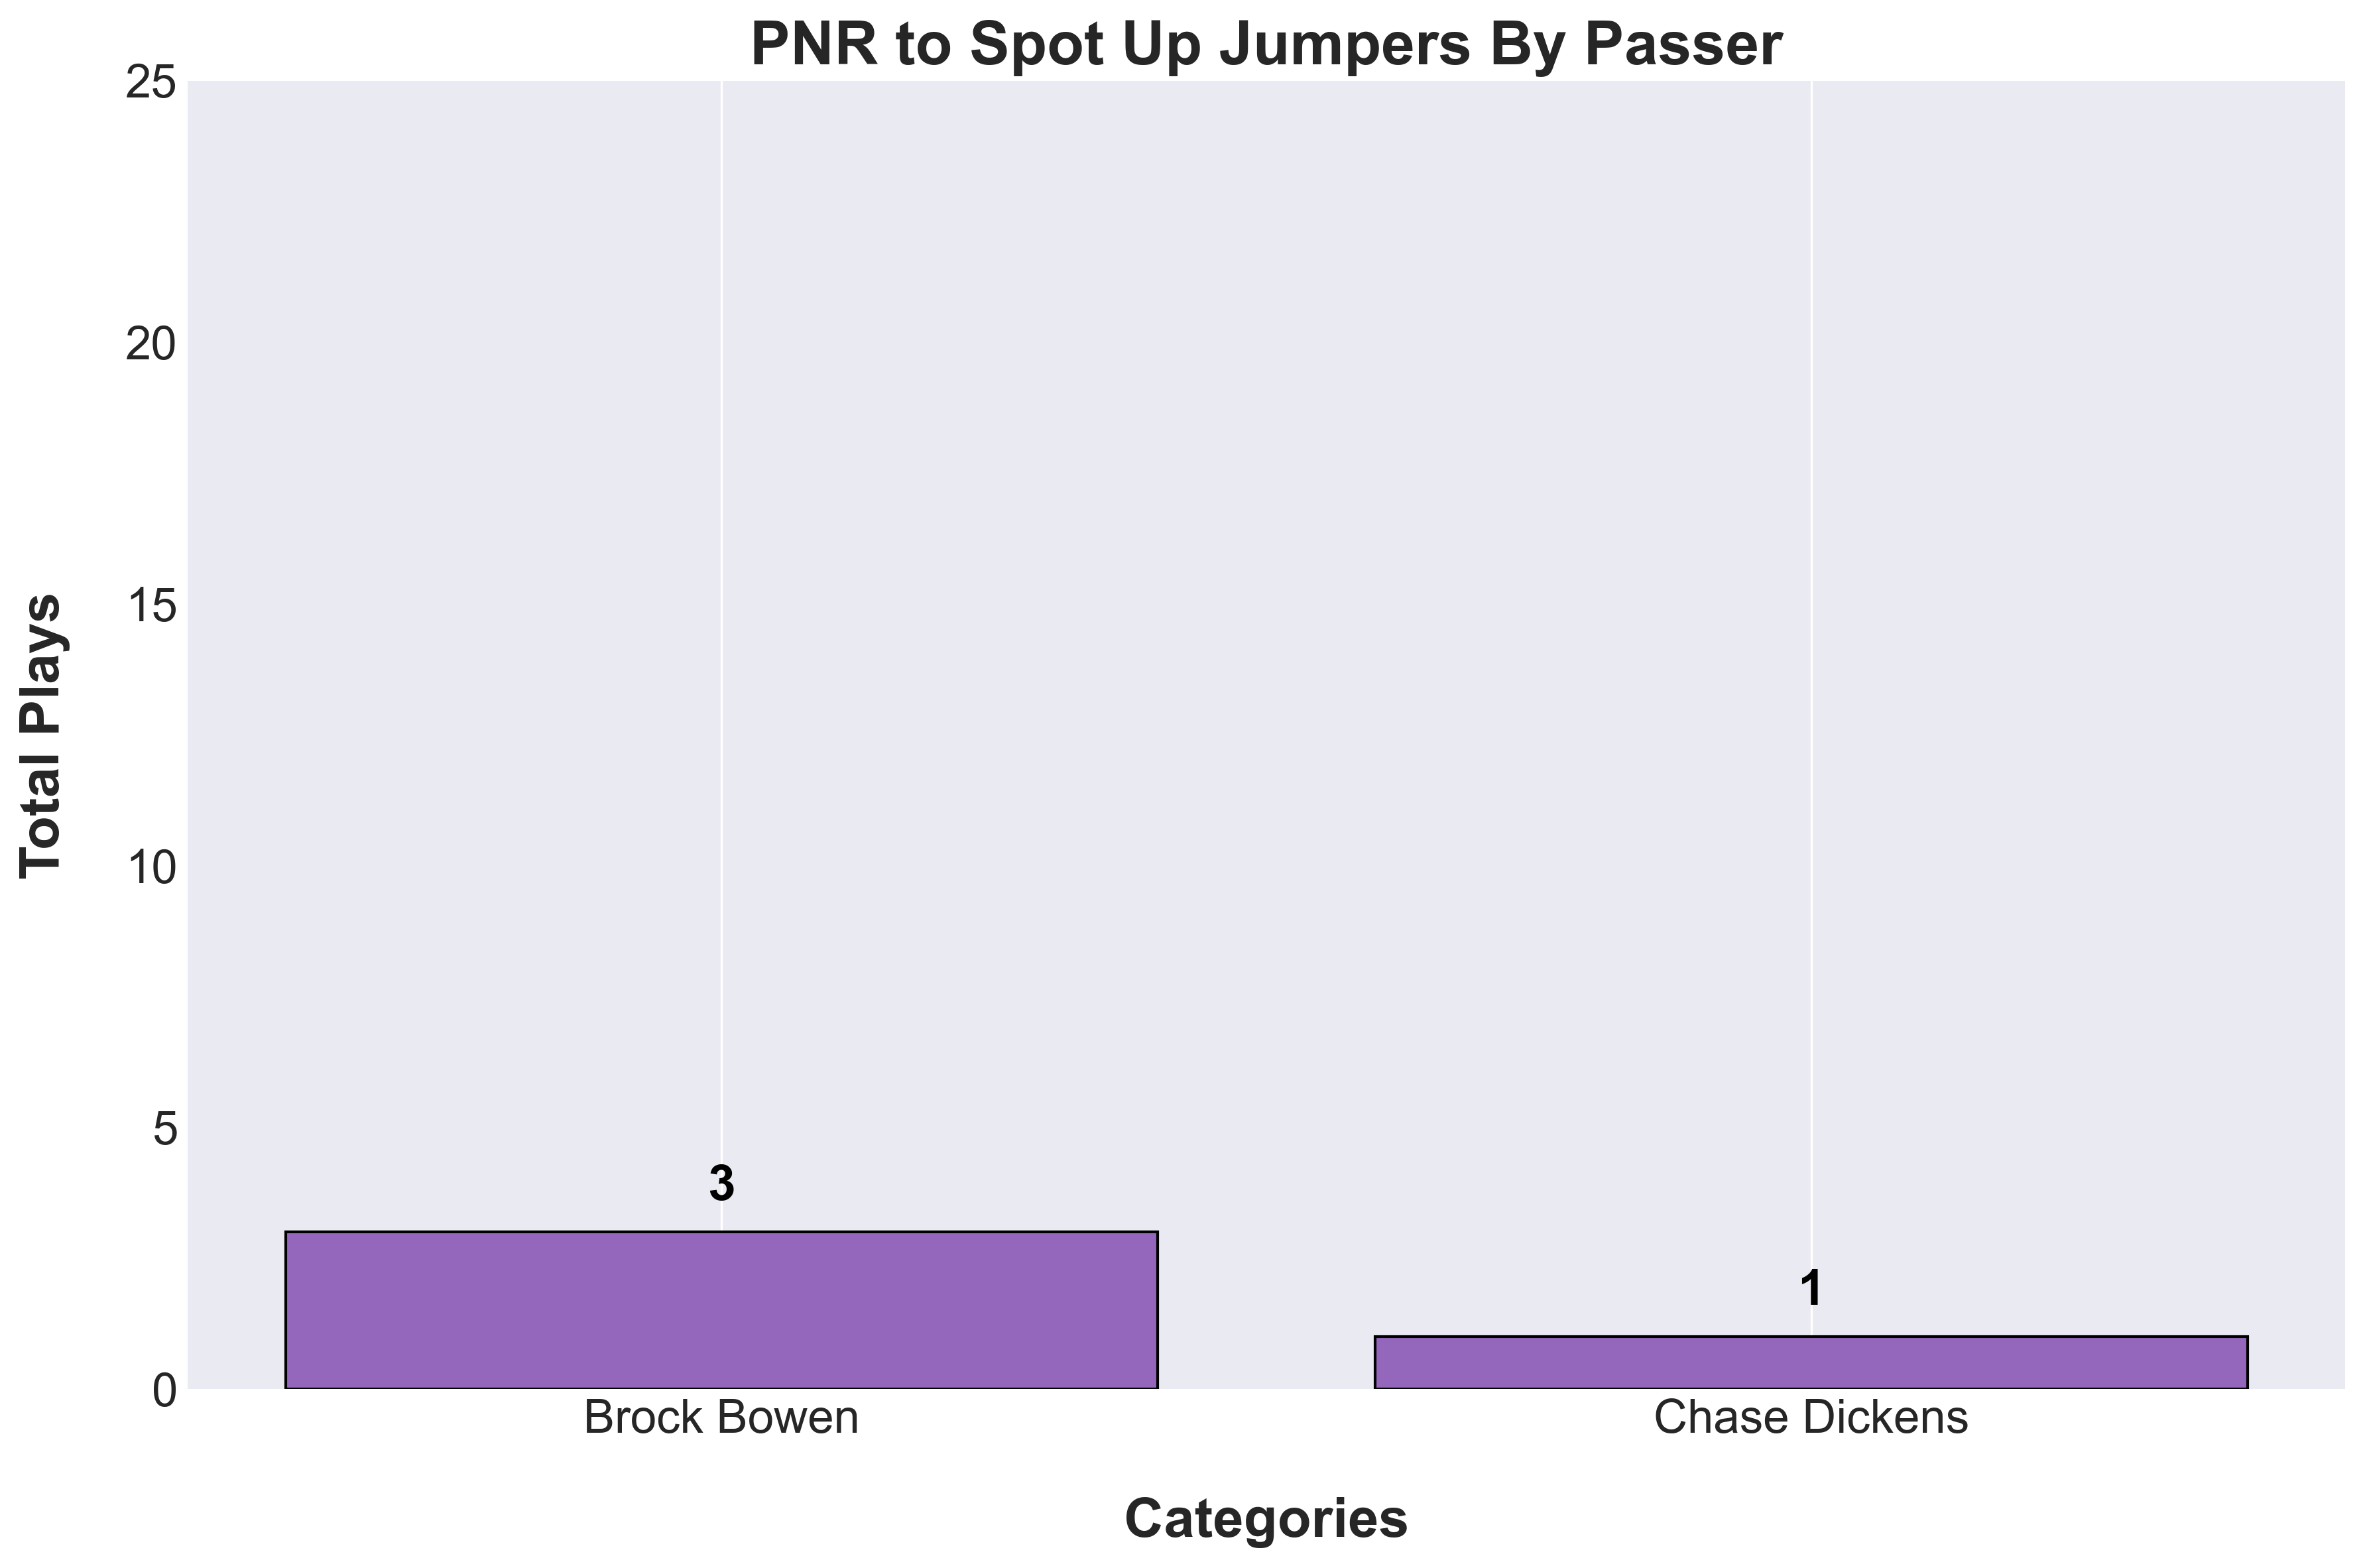
\includegraphics[width=\textwidth, height=.14\textheight]{images/SpotUp_PNRShotsPlayer_Freq.png} % Adjust the width of the image to fit
    \end{minipage}
\end{table}

\vspace{-1em} % Add vertical space before the line (optional)
\vspace{-1em} % Add vertical space after the line (optional)

% Post -> Drive Stats by Passer
\begin{table}[H]
    \raisebox{3em}{ % Adjust this value to shift the tables vertically
    \begin{minipage}[t]{0.6\textwidth} % Left side (table) takes 85% of the width
        \flushleft
        \centering % Centering the title and the table
        \text{Post - Drive Stats by Passer} % Title above the table in bold
        \vskip .25em % Adds vertical space between title and table
        \scalebox{.55}{ % Scale the entire table down by half
            \renewcommand{\arraystretch}{1.4} % Adjust the number to increase or decrease row spacing
            \begin{tabular}{
            >{\centering\arraybackslash}p{3cm} 
            >{\centering\arraybackslash}p{.75cm} 
            >{\centering\arraybackslash}p{.75cm} 
            >{\centering\arraybackslash}p{.75cm} 
            >{\centering\arraybackslash}p{.75cm}
            >{\centering\arraybackslash}p{.75cm} 
            >{\centering\arraybackslash}p{.75cm} 
            >{\centering\arraybackslash}p{.75cm} 
            >{\centering\arraybackslash}p{.75cm}
            >{\centering\arraybackslash}p{.75cm} 
            >{\centering\arraybackslash}p{.75cm}
            >{\centering\arraybackslash}p{.75cm} 
            >{\centering\arraybackslash}p{.75cm}}% Adjust column widths
            \toprule
            {\scriptsize \textbf{Player}} &
            {\scriptsize \textbf{Plays}} &
            {\scriptsize \textbf{3PA}} &
            {\scriptsize \textbf{3PM}} &
            {\scriptsize \textbf{3P\%}} & 
            {\scriptsize \textbf{2PA}} & 
            {\scriptsize \textbf{2PM}} & 
            {\scriptsize \textbf{2P\%}} & 
            {\scriptsize \textbf{MiA}} & 
            {\scriptsize \textbf{MiM}} &
            {\scriptsize \textbf{Mi\%}} &
            {\scriptsize \textbf{TO}} &
            {\scriptsize \textbf{Foul}} \\
            \midrule
            
                
            
                
            
                
            
                
            
                
            
                
            
                
            
                
            
                
            
                
            
                
            
                
            
                
                    
                        Josiah Turner & 
                        1 & 
                        0 & 
                        0 & 
                        - & 
                        1 & 
                        1 & 
                        100.0 & 
                        1 & 
                        1 & 
                        100.0 & 
                        0 & 
                        0 \\
                    
                        Kenny Wilburn & 
                        1 & 
                        0 & 
                        0 & 
                        - & 
                        1 & 
                        1 & 
                        100.0 & 
                        0 & 
                        0 & 
                        - & 
                        0 & 
                        0 \\
                    
                
            
                
            
                
            
                
            
                
            
                
            
                
            
                
            
                
            
                
            

            \bottomrule
        \end{tabular}
        } % End of \scalebox
    \end{minipage}
    } % End of raisebox, closing the adjustment
    \hfill % This adds some flexible space between the table and the image
    \begin{minipage}[c]{0.35\textwidth} % Right side (image) takes 10% of the width
        \flushright
        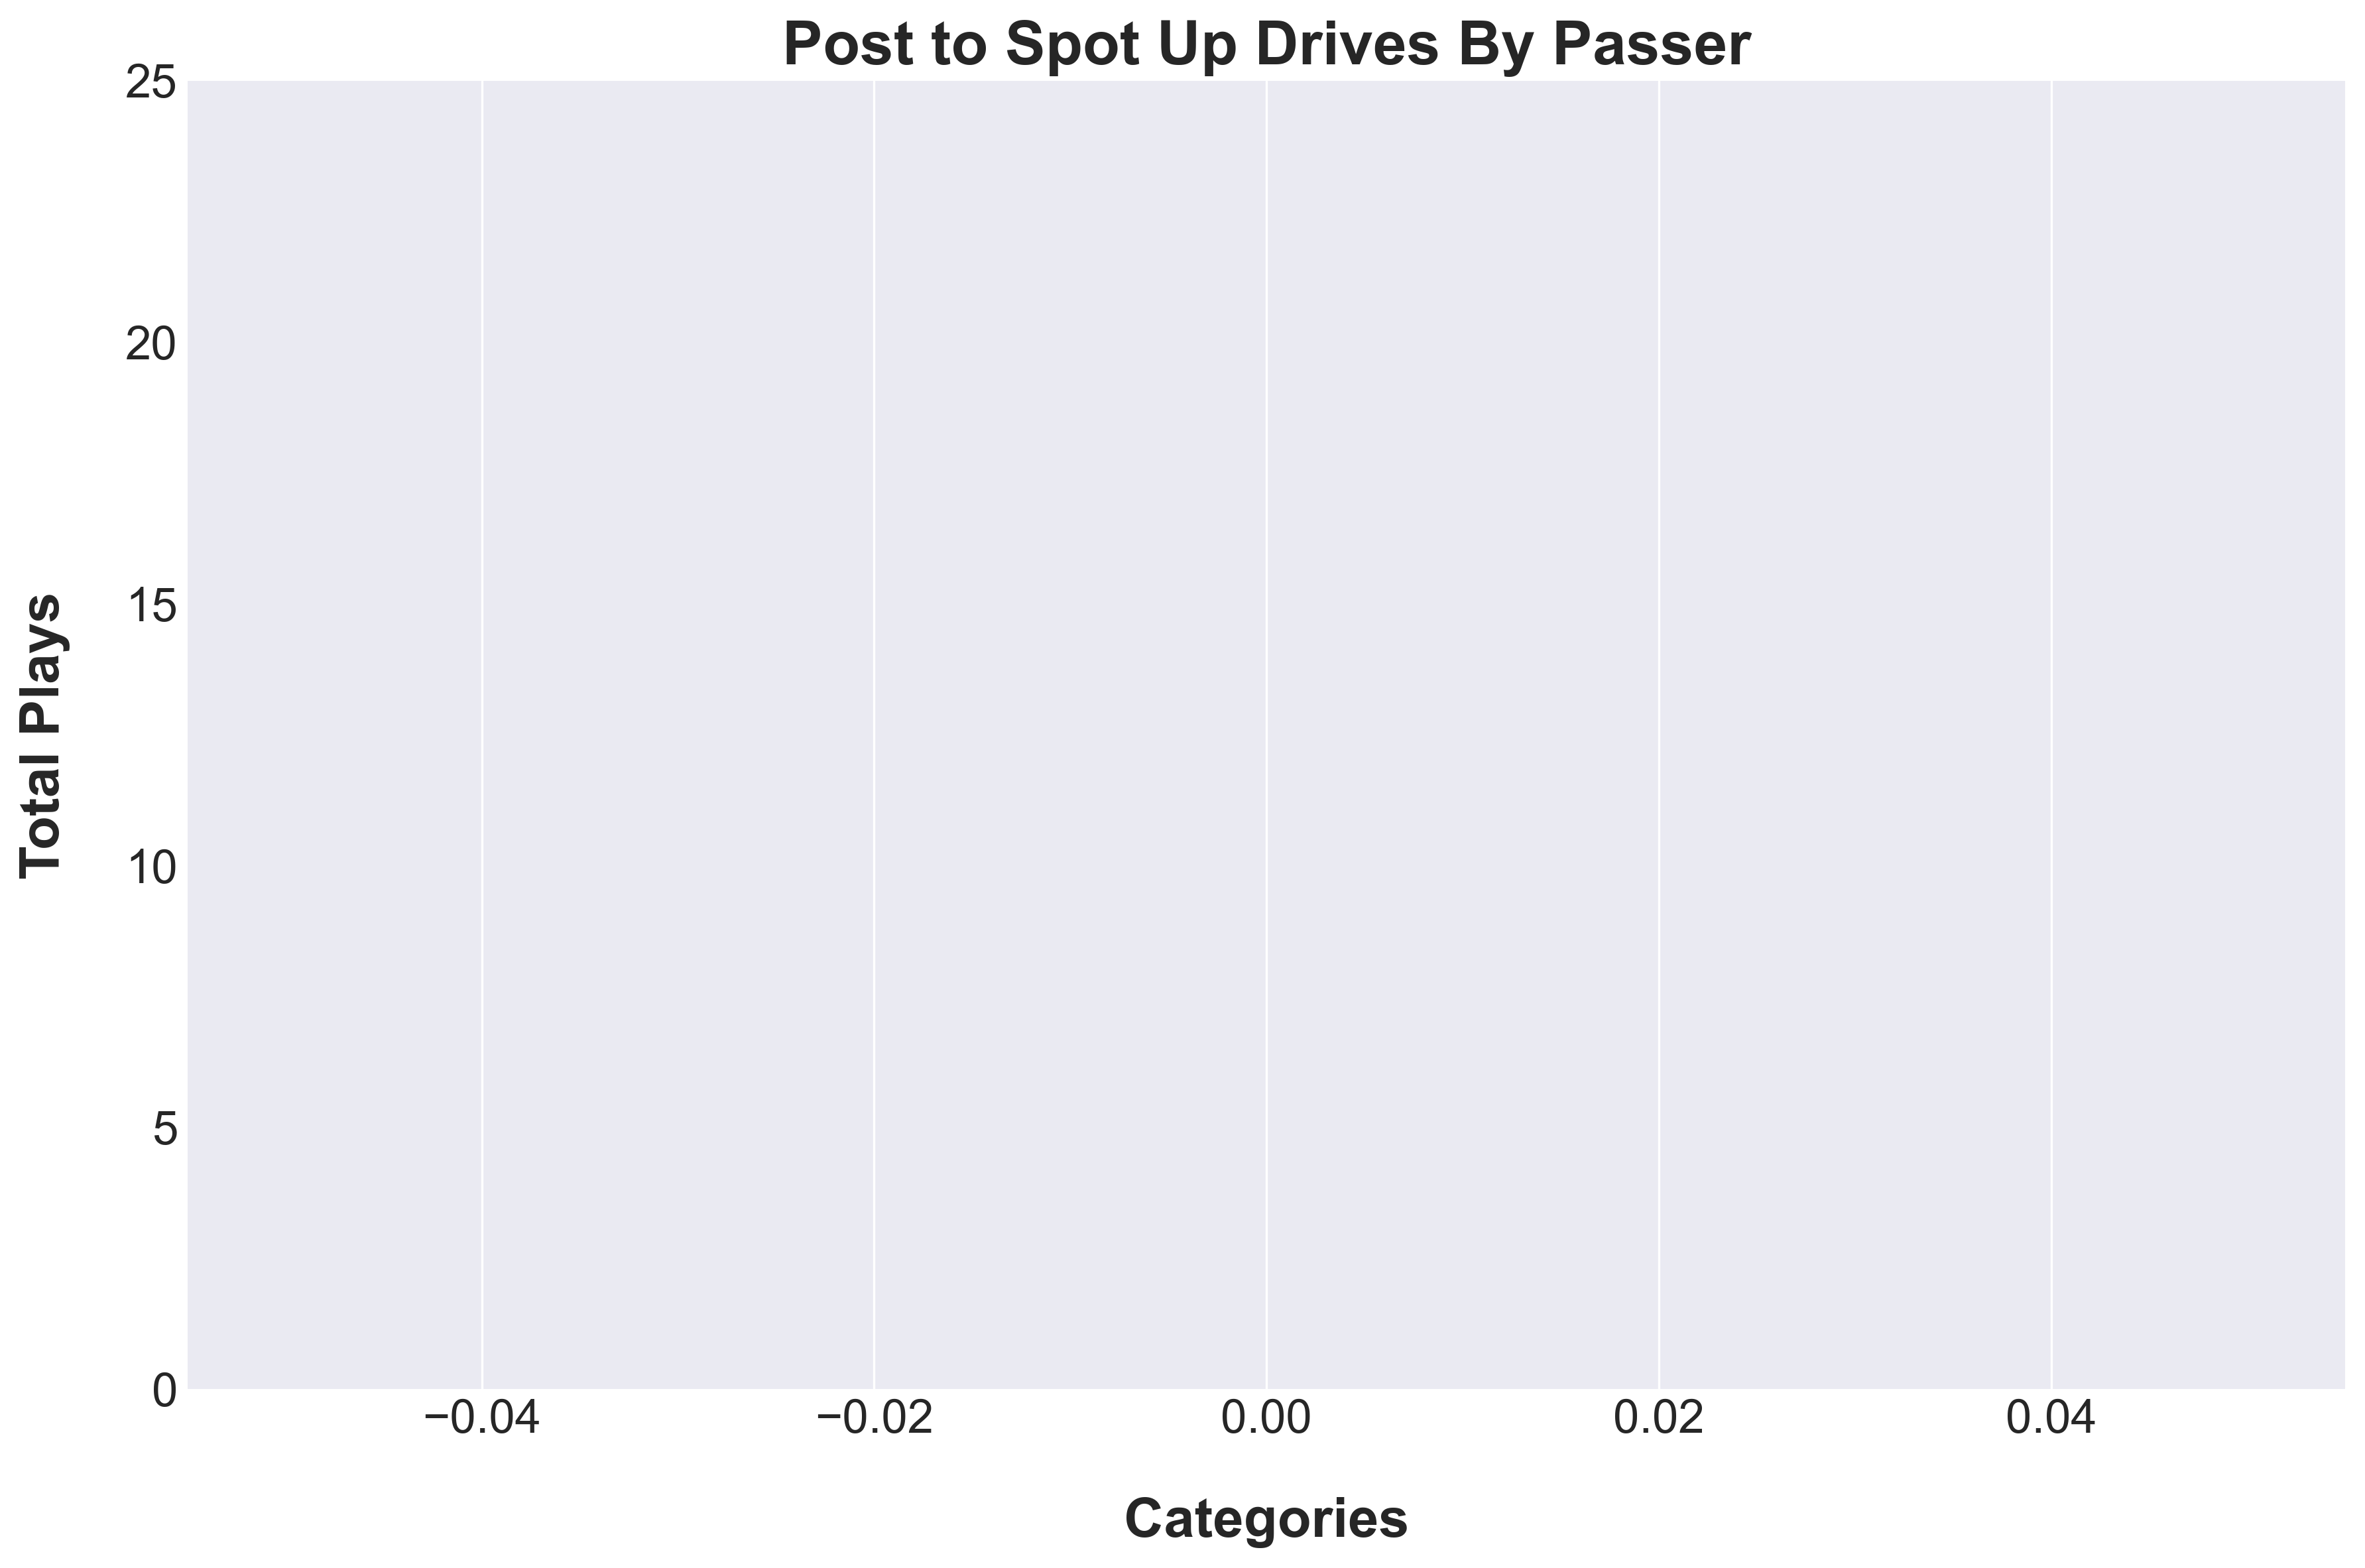
\includegraphics[width=\textwidth, height=.14\textheight]{images/SpotUp_PostDrivesPlayer_Freq.png} % Adjust the width of the image to fit
    \end{minipage}
\end{table}

\vspace{-1em} % Add vertical space before the line (optional)
\vspace{-1em} % Add vertical space after the line (optional)

% Iso -> Drive Stats by Passer
\begin{table}[H]
    \raisebox{3em}{ % Adjust this value to shift the tables vertically
    \begin{minipage}[t]{0.6\textwidth} % Left side (table) takes 85% of the width
        \flushleft
        \centering % Centering the title and the table
        \text{Iso - Drive Stats by Passer} % Title above the table in bold
        \vskip .25em % Adds vertical space between title and table
        \scalebox{.55}{ % Scale the entire table down by half
            \renewcommand{\arraystretch}{1.4} % Adjust the number to increase or decrease row spacing
            \begin{tabular}{
            >{\centering\arraybackslash}p{3cm} 
            >{\centering\arraybackslash}p{.75cm} 
            >{\centering\arraybackslash}p{.75cm} 
            >{\centering\arraybackslash}p{.75cm} 
            >{\centering\arraybackslash}p{.75cm}
            >{\centering\arraybackslash}p{.75cm} 
            >{\centering\arraybackslash}p{.75cm} 
            >{\centering\arraybackslash}p{.75cm} 
            >{\centering\arraybackslash}p{.75cm}
            >{\centering\arraybackslash}p{.75cm} 
            >{\centering\arraybackslash}p{.75cm}
            >{\centering\arraybackslash}p{.75cm} 
            >{\centering\arraybackslash}p{.75cm}}% Adjust column widths
            \toprule
            {\scriptsize \textbf{Player}} &
            {\scriptsize \textbf{Plays}} &
            {\scriptsize \textbf{3PA}} &
            {\scriptsize \textbf{3PM}} &
            {\scriptsize \textbf{3P\%}} & 
            {\scriptsize \textbf{2PA}} & 
            {\scriptsize \textbf{2PM}} & 
            {\scriptsize \textbf{2P\%}} & 
            {\scriptsize \textbf{MiA}} & 
            {\scriptsize \textbf{MiM}} &
            {\scriptsize \textbf{Mi\%}} &
            {\scriptsize \textbf{TO}} &
            {\scriptsize \textbf{Foul}} \\
            \midrule
            
                
            
                
            
                
            
                
            
                
                    
                
            
                
            
                
            
                
            
                
            
                
            
                
            
                
            
                
            
                
            
                
            
                
            
                
            
                
            
                
            
                
            
                
            
                
            

            \bottomrule
        \end{tabular}
        } % End of \scalebox
    \end{minipage}
    } % End of raisebox, closing the adjustment
    \hfill % This adds some flexible space between the table and the image
    \begin{minipage}[c]{0.35\textwidth} % Right side (image) takes 10% of the width
        \flushright
        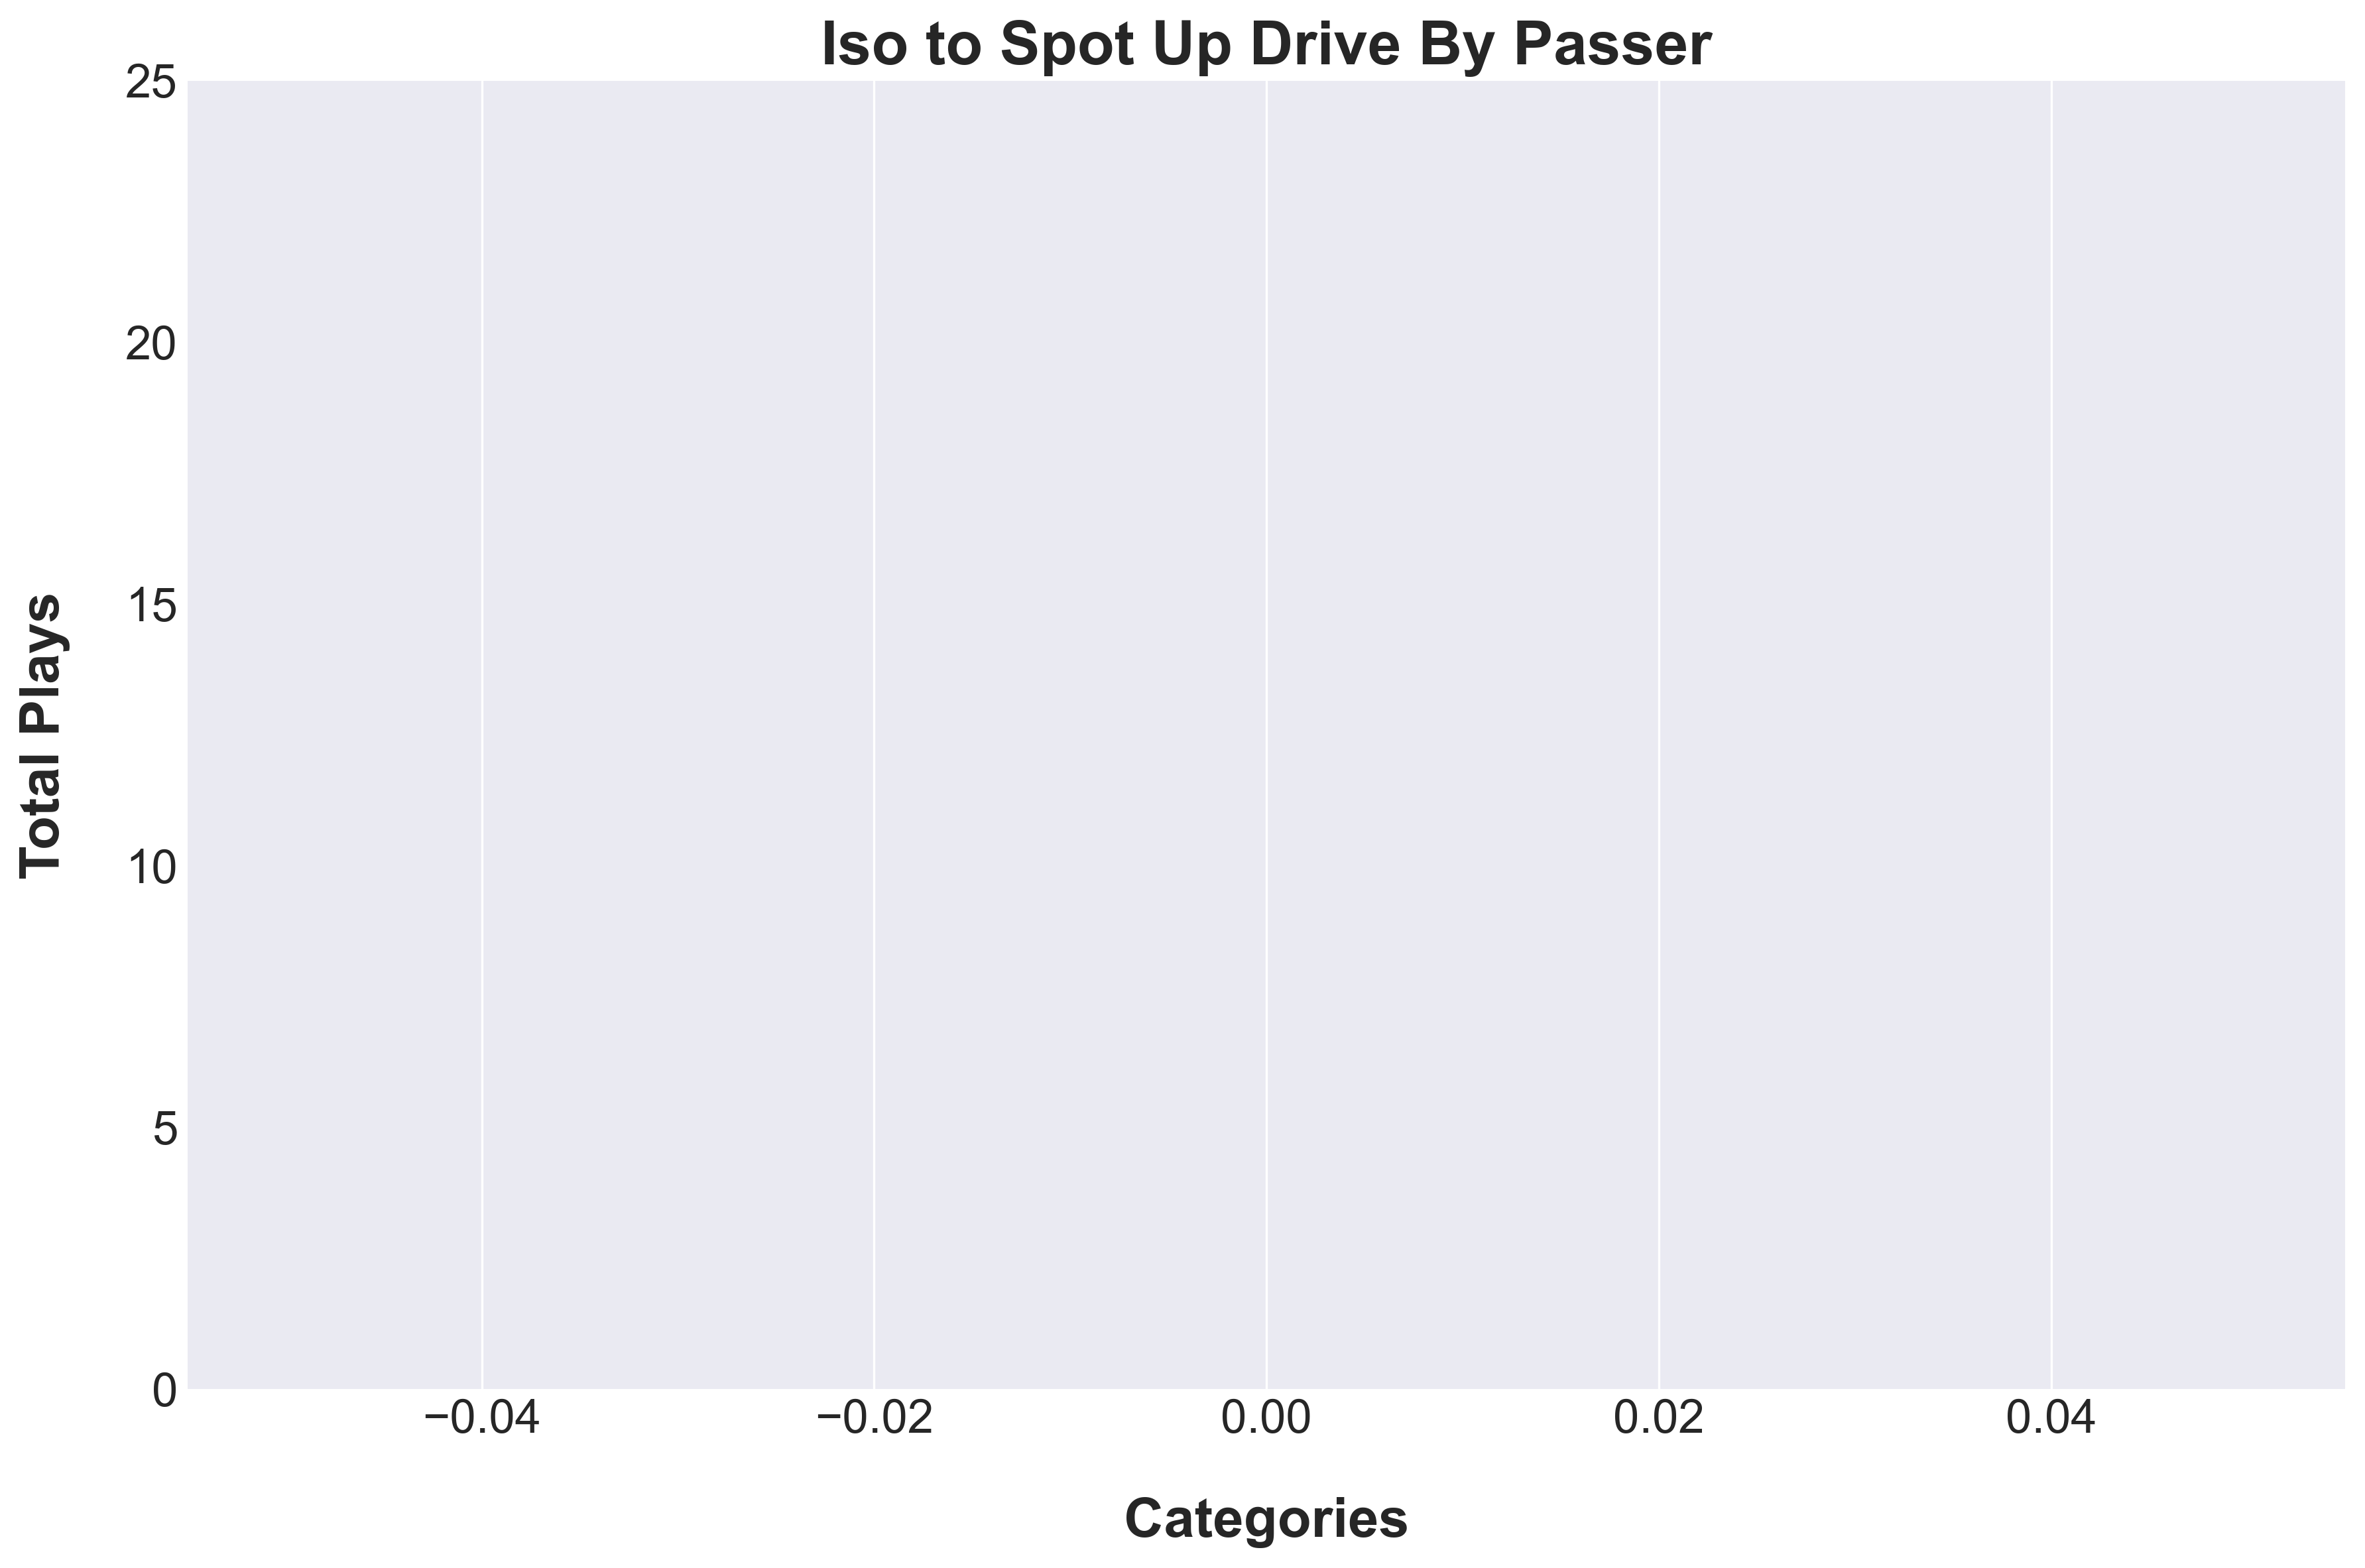
\includegraphics[width=\textwidth, height=.14\textheight]{images/SpotUp_IsoDrivesPlayer_Freq.png} % Adjust the width of the image to fit
    \end{minipage}
\end{table}

\vspace{-1em} % Add vertical space before the line (optional)
\vspace{-1em} % Add vertical space after the line (optional)

% PNR -> Drive Stats by Passer
\begin{table}[H]
    \raisebox{3em}{ % Adjust this value to shift the tables vertically
    \begin{minipage}[t]{0.6\textwidth} % Left side (table) takes 85% of the width
        \flushleft
        \centering % Centering the title and the table
        \text{PNR - Drive Stats by Passer} % Title above the table in bold
        \vskip .25em % Adds vertical space between title and table
        \scalebox{.55}{ % Scale the entire table down by half
            \renewcommand{\arraystretch}{1.4} % Adjust the number to increase or decrease row spacing
            \begin{tabular}{
            >{\centering\arraybackslash}p{3cm} 
            >{\centering\arraybackslash}p{.75cm} 
            >{\centering\arraybackslash}p{.75cm} 
            >{\centering\arraybackslash}p{.75cm} 
            >{\centering\arraybackslash}p{.75cm}
            >{\centering\arraybackslash}p{.75cm} 
            >{\centering\arraybackslash}p{.75cm} 
            >{\centering\arraybackslash}p{.75cm} 
            >{\centering\arraybackslash}p{.75cm}
            >{\centering\arraybackslash}p{.75cm} 
            >{\centering\arraybackslash}p{.75cm}
            >{\centering\arraybackslash}p{.75cm}
            >{\centering\arraybackslash}p{.75cm} 
            >{\centering\arraybackslash}p{.75cm}}% Adjust column widths
            \toprule
            {\scriptsize \textbf{Player}} &
            {\scriptsize \textbf{Plays}} &
            {\scriptsize \textbf{3PA}} &
            {\scriptsize \textbf{3PM}} &
            {\scriptsize \textbf{3P\%}} & 
            {\scriptsize \textbf{2PA}} & 
            {\scriptsize \textbf{2PM}} & 
            {\scriptsize \textbf{2P\%}} & 
            {\scriptsize \textbf{MiA}} & 
            {\scriptsize \textbf{MiM}} &
            {\scriptsize \textbf{Mi\%}} &
            {\scriptsize \textbf{TO}} &
            {\scriptsize \textbf{Foul}} \\
            \midrule
            
                
            
                
            
                
            
                
            
                
            
                
            
                
            
                
            
                
                    
                        Brock Bowen & 
                        2 & 
                        0 & 
                        0 & 
                        - & 
                        1 & 
                        1 & 
                        100.0 & 
                        0 & 
                        0 & 
                        - & 
                        1 & 
                        0 \\
                    
                        Brody Brown & 
                        1 & 
                        0 & 
                        0 & 
                        - & 
                        0 & 
                        0 & 
                        - & 
                        0 & 
                        0 & 
                        - & 
                        1 & 
                        0 \\
                    
                        Mark Osime & 
                        1 & 
                        0 & 
                        0 & 
                        - & 
                        1 & 
                        0 & 
                        0.0 & 
                        0 & 
                        0 & 
                        - & 
                        0 & 
                        0 \\
                    
                
            
                
            
                
            
                
            
                
            
                
            
                
            
                
            
                
            
                
            
                
            
                
            
                
            
                
            

            \bottomrule
        \end{tabular}
        } % End of \scalebox
    \end{minipage}
    } % End of raisebox, closing the adjustment
    \hfill % This adds some flexible space between the table and the image
    \begin{minipage}[c]{0.35\textwidth} % Right side (image) takes 10% of the width
        \flushright
        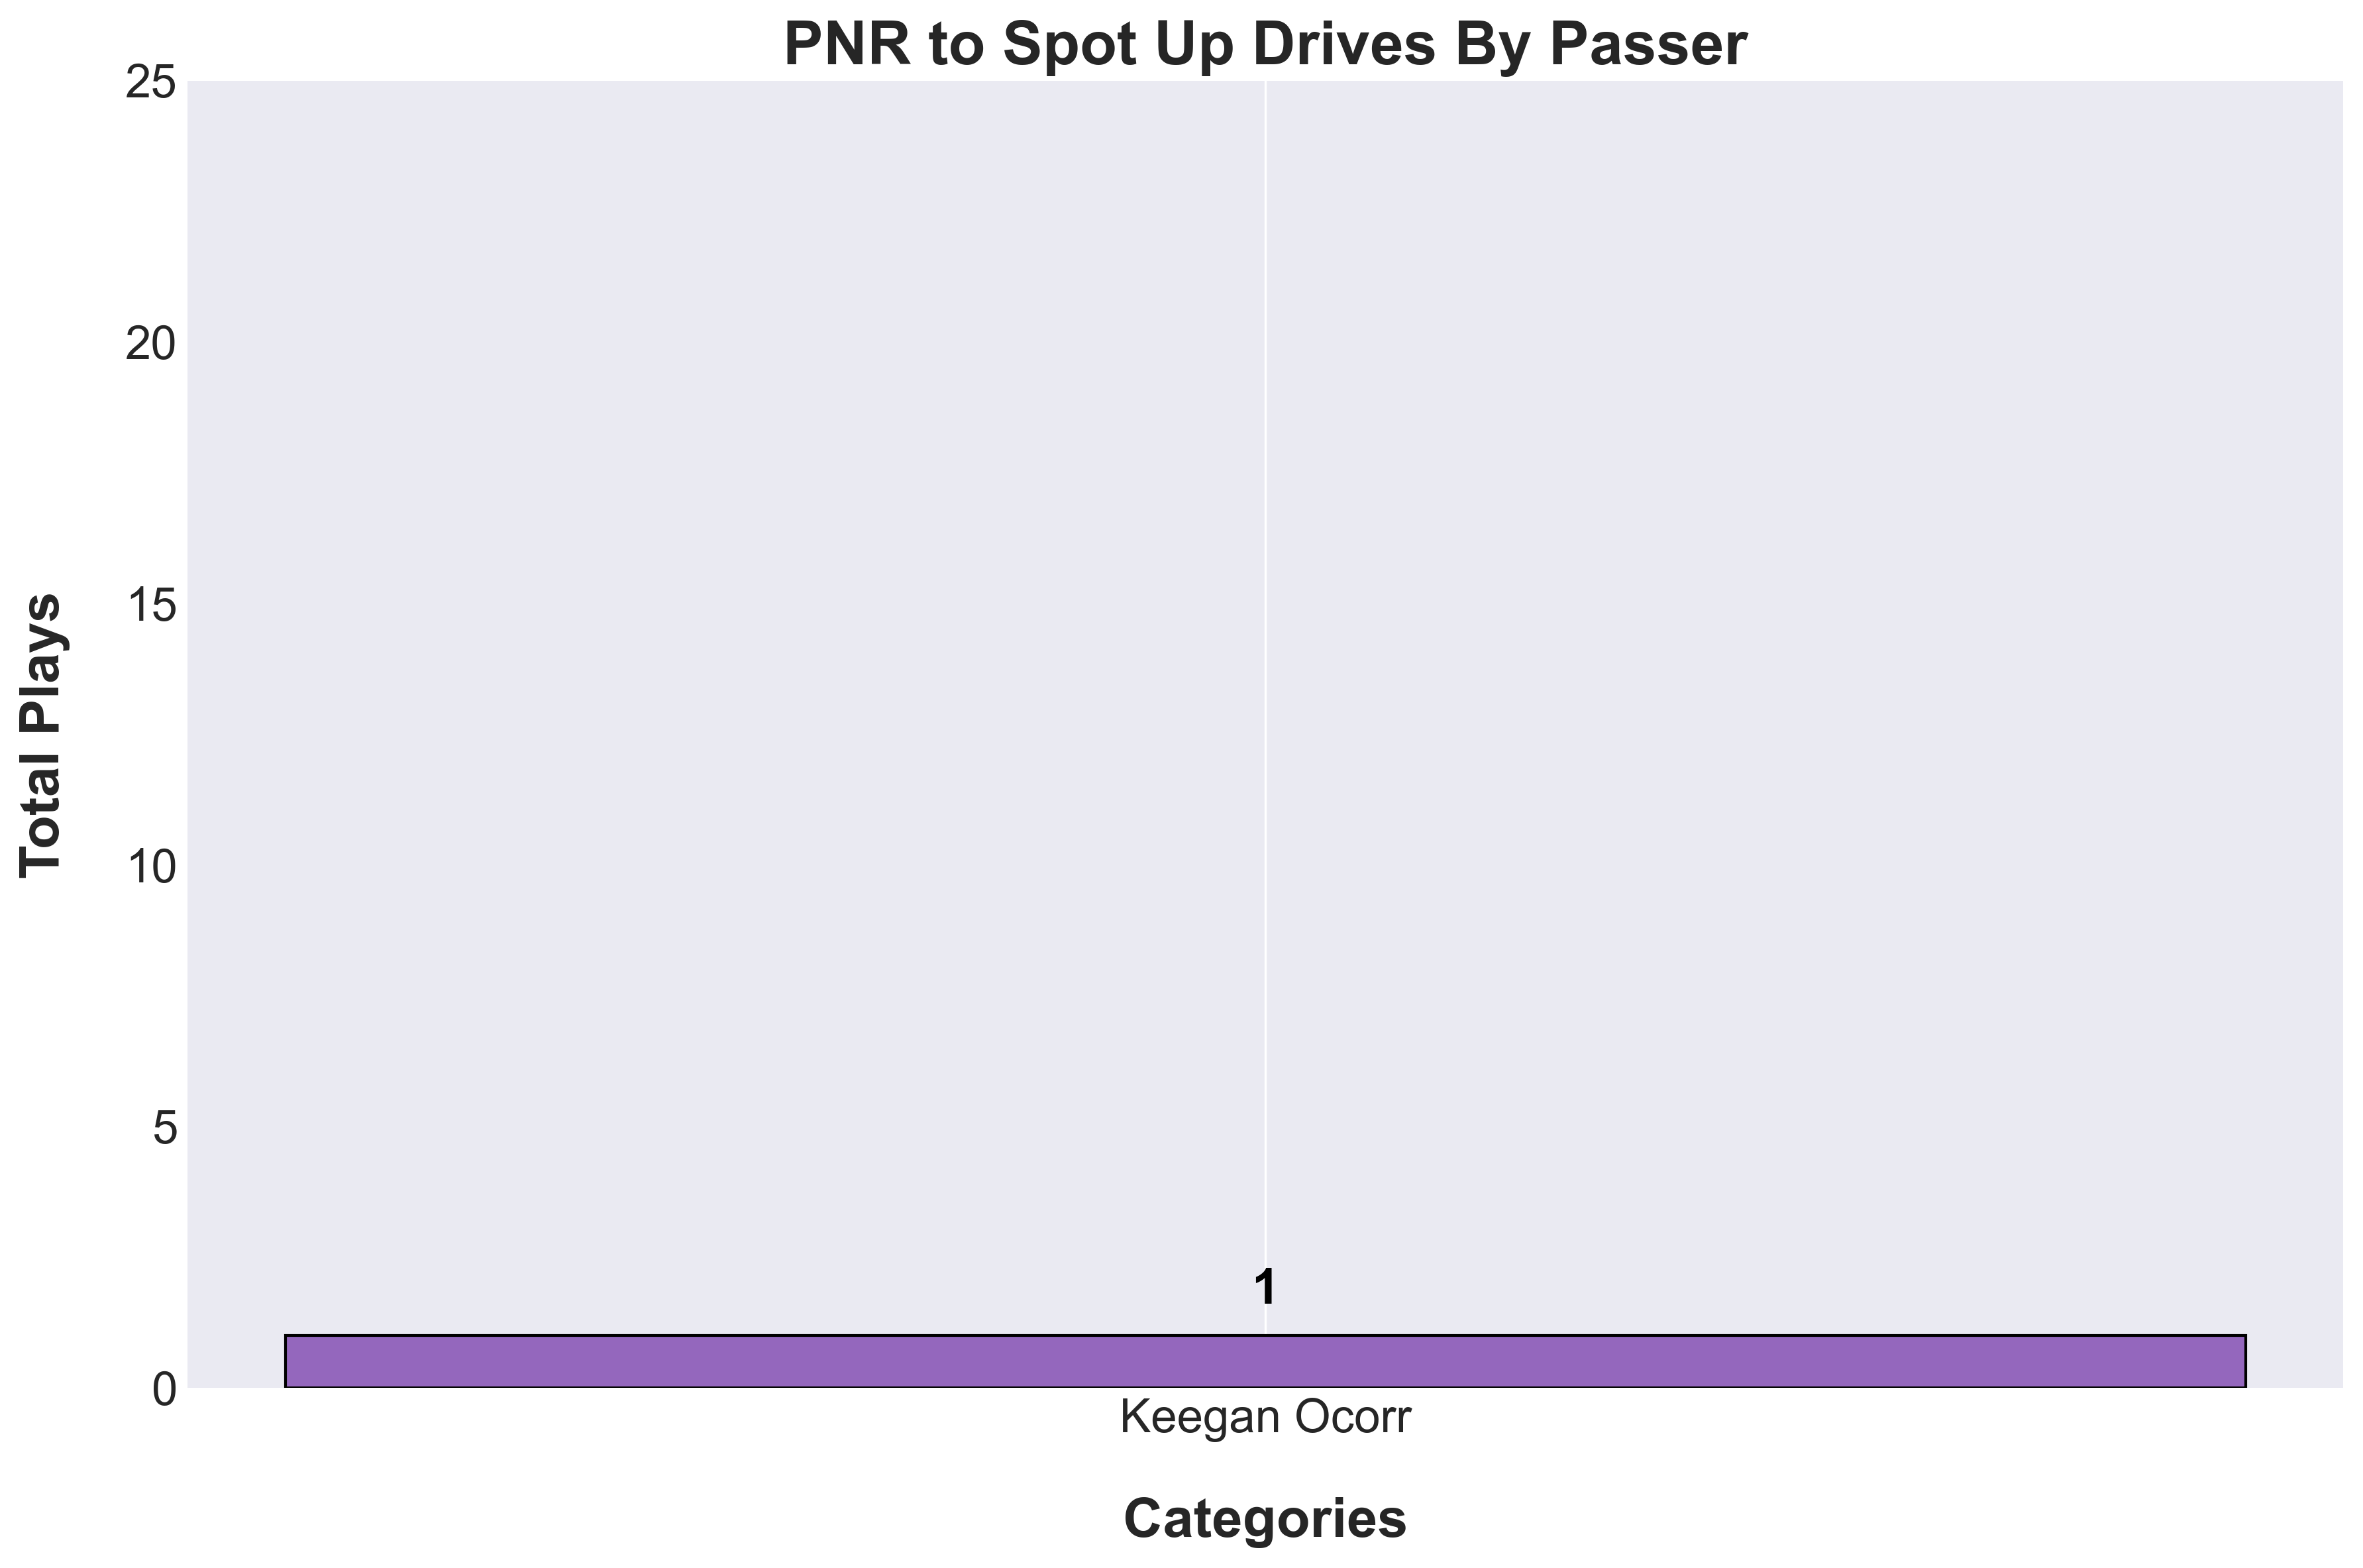
\includegraphics[width=\textwidth, height=.14\textheight]{images/SpotUp_PnrDrivesPlayer_Freq.png} % Adjust the width of the image to fit
    \end{minipage}
\end{table}

\vspace{-1em} % Add vertical space before the line (optional)
\hrule height 1pt width 1\textwidth % Adjust height and width
\vspace{1em} % Add vertical space after the line (optional)
\clearpage











% ----------------------
% Off Screen Visuals and Insights Section
% ----------------------
\subsection{Off Screens}
\vspace{1.25em} % Add vertical space before the line (optional)
\textbf{Key Notes on Off Screen Tendencies}
\vspace{0.5em} % Add space between the title and the itemized list

\begin{itemize}
    \item Off Screens make up x\% of players offensive load
    \vspace{0.3em} % Add space between the title and the itemized list
    \item Player is more efficient when coming off his left shoulder and get shots off of his left shoulder x\% of the time.
\end{itemize}

\vspace{1em} % Add vertical space before the line (optional)
\hrule height 1pt width 1\textwidth % Adjust height and width
\vspace{0em} % Add vertical space after the line (optional)

\subsubsection{Off Screen Shot Statistics}

% All Off Screen Statistics Table w/ room for insights
\begin{table}[H]
    \centering
    \begin{minipage}[t]{0.6\textwidth} % Left side (table) takes 85% of the width
        %\flushright
        \centering % Centering the title and the table
        \text{Total Off Screen Shot Statistics} % Title above the table in bold
        \vskip .25em % Adds vertical space between title and table
        \scalebox{.85}{ % Scale the entire table down by half
            \scriptsize % Reduce the font size
            \begin{tabular}{
            >{\centering\arraybackslash}p{.75cm} 
            >{\centering\arraybackslash}p{.5cm} 
            >{\centering\arraybackslash}p{.5cm} 
            >{\centering\arraybackslash}p{.5cm}
            >{\centering\arraybackslash}p{.5cm} 
            >{\centering\arraybackslash}p{.5cm} 
            >{\centering\arraybackslash}p{.5cm} 
            >{\centering\arraybackslash}p{.5cm}
            >{\centering\arraybackslash}p{.5cm} 
            >{\centering\arraybackslash}p{.5cm}
            >{\centering\arraybackslash}p{.75cm}
            >{\centering\arraybackslash}p{.5cm} 
            >{\centering\arraybackslash}p{.5cm}}% Adjust column widths
            \toprule
            \textbf{Plays} &
            \textbf{3PA} &
            \textbf{3PM} &
            \textbf{3P\%} & 
            \textbf{2PA} & 
            \textbf{2PM} & 
            \textbf{2P\%} & 
            \textbf{MiA} & 
            \textbf{MiM} &
            \textbf{Mi\%} &
            \textbf{EFG\%} &
            \textbf{TO} &
            \textbf{Foul} \\
            \midrule
            
                
                    13 & 3 & 0 &
                    0.0 & 
                    9 & 4 &
                    44.44 &
                    2 & 0 &
                    0.0 &
                    33.33 &
                    1 & 0 \\
                
            
                
            
                
            
                
            
                
            
                
            
                
            
                
            
                
            
                
            
                
            
                
            
                
            


            \bottomrule
            \end{tabular}
        }
    \end{minipage}
\end{table}

\vspace{0em} % Add vertical space before the line (optional)
%\hrule height 1pt width 1\textwidth % Adjust height and width
\vspace{-1em} % Add vertical space after the line (optional)

% Off Screen Stats for shooting off Left vs Right Shoulder
\begin{table}[H]
    \raisebox{3em}{ % Adjust this value to shift the tables vertically
    \begin{minipage}[t]{0.6\textwidth} % Left side (table) takes 85% of the width
        \flushleft
        \centering % Centering the title and the table
        \text{Shots Running Off Specific Shoulder Statistics} % Title above the table in bold
        \vskip .25em % Adds vertical space between title and table
        \scalebox{.6}{ % Scale the entire table down by half
            \renewcommand{\arraystretch}{1.4} % Adjust the number to increase or decrease row spacing
            \begin{tabular}{
            >{\centering\arraybackslash}p{1.75cm} 
            >{\centering\arraybackslash}p{.75cm} 
            >{\centering\arraybackslash}p{.75cm} 
            >{\centering\arraybackslash}p{.75cm} 
            >{\centering\arraybackslash}p{.75cm}
            >{\centering\arraybackslash}p{.75cm} 
            >{\centering\arraybackslash}p{.75cm} 
            >{\centering\arraybackslash}p{.75cm} 
            >{\centering\arraybackslash}p{.75cm}
            >{\centering\arraybackslash}p{.75cm} 
            >{\centering\arraybackslash}p{.75cm}
            >{\centering\arraybackslash}p{.75cm} 
            >{\centering\arraybackslash}p{.75cm}}% Adjust column widths
            \toprule
            {\scriptsize \textbf{PlayType}} &
            {\scriptsize \textbf{Plays}} &
            {\scriptsize \textbf{3PA}} &
            {\scriptsize \textbf{3PM}} &
            {\scriptsize \textbf{3P\%}} & 
            {\scriptsize \textbf{2PA}} & 
            {\scriptsize \textbf{2PM}} & 
            {\scriptsize \textbf{2P\%}} & 
            {\scriptsize \textbf{MiA}} & 
            {\scriptsize \textbf{MiM}} &
            {\scriptsize \textbf{Mi\%}} &
            {\scriptsize \textbf{TO}} &
            {\scriptsize \textbf{Foul}} \\
            \midrule
            
                
            
                
            
                
                    Left & 3 & 0 & 0 &
                    - & 
                    3 & 1 &
                    33.33 &
                    1 & 0 &
                    0.0 &
                    0 & 0 \\
                
            
                
                    Right & 10 & 3 & 0 &
                    0.0 & 
                    6 & 3 &
                    50.0 &
                    1 & 0 &
                    0.0 &
                    1 & 0 \\
                
            
                
            
                
            
                
            
                
            
                
            
                
            
                
            
                
            
                
            

            \bottomrule
        \end{tabular}
        } % End of \scalebox
    \end{minipage}
    } % End of raisebox, closing the adjustment
    \hfill % This adds some flexible space between the table and the image
    \begin{minipage}[c]{0.35\textwidth} % Right side (image) takes 10% of the width
        \flushright
        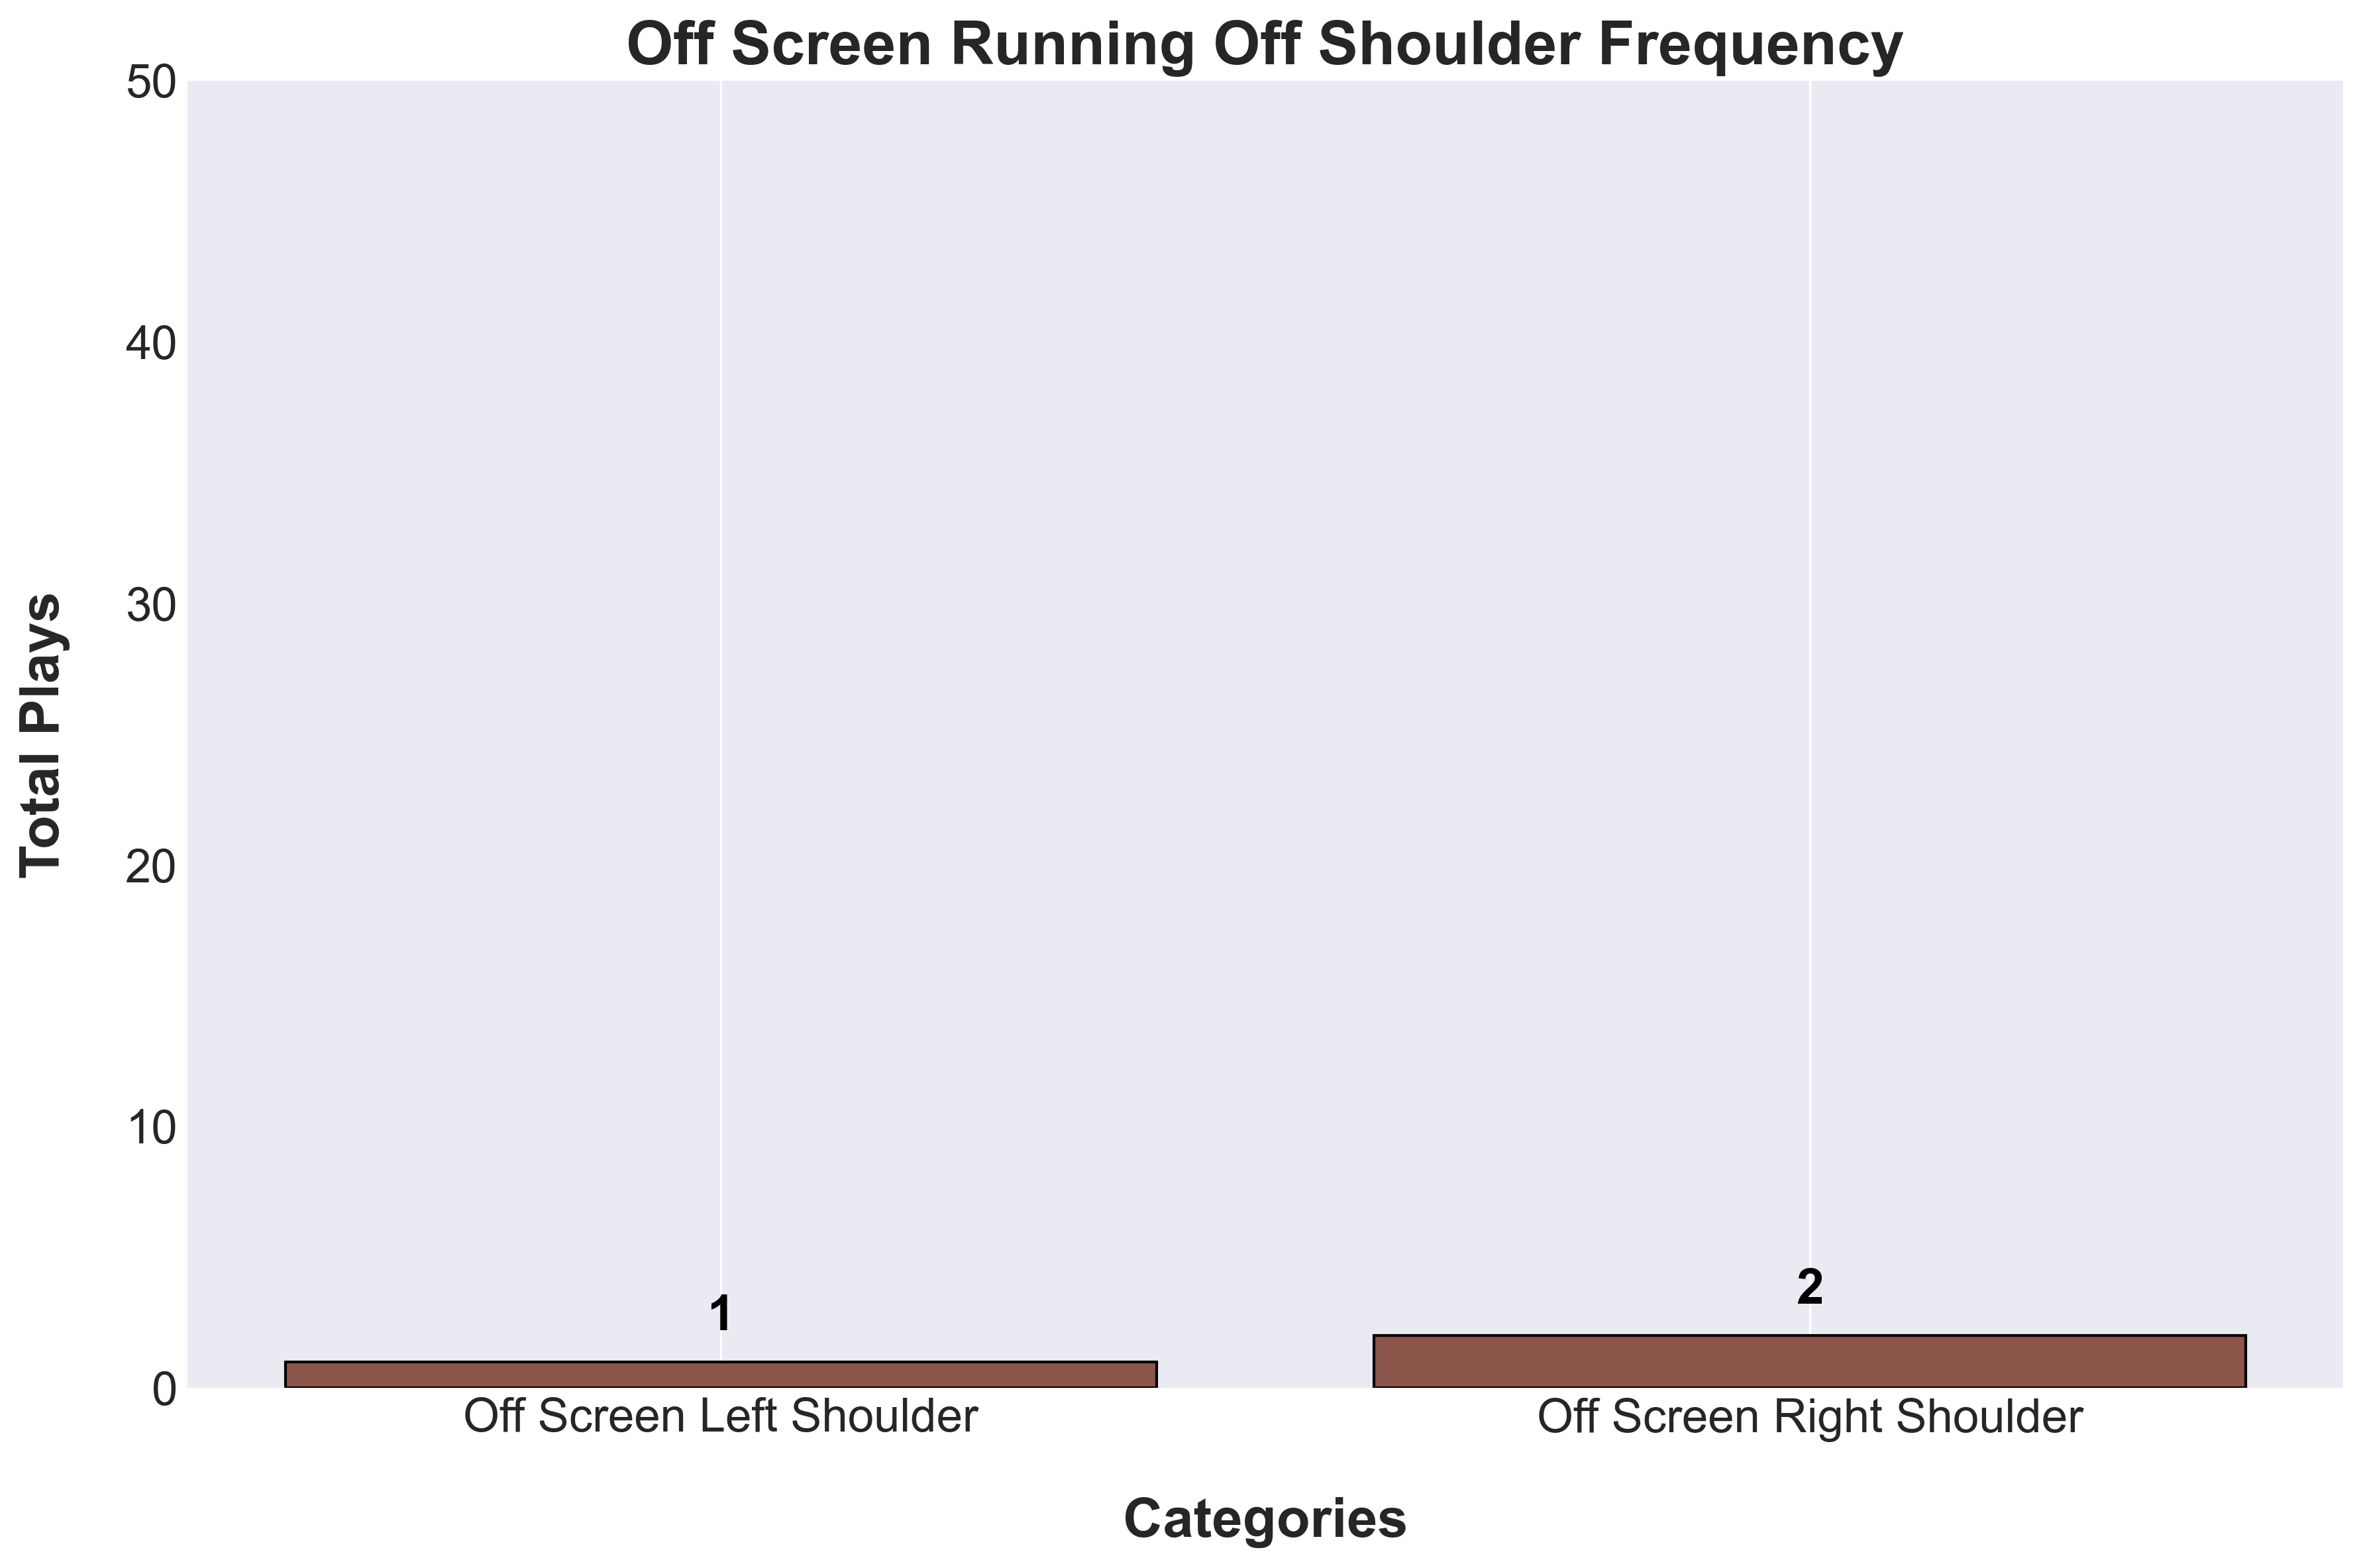
\includegraphics[width=\textwidth, height=.14\textheight]{images/OffScreen_Shoulder_Freq.png} % Adjust the width of the image to fit
    \end{minipage}
\end{table}

\vspace{-1em} % Add vertical space before the line (optional)
%\hrule height 1pt width 1\textwidth % Adjust height and width
\vspace{-1em} % Add vertical space after the line (optional)

% Off Screen Type Statistics
\begin{table}[H]
    \raisebox{3.5em}{ % Adjust this value to shift the tables vertically
    \begin{minipage}[t]{0.6\textwidth} % Left side (table) takes 85% of the width
        \flushleft
        \centering % Centering the title and the table
        \text{Off Screen Type Statistics} % Title above the table in bold
        \vskip .25em % Adds vertical space between title and table
        \scalebox{.6}{ % Scale the entire table down by half
            \renewcommand{\arraystretch}{1.4} % Adjust the number to increase or decrease row spacing
            \begin{tabular}{
            >{\centering\arraybackslash}p{1.75cm} 
            >{\centering\arraybackslash}p{.75cm} 
            >{\centering\arraybackslash}p{.75cm} 
            >{\centering\arraybackslash}p{.75cm} 
            >{\centering\arraybackslash}p{.75cm}
            >{\centering\arraybackslash}p{.75cm} 
            >{\centering\arraybackslash}p{.75cm} 
            >{\centering\arraybackslash}p{.75cm} 
            >{\centering\arraybackslash}p{.75cm}
            >{\centering\arraybackslash}p{.75cm} 
            >{\centering\arraybackslash}p{.75cm}
            >{\centering\arraybackslash}p{.75cm} 
            >{\centering\arraybackslash}p{.75cm}}% Adjust column widths
            \toprule
            {\scriptsize \textbf{PlayType}} &
            {\scriptsize \textbf{Plays}} &
            {\scriptsize \textbf{3PA}} &
            {\scriptsize \textbf{3PM}} &
            {\scriptsize \textbf{3P\%}} & 
            {\scriptsize \textbf{2PA}} & 
            {\scriptsize \textbf{2PM}} & 
            {\scriptsize \textbf{2P\%}} & 
            {\scriptsize \textbf{MiA}} & 
            {\scriptsize \textbf{MiM}} &
            {\scriptsize \textbf{Mi\%}} &
            {\scriptsize \textbf{TO}} &
            {\scriptsize \textbf{Foul}} \\
            \midrule
            
                
            
                
            
                
            
                
            
                
                    Flare & 3 & 0 & 0 &
                    - & 
                    3 & 1 &
                    33.33 &
                    1 & 0 &
                    0.0 &
                    0 & 0 \\
                
            
                
                    Straight & 9 & 3 & 0 &
                    0.0 & 
                    5 & 3 &
                    60.0 &
                    1 & 0 &
                    0.0 &
                    1 & 0 \\
                
            
                
                    Curl & 1 & 0 & 0 &
                    - & 
                    1 & 0 &
                    0.0 &
                    0 & 0 &
                    - &
                    0 & 0 \\
                
            
                
            
                
            
                
            
                
            
                
            
                
            
            \bottomrule
        \end{tabular}
        } % End of \scalebox
    \end{minipage}
    } % End of raisebox, closing the adjustment
    \hfill
    \begin{minipage}[c]{0.35\textwidth} % Right side (image) takes 10% of the width
        \flushright
        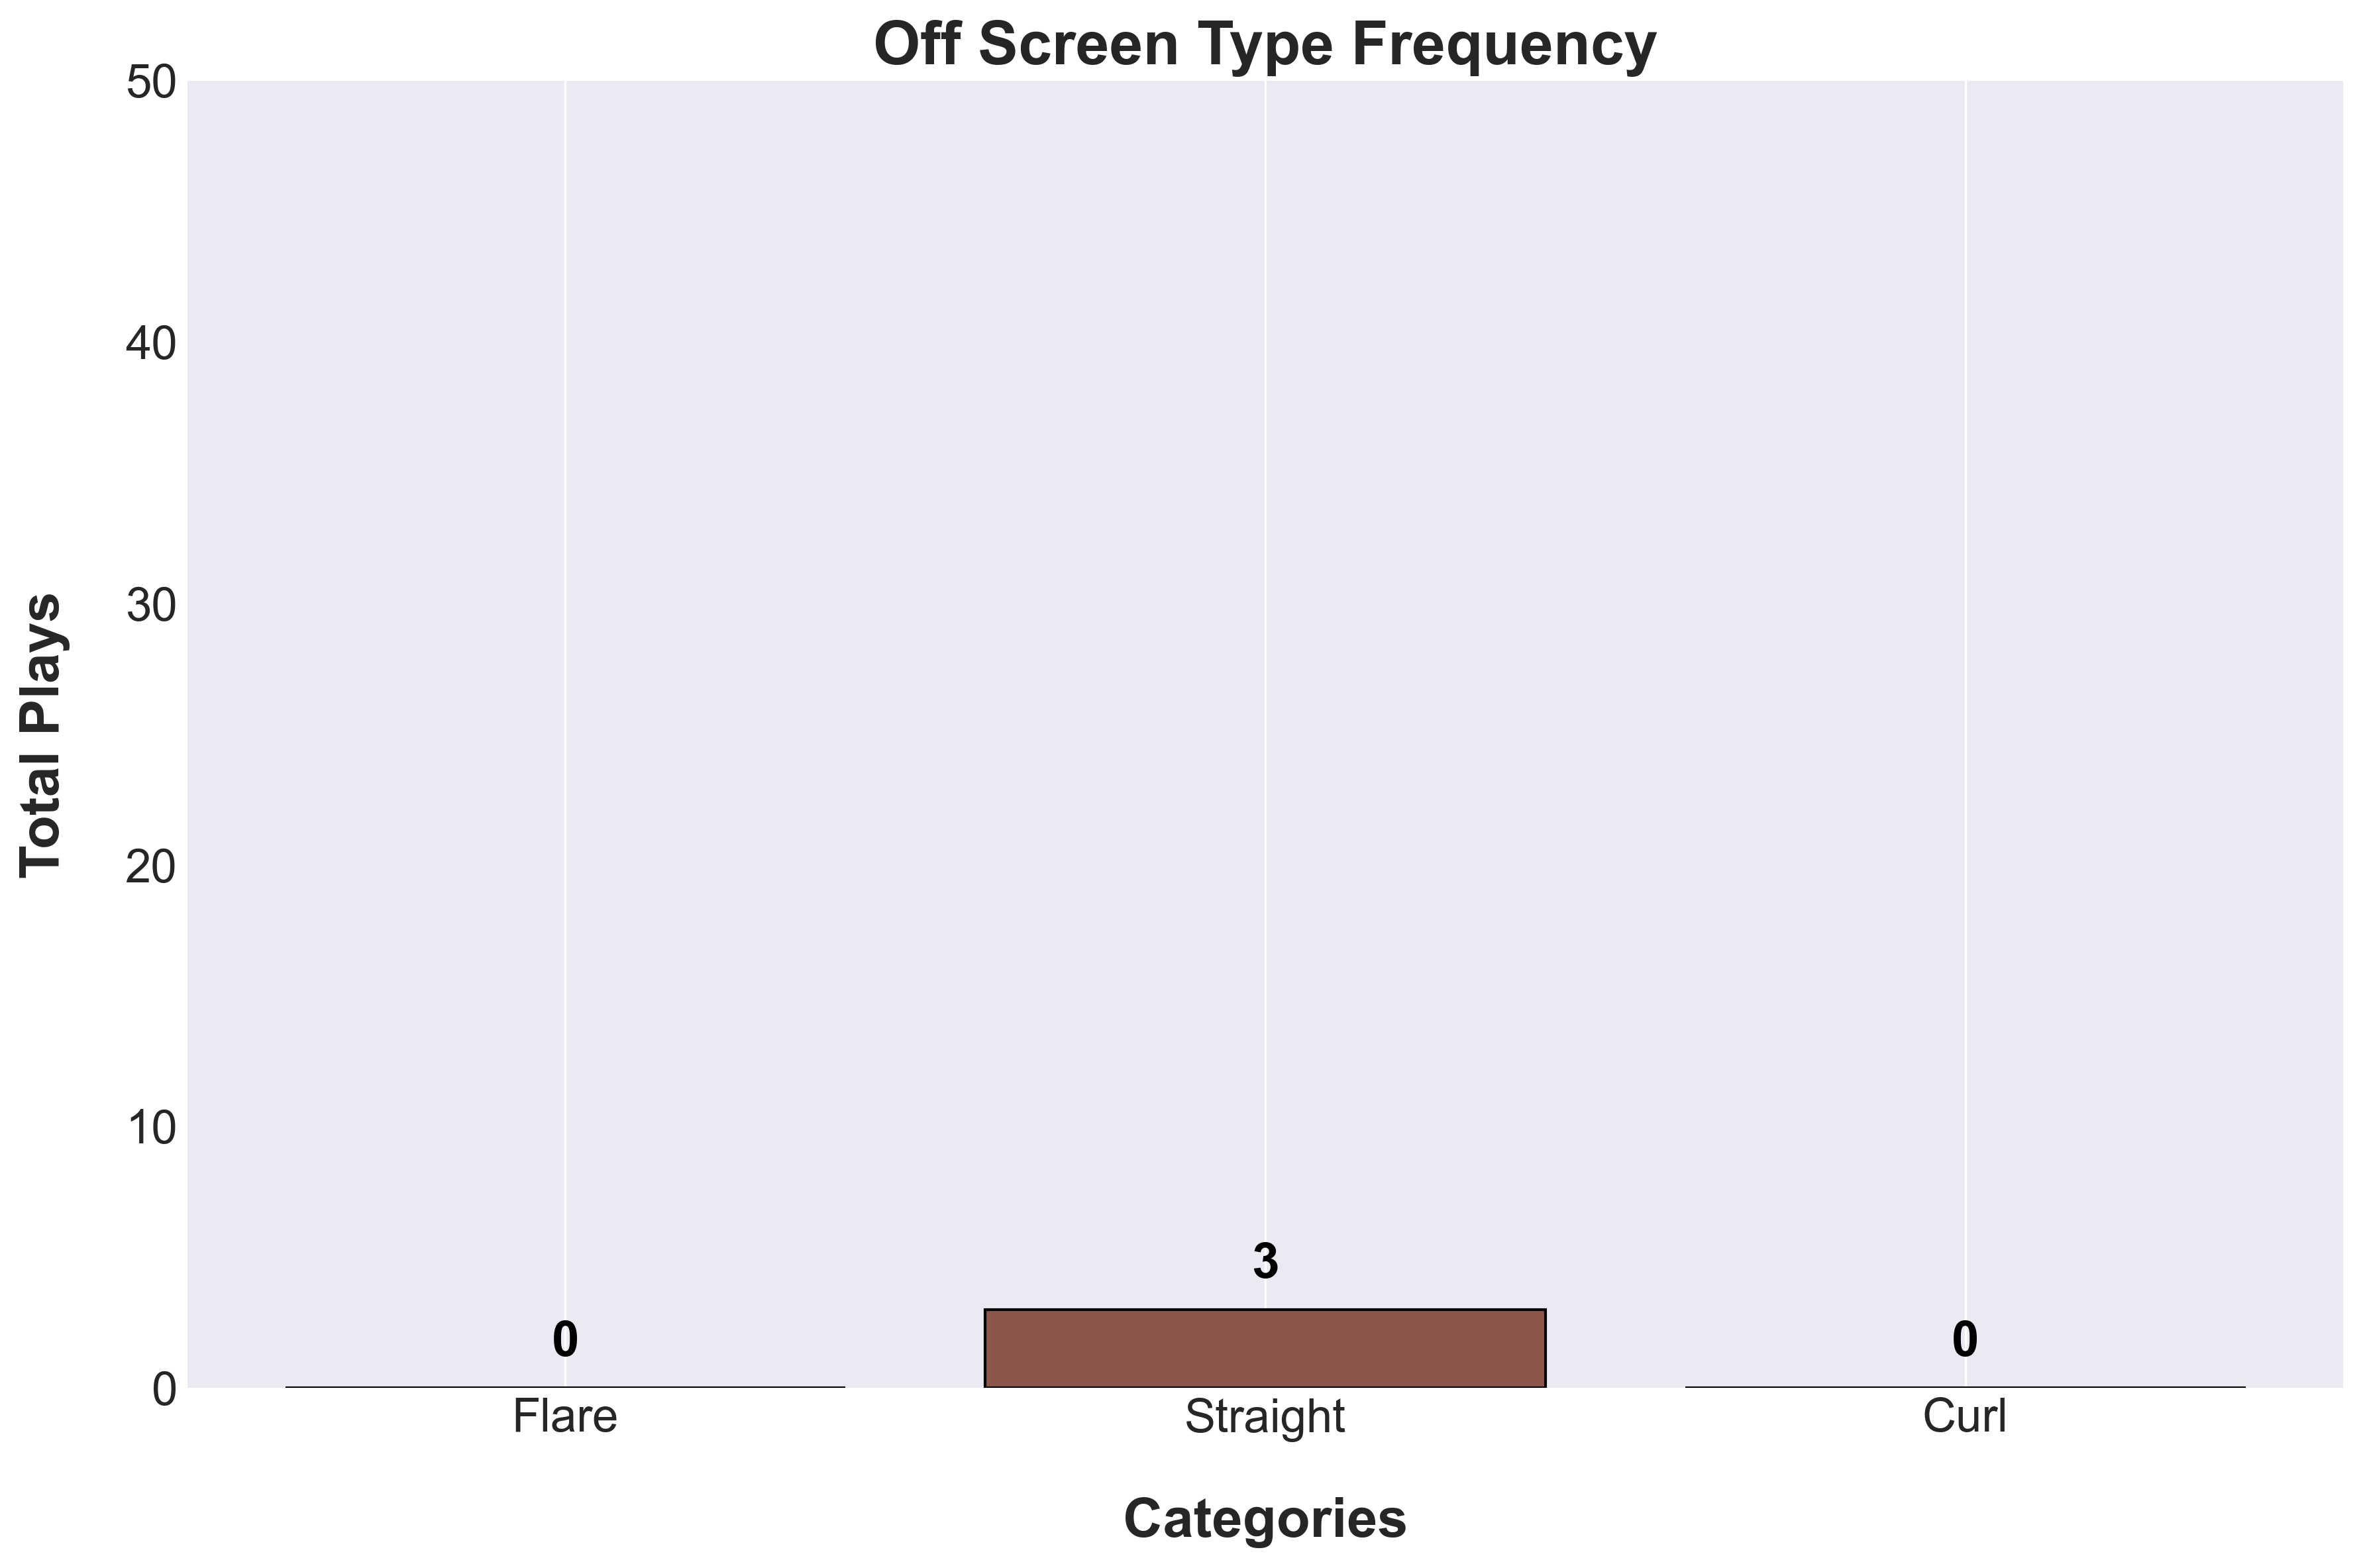
\includegraphics[width=\textwidth, height=.14\textheight]{images/OffScreen_Type_Freq.png} % Adjust the width of the image to fit
    \end{minipage}
    
\end{table}

\vspace{-1em} % Add vertical space before the line (optional)
%\hrule height 1pt width 1\textwidth % Adjust height and width
\vspace{-1em} % Add vertical space after the line (optional)

% Off Screen Stats for Combination of Shoulder and Type Stats
\begin{table}[H]
    \raisebox{4.5em}{ % Adjust this value to shift the tables vertically
    \begin{minipage}[t]{0.6\textwidth} % Left side (table) takes 85% of the width
        \flushleft
        \centering % Centering the title and the table
        \text{Off Screen Combination Statistics} % Title above the table in bold
        \vskip .25em % Adds vertical space between title and table
        \scalebox{.55}{ % Scale the entire table down by half
            \renewcommand{\arraystretch}{1.4} % Adjust the number to increase or decrease row spacing
            \begin{tabular}{
            >{\centering\arraybackslash}p{4cm} 
            >{\centering\arraybackslash}p{.75cm} 
            >{\centering\arraybackslash}p{.75cm} 
            >{\centering\arraybackslash}p{.75cm} 
            >{\centering\arraybackslash}p{.75cm}
            >{\centering\arraybackslash}p{.75cm} 
            >{\centering\arraybackslash}p{.75cm} 
            >{\centering\arraybackslash}p{.75cm} 
            >{\centering\arraybackslash}p{.75cm}
            >{\centering\arraybackslash}p{.75cm} 
            >{\centering\arraybackslash}p{.75cm}
            >{\centering\arraybackslash}p{.75cm} 
            >{\centering\arraybackslash}p{.75cm}}% Adjust column widths
            \toprule
            {\scriptsize \textbf{PlayType}} &
            {\scriptsize \textbf{Plays}} &
            {\scriptsize \textbf{3PA}} &
            {\scriptsize \textbf{3PM}} &
            {\scriptsize \textbf{3P\%}} & 
            {\scriptsize \textbf{2PA}} & 
            {\scriptsize \textbf{2PM}} & 
            {\scriptsize \textbf{2P\%}} & 
            {\scriptsize \textbf{MiA}} & 
            {\scriptsize \textbf{MiM}} &
            {\scriptsize \textbf{Mi\%}} &
            {\scriptsize \textbf{TO}} &
            {\scriptsize \textbf{Foul}} \\
            \midrule
            
                
            
                
            
                
            
                
            
                
            
                
            
                
            
                
            
                
                    Left - Straight & 1 & 0 & 0 &
                    - & 
                    1 & 1 &
                    100.0 &
                    0 & 0 &
                    - &
                    0 & 0 \\
                
            
                
                    Left - Curl & 1 & 0 & 0 &
                    - & 
                    1 & 0 &
                    0.0 &
                    0 & 0 &
                    - &
                    0 & 0 \\
                
            
                
                    Right - Flare & 2 & 0 & 0 &
                    - & 
                    2 & 1 &
                    50.0 &
                    0 & 0 &
                    - &
                    0 & 0 \\
                
            
                
                    Right - Straight & 8 & 3 & 0 &
                    0.0 & 
                    4 & 2 &
                    50.0 &
                    1 & 0 &
                    0.0 &
                    1 & 0 \\
                
            
                
            



            \bottomrule
        \end{tabular}
        } % End of \scalebox
    \end{minipage}
    } % End of raisebox, closing the adjustment
    \hfill % This adds some flexible space between the table and the image
    \begin{minipage}[c]{0.35\textwidth} % Right side (image) takes 10% of the width
        \flushright
        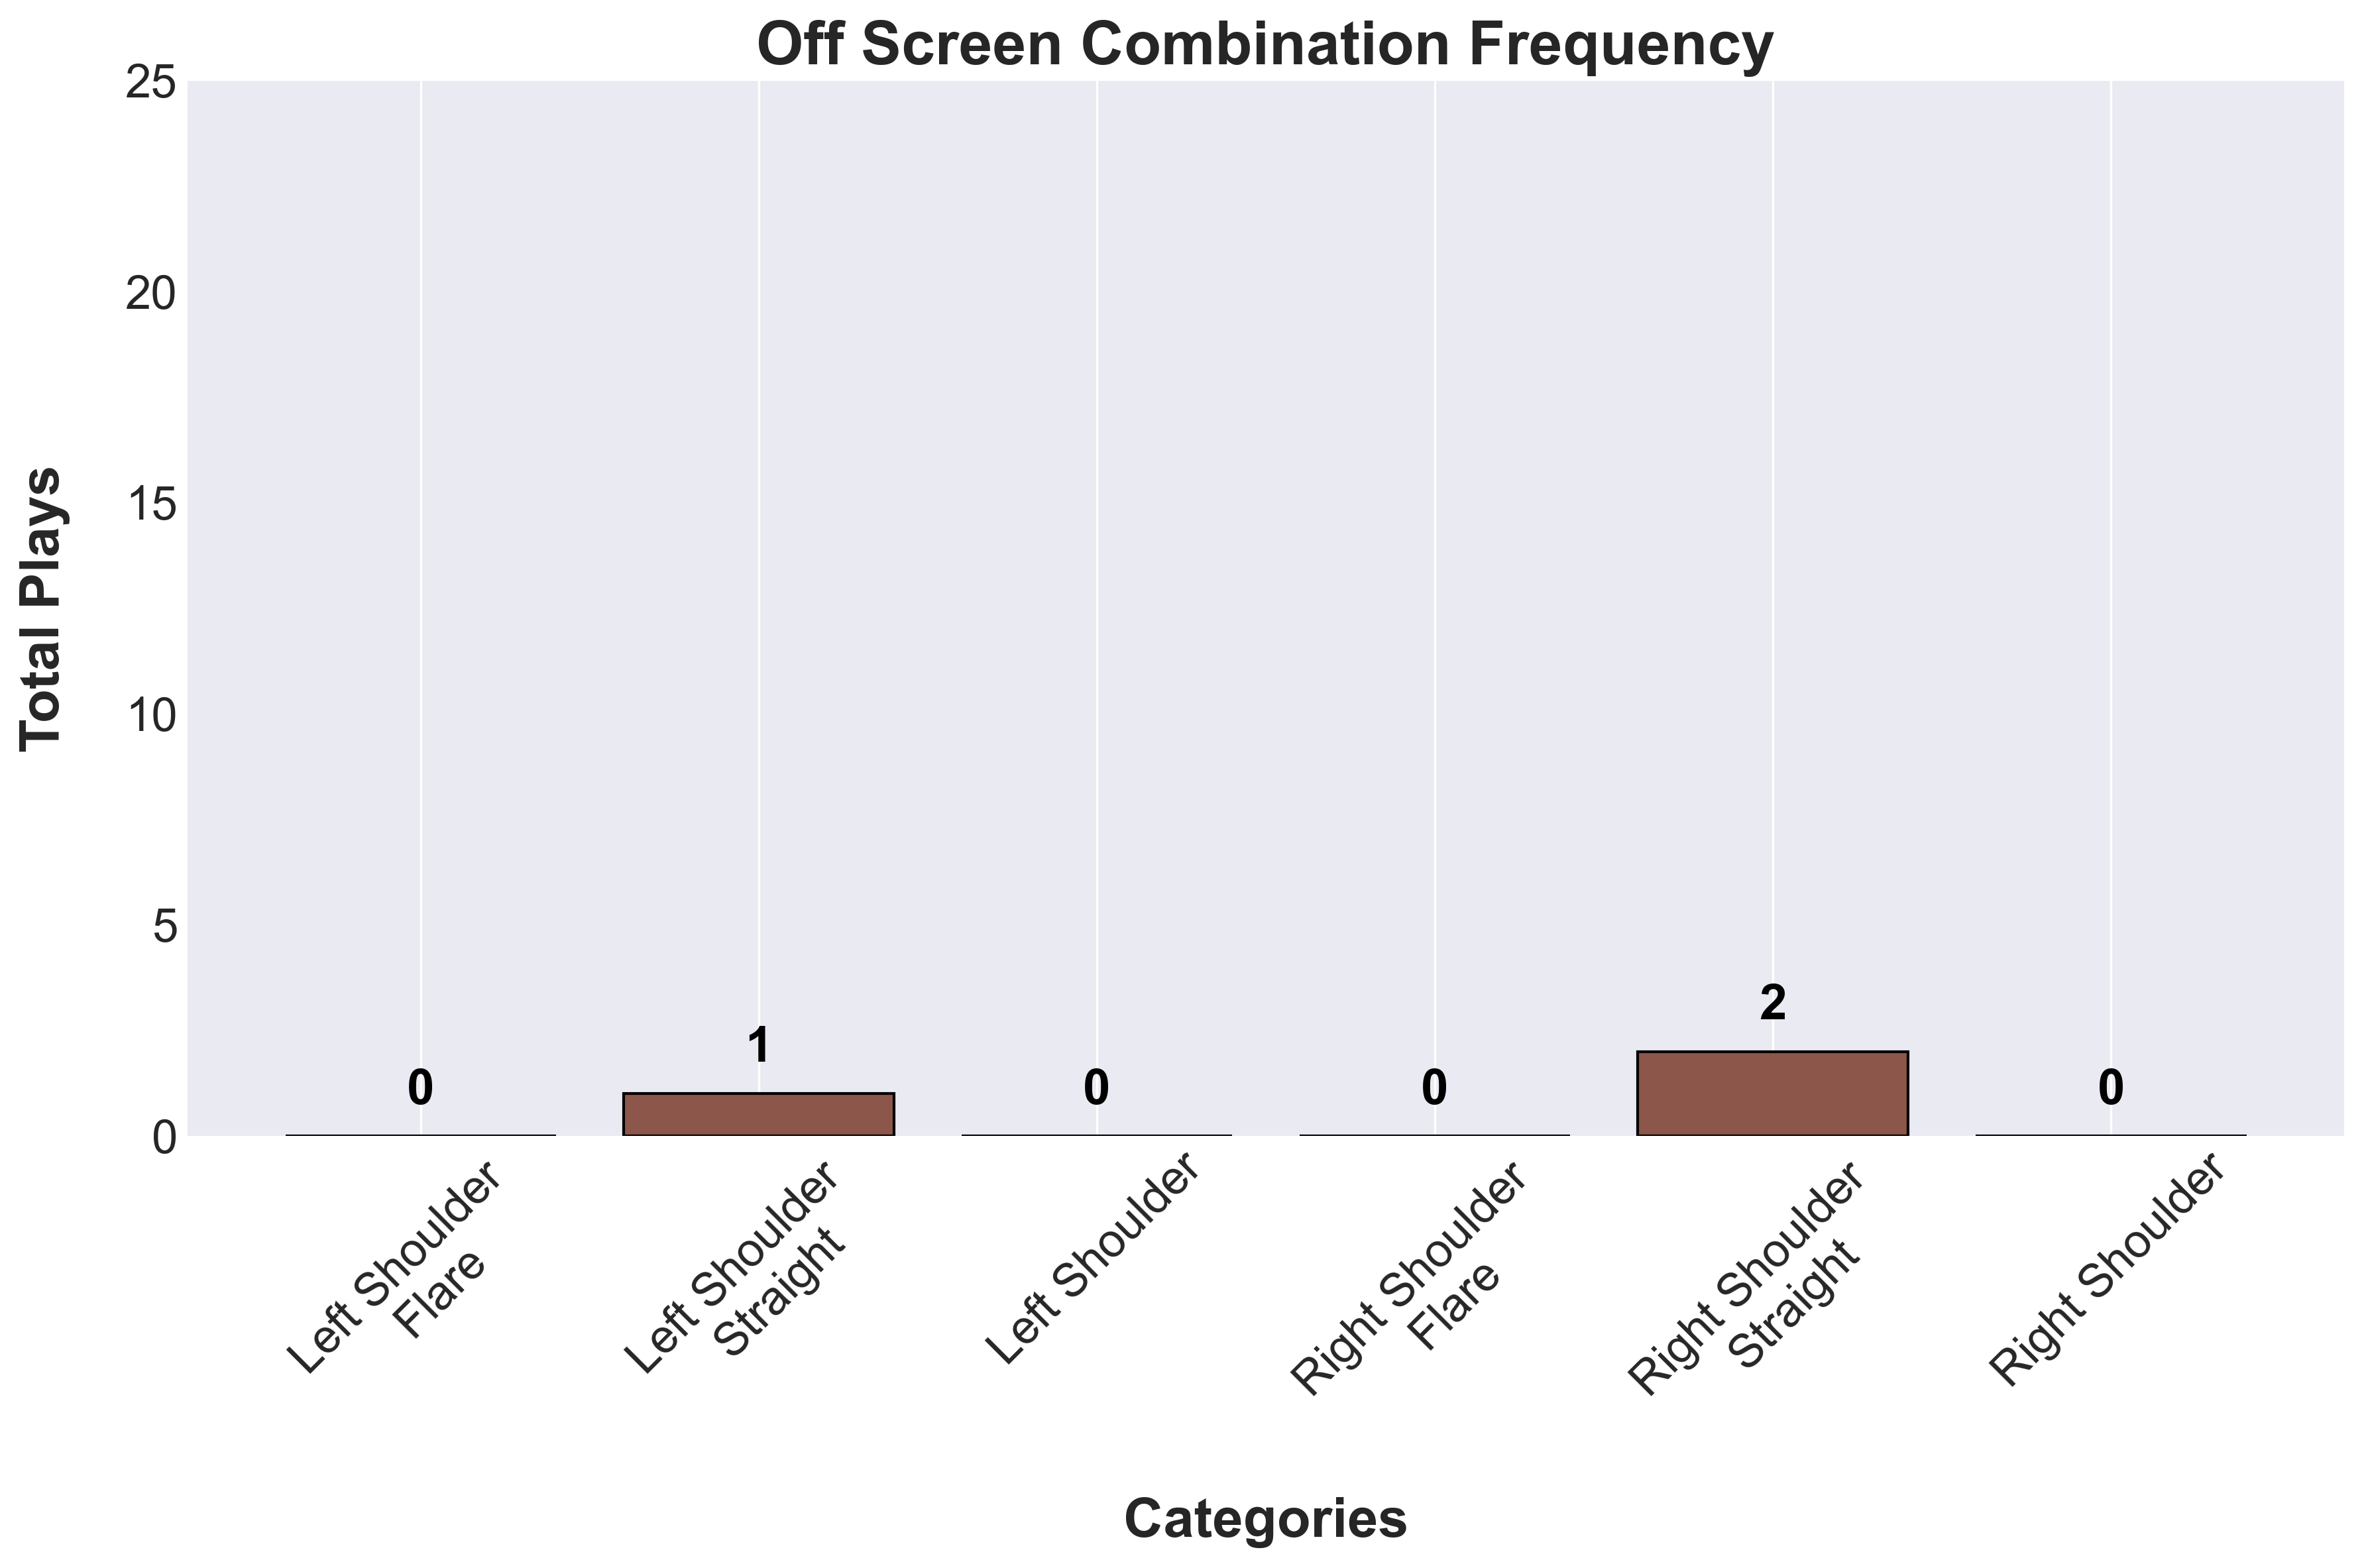
\includegraphics[width=\textwidth, height=.14\textheight]{images/OffScreen_Combination_Freq.png} % Adjust the width of the image to fit
    \end{minipage}
\end{table}

\vspace{-1em} % Add vertical space before the line (optional)
\hrule height 1pt width 1\textwidth % Adjust height and width
\vspace{1em} % Add vertical space after the line (optional)

\clearpage


% ----------------------
% Handoffs Visuals and Insights Section
% ----------------------
\subsection{Handoffs}
\begin{itemize}
    \item Opponent's handoff plays have a success rate of 60\%.
\end{itemize}

\vspace{1.25em} % Add vertical space before the line (optional)
\textbf{Key Notes on Handoff Tendencies}
\vspace{0.5em} % Add space between the title and the itemized list

\begin{itemize}
    \item Hand Offs make up x\% of players offensive load
    \vspace{0.3em} % Add space between the title and the itemized list
    \item Player is more likely to get pull up from 3 getting a handoff going left than going right
\end{itemize}

\vspace{1em} % Add vertical space before the line (optional)
\hrule height 1pt width 1\textwidth % Adjust height and width
\vspace{0em} % Add vertical space after the line (optional)

\subsubsection{Hand Off Shot Statistics}

% All Hand Off Statistics Table w/ room for insights
\begin{table}[H]
    \centering
    \begin{minipage}[t]{0.6\textwidth} % Left side (table) takes 85% of the width
        %\flushright
        \centering % Centering the title and the table
        \text{Total Hand Off Shot Statistics} % Title above the table in bold
        \vskip .25em % Adds vertical space between title and table
        \scalebox{.85}{ % Scale the entire table down by half
            \scriptsize % Reduce the font size
            \begin{tabular}{
            >{\centering\arraybackslash}p{.75cm} 
            >{\centering\arraybackslash}p{.5cm} 
            >{\centering\arraybackslash}p{.5cm} 
            >{\centering\arraybackslash}p{.5cm}
            >{\centering\arraybackslash}p{.5cm} 
            >{\centering\arraybackslash}p{.5cm} 
            >{\centering\arraybackslash}p{.5cm} 
            >{\centering\arraybackslash}p{.5cm}
            >{\centering\arraybackslash}p{.5cm} 
            >{\centering\arraybackslash}p{.5cm}
            >{\centering\arraybackslash}p{.5cm} 
            >{\centering\arraybackslash}p{.5cm}}% Adjust column widths
            \toprule
            \textbf{Plays} &
            \textbf{3PA} &
            \textbf{3PM} &
            \textbf{3P\%} & 
            \textbf{2PA} & 
            \textbf{2PM} & 
            \textbf{2P\%} & 
            \textbf{MiA} & 
            \textbf{MiM} &
            \textbf{Mi\%} &
            \textbf{TO} &
            \textbf{Foul} \\
            \midrule
            
                
                    18 & 2 & 1 &
                    50.0 & 
                    13 & 7 &
                    53.85 &
                    2 & 0 &
                    0.0 &
                    2 & 1 \\
                
            
                
            
                
            
                
            
                
            
                
            
                
            
                
            
                
            
                
            
                
            
                
            
                
            
                
            

            \bottomrule
            \end{tabular}
        }
    \end{minipage}
\end{table}

\vspace{0em} % Add vertical space before the line (optional)
%\hrule height 1pt width 1\textwidth % Adjust height and width
\vspace{-1em} % Add vertical space after the line (optional)

% Handoffs for shooting going Left vs Right
\begin{table}[H]
    \raisebox{3em}{ % Adjust this value to shift the tables vertically
    \begin{minipage}[t]{0.6\textwidth} % Left side (table) takes 85% of the width
        \flushleft
        \centering % Centering the title and the table
        \text{BH Hand Off Direction/Location Statistics} % Title above the table in bold
        \vskip .25em % Adds vertical space between title and table
        \scalebox{.6}{ % Scale the entire table down by half
            \renewcommand{\arraystretch}{1.4} % Adjust the number to increase or decrease row spacing
            \begin{tabular}{
            >{\centering\arraybackslash}p{1.75cm} 
            >{\centering\arraybackslash}p{.75cm} 
            >{\centering\arraybackslash}p{.75cm} 
            >{\centering\arraybackslash}p{.75cm} 
            >{\centering\arraybackslash}p{.75cm}
            >{\centering\arraybackslash}p{.75cm} 
            >{\centering\arraybackslash}p{.75cm} 
            >{\centering\arraybackslash}p{.75cm} 
            >{\centering\arraybackslash}p{.75cm}
            >{\centering\arraybackslash}p{.75cm} 
            >{\centering\arraybackslash}p{.75cm}
            >{\centering\arraybackslash}p{.75cm} 
            >{\centering\arraybackslash}p{.75cm}}% Adjust column widths
            \toprule
            {\scriptsize \textbf{PlayType}} &
            {\scriptsize \textbf{Plays}} &
            {\scriptsize \textbf{3PA}} &
            {\scriptsize \textbf{3PM}} &
            {\scriptsize \textbf{3P\%}} & 
            {\scriptsize \textbf{2PA}} & 
            {\scriptsize \textbf{2PM}} & 
            {\scriptsize \textbf{2P\%}} & 
            {\scriptsize \textbf{MiA}} & 
            {\scriptsize \textbf{MiM}} &
            {\scriptsize \textbf{Mi\%}} &
            {\scriptsize \textbf{TO}} &
            {\scriptsize \textbf{Foul}} \\
            \midrule
            
                
            
                
            
                
                    Left & 4 & 1 & 0 &
                    0.0 & 
                    3 & 1 &
                    33.33 &
                    1 & 0 &
                    0.0 &
                    0 & 0 \\
                
            
                
                    Right & 7 & 1 & 1 &
                    100.0 & 
                    5 & 3 &
                    60.0 &
                    1 & 0 &
                    0.0 &
                    1 & 0 \\
                
            
                
                    Top & 7 & 0 & 0 &
                    - & 
                    5 & 3 &
                    60.0 &
                    0 & 0 &
                    - &
                    1 & 1 \\
                
            
                
            
                
            
                
            
                
            
                
            
                
            
                
            
                
            
                
            

            \bottomrule
        \end{tabular}
        } % End of \scalebox
    \end{minipage}
    } % End of raisebox, closing the adjustment
    \hfill % This adds some flexible space between the table and the image
    \begin{minipage}[c]{0.35\textwidth} % Right side (image) takes 10% of the width
        \flushright
        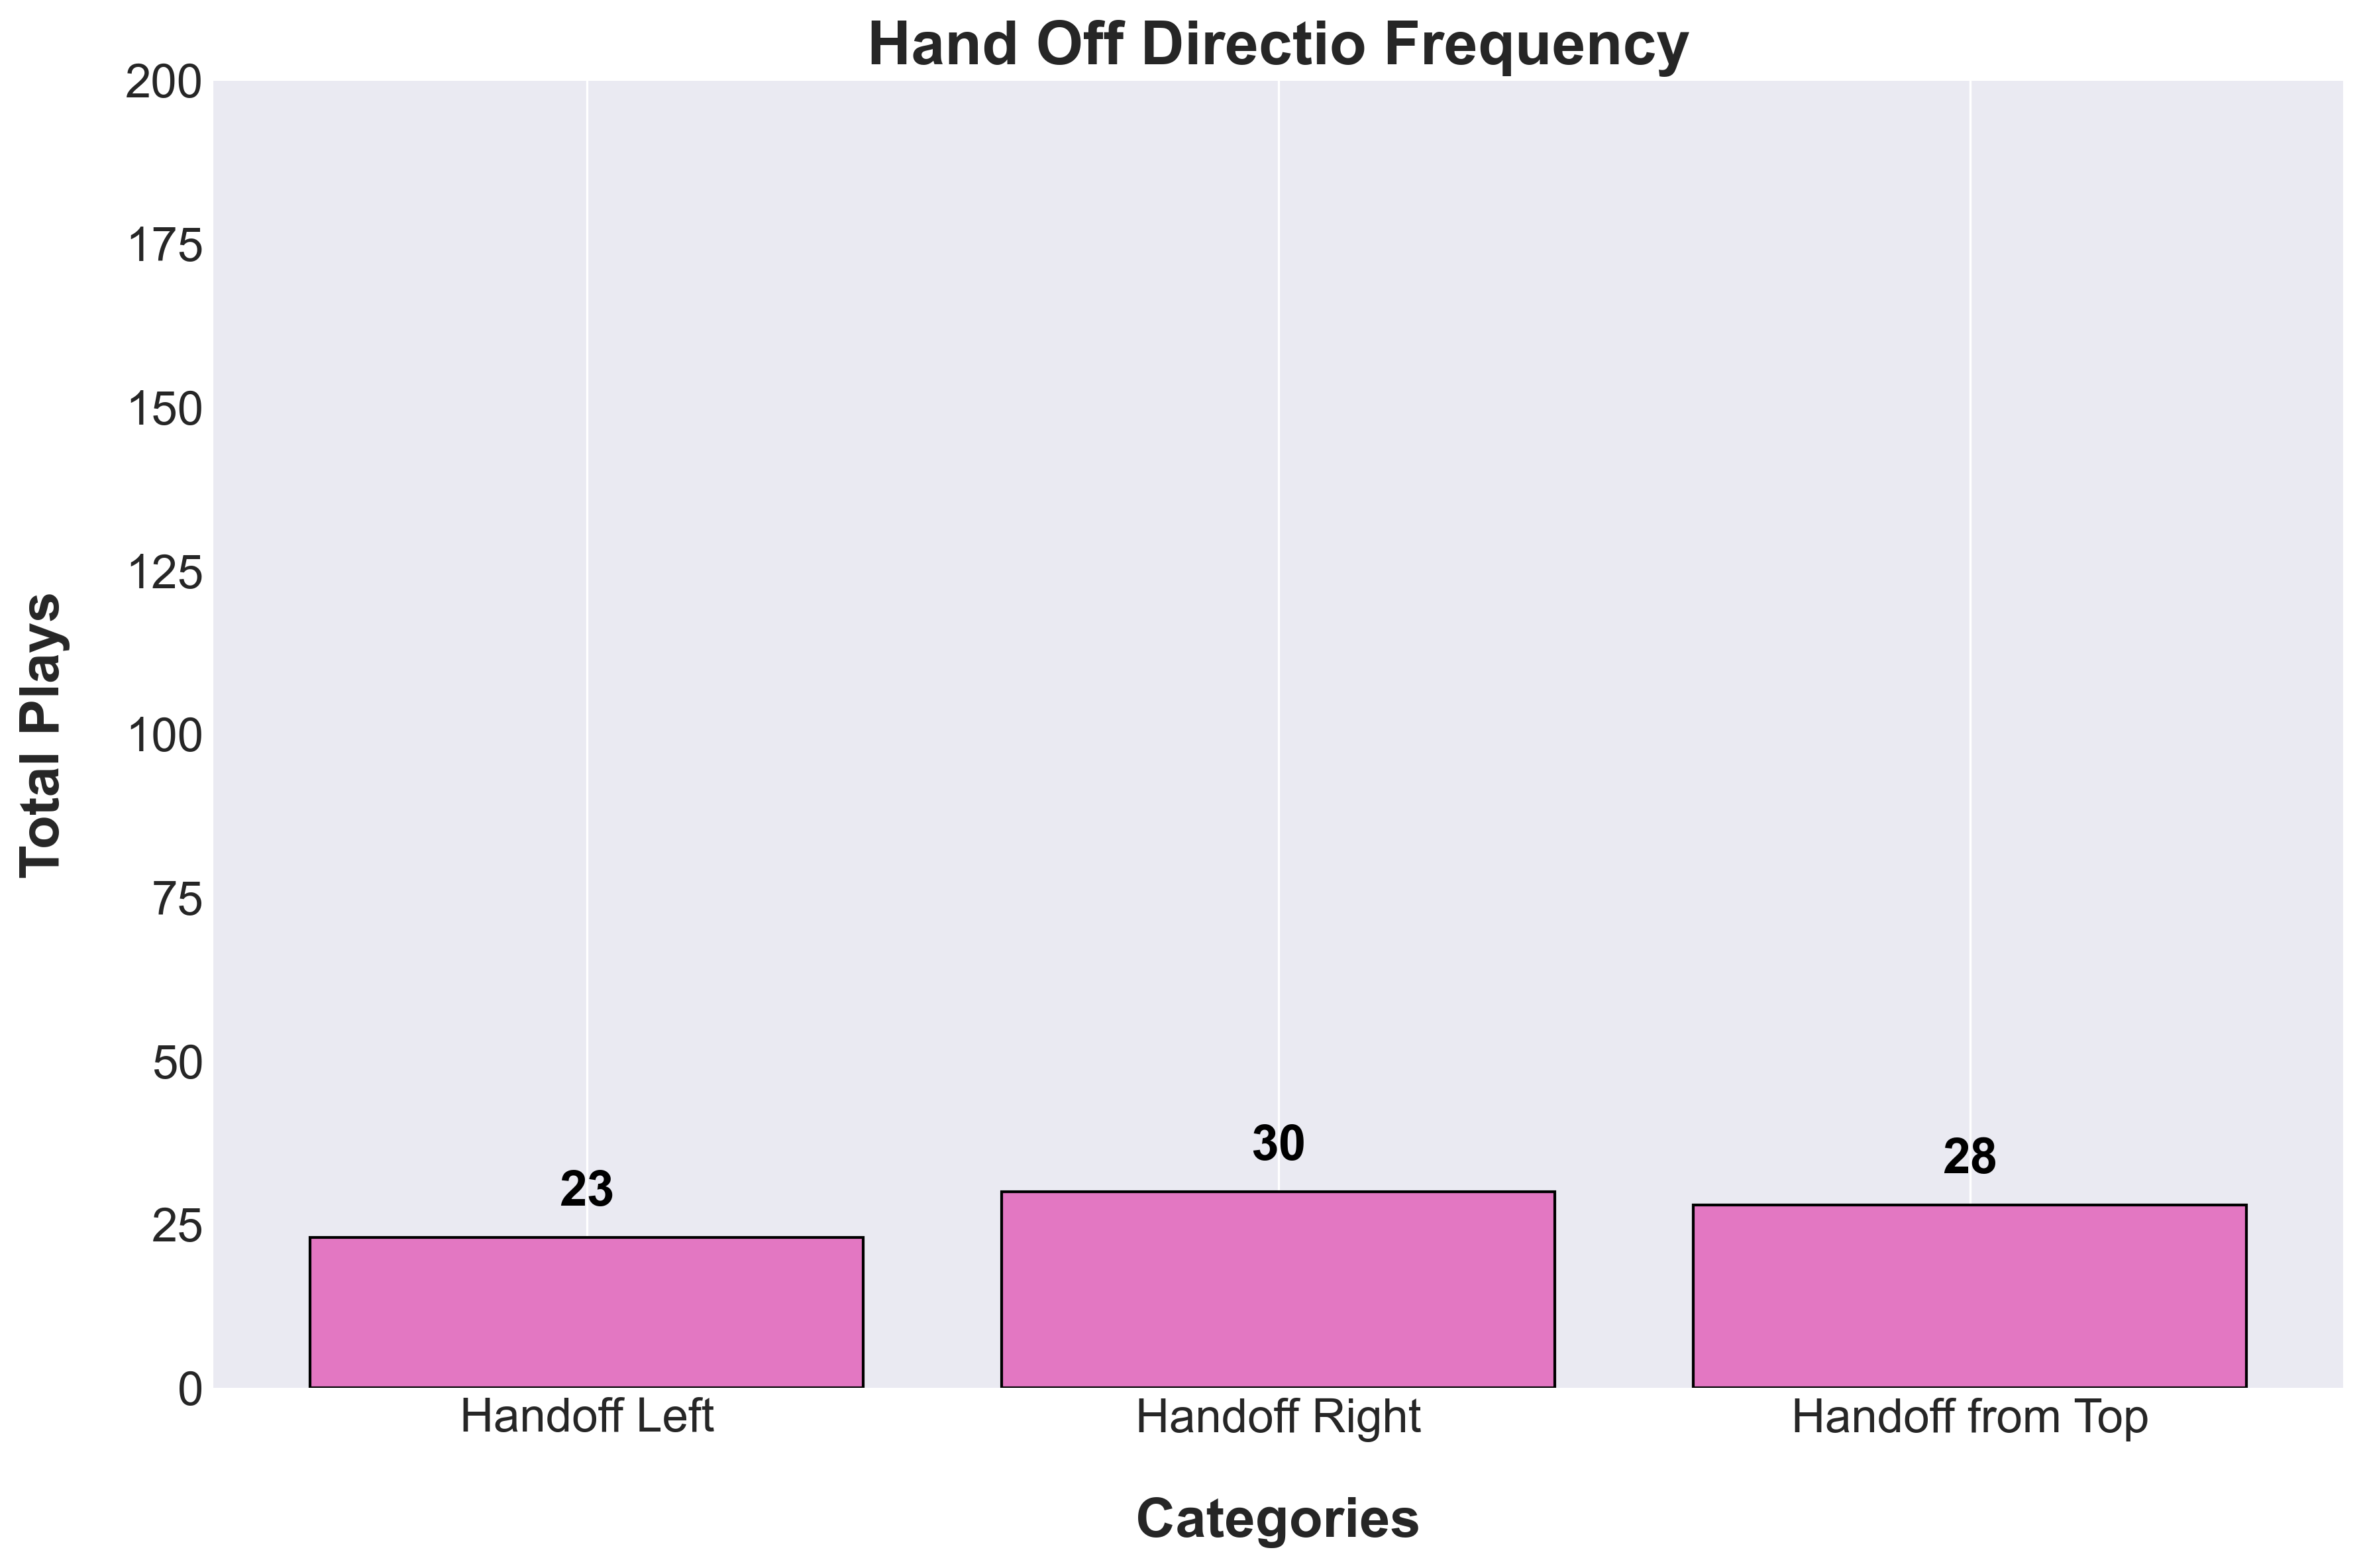
\includegraphics[width=\textwidth, height=.14\textheight]{images/HandOff_Direction_Freq.png} % Adjust the width of the image to fit
    \end{minipage}
\end{table}

\vspace{-1em} % Add vertical space before the line (optional)
%\hrule height 1pt width 1\textwidth % Adjust height and width
\vspace{-1em} % Add vertical space after the line (optional)

% Hand Off Type Statistics
\begin{table}[H]
    \raisebox{3.5em}{ % Adjust this value to shift the tables vertically
    \begin{minipage}[t]{0.6\textwidth} % Left side (table) takes 85% of the width
        \flushleft
        \centering % Centering the title and the table
        \text{Hand Off Type Statistics} % Title above the table in bold
        \vskip .25em % Adds vertical space between title and table
        \scalebox{.6}{ % Scale the entire table down by half
            \renewcommand{\arraystretch}{1.4} % Adjust the number to increase or decrease row spacing
            \begin{tabular}{
            >{\centering\arraybackslash}p{1.75cm} 
            >{\centering\arraybackslash}p{.75cm} 
            >{\centering\arraybackslash}p{.75cm} 
            >{\centering\arraybackslash}p{.75cm} 
            >{\centering\arraybackslash}p{.75cm}
            >{\centering\arraybackslash}p{.75cm} 
            >{\centering\arraybackslash}p{.75cm} 
            >{\centering\arraybackslash}p{.75cm} 
            >{\centering\arraybackslash}p{.75cm}
            >{\centering\arraybackslash}p{.75cm} 
            >{\centering\arraybackslash}p{.75cm}
            >{\centering\arraybackslash}p{.75cm} 
            >{\centering\arraybackslash}p{.75cm}}% Adjust column widths
            \toprule
            {\scriptsize \textbf{PlayType}} &
            {\scriptsize \textbf{Plays}} &
            {\scriptsize \textbf{3PA}} &
            {\scriptsize \textbf{3PM}} &
            {\scriptsize \textbf{3P\%}} & 
            {\scriptsize \textbf{2PA}} & 
            {\scriptsize \textbf{2PM}} & 
            {\scriptsize \textbf{2P\%}} & 
            {\scriptsize \textbf{MiA}} & 
            {\scriptsize \textbf{MiM}} &
            {\scriptsize \textbf{Mi\%}} &
            {\scriptsize \textbf{TO}} &
            {\scriptsize \textbf{Foul}} \\
            \midrule
            
                
            
                
            
                
            
                
            
                
            
                
            
                
                    Stationary & 5 & 0 & 0 &
                    - & 
                    4 & 3 &
                    75.0 &
                    0 & 0 &
                    - &
                    0 & 1 \\
                
            
                
                    Dribble & 13 & 2 & 1 &
                    50.0 & 
                    9 & 4 &
                    44.44 &
                    2 & 0 &
                    0.0 &
                    2 & 0 \\
                
            
                
            
                
            
                
            
                
            
                
            
                
            


            \bottomrule
        \end{tabular}
        } % End of \scalebox
    \end{minipage}
    } % End of raisebox, closing the adjustment
    \hfill
    \begin{minipage}[c]{0.35\textwidth} % Right side (image) takes 10% of the width
        \flushright
        \includegraphics[width=\textwidth, height=.14\textheight]{images/HandOff_Type_Freq.png} % Adjust the width of the image to fit
    \end{minipage}
    
\end{table}

\vspace{-1em} % Add vertical space before the line (optional)
%\hrule height 1pt width 1\textwidth % Adjust height and width
\vspace{-1em} % Add vertical space after the line (optional)

% Hand Off Stats for Combination of Direction and Type Stats
\begin{table}[H]
    \raisebox{4.5em}{ % Adjust this value to shift the tables vertically
    \begin{minipage}[t]{0.6\textwidth} % Left side (table) takes 85% of the width
        \flushleft
        \centering % Centering the title and the table
        \text{Hand Off Combination Statistics} % Title above the table in bold
        \vskip .25em % Adds vertical space between title and table
        \scalebox{.55}{ % Scale the entire table down by half
            \renewcommand{\arraystretch}{1.4} % Adjust the number to increase or decrease row spacing
            \begin{tabular}{
            >{\centering\arraybackslash}p{4cm} 
            >{\centering\arraybackslash}p{.75cm} 
            >{\centering\arraybackslash}p{.75cm} 
            >{\centering\arraybackslash}p{.75cm} 
            >{\centering\arraybackslash}p{.75cm}
            >{\centering\arraybackslash}p{.75cm} 
            >{\centering\arraybackslash}p{.75cm} 
            >{\centering\arraybackslash}p{.75cm} 
            >{\centering\arraybackslash}p{.75cm}
            >{\centering\arraybackslash}p{.75cm} 
            >{\centering\arraybackslash}p{.75cm}
            >{\centering\arraybackslash}p{.75cm} 
            >{\centering\arraybackslash}p{.75cm}}% Adjust column widths
            \toprule
            {\scriptsize \textbf{PlayType}} &
            {\scriptsize \textbf{Plays}} &
            {\scriptsize \textbf{3PA}} &
            {\scriptsize \textbf{3PM}} &
            {\scriptsize \textbf{3P\%}} & 
            {\scriptsize \textbf{2PA}} & 
            {\scriptsize \textbf{2PM}} & 
            {\scriptsize \textbf{2P\%}} & 
            {\scriptsize \textbf{MiA}} & 
            {\scriptsize \textbf{MiM}} &
            {\scriptsize \textbf{Mi\%}} &
            {\scriptsize \textbf{TO}} &
            {\scriptsize \textbf{Foul}} \\
            \midrule
            
                
            
                
            
                
            
                
            
                
            
                
            
                
            
                
            
                
            
                
                    Right - Stationary & 1 & 0 & 0 &
                    - & 
                    1 & 1 &
                    100.0 &
                    0 & 0 &
                    - &
                    0 & 0 \\
                
            
                
                    Top - Stationary & 4 & 0 & 0 &
                    - & 
                    3 & 2 &
                    66.67 &
                    0 & 0 &
                    - &
                    0 & 1 \\
                
            
                
                    Left - Dribble & 4 & 1 & 0 &
                    0.0 & 
                    3 & 1 &
                    33.33 &
                    1 & 0 &
                    0.0 &
                    0 & 0 \\
                
            
                
                    Right - Dribble & 6 & 1 & 1 &
                    100.0 & 
                    4 & 2 &
                    50.0 &
                    1 & 0 &
                    0.0 &
                    1 & 0 \\
                
            
                
                    Top - Dribble & 3 & 0 & 0 &
                    - & 
                    2 & 1 &
                    50.0 &
                    0 & 0 &
                    - &
                    1 & 0 \\
                
            


            \bottomrule
        \end{tabular}
        } % End of \scalebox
    \end{minipage}
    } % End of raisebox, closing the adjustment
    \hfill % This adds some flexible space between the table and the image
    \begin{minipage}[c]{0.35\textwidth} % Right side (image) takes 10% of the width
        \flushright
        \includegraphics[width=\textwidth, height=.14\textheight]{images/HandOff_Combination_Freq.png} % Adjust the width of the image to fit
    \end{minipage}
\end{table}

\vspace{-1em} % Add vertical space before the line (optional)
\hrule height 1pt width 1\textwidth % Adjust height and width
\vspace{1em} % Add vertical space after the line (optional)

\clearpage


% ----------------------
% Iso Visuals and Insights Section
% ----------------------
\subsection{Iso}
\vspace{0.25em} % Add vertical space before the line (optional)
\textbf{Key Notes on Iso Tendencies}
\vspace{0.5em} % Add space between the title and the itemized list

\begin{itemize}
    \item Iso Plays make up x\% of players offensive load
    \vspace{0.3em} % Add space between the title and the itemized list
    \item Player is in the 35\% in scoring efficiency off cuts in the liberty league.
\end{itemize}

\vspace{1em} % Add vertical space after the line (optional)
\hrule height 1pt width 1\textwidth % Adjust height and width
\vspace{0em} % Add vertical space after the line (optional)

\subsubsection{General Iso Stats}
% All Cutter Statistics Table w/ room for insights
\begin{table}[H]
    \centering
    \begin{minipage}[t]{0.6\textwidth} % Left side (table) takes 85% of the width
        %\flushright
        \centering % Centering the title and the table
        \text{Total Iso Statistics} % Title above the table in bold
        \vskip .25em % Adds vertical space between title and table
        \scalebox{.85}{ % Scale the entire table down by half
            \scriptsize % Reduce the font size
            \begin{tabular}{
            >{\centering\arraybackslash}p{.75cm} 
            >{\centering\arraybackslash}p{.5cm} 
            >{\centering\arraybackslash}p{.5cm} 
            >{\centering\arraybackslash}p{.5cm}
            >{\centering\arraybackslash}p{.5cm} 
            >{\centering\arraybackslash}p{.5cm} 
            >{\centering\arraybackslash}p{.5cm} 
            >{\centering\arraybackslash}p{.5cm}
            >{\centering\arraybackslash}p{.5cm} 
            >{\centering\arraybackslash}p{.5cm}
            >{\centering\arraybackslash}p{.5cm} 
            >{\centering\arraybackslash}p{.5cm}}% Adjust column widths
            \toprule
            \textbf{Plays} &
            \textbf{3PA} &
            \textbf{3PM} &
            \textbf{3P\%} & 
            \textbf{2PA} & 
            \textbf{2PM} & 
            \textbf{2P\%} & 
            \textbf{MiA} & 
            \textbf{MiM} &
            \textbf{Mi\%} &
            \textbf{TO} &
            \textbf{Foul} \\
            \midrule
            
                
            
                
            
                
            
                
            
                
            
                
                    19 & 0 & 0 &
                    - & 
                    14 & 7 &
                    50.0 &
                    4 & 3 &
                    75.0 &
                    1 & 4 \\
                
            
                
            
                
            
                
            
                
            


            \bottomrule
            \end{tabular}
        }
    \end{minipage}
\end{table}

\vspace{0em} % Add vertical space before the line (optional)
%\hrule height 1pt width 1\textwidth % Adjust height and width
\vspace{-1em} % Add vertical space after the line (optional)

% Iso Stats for Top vs Right vs Left 
\begin{table}[H]
    \raisebox{3em}{ % Adjust this value to shift the tables vertically
    \begin{minipage}[t]{0.6\textwidth} % Left side (table) takes 85% of the width
        \flushleft
        \centering % Centering the title and the table
        \text{Iso Direction/Location Statistics} % Title above the table in bold
        \vskip .25em % Adds vertical space between title and table
        \scalebox{.6}{ % Scale the entire table down by half
            \renewcommand{\arraystretch}{1.4} % Adjust the number to increase or decrease row spacing
            \begin{tabular}{
            >{\centering\arraybackslash}p{1.75cm} 
            >{\centering\arraybackslash}p{.75cm} 
            >{\centering\arraybackslash}p{.75cm} 
            >{\centering\arraybackslash}p{.75cm} 
            >{\centering\arraybackslash}p{.75cm}
            >{\centering\arraybackslash}p{.75cm} 
            >{\centering\arraybackslash}p{.75cm} 
            >{\centering\arraybackslash}p{.75cm} 
            >{\centering\arraybackslash}p{.75cm}
            >{\centering\arraybackslash}p{.75cm} 
            >{\centering\arraybackslash}p{.75cm}
            >{\centering\arraybackslash}p{.75cm} 
            >{\centering\arraybackslash}p{.75cm}}% Adjust column widths
            \toprule
            {\scriptsize \textbf{PlayType}} &
            {\scriptsize \textbf{Plays}} &
            {\scriptsize \textbf{3PA}} &
            {\scriptsize \textbf{3PM}} &
            {\scriptsize \textbf{3P\%}} & 
            {\scriptsize \textbf{2PA}} & 
            {\scriptsize \textbf{2PM}} & 
            {\scriptsize \textbf{2P\%}} & 
            {\scriptsize \textbf{MiA}} & 
            {\scriptsize \textbf{MiM}} &
            {\scriptsize \textbf{Mi\%}} &
            {\scriptsize \textbf{TO}} &
            {\scriptsize \textbf{Foul}} \\
            \midrule
            
                
            
                
            
                
            
                
            
                
            
                
            
                
            
                
                    Left & 4 & 0 & 0 &
                    - & 
                    3 & 2 &
                    66.67 &
                    1 & 1 &
                    100.0 &
                    0 & 1 \\
                
            
                
                    Right & 8 & 0 & 0 &
                    - & 
                    5 & 3 &
                    60.0 &
                    2 & 1 &
                    50.0 &
                    1 & 2 \\
                
            
                
                    Top & 7 & 0 & 0 &
                    - & 
                    6 & 2 &
                    33.33 &
                    1 & 1 &
                    100.0 &
                    0 & 1 \\
                
            


            \bottomrule
        \end{tabular}
        } % End of \scalebox
    \end{minipage}
    } % End of raisebox, closing the adjustment
    \hfill % This adds some flexible space between the table and the image
    \begin{minipage}[c]{0.35\textwidth} % Right side (image) takes 10% of the width
        \flushright
        \includegraphics[width=\textwidth, height=.14\textheight]{images/IsoDirectionLocation_Freq.png} % Adjust the width of the image to fit
    \end{minipage}
\end{table}

\vspace{0em} % Add vertical space before the line (optional)
\hrule height 1pt width 1\textwidth % Adjust height and width
\vspace{1em} % Add vertical space after the line (optional)

\clearpage



% ----------------------
% Cutter Visuals and Insights Section
% ----------------------
\subsection{Cuts}
\vspace{0.25em} % Add vertical space before the line (optional)
\textbf{Key Notes on Cutter Tendencies}
\vspace{0.5em} % Add space between the title and the itemized list

\begin{itemize}
    \item Cutting Plays make up 100\% of players offensive load
    \vspace{0.3em} % Add space between the title and the itemized list
    \item Player is in the - in scoring efficiency off cuts in the liberty league.
\end{itemize}

\vspace{1em} % Add vertical space after the line (optional)
\hrule height 1pt width 1\textwidth % Adjust height and width
\vspace{0em} % Add vertical space after the line (optional)

\subsubsection{General Cutter Stats}
% All Cutter Statistics Table w/ room for insights
\begin{table}[H]
    \centering
    \begin{minipage}[t]{0.6\textwidth} % Left side (table) takes 60% of the width
        \centering % Centering the title and the table
        \textbf{Total Cutter Statistics} % Title above the table in bold
        \vskip .25em % Adds vertical space between title and table
        \scalebox{.85}{ % Scale the entire table down by 85%
            \scriptsize % Reduce the font size
            \begin{tabular}{
            >{\centering\arraybackslash}p{.75cm} 
            >{\centering\arraybackslash}p{.5cm} 
            >{\centering\arraybackslash}p{.5cm} 
            >{\centering\arraybackslash}p{.5cm}
            >{\centering\arraybackslash}p{.5cm} 
            >{\centering\arraybackslash}p{.5cm} 
            >{\centering\arraybackslash}p{.5cm} 
            >{\centering\arraybackslash}p{.5cm}
            >{\centering\arraybackslash}p{.5cm} 
            >{\centering\arraybackslash}p{.5cm}
            >{\centering\arraybackslash}p{.5cm} 
            >{\centering\arraybackslash}p{.5cm}}% Adjust column widths
            \toprule
            \textbf{Plays} &
            \textbf{3PA} &
            \textbf{3PM} &
            \textbf{3P\%} & 
            \textbf{2PA} & 
            \textbf{2PM} & 
            \textbf{2P\%} & 
            \textbf{MiA} & 
            \textbf{MiM} &
            \textbf{Mi\%} &
            \textbf{TO} &
            \textbf{Foul} \\
            \midrule
            
                
            
                
            
                
            
                
            
                
            
                
                    9 & 0 &
                    0 & - & 
                    8 & 7 &
                    87.5 &
                    0 & 0 &
                    - &
                    1 & 0 \\ 
                
            
                
            
                
            
                
            
                
            
            \bottomrule
            \end{tabular}
        }
    \end{minipage}
\end{table}

\vspace{0em} % Add vertical space before the line (optional)
%\hrule height 1pt width 1\textwidth % Adjust height and width
\vspace{-1em} % Add vertical space after the line (optional)

% Cutter Stats for Basket vs Flash vs Screen Cuts 
\begin{table}[H]
    \raisebox{3em}{ % Adjust this value to shift the tables vertically
    \begin{minipage}[t]{0.6\textwidth} % Left side (table) takes 60% of the width
        \flushleft
        \centering % Centering the title and the table
        \textbf{Cut Type Statistics} % Title above the table in bold
        \vskip .25em % Adds vertical space between title and table
        \scalebox{.6}{ % Scale the entire table down by 60%
            \renewcommand{\arraystretch}{1.4} % Adjust the number to increase or decrease row spacing
            \begin{tabular}{
            >{\centering\arraybackslash}p{1.75cm} 
            >{\centering\arraybackslash}p{.75cm} 
            >{\centering\arraybackslash}p{.75cm} 
            >{\centering\arraybackslash}p{.75cm} 
            >{\centering\arraybackslash}p{.75cm}
            >{\centering\arraybackslash}p{.75cm} 
            >{\centering\arraybackslash}p{.75cm} 
            >{\centering\arraybackslash}p{.75cm} 
            >{\centering\arraybackslash}p{.75cm}
            >{\centering\arraybackslash}p{.75cm} 
            >{\centering\arraybackslash}p{.75cm}
            >{\centering\arraybackslash}p{.75cm} 
            >{\centering\arraybackslash}p{.75cm}}% Adjust column widths
            \toprule
            {\scriptsize \textbf{PlayType}} &
            {\scriptsize \textbf{Plays}} &
            {\scriptsize \textbf{3PA}} &
            {\scriptsize \textbf{3PM}} &
            {\scriptsize \textbf{3P\%}} & 
            {\scriptsize \textbf{2PA}} & 
            {\scriptsize \textbf{2PM}} & 
            {\scriptsize \textbf{2P\%}} & 
            {\scriptsize \textbf{MiA}} & 
            {\scriptsize \textbf{MiM}} &
            {\scriptsize \textbf{Mi\%}} &
            {\scriptsize \textbf{TO}} &
            {\scriptsize \textbf{Foul}} \\
            \midrule
            
                
            
                
            
                
            
                
            
                
            
                
            
                
            
                
                    Basket & 7 & 0 &
                    0 & - & 
                    6 & 5 &
                    83.33 &
                    0 & 0 &
                    - &
                    1 & 0 \\
                
            
                        
                    Flash & 2 & 0 &
                    0 & - & 
                    2 & 2 &
                    100.0 &
                    0 & 0 &
                    - &
                    0 & 0 \\
                
            
                
            


            \bottomrule
        \end{tabular}
        } % End of \scalebox
    \end{minipage}
    } % End of raisebox, closing the adjustment
    \hfill % This adds some flexible space between the table and the image
    \begin{minipage}[c]{0.35\textwidth} % Right side (image) takes 35% of the width
        \flushright
        \includegraphics[width=\textwidth, height=.14\textheight]{images/Cut_Type_Freq.png} % Adjust the width of the image to fit
    \end{minipage}
\end{table}

\vspace{0em} % Add vertical space before the line (optional)
%\hrule height 1pt width 1\textwidth % Adjust height and width
\vspace{-1em} % Add vertical space after the line (optional)

\clearpage





% ----------------------
% Transition Visuals and Insights Section
% ----------------------
\subsection{Transition}
\vspace{0.25em} % Add vertical space before the line (optional)
\textbf{Key Notes on Iso Tendencies}
\vspace{0.5em} % Add space between the title and the itemized list

\begin{itemize}
    \item Transition Plays make up x\% of players offensive load
    \vspace{0.3em} % Add space between the title and the itemized list
    \item More Specifically, player is much more efficient getting out to left wing in transition vs the right wing in transition. 
\end{itemize}

\vspace{1em} % Add vertical space after the line (optional)
\hrule height 1pt width 1\textwidth % Adjust height and width
\vspace{0em} % Add vertical space after the line (optional)

\subsubsection{General Transition Stats}
% All Cutter Statistics Table w/ room for insights
\begin{table}[H]
    \centering
    \begin{minipage}[t]{0.6\textwidth} % Left side (table) takes 85% of the width
        %\flushright
        \centering % Centering the title and the table
        \text{Total Transition Statistics} % Title above the table in bold
        \vskip .25em % Adds vertical space between title and table
        \scalebox{.85}{ % Scale the entire table down by half
            \scriptsize % Reduce the font size
            \begin{tabular}{
            >{\centering\arraybackslash}p{.75cm} 
            >{\centering\arraybackslash}p{.5cm} 
            >{\centering\arraybackslash}p{.5cm} 
            >{\centering\arraybackslash}p{.5cm}
            >{\centering\arraybackslash}p{.5cm} 
            >{\centering\arraybackslash}p{.5cm} 
            >{\centering\arraybackslash}p{.5cm} 
            >{\centering\arraybackslash}p{.5cm}
            >{\centering\arraybackslash}p{.5cm} 
            >{\centering\arraybackslash}p{.5cm}
            >{\centering\arraybackslash}p{.5cm} 
            >{\centering\arraybackslash}p{.5cm}}% Adjust column widths
            \toprule
            \textbf{Plays} &
            \textbf{3PA} &
            \textbf{3PM} &
            \textbf{3P\%} & 
            \textbf{2PA} & 
            \textbf{2PM} & 
            \textbf{2P\%} & 
            \textbf{MiA} & 
            \textbf{MiM} &
            \textbf{Mi\%} &
            \textbf{TO} &
            \textbf{Foul} \\
            \midrule
            
                
            
                
                    73 & 9 & 3 &
                    37.5 & 
                    37 & 22 &
                    75.11 &
                    7 & 4 &
                    66.67 &
                    15 & 11 \\
                
            
                
            
                
            
                
            
                
            
                
            


            \bottomrule
            \end{tabular}
        }
    \end{minipage}
\end{table}

\vspace{0em} % Add vertical space before the line (optional)
%\hrule height 1pt width 1\textwidth % Adjust height and width
\vspace{-1em} % Add vertical space after the line (optional)

% Transition Stats for BH vs Leakouts vs Left Wing vs Right Wing vs Trailer
\begin{table}[H]
    \raisebox{4.5em}{ % Adjust this value to shift the tables vertically
    \begin{minipage}[t]{0.6\textwidth} % Left side (table) takes 85% of the width
        \flushleft
        \centering % Centering the title and the table
        \text{Transition Type Statistics} % Title above the table in bold
        \vskip .25em % Adds vertical space between title and table
        \scalebox{.58}{ % Scale the entire table down by half
            \renewcommand{\arraystretch}{1.4} % Adjust the number to increase or decrease row spacing
            \begin{tabular}{
            >{\centering\arraybackslash}p{2.5cm} 
            >{\centering\arraybackslash}p{.75cm} 
            >{\centering\arraybackslash}p{.75cm} 
            >{\centering\arraybackslash}p{.75cm} 
            >{\centering\arraybackslash}p{.75cm}
            >{\centering\arraybackslash}p{.75cm} 
            >{\centering\arraybackslash}p{.75cm} 
            >{\centering\arraybackslash}p{.75cm} 
            >{\centering\arraybackslash}p{.75cm}
            >{\centering\arraybackslash}p{.75cm} 
            >{\centering\arraybackslash}p{.75cm}
            >{\centering\arraybackslash}p{.75cm}
            >{\centering\arraybackslash}p{.75cm}}% Adjust column widths
            \toprule
            {\scriptsize \textbf{PlayType}} &
            {\scriptsize \textbf{Plays}} &
            {\scriptsize \textbf{3PA}} &
            {\scriptsize \textbf{3PM}} &
            {\scriptsize \textbf{3P\%}} & 
            {\scriptsize \textbf{2PA}} & 
            {\scriptsize \textbf{2PM}} & 
            {\scriptsize \textbf{2P\%}} & 
            {\scriptsize \textbf{MiA}} & 
            {\scriptsize \textbf{MiM}} &
            {\scriptsize \textbf{Mi\%}} &
            {\scriptsize \textbf{TO}} &
            {\scriptsize \textbf{Foul}} \\
            \midrule
            
                
            
                
            
                
                    BH & 42 & 1 & 0 &
                    0.0 & 
                    20 & 11 &
                    55.0 &
                    4 & 2 &
                     &
                    11 & 10 \\
                
            
                
                    Leakouts & 3 & 0 & 0 &
                    - & 
                    2 & 2 &
                    100.0 &
                    0 & 0 &
                    - &
                    0 & 0 \\
                
            
                
                    Left Wing & 16 & 1 & 1 &
                    100.0 & 
                    11 & 5 &
                    45.45 &
                    2 & 1 &
                    50.0 &
                    3 & 1 \\
                
            
                
                    Right Wing & 8 & 3 & 0 &
                    0.0 & 
                    4 & 4 &
                    100.0 &
                    1 & 1 &
                    100.0 &
                    1 & 0 \\
                
            
                
                    Trailer & 4 & 4 & 2 &
                    50.0 & 
                    0 & 0 &
                    - &
                    0 & 0 &
                    - &
                    0 & 0 \\
                
            


            \bottomrule
        \end{tabular}
        } % End of \scalebox
    \end{minipage}
    } % End of raisebox, closing the adjustment
    \hfill % This adds some flexible space between the table and the image
    \begin{minipage}[c]{0.35\textwidth} % Right side (image) takes 10% of the width
        \flushright
        \includegraphics[width=\textwidth, height=.14\textheight]{images/Transition_Type_Freq.png} % Adjust the width of the image to fit
    \end{minipage}
\end{table}

\vspace{0em} % Add vertical space before the line (optional)
\hrule height 1pt width 1\textwidth % Adjust height and width
\vspace{1em} % Add vertical space after the line (optional)

\clearpage


%---------------------------------
% Data Disclaimers
%---------------------------------
\section*{Data Disclaimers}

\vspace{0.5cm} % Adds vertical space between items

\begin{itemize}[leftmargin=*, label=\textbf{•}]
    \item \textbf{Legal Data Collection:} All data presented in this document was legally scraped from Synergy using a program developed by Kyle Krebs.
    
    \vspace{0.3cm} % Adds vertical space between items

    \item \textbf{Purpose of Report:} This report aims to offer detailed insights into specific player statistics, facilitating players and coaches in comprehensively understanding the behavioral patterns of their opponents.

    \vspace{0.3cm} % Adds vertical space between items
    
    \item \textbf{Use of Report:} This report is intended to demonstrate my skills in data analysis and report generation. Please note that all personal names and team names have been anonymized to protect privacy and maintain confidentiality when showing 3rd parties.
    
    \vspace{0.3cm}
    
    \item \textbf{Data Accuracy:} While efforts have been made to ensure the accuracy of the data, there may still be some errors in the numbers. If you identify any discrepancies, please feel free to reach out to me.
    
    \vspace{0.3cm}
    
    \item \textbf{Permission Granted:} I have received permission from coaches to use and analyze data that has been scraped from Synergy.
    
    \vspace{0.3cm}
    
    \item \textbf{Content Generation:} All content generated in the following report was created by Kyle Krebs.
\end{itemize}

\vspace{0cm} % Adds space before the contact section

\subsubsection*{Contact Information}

For questions or concerns regarding this report or data privacy, please contact:

\begin{itemize}[leftmargin=*, label={}]
    \item \textbf{Kyle Krebs}
    \item \textbf{Email:} \href{mailto:kak4294@rit.edu}{kak4294@rit.edu}
    \item \textbf{Phone:} 845-418-9959
\end{itemize}


\vspace{1.5em}

\small
\section*{General Stat Information \& Statistic Definitions}

    \vspace{1em}
    \noindent \textbf{!! IMPORTANT PLEASE READ !!} All statistics measured in this report were actions that had ended in either a shot taken, foul drawn, or turnover. With this information we are able to intrepet where players get their shots from. This doesn't track total amount of times a player does a specific action, it only tracks when those actions end in the way I said above. 
    \vspace{1em}
    
    \noindent \textbf{Offensive Load:} Measures the total number of offensive actions a player performs, including shots taken, fouls drawn, and turnovers.
    
    \noindent \textbf{Efficiency:} Measured by a players performance of their 3pt\%, 2pt\%, Midrange\%, Turnovers, and Fouls Drawn

\vspace{.3em}


    
\subsection*{Pick-and-Roll}

    \noindent \textbf{Usage:} Determines whether a player goes off a screen or rejects it.
    
    \noindent \textbf{Direction/Location:} Direction pertains to the stats in the 'Left' / 'Right' rows as they give us the direction the ball handler is going. Location pertains to the stats in the 'High' row as it tells us the screen occurs when the screener is completely outside the 3 point line. Direction is unknown in High pick-and-rolls.
    
    \noindent \textbf{PNR to Different Playtypes:} Each row pertains to another action to which the ball handler had passed it to another player out of the pick-and-roll that proceeded to execute the given action.

\vspace{.5em}

\subsection*{Post Ups}

    \noindent \textbf{Location:} Pertains to the spot of the floor where the player had started his post up. 
    
    \noindent \textbf{Shot Type:} Tells us which shoulder the player had shot over, or if the player faced up on the post up. 
    
    \noindent \textbf{Post to Different Playtypes:} Each table pertains to another action to which the post player had passed it to another player out of the post that proceeded to execute the given action.

\vspace{.5em}

\subsection*{Rollman}

    \noindent \textbf{Play Type:} Represents whether the Rollman popped, slipped, or rolled to basket after screen.
    
    \noindent \textbf{Slip to Drive:} Goes over direction that player drove after slipping a screen and driving

     \noindent \textbf{Pop to Drive:} Goes over direction that player drove after popping and driving

\vspace{.5em}


\subsection*{Spot Ups}

    \noindent \textbf{Jumpshots:} Defined as a catch and shoot jump shot received from a pass of a teammate. 
    
    \noindent \textbf{Drives:} Defined as when someone catches the ball on the outside of the 3 point line and took at least one dribble to get a shot/turnover of some sort.
    
    \noindent \textbf{Drive Direction:} Defined as the which way the player had dribbled the ball after catching the pass in a spot up position.
    
    \noindent \textbf{Different Playtype to Jumpshot/Drive:} Pertains to an action that a player in a spot up position receives a pass from. 

\vspace{.5em}

\subsection*{Off Screens}

    \noindent \textbf{Running off Specific Shoulder:} Refers to the shoulder that the shooter hits the screener with when running off a screen. 
    
    \noindent \textbf{Type:} Refers to one of three options, \underline{Flare}: when someone sets a screen away from the player with the ball to help a teammate get open for a shot or move. \underline{Curl}: when a player comes off a screen and catches the ball going directly to the basket. \underline{Straight}: when a player runs directly off a screen to catch the ball at the three point line. 

\vspace{.5em}


\subsection*{Handoffs}

    \noindent \textbf{Direction/Location:} Direction refers to 'Left' / 'Right' rows, where the shooter receives the hand offs moving in the given direction. Location refers to the 'Top' row where direction is not specified, yet the location of the hand off happens at the center of the court above the 3 point line. 
    
    \noindent \textbf{Type:} Refers to what the person handing the ball off is doing when the shooter receives the hand off. \underline{Stationary}: staying in one spot. \underline{Dribble}: continuously dribbling towards shooter in hand off.

\vspace{.5em}

\subsection*{Iso}

    \noindent \textbf{Location:} Refers to where on the court the isolation occurs. \underline{Left} refers to left wing and left corner. \underline{Right} refers to right wing and right corner. \underline{Top} refers to center of the court above the three point line.

\vspace{.5em}

\subsection*{Cuts}

    \noindent \textbf{Type:} Refers to one of three options. \underline{Basket}: when a player gets a pass running towards the basket. \underline{Flash}: when a player catches a pass running towards an open space on the court. \underline{Screen}: when a player receives a pass running off a screen to which he runs towards the basket. 
    
\vspace{.5em}

\subsection*{Transition}

    \noindent \textbf{Type:} \underline{BH} refers to Ball Handler, where a player gets the ball in transition and dribbles down the court leading them to get themselves a shot or turn the ball over. \underline{Leakouts} refer to a player running up the court ahead of the ball receiving a pass and getting a shot/turnover. \underline{Left Wing} refers to a player getting a pass at the left side of the court in transition leading to a score/turnover. \underline{Right Wing} refers to a player getting a pass at the right side of the court in transition leading to a score/turnover. \underline{Trailer} refers to a player running up the court behind the ball where he receives a pass from a player in front of them with the ball. 

\clearpage